\documentclass[10pt,DIV16,a4paper,abstract=true,twoside=semi,openright]{scrreprt}
\usepackage[USenglish]{babel}
\usepackage[numbers, sort&compress]{natbib}
\usepackage{isabelle,isabellesym}
\usepackage{booktabs}
\usepackage{paralist}
\usepackage{graphicx}
\usepackage{amssymb}
\usepackage{xspace}
\usepackage{xcolor}
\usepackage{hyperref}

\usepackage{enumitem} % Mess about with itemize, enumerate, description styles
\newcommand\mydescriptionlabel[1]{\hspace{\leftmargini}\textbf{#1}}
\newenvironment{where}{%
  \let\descriptionlabel\mydescriptionlabel
  \description[itemsep=0em, font=\normalfont]
}{%
  \enddescription
}


\pagestyle{headings}
\isabellestyle{default}
\setcounter{tocdepth}{1}
\newcommand{\ie}{i.\,e.\xspace}
\newcommand{\eg}{e.\,g.\xspace}
\newcommand{\thy}{\isabellecontext}
\renewcommand{\isamarkupsection}[1]{%
  \begingroup%
  \def\isacharunderscore{\textunderscore}%
  \section{#1 (\thy)}%
  \def\isacharunderscore{-}%
  \expandafter\label{sec:\isabellecontext}%
  \endgroup%
}

\newcommand{\orcidID}[1]{} % temp. hack

\newcommand{\repeatisanl}[1]
{\ifnum#1=0\else\isanewline\repeatisanl{\numexpr#1-1}\fi}
\newcommand{\snip}[4]{\repeatisanl#2#4\repeatisanl#3}

 \newcommand{\DefineSnippet}[2]{%
   \expandafter\newcommand\csname snippet--#1\endcsname{%
     \begin{quote}
     \begin{isabelle}
     #2
     \end{isabelle}
     \end{quote}}}
 \newcommand{\Snippet}[1]{%
   \ifcsname snippet--#1\endcsname{\csname snippet--#1\endcsname}%
   \else+++++++ERROR: Snippet ``#1 not defined+++++++ \fi}

\title{A Formal Model of Extended Finite State Machine}%
\author{Michael~Foster\orcidID{0000-0001-8233-9873} \and
 Ramsay~G.~Taylor\orcidID{0000-0002-4036-7590} \and
 Achim~D.~Brucker\orcidID{0000-0002-6355-1200} \and
 John~Derrick\orcidID{0000-0002-6631-8914}}
\publishers{%
  Department of Computer Science\\
  The University of Sheffield\\
  Sheffield, UK\\
  \texttt{\{%
	\href{mailto:jmafoster1@sheffield.ac.uk}{jmafoster1},
	\href{mailto:a.brucker@sheffield.ac.uk}{a.brucker},
	\href{mailto:r.g.taylor@sheffield.ac.uk}{r.g.taylor},
	\href{mailto:j.derrick@sheffield.ac.uk}{j.derrick}
  \}@sheffield.ac.uk}
}

\begin{document}
\maketitle
\begin{abstract}
  This theory defines extended finite state machines (EFSMs) as per \cite{foster2018}. Various simulation and equivalence relations are defined over EFSMs. Additionally, we provide some infrastructure to help define and prove LTL properties over EFSMs. Finally, some examples EFSMs and proofs of their properties are shown.

  \begin{quote}
    \bigskip
    \noindent{\textbf{Keywords:} Extended Finite State Machines, Automata, Linear Temporal Logic}
  \end{quote}
\end{abstract}


\tableofcontents
\cleardoublepage

\chapter{Introduction}
This theory defines extended finite state machines (EFSMs). As defined in \cite{foster2018}, an EFSM is a tuple, $(S, s_0, T)$ where
\begin{where}
  \item [$S$] is a finite non-empty set of states.
  \item [$s_0 \in S$]is the initial state.
  \item [$T$] is the transition matrix $T:(S \times S) \to \mathcal{P}(L \times \mathbb{N} \times G \times F \times U)$ with rows representing origin states and columns representing destination states.
\end{where}
In $T$
\begin{where}
  \item [$L$] is a finite set of transition labels
  \item [$\mathbb{N}$] gives the transition \emph{arity} (the number of input parameters), which may be zero.
  \item [$G$] is a finite set of Boolean guard functions $G:(I \times R) \to \mathbb{B}$.
  \item [$F$] is a finite set of \emph{output functions} $F:(I \times R) \to O$.
  \item [$U$] is a finite set of \emph{update functions} $U:(I \times R) \to R$.
\end{where}
In $G$, $F$, and $U$
\begin{where}
  \item [$I$] is a list $[i_0, i_1, \ldots, i_{m-1}]$ of values representing the inputs of a transition, which is empty if the arity is zero.
  \item [$R$] is a mapping from variables $[r_0, r_1, \ldots]$, representing each register of the machine, to their values.
  \item [$O$] is a list $[o_0, o_1, \ldots, o_{n-1}]$ of values, which may be empty, representing the outputs of a transition.
\end{where}

EFSM transitions have five components: label, arity, guards, outputs, and updates. Transition labels are strings, and the arities natural numbers. Guards have a defined type of \emph{guard expression} (\texttt{gexp}) and the outputs and updates are defined using \emph{arithmetic expressions} (\texttt{aexp}). Outputs are simply a list of expressions to be evaluated. Updates are a list of pairs with the first element being the index of the register to be updated, and the second element being an arithmetic expression to be evaluated.

\begin{figure}
  \centering
  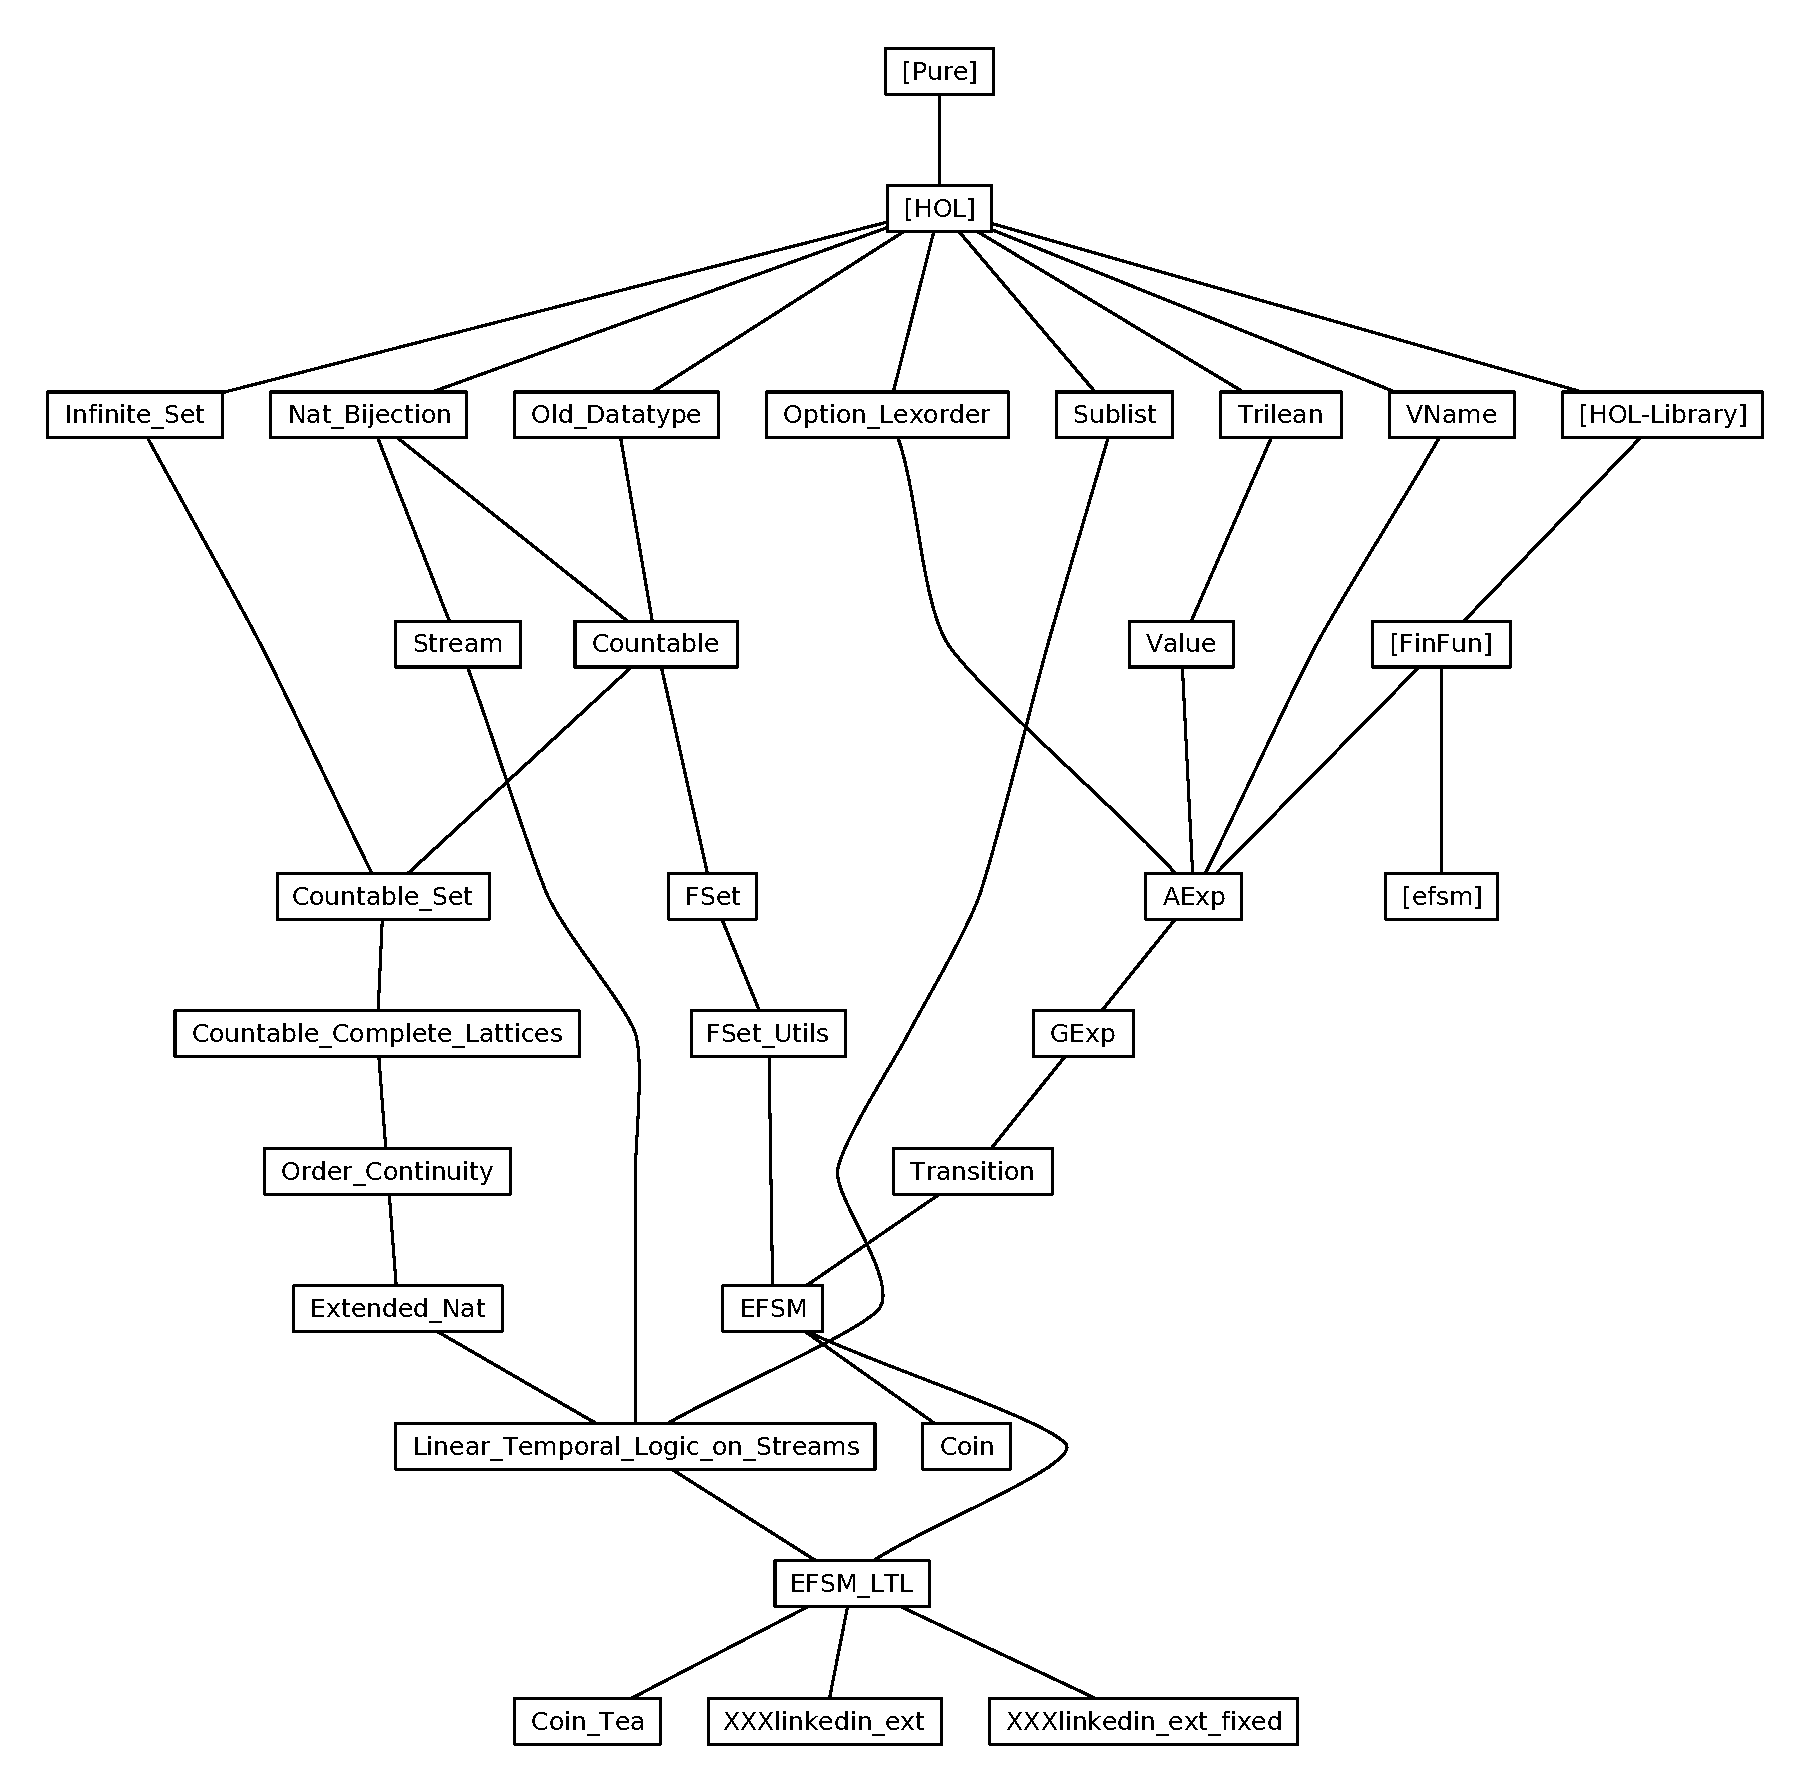
\includegraphics[height=\textheight]{session_graph}
  \caption{The Dependency Graph of the Isabelle Theories.\label{fig:session-graph}}
\end{figure}
The rest of this document is automatically generated from the
formalization in Isabelle/HOL, i.e., all content is checked by
Isabelle.  Overall, the structure of this document follows the
theory dependencies (see \autoref{fig:session-graph}):

\nocite{foster.ea:efsm:2018}

\clearpage
\chapter{Theories}

%
\begin{isabellebody}%
\setisabellecontext{liftController{\isadigit{3}}}%
%
\isadelimtheory
%
\endisadelimtheory
%
\isatagtheory
\isacommand{theory}\isamarkupfalse%
\ liftController{\isadigit{3}}\isanewline
\isakeyword{imports}\ {\isachardoublequoteopen}EFSM{\isachardot}EFSM{\isachardoublequoteclose}\isanewline
\isakeyword{begin}%
\endisatagtheory
{\isafoldtheory}%
%
\isadelimtheory
\isanewline
%
\endisadelimtheory
\isanewline
\isacommand{definition}\isamarkupfalse%
\ {\isachardoublequoteopen}continit{\isachardoublequoteclose}\ {\isacharcolon}{\isacharcolon}\ {\isachardoublequoteopen}transition{\isachardoublequoteclose}\ \isakeyword{where}\isanewline
{\isachardoublequoteopen}continit\ {\isasymequiv}\ {\isasymlparr}\isanewline
\ \ \ \ \ \ Label\ {\isacharequal}\ STR\ {\isacharprime}{\isacharprime}continit{\isacharprime}{\isacharprime}{\isacharcomma}\isanewline
\ \ \ \ \ \ Arity\ {\isacharequal}\ {\isadigit{0}}{\isacharcomma}\isanewline
\ \ \ \ \ \ Guards\ {\isacharequal}\ {\isacharbrackleft}{\isacharbrackright}{\isacharcomma}\isanewline
\ \ \ \ \ \ Outputs\ {\isacharequal}\ {\isacharbrackleft}{\isacharbrackright}{\isacharcomma}\isanewline
\ \ \ \ \ \ Updates\ {\isacharequal}\ {\isacharbrackleft}\isanewline
\ \ \ \ \ \ \ \ \ \ \ \ {\isacharparenleft}{\isadigit{1}}{\isacharcomma}\ {\isacharparenleft}L\ {\isacharparenleft}Str\ {\isacharprime}{\isacharprime}true{\isacharprime}{\isacharprime}{\isacharparenright}{\isacharparenright}{\isacharparenright}\isanewline
\ \ \ \ \ \ {\isacharbrackright}\isanewline
{\isasymrparr}{\isachardoublequoteclose}\isanewline
\isanewline
\isacommand{definition}\isamarkupfalse%
\ {\isachardoublequoteopen}motorstop{\isadigit{4}}{\isachardoublequoteclose}\ {\isacharcolon}{\isacharcolon}\ {\isachardoublequoteopen}transition{\isachardoublequoteclose}\ \isakeyword{where}\isanewline
{\isachardoublequoteopen}motorstop{\isadigit{4}}\ {\isasymequiv}\ {\isasymlparr}\isanewline
\ \ \ \ \ \ Label\ {\isacharequal}\ STR\ {\isacharprime}{\isacharprime}motorstop{\isacharprime}{\isacharprime}{\isacharcomma}\isanewline
\ \ \ \ \ \ Arity\ {\isacharequal}\ {\isadigit{2}}{\isacharcomma}\isanewline
\ \ \ \ \ \ Guards\ {\isacharequal}\ {\isacharbrackleft}\isanewline
\ \ \ \ \ \ \ \ \ \ \ \ {\isacharparenleft}Eq\ {\isacharparenleft}V\ {\isacharparenleft}R\ {\isadigit{1}}{\isacharparenright}{\isacharparenright}\ {\isacharparenleft}L\ {\isacharparenleft}Str\ {\isacharprime}{\isacharprime}true{\isacharprime}{\isacharprime}{\isacharparenright}{\isacharparenright}{\isacharparenright}{\isacharcomma}\isanewline
\ \ \ \ \ \ \ \ \ \ \ \ {\isacharparenleft}Eq\ {\isacharparenleft}V\ {\isacharparenleft}I\ {\isadigit{0}}{\isacharparenright}{\isacharparenright}\ {\isacharparenleft}L\ {\isacharparenleft}Str\ {\isacharprime}{\isacharprime}true{\isacharprime}{\isacharprime}{\isacharparenright}{\isacharparenright}{\isacharparenright}{\isacharcomma}\isanewline
\ \ \ \ \ \ \ \ \ \ \ \ {\isacharparenleft}Eq\ {\isacharparenleft}V\ {\isacharparenleft}I\ {\isadigit{1}}{\isacharparenright}{\isacharparenright}\ {\isacharparenleft}L\ {\isacharparenleft}Str\ {\isacharprime}{\isacharprime}true{\isacharprime}{\isacharprime}{\isacharparenright}{\isacharparenright}{\isacharparenright}\isanewline
\ \ \ \ \ \ {\isacharbrackright}{\isacharcomma}\isanewline
\ \ \ \ \ \ Outputs\ {\isacharequal}\ {\isacharbrackleft}\isanewline
\ \ \ \ \ \ \ \ \ \ \ \ {\isacharparenleft}L\ {\isacharparenleft}Num\ {\isadigit{0}}{\isacharparenright}{\isacharparenright}{\isacharcomma}\isanewline
\ \ \ \ \ \ \ \ \ \ \ \ {\isacharparenleft}L\ {\isacharparenleft}Num\ {\isadigit{4}}{\isacharparenright}{\isacharparenright}{\isacharcomma}\isanewline
\ \ \ \ \ \ \ \ \ \ \ \ {\isacharparenleft}L\ {\isacharparenleft}Str\ {\isacharprime}{\isacharprime}true{\isacharprime}{\isacharprime}{\isacharparenright}{\isacharparenright}\isanewline
\ \ \ \ \ \ {\isacharbrackright}{\isacharcomma}\isanewline
\ \ \ \ \ \ Updates\ {\isacharequal}\ {\isacharbrackleft}{\isacharbrackright}\isanewline
{\isasymrparr}{\isachardoublequoteclose}\isanewline
\isanewline
\isacommand{definition}\isamarkupfalse%
\ {\isachardoublequoteopen}motorstop{\isadigit{3}}{\isachardoublequoteclose}\ {\isacharcolon}{\isacharcolon}\ {\isachardoublequoteopen}transition{\isachardoublequoteclose}\ \isakeyword{where}\isanewline
{\isachardoublequoteopen}motorstop{\isadigit{3}}\ {\isasymequiv}\ {\isasymlparr}\isanewline
\ \ \ \ \ \ Label\ {\isacharequal}\ STR\ {\isacharprime}{\isacharprime}motorstop{\isacharprime}{\isacharprime}{\isacharcomma}\isanewline
\ \ \ \ \ \ Arity\ {\isacharequal}\ {\isadigit{2}}{\isacharcomma}\isanewline
\ \ \ \ \ \ Guards\ {\isacharequal}\ {\isacharbrackleft}\isanewline
\ \ \ \ \ \ \ \ \ \ \ \ {\isacharparenleft}Eq\ {\isacharparenleft}V\ {\isacharparenleft}R\ {\isadigit{1}}{\isacharparenright}{\isacharparenright}\ {\isacharparenleft}L\ {\isacharparenleft}Str\ {\isacharprime}{\isacharprime}true{\isacharprime}{\isacharprime}{\isacharparenright}{\isacharparenright}{\isacharparenright}{\isacharcomma}\isanewline
\ \ \ \ \ \ \ \ \ \ \ \ {\isacharparenleft}Eq\ {\isacharparenleft}V\ {\isacharparenleft}I\ {\isadigit{0}}{\isacharparenright}{\isacharparenright}\ {\isacharparenleft}L\ {\isacharparenleft}Str\ {\isacharprime}{\isacharprime}true{\isacharprime}{\isacharprime}{\isacharparenright}{\isacharparenright}{\isacharparenright}{\isacharcomma}\isanewline
\ \ \ \ \ \ \ \ \ \ \ \ {\isacharparenleft}Eq\ {\isacharparenleft}V\ {\isacharparenleft}I\ {\isadigit{1}}{\isacharparenright}{\isacharparenright}\ {\isacharparenleft}L\ {\isacharparenleft}Str\ {\isacharprime}{\isacharprime}true{\isacharprime}{\isacharprime}{\isacharparenright}{\isacharparenright}{\isacharparenright}\isanewline
\ \ \ \ \ \ {\isacharbrackright}{\isacharcomma}\isanewline
\ \ \ \ \ \ Outputs\ {\isacharequal}\ {\isacharbrackleft}\isanewline
\ \ \ \ \ \ \ \ \ \ \ \ {\isacharparenleft}L\ {\isacharparenleft}Num\ {\isadigit{0}}{\isacharparenright}{\isacharparenright}{\isacharcomma}\isanewline
\ \ \ \ \ \ \ \ \ \ \ \ {\isacharparenleft}L\ {\isacharparenleft}Num\ {\isadigit{3}}{\isacharparenright}{\isacharparenright}{\isacharcomma}\isanewline
\ \ \ \ \ \ \ \ \ \ \ \ {\isacharparenleft}L\ {\isacharparenleft}Str\ {\isacharprime}{\isacharprime}true{\isacharprime}{\isacharprime}{\isacharparenright}{\isacharparenright}\isanewline
\ \ \ \ \ \ {\isacharbrackright}{\isacharcomma}\isanewline
\ \ \ \ \ \ Updates\ {\isacharequal}\ {\isacharbrackleft}{\isacharbrackright}\isanewline
{\isasymrparr}{\isachardoublequoteclose}\isanewline
\isanewline
\isacommand{definition}\isamarkupfalse%
\ {\isachardoublequoteopen}motorstop{\isadigit{2}}{\isachardoublequoteclose}\ {\isacharcolon}{\isacharcolon}\ {\isachardoublequoteopen}transition{\isachardoublequoteclose}\ \isakeyword{where}\isanewline
{\isachardoublequoteopen}motorstop{\isadigit{2}}\ {\isasymequiv}\ {\isasymlparr}\isanewline
\ \ \ \ \ \ Label\ {\isacharequal}\ STR\ {\isacharprime}{\isacharprime}motorstop{\isacharprime}{\isacharprime}{\isacharcomma}\isanewline
\ \ \ \ \ \ Arity\ {\isacharequal}\ {\isadigit{2}}{\isacharcomma}\isanewline
\ \ \ \ \ \ Guards\ {\isacharequal}\ {\isacharbrackleft}\isanewline
\ \ \ \ \ \ \ \ \ \ \ \ {\isacharparenleft}Eq\ {\isacharparenleft}V\ {\isacharparenleft}R\ {\isadigit{1}}{\isacharparenright}{\isacharparenright}\ {\isacharparenleft}L\ {\isacharparenleft}Str\ {\isacharprime}{\isacharprime}true{\isacharprime}{\isacharprime}{\isacharparenright}{\isacharparenright}{\isacharparenright}{\isacharcomma}\isanewline
\ \ \ \ \ \ \ \ \ \ \ \ {\isacharparenleft}Eq\ {\isacharparenleft}V\ {\isacharparenleft}I\ {\isadigit{0}}{\isacharparenright}{\isacharparenright}\ {\isacharparenleft}L\ {\isacharparenleft}Str\ {\isacharprime}{\isacharprime}true{\isacharprime}{\isacharprime}{\isacharparenright}{\isacharparenright}{\isacharparenright}{\isacharcomma}\isanewline
\ \ \ \ \ \ \ \ \ \ \ \ {\isacharparenleft}Eq\ {\isacharparenleft}V\ {\isacharparenleft}I\ {\isadigit{1}}{\isacharparenright}{\isacharparenright}\ {\isacharparenleft}L\ {\isacharparenleft}Str\ {\isacharprime}{\isacharprime}true{\isacharprime}{\isacharprime}{\isacharparenright}{\isacharparenright}{\isacharparenright}\isanewline
\ \ \ \ \ \ {\isacharbrackright}{\isacharcomma}\isanewline
\ \ \ \ \ \ Outputs\ {\isacharequal}\ {\isacharbrackleft}\isanewline
\ \ \ \ \ \ \ \ \ \ \ \ {\isacharparenleft}L\ {\isacharparenleft}Num\ {\isadigit{0}}{\isacharparenright}{\isacharparenright}{\isacharcomma}\isanewline
\ \ \ \ \ \ \ \ \ \ \ \ {\isacharparenleft}L\ {\isacharparenleft}Num\ {\isadigit{2}}{\isacharparenright}{\isacharparenright}{\isacharcomma}\isanewline
\ \ \ \ \ \ \ \ \ \ \ \ {\isacharparenleft}L\ {\isacharparenleft}Str\ {\isacharprime}{\isacharprime}true{\isacharprime}{\isacharprime}{\isacharparenright}{\isacharparenright}\isanewline
\ \ \ \ \ \ {\isacharbrackright}{\isacharcomma}\isanewline
\ \ \ \ \ \ Updates\ {\isacharequal}\ {\isacharbrackleft}{\isacharbrackright}\isanewline
{\isasymrparr}{\isachardoublequoteclose}\isanewline
\isanewline
\isacommand{definition}\isamarkupfalse%
\ {\isachardoublequoteopen}motorstop{\isadigit{1}}{\isachardoublequoteclose}\ {\isacharcolon}{\isacharcolon}\ {\isachardoublequoteopen}transition{\isachardoublequoteclose}\ \isakeyword{where}\isanewline
{\isachardoublequoteopen}motorstop{\isadigit{1}}\ {\isasymequiv}\ {\isasymlparr}\isanewline
\ \ \ \ \ \ Label\ {\isacharequal}\ STR\ {\isacharprime}{\isacharprime}motorstop{\isacharprime}{\isacharprime}{\isacharcomma}\isanewline
\ \ \ \ \ \ Arity\ {\isacharequal}\ {\isadigit{2}}{\isacharcomma}\isanewline
\ \ \ \ \ \ Guards\ {\isacharequal}\ {\isacharbrackleft}\isanewline
\ \ \ \ \ \ \ \ \ \ \ \ {\isacharparenleft}Eq\ {\isacharparenleft}V\ {\isacharparenleft}R\ {\isadigit{1}}{\isacharparenright}{\isacharparenright}\ {\isacharparenleft}L\ {\isacharparenleft}Str\ {\isacharprime}{\isacharprime}true{\isacharprime}{\isacharprime}{\isacharparenright}{\isacharparenright}{\isacharparenright}{\isacharcomma}\isanewline
\ \ \ \ \ \ \ \ \ \ \ \ {\isacharparenleft}Eq\ {\isacharparenleft}V\ {\isacharparenleft}I\ {\isadigit{0}}{\isacharparenright}{\isacharparenright}\ {\isacharparenleft}L\ {\isacharparenleft}Str\ {\isacharprime}{\isacharprime}true{\isacharprime}{\isacharprime}{\isacharparenright}{\isacharparenright}{\isacharparenright}{\isacharcomma}\isanewline
\ \ \ \ \ \ \ \ \ \ \ \ {\isacharparenleft}Eq\ {\isacharparenleft}V\ {\isacharparenleft}I\ {\isadigit{1}}{\isacharparenright}{\isacharparenright}\ {\isacharparenleft}L\ {\isacharparenleft}Str\ {\isacharprime}{\isacharprime}true{\isacharprime}{\isacharprime}{\isacharparenright}{\isacharparenright}{\isacharparenright}\isanewline
\ \ \ \ \ \ {\isacharbrackright}{\isacharcomma}\isanewline
\ \ \ \ \ \ Outputs\ {\isacharequal}\ {\isacharbrackleft}\isanewline
\ \ \ \ \ \ \ \ \ \ \ \ {\isacharparenleft}L\ {\isacharparenleft}Num\ {\isadigit{0}}{\isacharparenright}{\isacharparenright}{\isacharcomma}\isanewline
\ \ \ \ \ \ \ \ \ \ \ \ {\isacharparenleft}L\ {\isacharparenleft}Num\ {\isadigit{1}}{\isacharparenright}{\isacharparenright}{\isacharcomma}\isanewline
\ \ \ \ \ \ \ \ \ \ \ \ {\isacharparenleft}L\ {\isacharparenleft}Str\ {\isacharprime}{\isacharprime}true{\isacharprime}{\isacharprime}{\isacharparenright}{\isacharparenright}\isanewline
\ \ \ \ \ \ {\isacharbrackright}{\isacharcomma}\isanewline
\ \ \ \ \ \ Updates\ {\isacharequal}\ {\isacharbrackleft}{\isacharbrackright}\isanewline
{\isasymrparr}{\isachardoublequoteclose}\isanewline
\isanewline
\isacommand{abbreviation}\isamarkupfalse%
\ {\isachardoublequoteopen}startsearch{\isachardoublequoteclose}\ {\isacharcolon}{\isacharcolon}\ {\isachardoublequoteopen}transition{\isachardoublequoteclose}\ \isakeyword{where}\isanewline
{\isachardoublequoteopen}startsearch\ {\isasymequiv}\ {\isasymlparr}\isanewline
\ \ \ \ \ \ Label\ {\isacharequal}\ STR\ {\isacharprime}{\isacharprime}startsearch{\isacharprime}{\isacharprime}{\isacharcomma}\isanewline
\ \ \ \ \ \ Arity\ {\isacharequal}\ {\isadigit{2}}{\isacharcomma}\isanewline
\ \ \ \ \ \ Guards\ {\isacharequal}\ {\isacharbrackleft}\isanewline
\ \ \ \ \ \ \ \ \ \ \ \ {\isacharparenleft}Eq\ {\isacharparenleft}V\ {\isacharparenleft}I\ {\isadigit{0}}{\isacharparenright}{\isacharparenright}\ {\isacharparenleft}L\ {\isacharparenleft}Str\ {\isacharprime}{\isacharprime}true{\isacharprime}{\isacharprime}{\isacharparenright}{\isacharparenright}{\isacharparenright}{\isacharcomma}\isanewline
\ \ \ \ \ \ \ \ \ \ \ \ {\isacharparenleft}Eq\ {\isacharparenleft}V\ {\isacharparenleft}I\ {\isadigit{1}}{\isacharparenright}{\isacharparenright}\ {\isacharparenleft}L\ {\isacharparenleft}Str\ {\isacharprime}{\isacharprime}false{\isacharprime}{\isacharprime}{\isacharparenright}{\isacharparenright}{\isacharparenright}\isanewline
\ \ \ \ \ \ {\isacharbrackright}{\isacharcomma}\isanewline
\ \ \ \ \ \ Outputs\ {\isacharequal}\ {\isacharbrackleft}{\isacharbrackright}{\isacharcomma}\isanewline
\ \ \ \ \ \ Updates\ {\isacharequal}\ {\isacharbrackleft}{\isacharbrackright}\isanewline
{\isasymrparr}{\isachardoublequoteclose}\isanewline
\isanewline
\isacommand{definition}\isamarkupfalse%
\ {\isachardoublequoteopen}opendoor{\isadigit{4}}{\isachardoublequoteclose}\ {\isacharcolon}{\isacharcolon}\ {\isachardoublequoteopen}transition{\isachardoublequoteclose}\ \isakeyword{where}\isanewline
{\isachardoublequoteopen}opendoor{\isadigit{4}}\ {\isasymequiv}\ {\isasymlparr}\isanewline
\ \ \ \ \ \ Label\ {\isacharequal}\ STR\ {\isacharprime}{\isacharprime}opendoor{\isacharprime}{\isacharprime}{\isacharcomma}\isanewline
\ \ \ \ \ \ Arity\ {\isacharequal}\ {\isadigit{1}}{\isacharcomma}\isanewline
\ \ \ \ \ \ Guards\ {\isacharequal}\ {\isacharbrackleft}\isanewline
\ \ \ \ \ \ \ \ \ \ \ \ {\isacharparenleft}Eq\ {\isacharparenleft}V\ {\isacharparenleft}I\ {\isadigit{0}}{\isacharparenright}{\isacharparenright}\ {\isacharparenleft}L\ {\isacharparenleft}Str\ {\isacharprime}{\isacharprime}true{\isacharprime}{\isacharprime}{\isacharparenright}{\isacharparenright}{\isacharparenright}\isanewline
\ \ \ \ \ \ {\isacharbrackright}{\isacharcomma}\isanewline
\ \ \ \ \ \ Outputs\ {\isacharequal}\ {\isacharbrackleft}\isanewline
\ \ \ \ \ \ \ \ \ \ \ \ {\isacharparenleft}L\ {\isacharparenleft}Str\ {\isacharprime}{\isacharprime}true{\isacharprime}{\isacharprime}{\isacharparenright}{\isacharparenright}{\isacharcomma}\isanewline
\ \ \ \ \ \ \ \ \ \ \ \ {\isacharparenleft}L\ {\isacharparenleft}Num\ {\isadigit{4}}{\isacharparenright}{\isacharparenright}\isanewline
\ \ \ \ \ \ {\isacharbrackright}{\isacharcomma}\isanewline
\ \ \ \ \ \ Updates\ {\isacharequal}\ {\isacharbrackleft}{\isacharbrackright}\isanewline
{\isasymrparr}{\isachardoublequoteclose}\isanewline
\isanewline
\isacommand{definition}\isamarkupfalse%
\ {\isachardoublequoteopen}opendoor{\isadigit{3}}{\isachardoublequoteclose}\ {\isacharcolon}{\isacharcolon}\ {\isachardoublequoteopen}transition{\isachardoublequoteclose}\ \isakeyword{where}\isanewline
{\isachardoublequoteopen}opendoor{\isadigit{3}}\ {\isasymequiv}\ {\isasymlparr}\isanewline
\ \ \ \ \ \ Label\ {\isacharequal}\ STR\ {\isacharprime}{\isacharprime}opendoor{\isacharprime}{\isacharprime}{\isacharcomma}\isanewline
\ \ \ \ \ \ Arity\ {\isacharequal}\ {\isadigit{1}}{\isacharcomma}\isanewline
\ \ \ \ \ \ Guards\ {\isacharequal}\ {\isacharbrackleft}\isanewline
\ \ \ \ \ \ \ \ \ \ \ \ {\isacharparenleft}Eq\ {\isacharparenleft}V\ {\isacharparenleft}I\ {\isadigit{0}}{\isacharparenright}{\isacharparenright}\ {\isacharparenleft}L\ {\isacharparenleft}Str\ {\isacharprime}{\isacharprime}true{\isacharprime}{\isacharprime}{\isacharparenright}{\isacharparenright}{\isacharparenright}\isanewline
\ \ \ \ \ \ {\isacharbrackright}{\isacharcomma}\isanewline
\ \ \ \ \ \ Outputs\ {\isacharequal}\ {\isacharbrackleft}\isanewline
\ \ \ \ \ \ \ \ \ \ \ \ {\isacharparenleft}L\ {\isacharparenleft}Str\ {\isacharprime}{\isacharprime}true{\isacharprime}{\isacharprime}{\isacharparenright}{\isacharparenright}{\isacharcomma}\isanewline
\ \ \ \ \ \ \ \ \ \ \ \ {\isacharparenleft}L\ {\isacharparenleft}Num\ {\isadigit{3}}{\isacharparenright}{\isacharparenright}\isanewline
\ \ \ \ \ \ {\isacharbrackright}{\isacharcomma}\isanewline
\ \ \ \ \ \ Updates\ {\isacharequal}\ {\isacharbrackleft}{\isacharbrackright}\isanewline
{\isasymrparr}{\isachardoublequoteclose}\isanewline
\isanewline
\isacommand{definition}\isamarkupfalse%
\ {\isachardoublequoteopen}opendoor{\isadigit{2}}{\isachardoublequoteclose}\ {\isacharcolon}{\isacharcolon}\ {\isachardoublequoteopen}transition{\isachardoublequoteclose}\ \isakeyword{where}\isanewline
{\isachardoublequoteopen}opendoor{\isadigit{2}}\ {\isasymequiv}\ {\isasymlparr}\isanewline
\ \ \ \ \ \ Label\ {\isacharequal}\ STR\ {\isacharprime}{\isacharprime}opendoor{\isacharprime}{\isacharprime}{\isacharcomma}\isanewline
\ \ \ \ \ \ Arity\ {\isacharequal}\ {\isadigit{1}}{\isacharcomma}\isanewline
\ \ \ \ \ \ Guards\ {\isacharequal}\ {\isacharbrackleft}\isanewline
\ \ \ \ \ \ \ \ \ \ \ \ {\isacharparenleft}Eq\ {\isacharparenleft}V\ {\isacharparenleft}I\ {\isadigit{0}}{\isacharparenright}{\isacharparenright}\ {\isacharparenleft}L\ {\isacharparenleft}Str\ {\isacharprime}{\isacharprime}true{\isacharprime}{\isacharprime}{\isacharparenright}{\isacharparenright}{\isacharparenright}\isanewline
\ \ \ \ \ \ {\isacharbrackright}{\isacharcomma}\isanewline
\ \ \ \ \ \ Outputs\ {\isacharequal}\ {\isacharbrackleft}\isanewline
\ \ \ \ \ \ \ \ \ \ \ \ {\isacharparenleft}L\ {\isacharparenleft}Str\ {\isacharprime}{\isacharprime}true{\isacharprime}{\isacharprime}{\isacharparenright}{\isacharparenright}{\isacharcomma}\isanewline
\ \ \ \ \ \ \ \ \ \ \ \ {\isacharparenleft}L\ {\isacharparenleft}Num\ {\isadigit{2}}{\isacharparenright}{\isacharparenright}\isanewline
\ \ \ \ \ \ {\isacharbrackright}{\isacharcomma}\isanewline
\ \ \ \ \ \ Updates\ {\isacharequal}\ {\isacharbrackleft}{\isacharbrackright}\isanewline
{\isasymrparr}{\isachardoublequoteclose}\isanewline
\isanewline
\isacommand{definition}\isamarkupfalse%
\ {\isachardoublequoteopen}opendoor{\isadigit{1}}{\isachardoublequoteclose}\ {\isacharcolon}{\isacharcolon}\ {\isachardoublequoteopen}transition{\isachardoublequoteclose}\ \isakeyword{where}\isanewline
{\isachardoublequoteopen}opendoor{\isadigit{1}}\ {\isasymequiv}\ {\isasymlparr}\isanewline
\ \ \ \ \ \ Label\ {\isacharequal}\ STR\ {\isacharprime}{\isacharprime}opendoor{\isacharprime}{\isacharprime}{\isacharcomma}\isanewline
\ \ \ \ \ \ Arity\ {\isacharequal}\ {\isadigit{1}}{\isacharcomma}\isanewline
\ \ \ \ \ \ Guards\ {\isacharequal}\ {\isacharbrackleft}\isanewline
\ \ \ \ \ \ \ \ \ \ \ \ {\isacharparenleft}Eq\ {\isacharparenleft}V\ {\isacharparenleft}I\ {\isadigit{0}}{\isacharparenright}{\isacharparenright}\ {\isacharparenleft}L\ {\isacharparenleft}Str\ {\isacharprime}{\isacharprime}true{\isacharprime}{\isacharprime}{\isacharparenright}{\isacharparenright}{\isacharparenright}\isanewline
\ \ \ \ \ \ {\isacharbrackright}{\isacharcomma}\isanewline
\ \ \ \ \ \ Outputs\ {\isacharequal}\ {\isacharbrackleft}\isanewline
\ \ \ \ \ \ \ \ \ \ \ \ {\isacharparenleft}L\ {\isacharparenleft}Str\ {\isacharprime}{\isacharprime}true{\isacharprime}{\isacharprime}{\isacharparenright}{\isacharparenright}{\isacharcomma}\isanewline
\ \ \ \ \ \ \ \ \ \ \ \ {\isacharparenleft}L\ {\isacharparenleft}Num\ {\isadigit{1}}{\isacharparenright}{\isacharparenright}\isanewline
\ \ \ \ \ \ {\isacharbrackright}{\isacharcomma}\isanewline
\ \ \ \ \ \ Updates\ {\isacharequal}\ {\isacharbrackleft}{\isacharbrackright}\isanewline
{\isasymrparr}{\isachardoublequoteclose}\isanewline
\isanewline
\isacommand{definition}\isamarkupfalse%
\ {\isachardoublequoteopen}return{\isadigit{4}}{\isachardoublequoteclose}\ {\isacharcolon}{\isacharcolon}\ {\isachardoublequoteopen}transition{\isachardoublequoteclose}\ \isakeyword{where}\isanewline
{\isachardoublequoteopen}return{\isadigit{4}}\ {\isasymequiv}\ {\isasymlparr}\isanewline
\ \ \ \ \ \ Label\ {\isacharequal}\ STR\ {\isacharprime}{\isacharprime}return{\isacharprime}{\isacharprime}{\isacharcomma}\isanewline
\ \ \ \ \ \ Arity\ {\isacharequal}\ {\isadigit{0}}{\isacharcomma}\isanewline
\ \ \ \ \ \ Guards\ {\isacharequal}\ {\isacharbrackleft}\isanewline
\ \ \ \ \ \ \ \ \ \ \ \ {\isacharparenleft}Eq\ {\isacharparenleft}V\ {\isacharparenleft}R\ {\isadigit{4}}{\isacharparenright}{\isacharparenright}\ {\isacharparenleft}L\ {\isacharparenleft}Num\ {\isadigit{4}}{\isacharparenright}{\isacharparenright}{\isacharparenright}\isanewline
\ \ \ \ \ \ {\isacharbrackright}{\isacharcomma}\isanewline
\ \ \ \ \ \ Outputs\ {\isacharequal}\ {\isacharbrackleft}{\isacharbrackright}{\isacharcomma}\isanewline
\ \ \ \ \ \ Updates\ {\isacharequal}\ {\isacharbrackleft}{\isacharbrackright}\isanewline
{\isasymrparr}{\isachardoublequoteclose}\isanewline
\isanewline
\isacommand{definition}\isamarkupfalse%
\ {\isachardoublequoteopen}return{\isadigit{3}}{\isachardoublequoteclose}\ {\isacharcolon}{\isacharcolon}\ {\isachardoublequoteopen}transition{\isachardoublequoteclose}\ \isakeyword{where}\isanewline
{\isachardoublequoteopen}return{\isadigit{3}}\ {\isasymequiv}\ {\isasymlparr}\isanewline
\ \ \ \ \ \ Label\ {\isacharequal}\ STR\ {\isacharprime}{\isacharprime}return{\isacharprime}{\isacharprime}{\isacharcomma}\isanewline
\ \ \ \ \ \ Arity\ {\isacharequal}\ {\isadigit{0}}{\isacharcomma}\isanewline
\ \ \ \ \ \ Guards\ {\isacharequal}\ {\isacharbrackleft}\isanewline
\ \ \ \ \ \ \ \ \ \ \ \ {\isacharparenleft}Eq\ {\isacharparenleft}V\ {\isacharparenleft}R\ {\isadigit{4}}{\isacharparenright}{\isacharparenright}\ {\isacharparenleft}L\ {\isacharparenleft}Num\ {\isadigit{3}}{\isacharparenright}{\isacharparenright}{\isacharparenright}\isanewline
\ \ \ \ \ \ {\isacharbrackright}{\isacharcomma}\isanewline
\ \ \ \ \ \ Outputs\ {\isacharequal}\ {\isacharbrackleft}{\isacharbrackright}{\isacharcomma}\isanewline
\ \ \ \ \ \ Updates\ {\isacharequal}\ {\isacharbrackleft}{\isacharbrackright}\isanewline
{\isasymrparr}{\isachardoublequoteclose}\isanewline
\isanewline
\isacommand{definition}\isamarkupfalse%
\ {\isachardoublequoteopen}return{\isadigit{2}}{\isachardoublequoteclose}\ {\isacharcolon}{\isacharcolon}\ {\isachardoublequoteopen}transition{\isachardoublequoteclose}\ \isakeyword{where}\isanewline
{\isachardoublequoteopen}return{\isadigit{2}}\ {\isasymequiv}\ {\isasymlparr}\isanewline
\ \ \ \ \ \ Label\ {\isacharequal}\ STR\ {\isacharprime}{\isacharprime}return{\isacharprime}{\isacharprime}{\isacharcomma}\isanewline
\ \ \ \ \ \ Arity\ {\isacharequal}\ {\isadigit{0}}{\isacharcomma}\isanewline
\ \ \ \ \ \ Guards\ {\isacharequal}\ {\isacharbrackleft}\isanewline
\ \ \ \ \ \ \ \ \ \ \ \ {\isacharparenleft}Eq\ {\isacharparenleft}V\ {\isacharparenleft}R\ {\isadigit{4}}{\isacharparenright}{\isacharparenright}\ {\isacharparenleft}L\ {\isacharparenleft}Num\ {\isadigit{2}}{\isacharparenright}{\isacharparenright}{\isacharparenright}\isanewline
\ \ \ \ \ \ {\isacharbrackright}{\isacharcomma}\isanewline
\ \ \ \ \ \ Outputs\ {\isacharequal}\ {\isacharbrackleft}{\isacharbrackright}{\isacharcomma}\isanewline
\ \ \ \ \ \ Updates\ {\isacharequal}\ {\isacharbrackleft}{\isacharbrackright}\isanewline
{\isasymrparr}{\isachardoublequoteclose}\isanewline
\isanewline
\isacommand{definition}\isamarkupfalse%
\ {\isachardoublequoteopen}return{\isadigit{1}}{\isachardoublequoteclose}\ {\isacharcolon}{\isacharcolon}\ {\isachardoublequoteopen}transition{\isachardoublequoteclose}\ \isakeyword{where}\isanewline
{\isachardoublequoteopen}return{\isadigit{1}}\ {\isasymequiv}\ {\isasymlparr}\isanewline
\ \ \ \ \ \ Label\ {\isacharequal}\ STR\ {\isacharprime}{\isacharprime}return{\isacharprime}{\isacharprime}{\isacharcomma}\isanewline
\ \ \ \ \ \ Arity\ {\isacharequal}\ {\isadigit{0}}{\isacharcomma}\isanewline
\ \ \ \ \ \ Guards\ {\isacharequal}\ {\isacharbrackleft}\isanewline
\ \ \ \ \ \ \ \ \ \ \ \ {\isacharparenleft}Eq\ {\isacharparenleft}V\ {\isacharparenleft}R\ {\isadigit{4}}{\isacharparenright}{\isacharparenright}\ {\isacharparenleft}L\ {\isacharparenleft}Num\ {\isadigit{1}}{\isacharparenright}{\isacharparenright}{\isacharparenright}\isanewline
\ \ \ \ \ \ {\isacharbrackright}{\isacharcomma}\isanewline
\ \ \ \ \ \ Outputs\ {\isacharequal}\ {\isacharbrackleft}{\isacharbrackright}{\isacharcomma}\isanewline
\ \ \ \ \ \ Updates\ {\isacharequal}\ {\isacharbrackleft}{\isacharbrackright}\isanewline
{\isasymrparr}{\isachardoublequoteclose}\isanewline
\isanewline
\isacommand{definition}\isamarkupfalse%
\ {\isachardoublequoteopen}down{\isadigit{4}}{\isadigit{3}}stop{\isachardoublequoteclose}\ {\isacharcolon}{\isacharcolon}\ {\isachardoublequoteopen}transition{\isachardoublequoteclose}\ \isakeyword{where}\isanewline
{\isachardoublequoteopen}down{\isadigit{4}}{\isadigit{3}}stop\ {\isasymequiv}\ {\isasymlparr}\isanewline
\ \ \ \ \ \ Label\ {\isacharequal}\ STR\ {\isacharprime}{\isacharprime}down{\isacharprime}{\isacharprime}{\isacharcomma}\isanewline
\ \ \ \ \ \ Arity\ {\isacharequal}\ {\isadigit{3}}{\isacharcomma}\isanewline
\ \ \ \ \ \ Guards\ {\isacharequal}\ {\isacharbrackleft}\isanewline
\ \ \ \ \ \ \ \ \ \ \ \ {\isacharparenleft}Eq\ {\isacharparenleft}V\ {\isacharparenleft}R\ {\isadigit{2}}{\isacharparenright}{\isacharparenright}\ {\isacharparenleft}L\ {\isacharparenleft}Num\ {\isadigit{2}}{\isacharparenright}{\isacharparenright}{\isacharparenright}{\isacharcomma}\isanewline
\ \ \ \ \ \ \ \ \ \ \ \ {\isacharparenleft}Eq\ {\isacharparenleft}V\ {\isacharparenleft}R\ {\isadigit{1}}{\isacharparenright}{\isacharparenright}\ {\isacharparenleft}L\ {\isacharparenleft}Str\ {\isacharprime}{\isacharprime}false{\isacharprime}{\isacharprime}{\isacharparenright}{\isacharparenright}{\isacharparenright}{\isacharcomma}\isanewline
\ \ \ \ \ \ \ \ \ \ \ \ {\isacharparenleft}Eq\ {\isacharparenleft}V\ {\isacharparenleft}I\ {\isadigit{0}}{\isacharparenright}{\isacharparenright}\ {\isacharparenleft}L\ {\isacharparenleft}Str\ {\isacharprime}{\isacharprime}true{\isacharprime}{\isacharprime}{\isacharparenright}{\isacharparenright}{\isacharparenright}{\isacharcomma}\isanewline
\ \ \ \ \ \ \ \ \ \ \ \ {\isacharparenleft}Eq\ {\isacharparenleft}V\ {\isacharparenleft}I\ {\isadigit{1}}{\isacharparenright}{\isacharparenright}\ {\isacharparenleft}L\ {\isacharparenleft}Str\ {\isacharprime}{\isacharprime}true{\isacharprime}{\isacharprime}{\isacharparenright}{\isacharparenright}{\isacharparenright}{\isacharcomma}\isanewline
\ \ \ \ \ \ \ \ \ \ \ \ {\isacharparenleft}Eq\ {\isacharparenleft}V\ {\isacharparenleft}I\ {\isadigit{2}}{\isacharparenright}{\isacharparenright}\ {\isacharparenleft}L\ {\isacharparenleft}Str\ {\isacharprime}{\isacharprime}true{\isacharprime}{\isacharprime}{\isacharparenright}{\isacharparenright}{\isacharparenright}\isanewline
\ \ \ \ \ \ {\isacharbrackright}{\isacharcomma}\isanewline
\ \ \ \ \ \ Outputs\ {\isacharequal}\ {\isacharbrackleft}\isanewline
\ \ \ \ \ \ \ \ \ \ \ \ {\isacharparenleft}L\ {\isacharparenleft}Num\ {\isadigit{2}}{\isacharparenright}{\isacharparenright}{\isacharcomma}\isanewline
\ \ \ \ \ \ \ \ \ \ \ \ {\isacharparenleft}L\ {\isacharparenleft}Str\ {\isacharprime}{\isacharprime}true{\isacharprime}{\isacharprime}{\isacharparenright}{\isacharparenright}\isanewline
\ \ \ \ \ \ {\isacharbrackright}{\isacharcomma}\isanewline
\ \ \ \ \ \ Updates\ {\isacharequal}\ {\isacharbrackleft}\isanewline
\ \ \ \ \ \ \ \ \ \ \ \ {\isacharparenleft}{\isadigit{4}}{\isacharcomma}\ {\isacharparenleft}L\ {\isacharparenleft}Num\ {\isadigit{3}}{\isacharparenright}{\isacharparenright}{\isacharparenright}{\isacharcomma}\isanewline
\ \ \ \ \ \ \ \ \ \ \ \ {\isacharparenleft}{\isadigit{1}}{\isacharcomma}\ {\isacharparenleft}L\ {\isacharparenleft}Str\ {\isacharprime}{\isacharprime}true{\isacharprime}{\isacharprime}{\isacharparenright}{\isacharparenright}{\isacharparenright}\isanewline
\ \ \ \ \ \ {\isacharbrackright}\isanewline
{\isasymrparr}{\isachardoublequoteclose}\isanewline
\isanewline
\isacommand{definition}\isamarkupfalse%
\ {\isachardoublequoteopen}down{\isadigit{4}}{\isadigit{3}}{\isachardoublequoteclose}\ {\isacharcolon}{\isacharcolon}\ {\isachardoublequoteopen}transition{\isachardoublequoteclose}\ \isakeyword{where}\isanewline
{\isachardoublequoteopen}down{\isadigit{4}}{\isadigit{3}}\ {\isasymequiv}\ {\isasymlparr}\isanewline
\ \ \ \ \ \ Label\ {\isacharequal}\ STR\ {\isacharprime}{\isacharprime}down{\isacharprime}{\isacharprime}{\isacharcomma}\isanewline
\ \ \ \ \ \ Arity\ {\isacharequal}\ {\isadigit{3}}{\isacharcomma}\isanewline
\ \ \ \ \ \ Guards\ {\isacharequal}\ {\isacharbrackleft}\isanewline
\ \ \ \ \ \ \ \ \ \ \ \ {\isacharparenleft}Eq\ {\isacharparenleft}V\ {\isacharparenleft}R\ {\isadigit{2}}{\isacharparenright}{\isacharparenright}\ {\isacharparenleft}L\ {\isacharparenleft}Num\ {\isadigit{2}}{\isacharparenright}{\isacharparenright}{\isacharparenright}{\isacharcomma}\isanewline
\ \ \ \ \ \ \ \ \ \ \ \ {\isacharparenleft}Eq\ {\isacharparenleft}V\ {\isacharparenleft}R\ {\isadigit{1}}{\isacharparenright}{\isacharparenright}\ {\isacharparenleft}L\ {\isacharparenleft}Str\ {\isacharprime}{\isacharprime}false{\isacharprime}{\isacharprime}{\isacharparenright}{\isacharparenright}{\isacharparenright}{\isacharcomma}\isanewline
\ \ \ \ \ \ \ \ \ \ \ \ {\isacharparenleft}Eq\ {\isacharparenleft}V\ {\isacharparenleft}I\ {\isadigit{0}}{\isacharparenright}{\isacharparenright}\ {\isacharparenleft}L\ {\isacharparenleft}Str\ {\isacharprime}{\isacharprime}true{\isacharprime}{\isacharprime}{\isacharparenright}{\isacharparenright}{\isacharparenright}{\isacharcomma}\isanewline
\ \ \ \ \ \ \ \ \ \ \ \ {\isacharparenleft}Eq\ {\isacharparenleft}V\ {\isacharparenleft}I\ {\isadigit{1}}{\isacharparenright}{\isacharparenright}\ {\isacharparenleft}L\ {\isacharparenleft}Str\ {\isacharprime}{\isacharprime}true{\isacharprime}{\isacharprime}{\isacharparenright}{\isacharparenright}{\isacharparenright}{\isacharcomma}\isanewline
\ \ \ \ \ \ \ \ \ \ \ \ {\isacharparenleft}Eq\ {\isacharparenleft}V\ {\isacharparenleft}I\ {\isadigit{2}}{\isacharparenright}{\isacharparenright}\ {\isacharparenleft}L\ {\isacharparenleft}Str\ {\isacharprime}{\isacharprime}false{\isacharprime}{\isacharprime}{\isacharparenright}{\isacharparenright}{\isacharparenright}\isanewline
\ \ \ \ \ \ {\isacharbrackright}{\isacharcomma}\isanewline
\ \ \ \ \ \ Outputs\ {\isacharequal}\ {\isacharbrackleft}\isanewline
\ \ \ \ \ \ \ \ \ \ \ \ {\isacharparenleft}L\ {\isacharparenleft}Num\ {\isadigit{2}}{\isacharparenright}{\isacharparenright}{\isacharcomma}\isanewline
\ \ \ \ \ \ \ \ \ \ \ \ {\isacharparenleft}L\ {\isacharparenleft}Str\ {\isacharprime}{\isacharprime}false{\isacharprime}{\isacharprime}{\isacharparenright}{\isacharparenright}\isanewline
\ \ \ \ \ \ {\isacharbrackright}{\isacharcomma}\isanewline
\ \ \ \ \ \ Updates\ {\isacharequal}\ {\isacharbrackleft}\isanewline
\ \ \ \ \ \ \ \ \ \ \ \ {\isacharparenleft}{\isadigit{4}}{\isacharcomma}\ {\isacharparenleft}L\ {\isacharparenleft}Num\ {\isadigit{3}}{\isacharparenright}{\isacharparenright}{\isacharparenright}{\isacharcomma}\isanewline
\ \ \ \ \ \ \ \ \ \ \ \ {\isacharparenleft}{\isadigit{1}}{\isacharcomma}\ {\isacharparenleft}L\ {\isacharparenleft}Str\ {\isacharprime}{\isacharprime}false{\isacharprime}{\isacharprime}{\isacharparenright}{\isacharparenright}{\isacharparenright}\isanewline
\ \ \ \ \ \ {\isacharbrackright}\isanewline
{\isasymrparr}{\isachardoublequoteclose}\isanewline
\isanewline
\isacommand{definition}\isamarkupfalse%
\ {\isachardoublequoteopen}up{\isadigit{3}}{\isadigit{4}}stop{\isachardoublequoteclose}\ {\isacharcolon}{\isacharcolon}\ {\isachardoublequoteopen}transition{\isachardoublequoteclose}\ \isakeyword{where}\isanewline
{\isachardoublequoteopen}up{\isadigit{3}}{\isadigit{4}}stop\ {\isasymequiv}\ {\isasymlparr}\isanewline
\ \ \ \ \ \ Label\ {\isacharequal}\ STR\ {\isacharprime}{\isacharprime}up{\isacharprime}{\isacharprime}{\isacharcomma}\isanewline
\ \ \ \ \ \ Arity\ {\isacharequal}\ {\isadigit{2}}{\isacharcomma}\isanewline
\ \ \ \ \ \ Guards\ {\isacharequal}\ {\isacharbrackleft}\isanewline
\ \ \ \ \ \ \ \ \ \ \ \ {\isacharparenleft}Eq\ {\isacharparenleft}V\ {\isacharparenleft}R\ {\isadigit{2}}{\isacharparenright}{\isacharparenright}\ {\isacharparenleft}L\ {\isacharparenleft}Num\ {\isadigit{1}}{\isacharparenright}{\isacharparenright}{\isacharparenright}{\isacharcomma}\isanewline
\ \ \ \ \ \ \ \ \ \ \ \ {\isacharparenleft}Eq\ {\isacharparenleft}V\ {\isacharparenleft}R\ {\isadigit{1}}{\isacharparenright}{\isacharparenright}\ {\isacharparenleft}L\ {\isacharparenleft}Str\ {\isacharprime}{\isacharprime}false{\isacharprime}{\isacharprime}{\isacharparenright}{\isacharparenright}{\isacharparenright}{\isacharcomma}\isanewline
\ \ \ \ \ \ \ \ \ \ \ \ {\isacharparenleft}Eq\ {\isacharparenleft}V\ {\isacharparenleft}I\ {\isadigit{0}}{\isacharparenright}{\isacharparenright}\ {\isacharparenleft}L\ {\isacharparenleft}Str\ {\isacharprime}{\isacharprime}true{\isacharprime}{\isacharprime}{\isacharparenright}{\isacharparenright}{\isacharparenright}{\isacharcomma}\isanewline
\ \ \ \ \ \ \ \ \ \ \ \ {\isacharparenleft}Eq\ {\isacharparenleft}V\ {\isacharparenleft}I\ {\isadigit{1}}{\isacharparenright}{\isacharparenright}\ {\isacharparenleft}L\ {\isacharparenleft}Str\ {\isacharprime}{\isacharprime}true{\isacharprime}{\isacharprime}{\isacharparenright}{\isacharparenright}{\isacharparenright}\isanewline
\ \ \ \ \ \ {\isacharbrackright}{\isacharcomma}\isanewline
\ \ \ \ \ \ Outputs\ {\isacharequal}\ {\isacharbrackleft}\isanewline
\ \ \ \ \ \ \ \ \ \ \ \ {\isacharparenleft}L\ {\isacharparenleft}Num\ {\isadigit{1}}{\isacharparenright}{\isacharparenright}{\isacharcomma}\isanewline
\ \ \ \ \ \ \ \ \ \ \ \ {\isacharparenleft}L\ {\isacharparenleft}Str\ {\isacharprime}{\isacharprime}true{\isacharprime}{\isacharprime}{\isacharparenright}{\isacharparenright}\isanewline
\ \ \ \ \ \ {\isacharbrackright}{\isacharcomma}\isanewline
\ \ \ \ \ \ Updates\ {\isacharequal}\ {\isacharbrackleft}\isanewline
\ \ \ \ \ \ \ \ \ \ \ \ {\isacharparenleft}{\isadigit{4}}{\isacharcomma}\ {\isacharparenleft}L\ {\isacharparenleft}Num\ {\isadigit{4}}{\isacharparenright}{\isacharparenright}{\isacharparenright}{\isacharcomma}\isanewline
\ \ \ \ \ \ \ \ \ \ \ \ {\isacharparenleft}{\isadigit{1}}{\isacharcomma}\ {\isacharparenleft}L\ {\isacharparenleft}Str\ {\isacharprime}{\isacharprime}true{\isacharprime}{\isacharprime}{\isacharparenright}{\isacharparenright}{\isacharparenright}\isanewline
\ \ \ \ \ \ {\isacharbrackright}\isanewline
{\isasymrparr}{\isachardoublequoteclose}\isanewline
\isanewline
\isacommand{definition}\isamarkupfalse%
\ {\isachardoublequoteopen}down{\isadigit{3}}{\isadigit{2}}stop{\isachardoublequoteclose}\ {\isacharcolon}{\isacharcolon}\ {\isachardoublequoteopen}transition{\isachardoublequoteclose}\ \isakeyword{where}\isanewline
{\isachardoublequoteopen}down{\isadigit{3}}{\isadigit{2}}stop\ {\isasymequiv}\ {\isasymlparr}\isanewline
\ \ \ \ \ \ Label\ {\isacharequal}\ STR\ {\isacharprime}{\isacharprime}down{\isacharprime}{\isacharprime}{\isacharcomma}\isanewline
\ \ \ \ \ \ Arity\ {\isacharequal}\ {\isadigit{3}}{\isacharcomma}\isanewline
\ \ \ \ \ \ Guards\ {\isacharequal}\ {\isacharbrackleft}\isanewline
\ \ \ \ \ \ \ \ \ \ \ \ {\isacharparenleft}Eq\ {\isacharparenleft}V\ {\isacharparenleft}R\ {\isadigit{2}}{\isacharparenright}{\isacharparenright}\ {\isacharparenleft}L\ {\isacharparenleft}Num\ {\isadigit{2}}{\isacharparenright}{\isacharparenright}{\isacharparenright}{\isacharcomma}\isanewline
\ \ \ \ \ \ \ \ \ \ \ \ {\isacharparenleft}Eq\ {\isacharparenleft}V\ {\isacharparenleft}R\ {\isadigit{1}}{\isacharparenright}{\isacharparenright}\ {\isacharparenleft}L\ {\isacharparenleft}Str\ {\isacharprime}{\isacharprime}false{\isacharprime}{\isacharprime}{\isacharparenright}{\isacharparenright}{\isacharparenright}{\isacharcomma}\isanewline
\ \ \ \ \ \ \ \ \ \ \ \ {\isacharparenleft}Eq\ {\isacharparenleft}V\ {\isacharparenleft}I\ {\isadigit{0}}{\isacharparenright}{\isacharparenright}\ {\isacharparenleft}L\ {\isacharparenleft}Str\ {\isacharprime}{\isacharprime}true{\isacharprime}{\isacharprime}{\isacharparenright}{\isacharparenright}{\isacharparenright}{\isacharcomma}\isanewline
\ \ \ \ \ \ \ \ \ \ \ \ {\isacharparenleft}Eq\ {\isacharparenleft}V\ {\isacharparenleft}I\ {\isadigit{1}}{\isacharparenright}{\isacharparenright}\ {\isacharparenleft}L\ {\isacharparenleft}Str\ {\isacharprime}{\isacharprime}true{\isacharprime}{\isacharprime}{\isacharparenright}{\isacharparenright}{\isacharparenright}{\isacharcomma}\isanewline
\ \ \ \ \ \ \ \ \ \ \ \ {\isacharparenleft}Eq\ {\isacharparenleft}V\ {\isacharparenleft}I\ {\isadigit{2}}{\isacharparenright}{\isacharparenright}\ {\isacharparenleft}L\ {\isacharparenleft}Str\ {\isacharprime}{\isacharprime}true{\isacharprime}{\isacharprime}{\isacharparenright}{\isacharparenright}{\isacharparenright}\isanewline
\ \ \ \ \ \ {\isacharbrackright}{\isacharcomma}\isanewline
\ \ \ \ \ \ Outputs\ {\isacharequal}\ {\isacharbrackleft}\isanewline
\ \ \ \ \ \ \ \ \ \ \ \ {\isacharparenleft}L\ {\isacharparenleft}Num\ {\isadigit{2}}{\isacharparenright}{\isacharparenright}{\isacharcomma}\isanewline
\ \ \ \ \ \ \ \ \ \ \ \ {\isacharparenleft}L\ {\isacharparenleft}Str\ {\isacharprime}{\isacharprime}true{\isacharprime}{\isacharprime}{\isacharparenright}{\isacharparenright}\isanewline
\ \ \ \ \ \ {\isacharbrackright}{\isacharcomma}\isanewline
\ \ \ \ \ \ Updates\ {\isacharequal}\ {\isacharbrackleft}\isanewline
\ \ \ \ \ \ \ \ \ \ \ \ {\isacharparenleft}{\isadigit{4}}{\isacharcomma}\ {\isacharparenleft}L\ {\isacharparenleft}Num\ {\isadigit{2}}{\isacharparenright}{\isacharparenright}{\isacharparenright}{\isacharcomma}\isanewline
\ \ \ \ \ \ \ \ \ \ \ \ {\isacharparenleft}{\isadigit{1}}{\isacharcomma}\ {\isacharparenleft}L\ {\isacharparenleft}Str\ {\isacharprime}{\isacharprime}true{\isacharprime}{\isacharprime}{\isacharparenright}{\isacharparenright}{\isacharparenright}\isanewline
\ \ \ \ \ \ {\isacharbrackright}\isanewline
{\isasymrparr}{\isachardoublequoteclose}\isanewline
\isanewline
\isacommand{definition}\isamarkupfalse%
\ {\isachardoublequoteopen}down{\isadigit{3}}{\isadigit{2}}{\isachardoublequoteclose}\ {\isacharcolon}{\isacharcolon}\ {\isachardoublequoteopen}transition{\isachardoublequoteclose}\ \isakeyword{where}\isanewline
{\isachardoublequoteopen}down{\isadigit{3}}{\isadigit{2}}\ {\isasymequiv}\ {\isasymlparr}\isanewline
\ \ \ \ \ \ Label\ {\isacharequal}\ STR\ {\isacharprime}{\isacharprime}down{\isacharprime}{\isacharprime}{\isacharcomma}\isanewline
\ \ \ \ \ \ Arity\ {\isacharequal}\ {\isadigit{3}}{\isacharcomma}\isanewline
\ \ \ \ \ \ Guards\ {\isacharequal}\ {\isacharbrackleft}\isanewline
\ \ \ \ \ \ \ \ \ \ \ \ {\isacharparenleft}Eq\ {\isacharparenleft}V\ {\isacharparenleft}R\ {\isadigit{2}}{\isacharparenright}{\isacharparenright}\ {\isacharparenleft}L\ {\isacharparenleft}Num\ {\isadigit{2}}{\isacharparenright}{\isacharparenright}{\isacharparenright}{\isacharcomma}\isanewline
\ \ \ \ \ \ \ \ \ \ \ \ {\isacharparenleft}Eq\ {\isacharparenleft}V\ {\isacharparenleft}R\ {\isadigit{1}}{\isacharparenright}{\isacharparenright}\ {\isacharparenleft}L\ {\isacharparenleft}Str\ {\isacharprime}{\isacharprime}false{\isacharprime}{\isacharprime}{\isacharparenright}{\isacharparenright}{\isacharparenright}{\isacharcomma}\isanewline
\ \ \ \ \ \ \ \ \ \ \ \ {\isacharparenleft}Eq\ {\isacharparenleft}V\ {\isacharparenleft}I\ {\isadigit{0}}{\isacharparenright}{\isacharparenright}\ {\isacharparenleft}L\ {\isacharparenleft}Str\ {\isacharprime}{\isacharprime}true{\isacharprime}{\isacharprime}{\isacharparenright}{\isacharparenright}{\isacharparenright}{\isacharcomma}\isanewline
\ \ \ \ \ \ \ \ \ \ \ \ {\isacharparenleft}Eq\ {\isacharparenleft}V\ {\isacharparenleft}I\ {\isadigit{1}}{\isacharparenright}{\isacharparenright}\ {\isacharparenleft}L\ {\isacharparenleft}Str\ {\isacharprime}{\isacharprime}true{\isacharprime}{\isacharprime}{\isacharparenright}{\isacharparenright}{\isacharparenright}{\isacharcomma}\isanewline
\ \ \ \ \ \ \ \ \ \ \ \ {\isacharparenleft}Eq\ {\isacharparenleft}V\ {\isacharparenleft}I\ {\isadigit{2}}{\isacharparenright}{\isacharparenright}\ {\isacharparenleft}L\ {\isacharparenleft}Str\ {\isacharprime}{\isacharprime}false{\isacharprime}{\isacharprime}{\isacharparenright}{\isacharparenright}{\isacharparenright}\isanewline
\ \ \ \ \ \ {\isacharbrackright}{\isacharcomma}\isanewline
\ \ \ \ \ \ Outputs\ {\isacharequal}\ {\isacharbrackleft}\isanewline
\ \ \ \ \ \ \ \ \ \ \ \ {\isacharparenleft}L\ {\isacharparenleft}Num\ {\isadigit{2}}{\isacharparenright}{\isacharparenright}{\isacharcomma}\isanewline
\ \ \ \ \ \ \ \ \ \ \ \ {\isacharparenleft}L\ {\isacharparenleft}Str\ {\isacharprime}{\isacharprime}false{\isacharprime}{\isacharprime}{\isacharparenright}{\isacharparenright}\isanewline
\ \ \ \ \ \ {\isacharbrackright}{\isacharcomma}\isanewline
\ \ \ \ \ \ Updates\ {\isacharequal}\ {\isacharbrackleft}\isanewline
\ \ \ \ \ \ \ \ \ \ \ \ {\isacharparenleft}{\isadigit{4}}{\isacharcomma}\ {\isacharparenleft}L\ {\isacharparenleft}Num\ {\isadigit{2}}{\isacharparenright}{\isacharparenright}{\isacharparenright}{\isacharcomma}\isanewline
\ \ \ \ \ \ \ \ \ \ \ \ {\isacharparenleft}{\isadigit{1}}{\isacharcomma}\ {\isacharparenleft}L\ {\isacharparenleft}Str\ {\isacharprime}{\isacharprime}false{\isacharprime}{\isacharprime}{\isacharparenright}{\isacharparenright}{\isacharparenright}\isanewline
\ \ \ \ \ \ {\isacharbrackright}\isanewline
{\isasymrparr}{\isachardoublequoteclose}\isanewline
\isanewline
\isacommand{definition}\isamarkupfalse%
\ {\isachardoublequoteopen}up{\isadigit{2}}{\isadigit{3}}stop{\isachardoublequoteclose}\ {\isacharcolon}{\isacharcolon}\ {\isachardoublequoteopen}transition{\isachardoublequoteclose}\ \isakeyword{where}\isanewline
{\isachardoublequoteopen}up{\isadigit{2}}{\isadigit{3}}stop\ {\isasymequiv}\ {\isasymlparr}\isanewline
\ \ \ \ \ \ Label\ {\isacharequal}\ STR\ {\isacharprime}{\isacharprime}up{\isacharprime}{\isacharprime}{\isacharcomma}\isanewline
\ \ \ \ \ \ Arity\ {\isacharequal}\ {\isadigit{3}}{\isacharcomma}\isanewline
\ \ \ \ \ \ Guards\ {\isacharequal}\ {\isacharbrackleft}\isanewline
\ \ \ \ \ \ \ \ \ \ \ \ {\isacharparenleft}Eq\ {\isacharparenleft}V\ {\isacharparenleft}R\ {\isadigit{2}}{\isacharparenright}{\isacharparenright}\ {\isacharparenleft}L\ {\isacharparenleft}Num\ {\isadigit{1}}{\isacharparenright}{\isacharparenright}{\isacharparenright}{\isacharcomma}\isanewline
\ \ \ \ \ \ \ \ \ \ \ \ {\isacharparenleft}Eq\ {\isacharparenleft}V\ {\isacharparenleft}R\ {\isadigit{1}}{\isacharparenright}{\isacharparenright}\ {\isacharparenleft}L\ {\isacharparenleft}Str\ {\isacharprime}{\isacharprime}false{\isacharprime}{\isacharprime}{\isacharparenright}{\isacharparenright}{\isacharparenright}{\isacharcomma}\isanewline
\ \ \ \ \ \ \ \ \ \ \ \ {\isacharparenleft}Eq\ {\isacharparenleft}V\ {\isacharparenleft}I\ {\isadigit{0}}{\isacharparenright}{\isacharparenright}\ {\isacharparenleft}L\ {\isacharparenleft}Str\ {\isacharprime}{\isacharprime}true{\isacharprime}{\isacharprime}{\isacharparenright}{\isacharparenright}{\isacharparenright}{\isacharcomma}\isanewline
\ \ \ \ \ \ \ \ \ \ \ \ {\isacharparenleft}Eq\ {\isacharparenleft}V\ {\isacharparenleft}I\ {\isadigit{1}}{\isacharparenright}{\isacharparenright}\ {\isacharparenleft}L\ {\isacharparenleft}Str\ {\isacharprime}{\isacharprime}true{\isacharprime}{\isacharprime}{\isacharparenright}{\isacharparenright}{\isacharparenright}{\isacharcomma}\isanewline
\ \ \ \ \ \ \ \ \ \ \ \ {\isacharparenleft}Eq\ {\isacharparenleft}V\ {\isacharparenleft}I\ {\isadigit{2}}{\isacharparenright}{\isacharparenright}\ {\isacharparenleft}L\ {\isacharparenleft}Str\ {\isacharprime}{\isacharprime}true{\isacharprime}{\isacharprime}{\isacharparenright}{\isacharparenright}{\isacharparenright}\isanewline
\ \ \ \ \ \ {\isacharbrackright}{\isacharcomma}\isanewline
\ \ \ \ \ \ Outputs\ {\isacharequal}\ {\isacharbrackleft}\isanewline
\ \ \ \ \ \ \ \ \ \ \ \ {\isacharparenleft}L\ {\isacharparenleft}Num\ {\isadigit{1}}{\isacharparenright}{\isacharparenright}{\isacharcomma}\isanewline
\ \ \ \ \ \ \ \ \ \ \ \ {\isacharparenleft}L\ {\isacharparenleft}Str\ {\isacharprime}{\isacharprime}true{\isacharprime}{\isacharprime}{\isacharparenright}{\isacharparenright}\isanewline
\ \ \ \ \ \ {\isacharbrackright}{\isacharcomma}\isanewline
\ \ \ \ \ \ Updates\ {\isacharequal}\ {\isacharbrackleft}\isanewline
\ \ \ \ \ \ \ \ \ \ \ \ {\isacharparenleft}{\isadigit{4}}{\isacharcomma}\ {\isacharparenleft}L\ {\isacharparenleft}Num\ {\isadigit{3}}{\isacharparenright}{\isacharparenright}{\isacharparenright}{\isacharcomma}\isanewline
\ \ \ \ \ \ \ \ \ \ \ \ {\isacharparenleft}{\isadigit{1}}{\isacharcomma}\ {\isacharparenleft}L\ {\isacharparenleft}Str\ {\isacharprime}{\isacharprime}true{\isacharprime}{\isacharprime}{\isacharparenright}{\isacharparenright}{\isacharparenright}\isanewline
\ \ \ \ \ \ {\isacharbrackright}\isanewline
{\isasymrparr}{\isachardoublequoteclose}\isanewline
\isanewline
\isacommand{definition}\isamarkupfalse%
\ {\isachardoublequoteopen}up{\isadigit{2}}{\isadigit{3}}{\isachardoublequoteclose}\ {\isacharcolon}{\isacharcolon}\ {\isachardoublequoteopen}transition{\isachardoublequoteclose}\ \isakeyword{where}\isanewline
{\isachardoublequoteopen}up{\isadigit{2}}{\isadigit{3}}\ {\isasymequiv}\ {\isasymlparr}\isanewline
\ \ \ \ \ \ Label\ {\isacharequal}\ STR\ {\isacharprime}{\isacharprime}up{\isacharprime}{\isacharprime}{\isacharcomma}\isanewline
\ \ \ \ \ \ Arity\ {\isacharequal}\ {\isadigit{3}}{\isacharcomma}\isanewline
\ \ \ \ \ \ Guards\ {\isacharequal}\ {\isacharbrackleft}\isanewline
\ \ \ \ \ \ \ \ \ \ \ \ {\isacharparenleft}Eq\ {\isacharparenleft}V\ {\isacharparenleft}R\ {\isadigit{2}}{\isacharparenright}{\isacharparenright}\ {\isacharparenleft}L\ {\isacharparenleft}Num\ {\isadigit{1}}{\isacharparenright}{\isacharparenright}{\isacharparenright}{\isacharcomma}\isanewline
\ \ \ \ \ \ \ \ \ \ \ \ {\isacharparenleft}Eq\ {\isacharparenleft}V\ {\isacharparenleft}R\ {\isadigit{1}}{\isacharparenright}{\isacharparenright}\ {\isacharparenleft}L\ {\isacharparenleft}Str\ {\isacharprime}{\isacharprime}false{\isacharprime}{\isacharprime}{\isacharparenright}{\isacharparenright}{\isacharparenright}{\isacharcomma}\isanewline
\ \ \ \ \ \ \ \ \ \ \ \ {\isacharparenleft}Eq\ {\isacharparenleft}V\ {\isacharparenleft}I\ {\isadigit{0}}{\isacharparenright}{\isacharparenright}\ {\isacharparenleft}L\ {\isacharparenleft}Str\ {\isacharprime}{\isacharprime}true{\isacharprime}{\isacharprime}{\isacharparenright}{\isacharparenright}{\isacharparenright}{\isacharcomma}\isanewline
\ \ \ \ \ \ \ \ \ \ \ \ {\isacharparenleft}Eq\ {\isacharparenleft}V\ {\isacharparenleft}I\ {\isadigit{1}}{\isacharparenright}{\isacharparenright}\ {\isacharparenleft}L\ {\isacharparenleft}Str\ {\isacharprime}{\isacharprime}true{\isacharprime}{\isacharprime}{\isacharparenright}{\isacharparenright}{\isacharparenright}{\isacharcomma}\isanewline
\ \ \ \ \ \ \ \ \ \ \ \ {\isacharparenleft}Eq\ {\isacharparenleft}V\ {\isacharparenleft}I\ {\isadigit{2}}{\isacharparenright}{\isacharparenright}\ {\isacharparenleft}L\ {\isacharparenleft}Str\ {\isacharprime}{\isacharprime}false{\isacharprime}{\isacharprime}{\isacharparenright}{\isacharparenright}{\isacharparenright}\isanewline
\ \ \ \ \ \ {\isacharbrackright}{\isacharcomma}\isanewline
\ \ \ \ \ \ Outputs\ {\isacharequal}\ {\isacharbrackleft}\isanewline
\ \ \ \ \ \ \ \ \ \ \ \ {\isacharparenleft}L\ {\isacharparenleft}Num\ {\isadigit{1}}{\isacharparenright}{\isacharparenright}{\isacharcomma}\isanewline
\ \ \ \ \ \ \ \ \ \ \ \ {\isacharparenleft}L\ {\isacharparenleft}Str\ {\isacharprime}{\isacharprime}false{\isacharprime}{\isacharprime}{\isacharparenright}{\isacharparenright}\isanewline
\ \ \ \ \ \ {\isacharbrackright}{\isacharcomma}\isanewline
\ \ \ \ \ \ Updates\ {\isacharequal}\ {\isacharbrackleft}\isanewline
\ \ \ \ \ \ \ \ \ \ \ \ {\isacharparenleft}{\isadigit{4}}{\isacharcomma}\ {\isacharparenleft}L\ {\isacharparenleft}Num\ {\isadigit{3}}{\isacharparenright}{\isacharparenright}{\isacharparenright}{\isacharcomma}\isanewline
\ \ \ \ \ \ \ \ \ \ \ \ {\isacharparenleft}{\isadigit{1}}{\isacharcomma}\ {\isacharparenleft}L\ {\isacharparenleft}Str\ {\isacharprime}{\isacharprime}false{\isacharprime}{\isacharprime}{\isacharparenright}{\isacharparenright}{\isacharparenright}\isanewline
\ \ \ \ \ \ {\isacharbrackright}\isanewline
{\isasymrparr}{\isachardoublequoteclose}\isanewline
\isanewline
\isacommand{definition}\isamarkupfalse%
\ {\isachardoublequoteopen}down{\isadigit{2}}{\isadigit{1}}stop{\isachardoublequoteclose}\ {\isacharcolon}{\isacharcolon}\ {\isachardoublequoteopen}transition{\isachardoublequoteclose}\ \isakeyword{where}\isanewline
{\isachardoublequoteopen}down{\isadigit{2}}{\isadigit{1}}stop\ {\isasymequiv}\ {\isasymlparr}\isanewline
\ \ \ \ \ \ Label\ {\isacharequal}\ STR\ {\isacharprime}{\isacharprime}down{\isacharprime}{\isacharprime}{\isacharcomma}\isanewline
\ \ \ \ \ \ Arity\ {\isacharequal}\ {\isadigit{2}}{\isacharcomma}\isanewline
\ \ \ \ \ \ Guards\ {\isacharequal}\ {\isacharbrackleft}\isanewline
\ \ \ \ \ \ \ \ \ \ \ \ {\isacharparenleft}Eq\ {\isacharparenleft}V\ {\isacharparenleft}R\ {\isadigit{2}}{\isacharparenright}{\isacharparenright}\ {\isacharparenleft}L\ {\isacharparenleft}Num\ {\isadigit{2}}{\isacharparenright}{\isacharparenright}{\isacharparenright}{\isacharcomma}\isanewline
\ \ \ \ \ \ \ \ \ \ \ \ {\isacharparenleft}Eq\ {\isacharparenleft}V\ {\isacharparenleft}R\ {\isadigit{1}}{\isacharparenright}{\isacharparenright}\ {\isacharparenleft}L\ {\isacharparenleft}Str\ {\isacharprime}{\isacharprime}false{\isacharprime}{\isacharprime}{\isacharparenright}{\isacharparenright}{\isacharparenright}{\isacharcomma}\isanewline
\ \ \ \ \ \ \ \ \ \ \ \ {\isacharparenleft}Eq\ {\isacharparenleft}V\ {\isacharparenleft}I\ {\isadigit{0}}{\isacharparenright}{\isacharparenright}\ {\isacharparenleft}L\ {\isacharparenleft}Str\ {\isacharprime}{\isacharprime}true{\isacharprime}{\isacharprime}{\isacharparenright}{\isacharparenright}{\isacharparenright}{\isacharcomma}\isanewline
\ \ \ \ \ \ \ \ \ \ \ \ {\isacharparenleft}Eq\ {\isacharparenleft}V\ {\isacharparenleft}I\ {\isadigit{1}}{\isacharparenright}{\isacharparenright}\ {\isacharparenleft}L\ {\isacharparenleft}Str\ {\isacharprime}{\isacharprime}true{\isacharprime}{\isacharprime}{\isacharparenright}{\isacharparenright}{\isacharparenright}\isanewline
\ \ \ \ \ \ {\isacharbrackright}{\isacharcomma}\isanewline
\ \ \ \ \ \ Outputs\ {\isacharequal}\ {\isacharbrackleft}\isanewline
\ \ \ \ \ \ \ \ \ \ \ \ {\isacharparenleft}L\ {\isacharparenleft}Num\ {\isadigit{2}}{\isacharparenright}{\isacharparenright}{\isacharcomma}\isanewline
\ \ \ \ \ \ \ \ \ \ \ \ {\isacharparenleft}L\ {\isacharparenleft}Str\ {\isacharprime}{\isacharprime}true{\isacharprime}{\isacharprime}{\isacharparenright}{\isacharparenright}\isanewline
\ \ \ \ \ \ {\isacharbrackright}{\isacharcomma}\isanewline
\ \ \ \ \ \ Updates\ {\isacharequal}\ {\isacharbrackleft}\isanewline
\ \ \ \ \ \ \ \ \ \ \ \ {\isacharparenleft}{\isadigit{3}}{\isacharcomma}\ {\isacharparenleft}L\ {\isacharparenleft}Num\ {\isadigit{1}}{\isacharparenright}{\isacharparenright}{\isacharparenright}{\isacharcomma}\isanewline
\ \ \ \ \ \ \ \ \ \ \ \ {\isacharparenleft}{\isadigit{1}}{\isacharcomma}\ {\isacharparenleft}L\ {\isacharparenleft}Str\ {\isacharprime}{\isacharprime}true{\isacharprime}{\isacharprime}{\isacharparenright}{\isacharparenright}{\isacharparenright}\isanewline
\ \ \ \ \ \ {\isacharbrackright}\isanewline
{\isasymrparr}{\isachardoublequoteclose}\isanewline
\isanewline
\isacommand{definition}\isamarkupfalse%
\ {\isachardoublequoteopen}up{\isadigit{1}}{\isadigit{2}}stop{\isachardoublequoteclose}\ {\isacharcolon}{\isacharcolon}\ {\isachardoublequoteopen}transition{\isachardoublequoteclose}\ \isakeyword{where}\isanewline
{\isachardoublequoteopen}up{\isadigit{1}}{\isadigit{2}}stop\ {\isasymequiv}\ {\isasymlparr}\isanewline
\ \ \ \ \ \ Label\ {\isacharequal}\ STR\ {\isacharprime}{\isacharprime}up{\isacharprime}{\isacharprime}{\isacharcomma}\isanewline
\ \ \ \ \ \ Arity\ {\isacharequal}\ {\isadigit{3}}{\isacharcomma}\isanewline
\ \ \ \ \ \ Guards\ {\isacharequal}\ {\isacharbrackleft}\isanewline
\ \ \ \ \ \ \ \ \ \ \ \ {\isacharparenleft}Eq\ {\isacharparenleft}V\ {\isacharparenleft}R\ {\isadigit{2}}{\isacharparenright}{\isacharparenright}\ {\isacharparenleft}L\ {\isacharparenleft}Num\ {\isadigit{1}}{\isacharparenright}{\isacharparenright}{\isacharparenright}{\isacharcomma}\isanewline
\ \ \ \ \ \ \ \ \ \ \ \ {\isacharparenleft}Eq\ {\isacharparenleft}V\ {\isacharparenleft}R\ {\isadigit{1}}{\isacharparenright}{\isacharparenright}\ {\isacharparenleft}L\ {\isacharparenleft}Str\ {\isacharprime}{\isacharprime}false{\isacharprime}{\isacharprime}{\isacharparenright}{\isacharparenright}{\isacharparenright}{\isacharcomma}\isanewline
\ \ \ \ \ \ \ \ \ \ \ \ {\isacharparenleft}Eq\ {\isacharparenleft}V\ {\isacharparenleft}I\ {\isadigit{0}}{\isacharparenright}{\isacharparenright}\ {\isacharparenleft}L\ {\isacharparenleft}Str\ {\isacharprime}{\isacharprime}true{\isacharprime}{\isacharprime}{\isacharparenright}{\isacharparenright}{\isacharparenright}{\isacharcomma}\isanewline
\ \ \ \ \ \ \ \ \ \ \ \ {\isacharparenleft}Eq\ {\isacharparenleft}V\ {\isacharparenleft}I\ {\isadigit{1}}{\isacharparenright}{\isacharparenright}\ {\isacharparenleft}L\ {\isacharparenleft}Str\ {\isacharprime}{\isacharprime}true{\isacharprime}{\isacharprime}{\isacharparenright}{\isacharparenright}{\isacharparenright}{\isacharcomma}\isanewline
\ \ \ \ \ \ \ \ \ \ \ \ {\isacharparenleft}Eq\ {\isacharparenleft}V\ {\isacharparenleft}I\ {\isadigit{2}}{\isacharparenright}{\isacharparenright}\ {\isacharparenleft}L\ {\isacharparenleft}Str\ {\isacharprime}{\isacharprime}true{\isacharprime}{\isacharprime}{\isacharparenright}{\isacharparenright}{\isacharparenright}\isanewline
\ \ \ \ \ \ {\isacharbrackright}{\isacharcomma}\isanewline
\ \ \ \ \ \ Outputs\ {\isacharequal}\ {\isacharbrackleft}\isanewline
\ \ \ \ \ \ \ \ \ \ \ \ {\isacharparenleft}L\ {\isacharparenleft}Num\ {\isadigit{1}}{\isacharparenright}{\isacharparenright}{\isacharcomma}\isanewline
\ \ \ \ \ \ \ \ \ \ \ \ {\isacharparenleft}L\ {\isacharparenleft}Str\ {\isacharprime}{\isacharprime}true{\isacharprime}{\isacharprime}{\isacharparenright}{\isacharparenright}\isanewline
\ \ \ \ \ \ {\isacharbrackright}{\isacharcomma}\isanewline
\ \ \ \ \ \ Updates\ {\isacharequal}\ {\isacharbrackleft}\isanewline
\ \ \ \ \ \ \ \ \ \ \ \ {\isacharparenleft}{\isadigit{1}}{\isacharcomma}\ {\isacharparenleft}L\ {\isacharparenleft}Str\ {\isacharprime}{\isacharprime}true{\isacharprime}{\isacharprime}{\isacharparenright}{\isacharparenright}{\isacharparenright}{\isacharcomma}\isanewline
\ \ \ \ \ \ \ \ \ \ \ \ {\isacharparenleft}{\isadigit{4}}{\isacharcomma}\ {\isacharparenleft}L\ {\isacharparenleft}Num\ {\isadigit{2}}{\isacharparenright}{\isacharparenright}{\isacharparenright}\isanewline
\ \ \ \ \ \ {\isacharbrackright}\isanewline
{\isasymrparr}{\isachardoublequoteclose}\isanewline
\isanewline
\isacommand{definition}\isamarkupfalse%
\ {\isachardoublequoteopen}up{\isadigit{1}}{\isadigit{2}}{\isachardoublequoteclose}\ {\isacharcolon}{\isacharcolon}\ {\isachardoublequoteopen}transition{\isachardoublequoteclose}\ \isakeyword{where}\isanewline
{\isachardoublequoteopen}up{\isadigit{1}}{\isadigit{2}}\ {\isasymequiv}\ {\isasymlparr}\isanewline
\ \ \ \ \ \ Label\ {\isacharequal}\ STR\ {\isacharprime}{\isacharprime}up{\isacharprime}{\isacharprime}{\isacharcomma}\isanewline
\ \ \ \ \ \ Arity\ {\isacharequal}\ {\isadigit{3}}{\isacharcomma}\isanewline
\ \ \ \ \ \ Guards\ {\isacharequal}\ {\isacharbrackleft}\isanewline
\ \ \ \ \ \ \ \ \ \ \ \ {\isacharparenleft}Eq\ {\isacharparenleft}V\ {\isacharparenleft}R\ {\isadigit{2}}{\isacharparenright}{\isacharparenright}\ {\isacharparenleft}L\ {\isacharparenleft}Num\ {\isadigit{1}}{\isacharparenright}{\isacharparenright}{\isacharparenright}{\isacharcomma}\isanewline
\ \ \ \ \ \ \ \ \ \ \ \ {\isacharparenleft}Eq\ {\isacharparenleft}V\ {\isacharparenleft}R\ {\isadigit{1}}{\isacharparenright}{\isacharparenright}\ {\isacharparenleft}L\ {\isacharparenleft}Str\ {\isacharprime}{\isacharprime}false{\isacharprime}{\isacharprime}{\isacharparenright}{\isacharparenright}{\isacharparenright}{\isacharcomma}\isanewline
\ \ \ \ \ \ \ \ \ \ \ \ {\isacharparenleft}Eq\ {\isacharparenleft}V\ {\isacharparenleft}I\ {\isadigit{0}}{\isacharparenright}{\isacharparenright}\ {\isacharparenleft}L\ {\isacharparenleft}Str\ {\isacharprime}{\isacharprime}true{\isacharprime}{\isacharprime}{\isacharparenright}{\isacharparenright}{\isacharparenright}{\isacharcomma}\isanewline
\ \ \ \ \ \ \ \ \ \ \ \ {\isacharparenleft}Eq\ {\isacharparenleft}V\ {\isacharparenleft}I\ {\isadigit{1}}{\isacharparenright}{\isacharparenright}\ {\isacharparenleft}L\ {\isacharparenleft}Str\ {\isacharprime}{\isacharprime}true{\isacharprime}{\isacharprime}{\isacharparenright}{\isacharparenright}{\isacharparenright}{\isacharcomma}\isanewline
\ \ \ \ \ \ \ \ \ \ \ \ {\isacharparenleft}Eq\ {\isacharparenleft}V\ {\isacharparenleft}I\ {\isadigit{2}}{\isacharparenright}{\isacharparenright}\ {\isacharparenleft}L\ {\isacharparenleft}Str\ {\isacharprime}{\isacharprime}false{\isacharprime}{\isacharprime}{\isacharparenright}{\isacharparenright}{\isacharparenright}\isanewline
\ \ \ \ \ \ {\isacharbrackright}{\isacharcomma}\isanewline
\ \ \ \ \ \ Outputs\ {\isacharequal}\ {\isacharbrackleft}\isanewline
\ \ \ \ \ \ \ \ \ \ \ \ {\isacharparenleft}L\ {\isacharparenleft}Num\ {\isadigit{1}}{\isacharparenright}{\isacharparenright}{\isacharcomma}\isanewline
\ \ \ \ \ \ \ \ \ \ \ \ {\isacharparenleft}L\ {\isacharparenleft}Str\ {\isacharprime}{\isacharprime}false{\isacharprime}{\isacharprime}{\isacharparenright}{\isacharparenright}\isanewline
\ \ \ \ \ \ {\isacharbrackright}{\isacharcomma}\isanewline
\ \ \ \ \ \ Updates\ {\isacharequal}\ {\isacharbrackleft}\isanewline
\ \ \ \ \ \ \ \ \ \ \ \ {\isacharparenleft}{\isadigit{4}}{\isacharcomma}\ {\isacharparenleft}L\ {\isacharparenleft}Num\ {\isadigit{2}}{\isacharparenright}{\isacharparenright}{\isacharparenright}{\isacharcomma}\isanewline
\ \ \ \ \ \ \ \ \ \ \ \ {\isacharparenleft}{\isadigit{1}}{\isacharcomma}\ {\isacharparenleft}L\ {\isacharparenleft}Str\ {\isacharprime}{\isacharprime}false{\isacharprime}{\isacharprime}{\isacharparenright}{\isacharparenright}{\isacharparenright}\isanewline
\ \ \ \ \ \ {\isacharbrackright}\isanewline
{\isasymrparr}{\isachardoublequoteclose}\isanewline
\isanewline
\isacommand{definition}\isamarkupfalse%
\ {\isachardoublequoteopen}init\ {\isasymequiv}\ {\isadigit{0}}{\isachardoublequoteclose}\isanewline
\isacommand{definition}\isamarkupfalse%
\ {\isachardoublequoteopen}search\ {\isasymequiv}\ {\isadigit{9}}{\isachardoublequoteclose}\isanewline
\isanewline
\isacommand{definition}\isamarkupfalse%
\ {\isachardoublequoteopen}o{\isadigit{1}}\ {\isasymequiv}\ {\isadigit{5}}{\isachardoublequoteclose}\isanewline
\isacommand{definition}\isamarkupfalse%
\ {\isachardoublequoteopen}o{\isadigit{2}}\ {\isasymequiv}\ {\isadigit{6}}{\isachardoublequoteclose}\isanewline
\isacommand{definition}\isamarkupfalse%
\ {\isachardoublequoteopen}o{\isadigit{3}}\ {\isasymequiv}\ {\isadigit{7}}{\isachardoublequoteclose}\isanewline
\isacommand{definition}\isamarkupfalse%
\ {\isachardoublequoteopen}o{\isadigit{4}}\ {\isasymequiv}\ {\isadigit{8}}{\isachardoublequoteclose}\isanewline
\isanewline
\isacommand{definition}\isamarkupfalse%
\ {\isachardoublequoteopen}f{\isadigit{1}}\ {\isasymequiv}\ {\isadigit{1}}{\isachardoublequoteclose}\isanewline
\isacommand{definition}\isamarkupfalse%
\ {\isachardoublequoteopen}f{\isadigit{2}}\ {\isasymequiv}\ {\isadigit{2}}{\isachardoublequoteclose}\isanewline
\isacommand{definition}\isamarkupfalse%
\ {\isachardoublequoteopen}f{\isadigit{3}}\ {\isasymequiv}\ {\isadigit{3}}{\isachardoublequoteclose}\isanewline
\isacommand{definition}\isamarkupfalse%
\ {\isachardoublequoteopen}f{\isadigit{4}}\ {\isasymequiv}\ {\isadigit{4}}{\isachardoublequoteclose}\isanewline
\isanewline
\isacommand{definition}\isamarkupfalse%
\ {\isachardoublequoteopen}o\ n\ {\isacharequal}\ n\ {\isacharplus}\ {\isadigit{4}}{\isachardoublequoteclose}\isanewline
\isanewline
\isacommand{lemmas}\isamarkupfalse%
\ states{\isacharbrackleft}simp{\isacharbrackright}\ {\isacharequal}\ init{\isacharunderscore}def\ search{\isacharunderscore}def\ o{\isadigit{1}}{\isacharunderscore}def\ o{\isadigit{2}}{\isacharunderscore}def\ o{\isadigit{3}}{\isacharunderscore}def\ o{\isadigit{4}}{\isacharunderscore}def\ f{\isadigit{1}}{\isacharunderscore}def\ f{\isadigit{2}}{\isacharunderscore}def\ f{\isadigit{3}}{\isacharunderscore}def\ f{\isadigit{4}}{\isacharunderscore}def\ o{\isacharunderscore}def\isanewline
\isanewline
\isacommand{definition}\isamarkupfalse%
\ lift{\isacharunderscore}lit\ {\isacharcolon}{\isacharcolon}\ transition{\isacharunderscore}matrix\ \isakeyword{where}\isanewline
\ \ {\isachardoublequoteopen}lift{\isacharunderscore}lit\ {\isacharequal}\ {\isacharbraceleft}{\isacharbar}{\isacharparenleft}{\isacharparenleft}{\isadigit{0}}{\isacharcomma}\ {\isadigit{9}}{\isacharparenright}{\isacharcomma}\ continit{\isacharparenright}{\isacharcomma}\ {\isacharparenleft}{\isacharparenleft}{\isadigit{9}}{\isacharcomma}\ {\isadigit{4}}{\isacharparenright}{\isacharcomma}\ return{\isadigit{4}}{\isacharparenright}{\isacharcomma}\ {\isacharparenleft}{\isacharparenleft}{\isadigit{9}}{\isacharcomma}\ {\isadigit{3}}{\isacharparenright}{\isacharcomma}\ return{\isadigit{3}}{\isacharparenright}{\isacharcomma}\ {\isacharparenleft}{\isacharparenleft}{\isadigit{9}}{\isacharcomma}\ {\isadigit{2}}{\isacharparenright}{\isacharcomma}\ return{\isadigit{2}}{\isacharparenright}{\isacharcomma}\ {\isacharparenleft}{\isacharparenleft}{\isadigit{9}}{\isacharcomma}\ {\isadigit{1}}{\isacharparenright}{\isacharcomma}\ return{\isadigit{1}}{\isacharparenright}{\isacharcomma}\ {\isacharparenleft}{\isacharparenleft}{\isadigit{8}}{\isacharcomma}\ {\isadigit{9}}{\isacharparenright}{\isacharcomma}\ startsearch{\isacharparenright}{\isacharcomma}\isanewline
\ \ \ \ \ \ {\isacharparenleft}{\isacharparenleft}{\isadigit{8}}{\isacharcomma}\ {\isadigit{8}}{\isacharparenright}{\isacharcomma}\ opendoor{\isadigit{4}}{\isacharparenright}{\isacharcomma}\ {\isacharparenleft}{\isacharparenleft}{\isadigit{7}}{\isacharcomma}\ {\isadigit{9}}{\isacharparenright}{\isacharcomma}\ startsearch{\isacharparenright}{\isacharcomma}\ {\isacharparenleft}{\isacharparenleft}{\isadigit{7}}{\isacharcomma}\ {\isadigit{7}}{\isacharparenright}{\isacharcomma}\ opendoor{\isadigit{3}}{\isacharparenright}{\isacharcomma}\ {\isacharparenleft}{\isacharparenleft}{\isadigit{6}}{\isacharcomma}\ {\isadigit{9}}{\isacharparenright}{\isacharcomma}\ startsearch{\isacharparenright}{\isacharcomma}\ {\isacharparenleft}{\isacharparenleft}{\isadigit{6}}{\isacharcomma}\ {\isadigit{6}}{\isacharparenright}{\isacharcomma}\ opendoor{\isadigit{2}}{\isacharparenright}{\isacharcomma}\isanewline
\ \ \ \ \ \ {\isacharparenleft}{\isacharparenleft}{\isadigit{5}}{\isacharcomma}\ {\isadigit{9}}{\isacharparenright}{\isacharcomma}\ startsearch{\isacharparenright}{\isacharcomma}\ {\isacharparenleft}{\isacharparenleft}{\isadigit{5}}{\isacharcomma}\ {\isadigit{5}}{\isacharparenright}{\isacharcomma}\ opendoor{\isadigit{1}}{\isacharparenright}{\isacharcomma}\ {\isacharparenleft}{\isacharparenleft}{\isadigit{4}}{\isacharcomma}\ {\isadigit{8}}{\isacharparenright}{\isacharcomma}\ motorstop{\isadigit{4}}{\isacharparenright}{\isacharcomma}\ {\isacharparenleft}{\isacharparenleft}{\isadigit{4}}{\isacharcomma}\ {\isadigit{3}}{\isacharparenright}{\isacharcomma}\ down{\isadigit{4}}{\isadigit{3}}stop{\isacharparenright}{\isacharcomma}\ {\isacharparenleft}{\isacharparenleft}{\isadigit{4}}{\isacharcomma}\ {\isadigit{3}}{\isacharparenright}{\isacharcomma}\ down{\isadigit{4}}{\isadigit{3}}{\isacharparenright}{\isacharcomma}\isanewline
\ \ \ \ \ \ {\isacharparenleft}{\isacharparenleft}{\isadigit{3}}{\isacharcomma}\ {\isadigit{7}}{\isacharparenright}{\isacharcomma}\ motorstop{\isadigit{3}}{\isacharparenright}{\isacharcomma}\ {\isacharparenleft}{\isacharparenleft}{\isadigit{3}}{\isacharcomma}\ {\isadigit{4}}{\isacharparenright}{\isacharcomma}\ up{\isadigit{3}}{\isadigit{4}}stop{\isacharparenright}{\isacharcomma}\ {\isacharparenleft}{\isacharparenleft}{\isadigit{3}}{\isacharcomma}\ {\isadigit{2}}{\isacharparenright}{\isacharcomma}\ down{\isadigit{3}}{\isadigit{2}}stop{\isacharparenright}{\isacharcomma}\ {\isacharparenleft}{\isacharparenleft}{\isadigit{3}}{\isacharcomma}\ {\isadigit{2}}{\isacharparenright}{\isacharcomma}\ down{\isadigit{3}}{\isadigit{2}}{\isacharparenright}{\isacharcomma}\ {\isacharparenleft}{\isacharparenleft}{\isadigit{2}}{\isacharcomma}\ {\isadigit{6}}{\isacharparenright}{\isacharcomma}\ motorstop{\isadigit{2}}{\isacharparenright}{\isacharcomma}\isanewline
\ \ \ \ \ \ {\isacharparenleft}{\isacharparenleft}{\isadigit{2}}{\isacharcomma}\ {\isadigit{3}}{\isacharparenright}{\isacharcomma}\ up{\isadigit{2}}{\isadigit{3}}stop{\isacharparenright}{\isacharcomma}\ {\isacharparenleft}{\isacharparenleft}{\isadigit{2}}{\isacharcomma}\ {\isadigit{3}}{\isacharparenright}{\isacharcomma}\ up{\isadigit{2}}{\isadigit{3}}{\isacharparenright}{\isacharcomma}\ {\isacharparenleft}{\isacharparenleft}{\isadigit{2}}{\isacharcomma}\ {\isadigit{1}}{\isacharparenright}{\isacharcomma}\ down{\isadigit{2}}{\isadigit{1}}stop{\isacharparenright}{\isacharcomma}\ {\isacharparenleft}{\isacharparenleft}{\isadigit{1}}{\isacharcomma}\ {\isadigit{5}}{\isacharparenright}{\isacharcomma}\ motorstop{\isadigit{1}}{\isacharparenright}{\isacharcomma}\ {\isacharparenleft}{\isacharparenleft}{\isadigit{1}}{\isacharcomma}\ {\isadigit{2}}{\isacharparenright}{\isacharcomma}\ up{\isadigit{1}}{\isadigit{2}}stop{\isacharparenright}{\isacharcomma}\ {\isacharparenleft}{\isacharparenleft}{\isadigit{1}}{\isacharcomma}\ {\isadigit{2}}{\isacharparenright}{\isacharcomma}\ up{\isadigit{1}}{\isadigit{2}}{\isacharparenright}{\isacharbar}{\isacharbraceright}{\isachardoublequoteclose}\isanewline
\isanewline
\isacommand{definition}\isamarkupfalse%
\ {\isachardoublequoteopen}lift{\isachardoublequoteclose}\ {\isacharcolon}{\isacharcolon}\ {\isachardoublequoteopen}transition{\isacharunderscore}matrix{\isachardoublequoteclose}\ \isakeyword{where}\isanewline
{\isachardoublequoteopen}lift\ {\isasymequiv}\ {\isacharbraceleft}{\isacharbar}\isanewline
\ \ \ \ {\isacharparenleft}{\isacharparenleft}init{\isacharcomma}\ search{\isacharparenright}{\isacharcomma}\ continit{\isacharparenright}{\isacharcomma}\isanewline
\isanewline
\ \ \ \ {\isacharparenleft}{\isacharparenleft}search{\isacharcomma}\ f{\isadigit{4}}{\isacharparenright}{\isacharcomma}\ return{\isadigit{4}}{\isacharparenright}{\isacharcomma}\isanewline
\ \ \ \ {\isacharparenleft}{\isacharparenleft}search{\isacharcomma}\ f{\isadigit{3}}{\isacharparenright}{\isacharcomma}\ return{\isadigit{3}}{\isacharparenright}{\isacharcomma}\isanewline
\ \ \ \ {\isacharparenleft}{\isacharparenleft}search{\isacharcomma}\ f{\isadigit{2}}{\isacharparenright}{\isacharcomma}\ return{\isadigit{2}}{\isacharparenright}{\isacharcomma}\isanewline
\ \ \ \ {\isacharparenleft}{\isacharparenleft}search{\isacharcomma}\ f{\isadigit{1}}{\isacharparenright}{\isacharcomma}\ return{\isadigit{1}}{\isacharparenright}{\isacharcomma}\isanewline
\isanewline
\ \ \ \ {\isacharparenleft}{\isacharparenleft}o{\isadigit{4}}{\isacharcomma}\ search{\isacharparenright}{\isacharcomma}\ startsearch{\isacharparenright}{\isacharcomma}\isanewline
\ \ \ \ {\isacharparenleft}{\isacharparenleft}o{\isadigit{4}}{\isacharcomma}\ o{\isadigit{4}}{\isacharparenright}{\isacharcomma}\ opendoor{\isadigit{4}}{\isacharparenright}{\isacharcomma}\isanewline
\isanewline
\ \ \ \ {\isacharparenleft}{\isacharparenleft}o{\isadigit{3}}{\isacharcomma}\ search{\isacharparenright}{\isacharcomma}\ startsearch{\isacharparenright}{\isacharcomma}\isanewline
\ \ \ \ {\isacharparenleft}{\isacharparenleft}o{\isadigit{3}}{\isacharcomma}\ o{\isadigit{3}}{\isacharparenright}{\isacharcomma}\ opendoor{\isadigit{3}}{\isacharparenright}{\isacharcomma}\isanewline
\isanewline
\ \ \ \ {\isacharparenleft}{\isacharparenleft}o{\isadigit{2}}{\isacharcomma}\ search{\isacharparenright}{\isacharcomma}\ startsearch{\isacharparenright}{\isacharcomma}\isanewline
\ \ \ \ {\isacharparenleft}{\isacharparenleft}o{\isadigit{2}}{\isacharcomma}\ o{\isadigit{2}}{\isacharparenright}{\isacharcomma}\ opendoor{\isadigit{2}}{\isacharparenright}{\isacharcomma}\isanewline
\isanewline
\ \ \ \ {\isacharparenleft}{\isacharparenleft}o{\isadigit{1}}{\isacharcomma}\ search{\isacharparenright}{\isacharcomma}\ startsearch{\isacharparenright}{\isacharcomma}\isanewline
\ \ \ \ {\isacharparenleft}{\isacharparenleft}o{\isadigit{1}}{\isacharcomma}\ o{\isadigit{1}}{\isacharparenright}{\isacharcomma}\ opendoor{\isadigit{1}}{\isacharparenright}{\isacharcomma}\isanewline
\isanewline
\ \ \ \ {\isacharparenleft}{\isacharparenleft}f{\isadigit{4}}{\isacharcomma}\ o{\isadigit{4}}{\isacharparenright}{\isacharcomma}\ motorstop{\isadigit{4}}{\isacharparenright}{\isacharcomma}\isanewline
\ \ \ \ {\isacharparenleft}{\isacharparenleft}f{\isadigit{4}}{\isacharcomma}\ f{\isadigit{3}}{\isacharparenright}{\isacharcomma}\ down{\isadigit{4}}{\isadigit{3}}stop{\isacharparenright}{\isacharcomma}\isanewline
\ \ \ \ {\isacharparenleft}{\isacharparenleft}f{\isadigit{4}}{\isacharcomma}\ f{\isadigit{3}}{\isacharparenright}{\isacharcomma}\ down{\isadigit{4}}{\isadigit{3}}{\isacharparenright}{\isacharcomma}\isanewline
\isanewline
\ \ \ \ {\isacharparenleft}{\isacharparenleft}f{\isadigit{3}}{\isacharcomma}\ o{\isadigit{3}}{\isacharparenright}{\isacharcomma}\ motorstop{\isadigit{3}}{\isacharparenright}{\isacharcomma}\isanewline
\ \ \ \ {\isacharparenleft}{\isacharparenleft}f{\isadigit{3}}{\isacharcomma}\ f{\isadigit{4}}{\isacharparenright}{\isacharcomma}\ up{\isadigit{3}}{\isadigit{4}}stop{\isacharparenright}{\isacharcomma}\isanewline
\ \ \ \ {\isacharparenleft}{\isacharparenleft}f{\isadigit{3}}{\isacharcomma}\ f{\isadigit{2}}{\isacharparenright}{\isacharcomma}\ down{\isadigit{3}}{\isadigit{2}}stop{\isacharparenright}{\isacharcomma}\isanewline
\ \ \ \ {\isacharparenleft}{\isacharparenleft}f{\isadigit{3}}{\isacharcomma}\ f{\isadigit{2}}{\isacharparenright}{\isacharcomma}\ down{\isadigit{3}}{\isadigit{2}}{\isacharparenright}{\isacharcomma}\isanewline
\isanewline
\ \ \ \ {\isacharparenleft}{\isacharparenleft}f{\isadigit{2}}{\isacharcomma}\ o{\isadigit{2}}{\isacharparenright}{\isacharcomma}\ motorstop{\isadigit{2}}{\isacharparenright}{\isacharcomma}\isanewline
\ \ \ \ {\isacharparenleft}{\isacharparenleft}f{\isadigit{2}}{\isacharcomma}\ f{\isadigit{3}}{\isacharparenright}{\isacharcomma}\ up{\isadigit{2}}{\isadigit{3}}stop{\isacharparenright}{\isacharcomma}\isanewline
\ \ \ \ {\isacharparenleft}{\isacharparenleft}f{\isadigit{2}}{\isacharcomma}\ f{\isadigit{3}}{\isacharparenright}{\isacharcomma}\ up{\isadigit{2}}{\isadigit{3}}{\isacharparenright}{\isacharcomma}\isanewline
\ \ \ \ {\isacharparenleft}{\isacharparenleft}f{\isadigit{2}}{\isacharcomma}\ f{\isadigit{1}}{\isacharparenright}{\isacharcomma}\ down{\isadigit{2}}{\isadigit{1}}stop{\isacharparenright}{\isacharcomma}\isanewline
\isanewline
\ \ \ \ {\isacharparenleft}{\isacharparenleft}f{\isadigit{1}}{\isacharcomma}\ o{\isadigit{1}}{\isacharparenright}{\isacharcomma}\ motorstop{\isadigit{1}}{\isacharparenright}{\isacharcomma}\isanewline
\ \ \ \ {\isacharparenleft}{\isacharparenleft}f{\isadigit{1}}{\isacharcomma}\ f{\isadigit{2}}{\isacharparenright}{\isacharcomma}\ up{\isadigit{1}}{\isadigit{2}}stop{\isacharparenright}{\isacharcomma}\isanewline
\ \ \ \ {\isacharparenleft}{\isacharparenleft}f{\isadigit{1}}{\isacharcomma}\ f{\isadigit{2}}{\isacharparenright}{\isacharcomma}\ up{\isadigit{1}}{\isadigit{2}}{\isacharparenright}\isanewline
\ \ {\isacharbar}{\isacharbraceright}{\isachardoublequoteclose}\isanewline
\isanewline
\isanewline
\isacommand{lemma}\isamarkupfalse%
\ lift{\isacharunderscore}lit{\isacharcolon}\ {\isachardoublequoteopen}lift{\isacharunderscore}lit\ {\isacharequal}\ lift{\isachardoublequoteclose}\isanewline
%
\isadelimproof
\ \ %
\endisadelimproof
%
\isatagproof
\isacommand{unfolding}\isamarkupfalse%
\ lift{\isacharunderscore}def\ init{\isacharunderscore}def\ search{\isacharunderscore}def\ f{\isadigit{1}}{\isacharunderscore}def\ f{\isadigit{2}}{\isacharunderscore}def\ f{\isadigit{3}}{\isacharunderscore}def\ f{\isadigit{4}}{\isacharunderscore}def\ o{\isadigit{1}}{\isacharunderscore}def\ o{\isadigit{2}}{\isacharunderscore}def\ o{\isadigit{3}}{\isacharunderscore}def\ o{\isadigit{4}}{\isacharunderscore}def\isanewline
\ \ \isacommand{by}\isamarkupfalse%
\ {\isacharparenleft}simp\ add{\isacharcolon}\ lift{\isacharunderscore}def\ lift{\isacharunderscore}lit{\isacharunderscore}def{\isacharparenright}%
\endisatagproof
{\isafoldproof}%
%
\isadelimproof
\isanewline
%
\endisadelimproof
\isanewline
\isacommand{lemmas}\isamarkupfalse%
\ transitions\ {\isacharequal}\isanewline
\ \ continit{\isacharunderscore}def\isanewline
\ \ motorstop{\isadigit{4}}{\isacharunderscore}def\isanewline
\ \ motorstop{\isadigit{3}}{\isacharunderscore}def\isanewline
\ \ motorstop{\isadigit{2}}{\isacharunderscore}def\isanewline
\ \ motorstop{\isadigit{1}}{\isacharunderscore}def\isanewline
\ \ opendoor{\isadigit{4}}{\isacharunderscore}def\isanewline
\ \ opendoor{\isadigit{3}}{\isacharunderscore}def\isanewline
\ \ opendoor{\isadigit{2}}{\isacharunderscore}def\isanewline
\ \ opendoor{\isadigit{1}}{\isacharunderscore}def\isanewline
\ \ return{\isadigit{4}}{\isacharunderscore}def\isanewline
\ \ return{\isadigit{3}}{\isacharunderscore}def\isanewline
\ \ return{\isadigit{2}}{\isacharunderscore}def\isanewline
\ \ return{\isadigit{1}}{\isacharunderscore}def\isanewline
\ \ down{\isadigit{4}}{\isadigit{3}}stop{\isacharunderscore}def\isanewline
\ \ down{\isadigit{4}}{\isadigit{3}}{\isacharunderscore}def\isanewline
\ \ up{\isadigit{3}}{\isadigit{4}}stop{\isacharunderscore}def\isanewline
\ \ down{\isadigit{3}}{\isadigit{2}}stop{\isacharunderscore}def\isanewline
\ \ down{\isadigit{3}}{\isadigit{2}}{\isacharunderscore}def\isanewline
\ \ up{\isadigit{2}}{\isadigit{3}}stop{\isacharunderscore}def\isanewline
\ \ up{\isadigit{2}}{\isadigit{3}}{\isacharunderscore}def\isanewline
\ \ down{\isadigit{2}}{\isadigit{1}}stop{\isacharunderscore}def\isanewline
\ \ up{\isadigit{1}}{\isadigit{2}}stop{\isacharunderscore}def\isanewline
\ \ up{\isadigit{1}}{\isadigit{2}}{\isacharunderscore}def\isanewline
\isanewline
\isacommand{abbreviation}\isamarkupfalse%
\ return\ {\isacharcolon}{\isacharcolon}\ {\isachardoublequoteopen}int\ {\isasymRightarrow}\ transition{\isachardoublequoteclose}\ \isakeyword{where}\isanewline
{\isachardoublequoteopen}return\ n\ {\isasymequiv}\ {\isasymlparr}\isanewline
\ \ \ \ \ \ Label\ {\isacharequal}\ STR\ {\isacharprime}{\isacharprime}return{\isacharprime}{\isacharprime}{\isacharcomma}\isanewline
\ \ \ \ \ \ Arity\ {\isacharequal}\ {\isadigit{0}}{\isacharcomma}\isanewline
\ \ \ \ \ \ Guards\ {\isacharequal}\ {\isacharbrackleft}\isanewline
\ \ \ \ \ \ \ \ \ \ \ \ {\isacharparenleft}Eq\ {\isacharparenleft}V\ {\isacharparenleft}R\ {\isadigit{4}}{\isacharparenright}{\isacharparenright}\ {\isacharparenleft}L\ {\isacharparenleft}Num\ n{\isacharparenright}{\isacharparenright}{\isacharparenright}\isanewline
\ \ \ \ \ \ {\isacharbrackright}{\isacharcomma}\isanewline
\ \ \ \ \ \ Outputs\ {\isacharequal}\ {\isacharbrackleft}{\isacharbrackright}{\isacharcomma}\isanewline
\ \ \ \ \ \ Updates\ {\isacharequal}\ {\isacharbrackleft}{\isacharbrackright}\isanewline
{\isasymrparr}{\isachardoublequoteclose}\isanewline
\isanewline
\isacommand{abbreviation}\isamarkupfalse%
\ motorstop\ {\isacharcolon}{\isacharcolon}\ {\isachardoublequoteopen}int\ {\isasymRightarrow}\ transition{\isachardoublequoteclose}\ \isakeyword{where}\isanewline
{\isachardoublequoteopen}motorstop\ n\ {\isasymequiv}\ {\isasymlparr}\isanewline
\ \ \ \ \ \ Label\ {\isacharequal}\ STR\ {\isacharprime}{\isacharprime}motorstop{\isacharprime}{\isacharprime}{\isacharcomma}\isanewline
\ \ \ \ \ \ Arity\ {\isacharequal}\ {\isadigit{2}}{\isacharcomma}\isanewline
\ \ \ \ \ \ Guards\ {\isacharequal}\ {\isacharbrackleft}\isanewline
\ \ \ \ \ \ \ \ \ \ \ \ {\isacharparenleft}Eq\ {\isacharparenleft}V\ {\isacharparenleft}R\ {\isadigit{1}}{\isacharparenright}{\isacharparenright}\ {\isacharparenleft}L\ {\isacharparenleft}Str\ {\isacharprime}{\isacharprime}true{\isacharprime}{\isacharprime}{\isacharparenright}{\isacharparenright}{\isacharparenright}{\isacharcomma}\isanewline
\ \ \ \ \ \ \ \ \ \ \ \ {\isacharparenleft}Eq\ {\isacharparenleft}V\ {\isacharparenleft}I\ {\isadigit{0}}{\isacharparenright}{\isacharparenright}\ {\isacharparenleft}L\ {\isacharparenleft}Str\ {\isacharprime}{\isacharprime}true{\isacharprime}{\isacharprime}{\isacharparenright}{\isacharparenright}{\isacharparenright}{\isacharcomma}\isanewline
\ \ \ \ \ \ \ \ \ \ \ \ {\isacharparenleft}Eq\ {\isacharparenleft}V\ {\isacharparenleft}I\ {\isadigit{1}}{\isacharparenright}{\isacharparenright}\ {\isacharparenleft}L\ {\isacharparenleft}Str\ {\isacharprime}{\isacharprime}true{\isacharprime}{\isacharprime}{\isacharparenright}{\isacharparenright}{\isacharparenright}\isanewline
\ \ \ \ \ \ {\isacharbrackright}{\isacharcomma}\isanewline
\ \ \ \ \ \ Outputs\ {\isacharequal}\ {\isacharbrackleft}\isanewline
\ \ \ \ \ \ \ \ \ \ \ \ {\isacharparenleft}L\ {\isacharparenleft}Num\ {\isadigit{0}}{\isacharparenright}{\isacharparenright}{\isacharcomma}\isanewline
\ \ \ \ \ \ \ \ \ \ \ \ {\isacharparenleft}L\ {\isacharparenleft}Num\ n{\isacharparenright}{\isacharparenright}{\isacharcomma}\isanewline
\ \ \ \ \ \ \ \ \ \ \ \ {\isacharparenleft}L\ {\isacharparenleft}Str\ {\isacharprime}{\isacharprime}true{\isacharprime}{\isacharprime}{\isacharparenright}{\isacharparenright}\isanewline
\ \ \ \ \ \ {\isacharbrackright}{\isacharcomma}\isanewline
\ \ \ \ \ \ Updates\ {\isacharequal}\ {\isacharbrackleft}{\isacharbrackright}\isanewline
{\isasymrparr}{\isachardoublequoteclose}\isanewline
\isanewline
\isacommand{abbreviation}\isamarkupfalse%
\ opendoor\ {\isacharcolon}{\isacharcolon}\ {\isachardoublequoteopen}int\ {\isasymRightarrow}\ transition{\isachardoublequoteclose}\ \isakeyword{where}\isanewline
{\isachardoublequoteopen}opendoor\ n\ {\isasymequiv}\ {\isasymlparr}\isanewline
\ \ \ \ \ \ Label\ {\isacharequal}\ STR\ {\isacharprime}{\isacharprime}opendoor{\isacharprime}{\isacharprime}{\isacharcomma}\isanewline
\ \ \ \ \ \ Arity\ {\isacharequal}\ {\isadigit{1}}{\isacharcomma}\isanewline
\ \ \ \ \ \ Guards\ {\isacharequal}\ {\isacharbrackleft}\isanewline
\ \ \ \ \ \ \ \ \ \ \ \ {\isacharparenleft}Eq\ {\isacharparenleft}V\ {\isacharparenleft}I\ {\isadigit{0}}{\isacharparenright}{\isacharparenright}\ {\isacharparenleft}L\ {\isacharparenleft}Str\ {\isacharprime}{\isacharprime}true{\isacharprime}{\isacharprime}{\isacharparenright}{\isacharparenright}{\isacharparenright}\isanewline
\ \ \ \ \ \ {\isacharbrackright}{\isacharcomma}\isanewline
\ \ \ \ \ \ Outputs\ {\isacharequal}\ {\isacharbrackleft}\isanewline
\ \ \ \ \ \ \ \ \ \ \ \ {\isacharparenleft}L\ {\isacharparenleft}Str\ {\isacharprime}{\isacharprime}true{\isacharprime}{\isacharprime}{\isacharparenright}{\isacharparenright}{\isacharcomma}\isanewline
\ \ \ \ \ \ \ \ \ \ \ \ {\isacharparenleft}L\ {\isacharparenleft}Num\ n{\isacharparenright}{\isacharparenright}\isanewline
\ \ \ \ \ \ {\isacharbrackright}{\isacharcomma}\isanewline
\ \ \ \ \ \ Updates\ {\isacharequal}\ {\isacharbrackleft}{\isacharbrackright}\isanewline
{\isasymrparr}{\isachardoublequoteclose}\isanewline
\isanewline
\isacommand{declare}\isamarkupfalse%
\ size{\isacharunderscore}fset{\isacharunderscore}overloaded{\isacharunderscore}simps\ {\isacharbrackleft}simp\ del{\isacharbrackright}\isanewline
\isanewline
\isacommand{lemmas}\isamarkupfalse%
\ can{\isacharunderscore}take\ {\isacharequal}\ can{\isacharunderscore}take{\isacharunderscore}def\ can{\isacharunderscore}take{\isacharunderscore}transition{\isacharunderscore}def\isanewline
\isanewline
\isacommand{lemma}\isamarkupfalse%
\ implode{\isacharunderscore}true\ {\isacharbrackleft}simp{\isacharbrackright}{\isacharcolon}\ {\isachardoublequoteopen}String{\isachardot}implode\ {\isacharprime}{\isacharprime}true{\isacharprime}{\isacharprime}\ {\isacharequal}\ STR\ {\isacharprime}{\isacharprime}true{\isacharprime}{\isacharprime}{\isachardoublequoteclose}\isanewline
%
\isadelimproof
\ \ %
\endisadelimproof
%
\isatagproof
\isacommand{by}\isamarkupfalse%
\ {\isacharparenleft}metis\ Literal{\isachardot}rep{\isacharunderscore}eq\ String{\isachardot}implode{\isacharunderscore}explode{\isacharunderscore}eq\ zero{\isacharunderscore}literal{\isachardot}rep{\isacharunderscore}eq{\isacharparenright}%
\endisatagproof
{\isafoldproof}%
%
\isadelimproof
\isanewline
%
\endisadelimproof
\isanewline
\isacommand{lemma}\isamarkupfalse%
\ implode{\isacharunderscore}fslse\ {\isacharbrackleft}simp{\isacharbrackright}{\isacharcolon}\ {\isachardoublequoteopen}String{\isachardot}implode\ {\isacharprime}{\isacharprime}false{\isacharprime}{\isacharprime}\ {\isacharequal}\ STR\ {\isacharprime}{\isacharprime}false{\isacharprime}{\isacharprime}{\isachardoublequoteclose}\isanewline
%
\isadelimproof
\ \ %
\endisadelimproof
%
\isatagproof
\isacommand{by}\isamarkupfalse%
\ {\isacharparenleft}metis\ Literal{\isachardot}rep{\isacharunderscore}eq\ String{\isachardot}implode{\isacharunderscore}explode{\isacharunderscore}eq\ zero{\isacharunderscore}literal{\isachardot}rep{\isacharunderscore}eq{\isacharparenright}%
\endisatagproof
{\isafoldproof}%
%
\isadelimproof
\isanewline
%
\endisadelimproof
\isanewline
\isacommand{lemma}\isamarkupfalse%
\ outgoing{\isacharunderscore}transitions{\isacharunderscore}{\isadigit{0}}{\isacharcolon}\isanewline
\ \ {\isachardoublequoteopen}outgoing{\isacharunderscore}transitions\ lift\ {\isadigit{0}}\ {\isacharequal}\ {\isacharbraceleft}{\isacharbar}{\isacharparenleft}{\isacharparenleft}{\isadigit{0}}{\isacharcomma}\ {\isadigit{9}}{\isacharparenright}{\isacharcomma}\ continit{\isacharparenright}{\isacharbar}{\isacharbraceright}{\isachardoublequoteclose}\isanewline
%
\isadelimproof
\ \ %
\endisadelimproof
%
\isatagproof
\isacommand{by}\isamarkupfalse%
\ eval%
\endisatagproof
{\isafoldproof}%
%
\isadelimproof
\isanewline
%
\endisadelimproof
\isanewline
\isacommand{lemma}\isamarkupfalse%
\ outgoing{\isacharunderscore}transitions{\isacharunderscore}{\isadigit{1}}{\isacharcolon}\isanewline
\ \ {\isachardoublequoteopen}outgoing{\isacharunderscore}transitions\ lift\ {\isadigit{1}}\ {\isacharequal}\ {\isacharbraceleft}{\isacharbar}{\isacharparenleft}{\isacharparenleft}{\isadigit{1}}{\isacharcomma}\ f{\isadigit{2}}{\isacharparenright}{\isacharcomma}\ up{\isadigit{1}}{\isadigit{2}}{\isacharparenright}{\isacharcomma}\ {\isacharparenleft}{\isacharparenleft}{\isadigit{1}}{\isacharcomma}\ f{\isadigit{2}}{\isacharparenright}{\isacharcomma}\ up{\isadigit{1}}{\isadigit{2}}stop{\isacharparenright}{\isacharcomma}\ {\isacharparenleft}{\isacharparenleft}{\isadigit{1}}{\isacharcomma}\ o{\isadigit{1}}{\isacharparenright}{\isacharcomma}\ motorstop\ {\isadigit{1}}{\isacharparenright}\ {\isacharbar}{\isacharbraceright}{\isachardoublequoteclose}\isanewline
%
\isadelimproof
\ \ %
\endisadelimproof
%
\isatagproof
\isacommand{by}\isamarkupfalse%
\ eval%
\endisatagproof
{\isafoldproof}%
%
\isadelimproof
\isanewline
%
\endisadelimproof
\isanewline
\isacommand{lemma}\isamarkupfalse%
\ outgoing{\isacharunderscore}transitions{\isacharunderscore}{\isadigit{2}}{\isacharcolon}\isanewline
\ \ {\isachardoublequoteopen}outgoing{\isacharunderscore}transitions\ lift\ {\isadigit{2}}\ {\isacharequal}\ {\isacharbraceleft}{\isacharbar}{\isacharparenleft}{\isacharparenleft}f{\isadigit{2}}{\isacharcomma}\ o{\isadigit{2}}{\isacharparenright}{\isacharcomma}\ motorstop{\isadigit{2}}{\isacharparenright}{\isacharcomma}\isanewline
\ \ \ \ {\isacharparenleft}{\isacharparenleft}f{\isadigit{2}}{\isacharcomma}\ f{\isadigit{3}}{\isacharparenright}{\isacharcomma}\ up{\isadigit{2}}{\isadigit{3}}stop{\isacharparenright}{\isacharcomma}\isanewline
\ \ \ \ {\isacharparenleft}{\isacharparenleft}f{\isadigit{2}}{\isacharcomma}\ f{\isadigit{3}}{\isacharparenright}{\isacharcomma}\ up{\isadigit{2}}{\isadigit{3}}{\isacharparenright}{\isacharcomma}\isanewline
\ \ \ \ {\isacharparenleft}{\isacharparenleft}f{\isadigit{2}}{\isacharcomma}\ f{\isadigit{1}}{\isacharparenright}{\isacharcomma}\ down{\isadigit{2}}{\isadigit{1}}stop{\isacharparenright}{\isacharbar}{\isacharbraceright}{\isachardoublequoteclose}\isanewline
%
\isadelimproof
\ \ %
\endisadelimproof
%
\isatagproof
\isacommand{by}\isamarkupfalse%
\ eval%
\endisatagproof
{\isafoldproof}%
%
\isadelimproof
\isanewline
%
\endisadelimproof
\isanewline
\isacommand{lemma}\isamarkupfalse%
\ outgoing{\isacharunderscore}transitions{\isacharunderscore}{\isadigit{3}}{\isacharcolon}\isanewline
\ \ {\isachardoublequoteopen}outgoing{\isacharunderscore}transitions\ lift\ {\isadigit{3}}\ {\isacharequal}\ {\isacharbraceleft}{\isacharbar}\isanewline
\ \ \ \ {\isacharparenleft}{\isacharparenleft}f{\isadigit{3}}{\isacharcomma}\ o{\isadigit{3}}{\isacharparenright}{\isacharcomma}\ motorstop{\isadigit{3}}{\isacharparenright}{\isacharcomma}\isanewline
\ \ \ \ {\isacharparenleft}{\isacharparenleft}f{\isadigit{3}}{\isacharcomma}\ f{\isadigit{4}}{\isacharparenright}{\isacharcomma}\ up{\isadigit{3}}{\isadigit{4}}stop{\isacharparenright}{\isacharcomma}\isanewline
\ \ \ \ {\isacharparenleft}{\isacharparenleft}f{\isadigit{3}}{\isacharcomma}\ f{\isadigit{2}}{\isacharparenright}{\isacharcomma}\ down{\isadigit{3}}{\isadigit{2}}stop{\isacharparenright}{\isacharcomma}\isanewline
\ \ \ \ {\isacharparenleft}{\isacharparenleft}f{\isadigit{3}}{\isacharcomma}\ f{\isadigit{2}}{\isacharparenright}{\isacharcomma}\ down{\isadigit{3}}{\isadigit{2}}{\isacharparenright}\isanewline
{\isacharbar}{\isacharbraceright}{\isachardoublequoteclose}\isanewline
%
\isadelimproof
\ \ %
\endisadelimproof
%
\isatagproof
\isacommand{by}\isamarkupfalse%
\ eval%
\endisatagproof
{\isafoldproof}%
%
\isadelimproof
\isanewline
%
\endisadelimproof
\isanewline
\isacommand{lemma}\isamarkupfalse%
\ outgoing{\isacharunderscore}transitions{\isacharunderscore}{\isadigit{9}}{\isacharcolon}\isanewline
\ \ {\isachardoublequoteopen}outgoing{\isacharunderscore}transitions\ lift\ {\isadigit{9}}\ {\isacharequal}\ {\isacharbraceleft}{\isacharbar}\isanewline
\ \ \ \ {\isacharparenleft}{\isacharparenleft}search{\isacharcomma}\ f{\isadigit{4}}{\isacharparenright}{\isacharcomma}\ return{\isadigit{4}}{\isacharparenright}{\isacharcomma}\isanewline
\ \ \ \ {\isacharparenleft}{\isacharparenleft}search{\isacharcomma}\ f{\isadigit{3}}{\isacharparenright}{\isacharcomma}\ return{\isadigit{3}}{\isacharparenright}{\isacharcomma}\isanewline
\ \ \ \ {\isacharparenleft}{\isacharparenleft}search{\isacharcomma}\ f{\isadigit{2}}{\isacharparenright}{\isacharcomma}\ return{\isadigit{2}}{\isacharparenright}{\isacharcomma}\isanewline
\ \ \ \ {\isacharparenleft}{\isacharparenleft}search{\isacharcomma}\ f{\isadigit{1}}{\isacharparenright}{\isacharcomma}\ return{\isadigit{1}}{\isacharparenright}\isanewline
{\isacharbar}{\isacharbraceright}{\isachardoublequoteclose}\isanewline
%
\isadelimproof
\ \ %
\endisadelimproof
%
\isatagproof
\isacommand{by}\isamarkupfalse%
\ eval%
\endisatagproof
{\isafoldproof}%
%
\isadelimproof
\isanewline
%
\endisadelimproof
\isanewline
\isacommand{lemma}\isamarkupfalse%
\ outgoing{\isacharunderscore}transitions{\isacharunderscore}{\isadigit{4}}{\isacharcolon}\isanewline
\ \ {\isachardoublequoteopen}outgoing{\isacharunderscore}transitions\ lift\ {\isadigit{4}}\ {\isacharequal}\ {\isacharbraceleft}{\isacharbar}\isanewline
\ \ \ \ {\isacharparenleft}{\isacharparenleft}f{\isadigit{4}}{\isacharcomma}\ o{\isadigit{4}}{\isacharparenright}{\isacharcomma}\ motorstop{\isadigit{4}}{\isacharparenright}{\isacharcomma}\isanewline
\ \ \ \ {\isacharparenleft}{\isacharparenleft}f{\isadigit{4}}{\isacharcomma}\ f{\isadigit{3}}{\isacharparenright}{\isacharcomma}\ down{\isadigit{4}}{\isadigit{3}}stop{\isacharparenright}{\isacharcomma}\isanewline
\ \ \ \ {\isacharparenleft}{\isacharparenleft}f{\isadigit{4}}{\isacharcomma}\ f{\isadigit{3}}{\isacharparenright}{\isacharcomma}\ down{\isadigit{4}}{\isadigit{3}}{\isacharparenright}\isanewline
{\isacharbar}{\isacharbraceright}{\isachardoublequoteclose}\isanewline
%
\isadelimproof
\ \ %
\endisadelimproof
%
\isatagproof
\isacommand{by}\isamarkupfalse%
\ eval%
\endisatagproof
{\isafoldproof}%
%
\isadelimproof
\isanewline
%
\endisadelimproof
\isanewline
\isacommand{lemma}\isamarkupfalse%
\ outgoing{\isacharunderscore}transitions{\isacharunderscore}o{\isacharcolon}\isanewline
\ \ {\isachardoublequoteopen}s\ {\isasymin}\ {\isacharbraceleft}{\isadigit{5}}{\isacharcomma}\ {\isadigit{6}}{\isacharcomma}\ {\isadigit{7}}{\isacharcomma}\ {\isadigit{8}}{\isacharbraceright}\ {\isasymLongrightarrow}\isanewline
outgoing{\isacharunderscore}transitions\ lift\ s\ {\isacharequal}\ {\isacharbraceleft}{\isacharbar}\isanewline
\ \ \ \ {\isacharparenleft}{\isacharparenleft}s{\isacharcomma}\ search{\isacharparenright}{\isacharcomma}\ startsearch{\isacharparenright}{\isacharcomma}\isanewline
\ \ \ \ {\isacharparenleft}{\isacharparenleft}s{\isacharcomma}\ s{\isacharparenright}{\isacharcomma}\ opendoor\ {\isacharparenleft}int\ s\ {\isacharminus}\ {\isadigit{4}}{\isacharparenright}{\isacharparenright}\isanewline
{\isacharbar}{\isacharbraceright}{\isachardoublequoteclose}\isanewline
%
\isadelimproof
\isanewline
\ \ %
\endisadelimproof
%
\isatagproof
\isacommand{apply}\isamarkupfalse%
\ {\isacharparenleft}simp\ add{\isacharcolon}\ lift{\isacharunderscore}def{\isacharparenright}\isanewline
\isanewline
\ \ \isacommand{apply}\isamarkupfalse%
\ {\isacharparenleft}simp\ add{\isacharcolon}\ outgoing{\isacharunderscore}transitions{\isacharunderscore}def{\isacharparenright}\isanewline
\ \ \isacommand{apply}\isamarkupfalse%
\ {\isacharparenleft}simp\ add{\isacharcolon}\ Abs{\isacharunderscore}ffilter\ set{\isacharunderscore}eq{\isacharunderscore}iff{\isacharparenright}\isanewline
\ \ \isacommand{apply}\isamarkupfalse%
\ clarify\isanewline
\ \ \isacommand{apply}\isamarkupfalse%
\ {\isacharparenleft}simp\ add{\isacharcolon}\ lift{\isacharunderscore}def\ transitions{\isacharparenright}\isanewline
\ \ \isacommand{apply}\isamarkupfalse%
\ {\isacharparenleft}case{\isacharunderscore}tac\ {\isachardoublequoteopen}a{\isacharequal}{\isadigit{5}}{\isachardoublequoteclose}{\isacharparenright}\isanewline
\ \ \ \isacommand{apply}\isamarkupfalse%
\ auto{\isacharbrackleft}{\isadigit{1}}{\isacharbrackright}\isanewline
\ \ \isacommand{apply}\isamarkupfalse%
\ {\isacharparenleft}case{\isacharunderscore}tac\ {\isachardoublequoteopen}a{\isacharequal}{\isadigit{6}}{\isachardoublequoteclose}{\isacharparenright}\isanewline
\ \ \ \isacommand{apply}\isamarkupfalse%
\ auto{\isacharbrackleft}{\isadigit{1}}{\isacharbrackright}\isanewline
\ \ \isacommand{apply}\isamarkupfalse%
\ {\isacharparenleft}case{\isacharunderscore}tac\ {\isachardoublequoteopen}a{\isacharequal}{\isadigit{7}}{\isachardoublequoteclose}{\isacharparenright}\isanewline
\ \ \ \isacommand{apply}\isamarkupfalse%
\ auto{\isacharbrackleft}{\isadigit{1}}{\isacharbrackright}\isanewline
\ \ \isacommand{apply}\isamarkupfalse%
\ {\isacharparenleft}case{\isacharunderscore}tac\ {\isachardoublequoteopen}a{\isacharequal}{\isadigit{8}}{\isachardoublequoteclose}{\isacharparenright}\isanewline
\ \ \isacommand{by}\isamarkupfalse%
\ auto%
\endisatagproof
{\isafoldproof}%
%
\isadelimproof
\isanewline
%
\endisadelimproof
\isanewline
\isacommand{lemma}\isamarkupfalse%
\ choice{\isacharunderscore}return{\isacharcolon}\ {\isachardoublequoteopen}choice\ {\isacharparenleft}return\ n{\isacharparenright}\ {\isacharparenleft}return\ n{\isacharprime}{\isacharparenright}\ {\isasymLongrightarrow}\ n\ {\isacharequal}\ n{\isacharprime}{\isachardoublequoteclose}\isanewline
%
\isadelimproof
\ \ %
\endisadelimproof
%
\isatagproof
\isacommand{apply}\isamarkupfalse%
\ {\isacharparenleft}simp\ add{\isacharcolon}\ choice{\isacharunderscore}def{\isacharparenright}\isanewline
\ \ \isacommand{using}\isamarkupfalse%
\ value{\isacharunderscore}eq{\isacharunderscore}true\ \isacommand{by}\isamarkupfalse%
\ auto%
\endisatagproof
{\isafoldproof}%
%
\isadelimproof
\isanewline
%
\endisadelimproof
\isanewline
\isacommand{lemma}\isamarkupfalse%
\ deterministic{\isacharunderscore}lift{\isacharcolon}\ {\isachardoublequoteopen}deterministic\ lift{\isachardoublequoteclose}\isanewline
%
\isadelimproof
\ \ %
\endisadelimproof
%
\isatagproof
\isacommand{apply}\isamarkupfalse%
\ {\isacharparenleft}rule\ outgoing{\isacharunderscore}transitions{\isacharunderscore}fprod{\isacharunderscore}deterministic{\isacharparenright}\isanewline
\ \ \isacommand{apply}\isamarkupfalse%
\ {\isacharparenleft}case{\isacharunderscore}tac\ {\isachardoublequoteopen}s{\isacharequal}{\isadigit{0}}{\isachardoublequoteclose}{\isacharparenright}\isanewline
\ \ \ \isacommand{apply}\isamarkupfalse%
\ {\isacharparenleft}simp\ add{\isacharcolon}\ outgoing{\isacharunderscore}transitions{\isacharunderscore}{\isadigit{0}}{\isacharparenright}\isanewline
\ \ \isacommand{apply}\isamarkupfalse%
\ {\isacharparenleft}case{\isacharunderscore}tac\ {\isachardoublequoteopen}s{\isacharequal}{\isadigit{1}}{\isachardoublequoteclose}{\isacharparenright}\isanewline
\ \ \ \isacommand{apply}\isamarkupfalse%
\ {\isacharparenleft}simp\ add{\isacharcolon}\ outgoing{\isacharunderscore}transitions{\isacharunderscore}{\isadigit{1}}{\isacharparenright}\isanewline
\ \ \ \isacommand{apply}\isamarkupfalse%
\ {\isacharparenleft}case{\isacharunderscore}tac\ {\isachardoublequoteopen}ba{\isacharequal}up{\isadigit{1}}{\isadigit{2}}{\isachardoublequoteclose}{\isacharparenright}\isanewline
\ \ \ \ \isacommand{apply}\isamarkupfalse%
\ {\isacharparenleft}case{\isacharunderscore}tac\ {\isachardoublequoteopen}bc{\isacharequal}motorstop\ {\isadigit{1}}{\isachardoublequoteclose}{\isacharparenright}\isanewline
\ \ \ \ \ \isacommand{apply}\isamarkupfalse%
\ {\isacharparenleft}simp\ add{\isacharcolon}\ transitions\ choice{\isacharunderscore}def\ apply{\isacharunderscore}guards{\isacharunderscore}def\ Str{\isacharunderscore}def{\isacharparenright}\isanewline
\ \ \ \ \isacommand{apply}\isamarkupfalse%
\ {\isacharparenleft}case{\isacharunderscore}tac\ {\isachardoublequoteopen}bc{\isacharequal}up{\isadigit{1}}{\isadigit{2}}stop{\isachardoublequoteclose}{\isacharparenright}\isanewline
\ \ \ \ \ \isacommand{apply}\isamarkupfalse%
\ {\isacharparenleft}simp\ add{\isacharcolon}\ transitions\ choice{\isacharunderscore}def\ apply{\isacharunderscore}guards{\isacharunderscore}def\ Str{\isacharunderscore}def\ value{\isacharunderscore}eq{\isacharunderscore}true{\isacharparenright}\isanewline
\ \ \ \ \ \isacommand{apply}\isamarkupfalse%
\ {\isacharparenleft}simp\ add{\isacharcolon}\ transitions\ choice{\isacharunderscore}def\ apply{\isacharunderscore}guards{\isacharunderscore}def\ Str{\isacharunderscore}def\ value{\isacharunderscore}eq{\isacharunderscore}true{\isacharparenright}\isanewline
\ \ \ \isacommand{apply}\isamarkupfalse%
\ {\isacharparenleft}case{\isacharunderscore}tac\ {\isachardoublequoteopen}ba{\isacharequal}up{\isadigit{1}}{\isadigit{2}}stop{\isachardoublequoteclose}{\isacharparenright}\isanewline
\ \ \ \ \isacommand{apply}\isamarkupfalse%
\ {\isacharparenleft}case{\isacharunderscore}tac\ {\isachardoublequoteopen}bc{\isacharequal}motorstop\ {\isadigit{1}}{\isachardoublequoteclose}{\isacharparenright}\isanewline
\ \ \ \ \ \isacommand{apply}\isamarkupfalse%
\ {\isacharparenleft}simp\ add{\isacharcolon}\ transitions\ choice{\isacharunderscore}def\ apply{\isacharunderscore}guards{\isacharunderscore}def\ Str{\isacharunderscore}def\ value{\isacharunderscore}eq{\isacharunderscore}true{\isacharparenright}\isanewline
\ \ \ \ \isacommand{apply}\isamarkupfalse%
\ {\isacharparenleft}case{\isacharunderscore}tac\ {\isachardoublequoteopen}bc{\isacharequal}up{\isadigit{1}}{\isadigit{2}}{\isachardoublequoteclose}{\isacharparenright}\isanewline
\ \ \ \ \ \isacommand{apply}\isamarkupfalse%
\ {\isacharparenleft}simp\ add{\isacharcolon}\ transitions\ choice{\isacharunderscore}def\ apply{\isacharunderscore}guards{\isacharunderscore}def\ Str{\isacharunderscore}def\ value{\isacharunderscore}eq{\isacharunderscore}true{\isacharparenright}\isanewline
\ \ \ \ \isacommand{apply}\isamarkupfalse%
\ {\isacharparenleft}simp\ add{\isacharcolon}\ transitions\ choice{\isacharunderscore}def\ apply{\isacharunderscore}guards{\isacharunderscore}def\ Str{\isacharunderscore}def\ value{\isacharunderscore}eq{\isacharunderscore}true{\isacharparenright}\isanewline
\ \ \ \isacommand{apply}\isamarkupfalse%
\ {\isacharparenleft}case{\isacharunderscore}tac\ {\isachardoublequoteopen}ba{\isacharequal}motorstop\ {\isadigit{1}}{\isachardoublequoteclose}{\isacharparenright}\isanewline
\ \ \ \ \isacommand{apply}\isamarkupfalse%
\ {\isacharparenleft}case{\isacharunderscore}tac\ {\isachardoublequoteopen}bc{\isacharequal}up{\isadigit{1}}{\isadigit{2}}{\isachardoublequoteclose}{\isacharparenright}\isanewline
\ \ \ \ \ \isacommand{apply}\isamarkupfalse%
\ {\isacharparenleft}simp\ add{\isacharcolon}\ transitions\ choice{\isacharunderscore}def\ apply{\isacharunderscore}guards{\isacharunderscore}def\ Str{\isacharunderscore}def\ value{\isacharunderscore}eq{\isacharunderscore}true{\isacharparenright}\isanewline
\ \ \ \ \isacommand{apply}\isamarkupfalse%
\ {\isacharparenleft}case{\isacharunderscore}tac\ {\isachardoublequoteopen}bc{\isacharequal}up{\isadigit{1}}{\isadigit{2}}stop{\isachardoublequoteclose}{\isacharparenright}\isanewline
\ \ \ \ \ \isacommand{apply}\isamarkupfalse%
\ {\isacharparenleft}simp\ add{\isacharcolon}\ transitions\ choice{\isacharunderscore}def\ apply{\isacharunderscore}guards{\isacharunderscore}def\ Str{\isacharunderscore}def\ value{\isacharunderscore}eq{\isacharunderscore}true{\isacharparenright}\isanewline
\ \ \ \ \isacommand{apply}\isamarkupfalse%
\ simp\isanewline
\ \ \isacommand{apply}\isamarkupfalse%
\ simp\isanewline
\ \ \isacommand{apply}\isamarkupfalse%
\ {\isacharparenleft}case{\isacharunderscore}tac\ {\isachardoublequoteopen}s{\isacharequal}{\isadigit{2}}{\isachardoublequoteclose}{\isacharparenright}\isanewline
\ \ \isacommand{apply}\isamarkupfalse%
\ {\isacharparenleft}simp\ add{\isacharcolon}\ outgoing{\isacharunderscore}transitions{\isacharunderscore}{\isadigit{2}}{\isacharparenright}\isanewline
\ \ \ \isacommand{apply}\isamarkupfalse%
\ {\isacharparenleft}case{\isacharunderscore}tac\ {\isachardoublequoteopen}ba{\isacharequal}motorstop{\isadigit{2}}{\isachardoublequoteclose}{\isacharparenright}\isanewline
\ \ \ \ \isacommand{apply}\isamarkupfalse%
\ {\isacharparenleft}case{\isacharunderscore}tac\ {\isachardoublequoteopen}bc{\isacharequal}up{\isadigit{2}}{\isadigit{3}}stop{\isachardoublequoteclose}{\isacharparenright}\isanewline
\ \ \ \ \ \isacommand{apply}\isamarkupfalse%
\ {\isacharparenleft}simp\ add{\isacharcolon}\ transitions\ choice{\isacharunderscore}def\ apply{\isacharunderscore}guards{\isacharunderscore}def\ Str{\isacharunderscore}def\ value{\isacharunderscore}eq{\isacharunderscore}true{\isacharparenright}\isanewline
\ \ \ \ \isacommand{apply}\isamarkupfalse%
\ {\isacharparenleft}case{\isacharunderscore}tac\ {\isachardoublequoteopen}bc{\isacharequal}up{\isadigit{2}}{\isadigit{3}}{\isachardoublequoteclose}{\isacharparenright}\isanewline
\ \ \ \ \ \isacommand{apply}\isamarkupfalse%
\ {\isacharparenleft}simp\ add{\isacharcolon}\ transitions\ choice{\isacharunderscore}def\ apply{\isacharunderscore}guards{\isacharunderscore}def\ Str{\isacharunderscore}def\ value{\isacharunderscore}eq{\isacharunderscore}true{\isacharparenright}\isanewline
\ \ \ \ \isacommand{apply}\isamarkupfalse%
\ {\isacharparenleft}case{\isacharunderscore}tac\ {\isachardoublequoteopen}bc{\isacharequal}down{\isadigit{2}}{\isadigit{1}}stop{\isachardoublequoteclose}{\isacharparenright}\isanewline
\ \ \ \ \ \isacommand{apply}\isamarkupfalse%
\ {\isacharparenleft}simp\ add{\isacharcolon}\ transitions\ choice{\isacharunderscore}def\ apply{\isacharunderscore}guards{\isacharunderscore}def\ Str{\isacharunderscore}def\ value{\isacharunderscore}eq{\isacharunderscore}true{\isacharparenright}\isanewline
\ \ \ \ \isacommand{apply}\isamarkupfalse%
\ {\isacharparenleft}simp\ add{\isacharcolon}\ transitions\ choice{\isacharunderscore}def\ apply{\isacharunderscore}guards{\isacharunderscore}def\ Str{\isacharunderscore}def\ value{\isacharunderscore}eq{\isacharunderscore}true{\isacharparenright}\isanewline
\ \ \ \isacommand{apply}\isamarkupfalse%
\ {\isacharparenleft}case{\isacharunderscore}tac\ {\isachardoublequoteopen}ba{\isacharequal}up{\isadigit{2}}{\isadigit{3}}stop{\isachardoublequoteclose}{\isacharparenright}\isanewline
\ \ \ \ \isacommand{apply}\isamarkupfalse%
\ {\isacharparenleft}case{\isacharunderscore}tac\ {\isachardoublequoteopen}bc{\isacharequal}motorstop{\isadigit{2}}{\isachardoublequoteclose}{\isacharparenright}\isanewline
\ \ \ \ \ \isacommand{apply}\isamarkupfalse%
\ {\isacharparenleft}simp\ add{\isacharcolon}\ transitions\ choice{\isacharunderscore}def\ apply{\isacharunderscore}guards{\isacharunderscore}def\ Str{\isacharunderscore}def\ value{\isacharunderscore}eq{\isacharunderscore}true{\isacharparenright}\isanewline
\ \ \ \ \isacommand{apply}\isamarkupfalse%
\ {\isacharparenleft}case{\isacharunderscore}tac\ {\isachardoublequoteopen}bc{\isacharequal}up{\isadigit{2}}{\isadigit{3}}{\isachardoublequoteclose}{\isacharparenright}\isanewline
\ \ \ \ \ \isacommand{apply}\isamarkupfalse%
\ {\isacharparenleft}simp\ add{\isacharcolon}\ transitions\ choice{\isacharunderscore}def\ apply{\isacharunderscore}guards{\isacharunderscore}def\ Str{\isacharunderscore}def\ value{\isacharunderscore}eq{\isacharunderscore}true{\isacharparenright}\isanewline
\ \ \ \ \isacommand{apply}\isamarkupfalse%
\ {\isacharparenleft}case{\isacharunderscore}tac\ {\isachardoublequoteopen}bc{\isacharequal}down{\isadigit{2}}{\isadigit{1}}stop{\isachardoublequoteclose}{\isacharparenright}\isanewline
\ \ \ \ \ \isacommand{apply}\isamarkupfalse%
\ {\isacharparenleft}simp\ add{\isacharcolon}\ transitions\ choice{\isacharunderscore}def\ apply{\isacharunderscore}guards{\isacharunderscore}def\ Str{\isacharunderscore}def\ value{\isacharunderscore}eq{\isacharunderscore}true{\isacharparenright}\isanewline
\ \ \ \ \isacommand{apply}\isamarkupfalse%
\ {\isacharparenleft}simp\ add{\isacharcolon}\ transitions\ choice{\isacharunderscore}def\ apply{\isacharunderscore}guards{\isacharunderscore}def\ Str{\isacharunderscore}def\ value{\isacharunderscore}eq{\isacharunderscore}true{\isacharparenright}\isanewline
\ \ \ \isacommand{apply}\isamarkupfalse%
\ {\isacharparenleft}case{\isacharunderscore}tac\ {\isachardoublequoteopen}ba{\isacharequal}up{\isadigit{2}}{\isadigit{3}}{\isachardoublequoteclose}{\isacharparenright}\isanewline
\ \ \ \ \isacommand{apply}\isamarkupfalse%
\ {\isacharparenleft}case{\isacharunderscore}tac\ {\isachardoublequoteopen}bc{\isacharequal}motorstop{\isadigit{2}}{\isachardoublequoteclose}{\isacharparenright}\isanewline
\ \ \ \ \ \isacommand{apply}\isamarkupfalse%
\ {\isacharparenleft}simp\ add{\isacharcolon}\ transitions\ choice{\isacharunderscore}def\ apply{\isacharunderscore}guards{\isacharunderscore}def\ Str{\isacharunderscore}def\ value{\isacharunderscore}eq{\isacharunderscore}true{\isacharparenright}\isanewline
\ \ \ \ \isacommand{apply}\isamarkupfalse%
\ {\isacharparenleft}case{\isacharunderscore}tac\ {\isachardoublequoteopen}bc{\isacharequal}up{\isadigit{2}}{\isadigit{3}}stop{\isachardoublequoteclose}{\isacharparenright}\isanewline
\ \ \ \ \ \isacommand{apply}\isamarkupfalse%
\ {\isacharparenleft}simp\ add{\isacharcolon}\ transitions\ choice{\isacharunderscore}def\ apply{\isacharunderscore}guards{\isacharunderscore}def\ Str{\isacharunderscore}def\ value{\isacharunderscore}eq{\isacharunderscore}true{\isacharparenright}\isanewline
\ \ \ \ \isacommand{apply}\isamarkupfalse%
\ {\isacharparenleft}case{\isacharunderscore}tac\ {\isachardoublequoteopen}bc{\isacharequal}down{\isadigit{2}}{\isadigit{1}}stop{\isachardoublequoteclose}{\isacharparenright}\isanewline
\ \ \ \ \ \isacommand{apply}\isamarkupfalse%
\ {\isacharparenleft}simp\ add{\isacharcolon}\ transitions\ choice{\isacharunderscore}def\ apply{\isacharunderscore}guards{\isacharunderscore}def\ Str{\isacharunderscore}def\ value{\isacharunderscore}eq{\isacharunderscore}true{\isacharparenright}\isanewline
\ \ \isacommand{apply}\isamarkupfalse%
\ {\isacharparenleft}simp\ add{\isacharcolon}\ transitions\ choice{\isacharunderscore}def\ apply{\isacharunderscore}guards{\isacharunderscore}def\ Str{\isacharunderscore}def\ value{\isacharunderscore}eq{\isacharunderscore}true{\isacharparenright}\isanewline
\ \ \ \isacommand{apply}\isamarkupfalse%
\ {\isacharparenleft}case{\isacharunderscore}tac\ {\isachardoublequoteopen}ba{\isacharequal}down{\isadigit{2}}{\isadigit{1}}stop{\isachardoublequoteclose}{\isacharparenright}\isanewline
\ \ \ \ \isacommand{apply}\isamarkupfalse%
\ {\isacharparenleft}case{\isacharunderscore}tac\ {\isachardoublequoteopen}bc{\isacharequal}motorstop{\isadigit{2}}{\isachardoublequoteclose}{\isacharparenright}\isanewline
\ \ \ \ \ \isacommand{apply}\isamarkupfalse%
\ {\isacharparenleft}simp\ add{\isacharcolon}\ transitions\ choice{\isacharunderscore}def\ apply{\isacharunderscore}guards{\isacharunderscore}def\ Str{\isacharunderscore}def\ value{\isacharunderscore}eq{\isacharunderscore}true{\isacharparenright}\isanewline
\ \ \ \ \isacommand{apply}\isamarkupfalse%
\ {\isacharparenleft}case{\isacharunderscore}tac\ {\isachardoublequoteopen}bc{\isacharequal}up{\isadigit{2}}{\isadigit{3}}stop{\isachardoublequoteclose}{\isacharparenright}\isanewline
\ \ \ \ \ \isacommand{apply}\isamarkupfalse%
\ {\isacharparenleft}simp\ add{\isacharcolon}\ transitions\ choice{\isacharunderscore}def\ apply{\isacharunderscore}guards{\isacharunderscore}def\ Str{\isacharunderscore}def\ value{\isacharunderscore}eq{\isacharunderscore}true{\isacharparenright}\isanewline
\ \ \ \ \isacommand{apply}\isamarkupfalse%
\ {\isacharparenleft}case{\isacharunderscore}tac\ {\isachardoublequoteopen}bc{\isacharequal}up{\isadigit{2}}{\isadigit{3}}{\isachardoublequoteclose}{\isacharparenright}\isanewline
\ \ \ \ \ \isacommand{apply}\isamarkupfalse%
\ {\isacharparenleft}simp\ add{\isacharcolon}\ transitions\ choice{\isacharunderscore}def\ apply{\isacharunderscore}guards{\isacharunderscore}def\ Str{\isacharunderscore}def\ value{\isacharunderscore}eq{\isacharunderscore}true{\isacharparenright}\isanewline
\ \ \ \ \isacommand{apply}\isamarkupfalse%
\ {\isacharparenleft}simp\ add{\isacharcolon}\ transitions\ choice{\isacharunderscore}def\ apply{\isacharunderscore}guards{\isacharunderscore}def\ Str{\isacharunderscore}def\ value{\isacharunderscore}eq{\isacharunderscore}true{\isacharparenright}\isanewline
\ \ \isacommand{apply}\isamarkupfalse%
\ simp\isanewline
\ \ \isacommand{apply}\isamarkupfalse%
\ {\isacharparenleft}case{\isacharunderscore}tac\ {\isachardoublequoteopen}s{\isacharequal}{\isadigit{3}}{\isachardoublequoteclose}{\isacharparenright}\isanewline
\ \ \isacommand{apply}\isamarkupfalse%
\ {\isacharparenleft}simp\ add{\isacharcolon}\ outgoing{\isacharunderscore}transitions{\isacharunderscore}{\isadigit{3}}{\isacharparenright}\isanewline
\ \isacommand{apply}\isamarkupfalse%
\ {\isacharparenleft}case{\isacharunderscore}tac\ {\isachardoublequoteopen}ba{\isacharequal}motorstop{\isadigit{3}}{\isachardoublequoteclose}{\isacharparenright}\isanewline
\ \ \ \ \isacommand{apply}\isamarkupfalse%
\ {\isacharparenleft}case{\isacharunderscore}tac\ {\isachardoublequoteopen}bc{\isacharequal}up{\isadigit{3}}{\isadigit{4}}stop{\isachardoublequoteclose}{\isacharparenright}\isanewline
\ \ \ \ \ \isacommand{apply}\isamarkupfalse%
\ {\isacharparenleft}simp\ add{\isacharcolon}\ transitions\ choice{\isacharunderscore}def\ apply{\isacharunderscore}guards{\isacharunderscore}def\ Str{\isacharunderscore}def\ value{\isacharunderscore}eq{\isacharunderscore}true{\isacharparenright}\isanewline
\ \ \ \ \isacommand{apply}\isamarkupfalse%
\ {\isacharparenleft}case{\isacharunderscore}tac\ {\isachardoublequoteopen}bc{\isacharequal}down{\isadigit{3}}{\isadigit{2}}{\isachardoublequoteclose}{\isacharparenright}\isanewline
\ \ \ \ \ \isacommand{apply}\isamarkupfalse%
\ {\isacharparenleft}simp\ add{\isacharcolon}\ transitions\ choice{\isacharunderscore}def\ apply{\isacharunderscore}guards{\isacharunderscore}def\ Str{\isacharunderscore}def\ value{\isacharunderscore}eq{\isacharunderscore}true{\isacharparenright}\isanewline
\ \ \ \ \isacommand{apply}\isamarkupfalse%
\ {\isacharparenleft}case{\isacharunderscore}tac\ {\isachardoublequoteopen}bc{\isacharequal}down{\isadigit{3}}{\isadigit{2}}stop{\isachardoublequoteclose}{\isacharparenright}\isanewline
\ \ \ \ \ \isacommand{apply}\isamarkupfalse%
\ {\isacharparenleft}simp\ add{\isacharcolon}\ transitions\ choice{\isacharunderscore}def\ apply{\isacharunderscore}guards{\isacharunderscore}def\ Str{\isacharunderscore}def\ value{\isacharunderscore}eq{\isacharunderscore}true{\isacharparenright}\isanewline
\ \ \ \ \isacommand{apply}\isamarkupfalse%
\ {\isacharparenleft}simp\ add{\isacharcolon}\ transitions\ choice{\isacharunderscore}def\ apply{\isacharunderscore}guards{\isacharunderscore}def\ Str{\isacharunderscore}def\ value{\isacharunderscore}eq{\isacharunderscore}true{\isacharparenright}\isanewline
\ \isacommand{apply}\isamarkupfalse%
\ {\isacharparenleft}case{\isacharunderscore}tac\ {\isachardoublequoteopen}ba{\isacharequal}up{\isadigit{3}}{\isadigit{4}}stop{\isachardoublequoteclose}{\isacharparenright}\isanewline
\ \ \ \ \isacommand{apply}\isamarkupfalse%
\ {\isacharparenleft}case{\isacharunderscore}tac\ {\isachardoublequoteopen}bc{\isacharequal}motorstop{\isadigit{3}}{\isachardoublequoteclose}{\isacharparenright}\isanewline
\ \ \ \ \ \isacommand{apply}\isamarkupfalse%
\ {\isacharparenleft}simp\ add{\isacharcolon}\ transitions\ choice{\isacharunderscore}def\ apply{\isacharunderscore}guards{\isacharunderscore}def\ Str{\isacharunderscore}def\ value{\isacharunderscore}eq{\isacharunderscore}true{\isacharparenright}\isanewline
\ \ \ \ \isacommand{apply}\isamarkupfalse%
\ {\isacharparenleft}case{\isacharunderscore}tac\ {\isachardoublequoteopen}bc{\isacharequal}down{\isadigit{3}}{\isadigit{2}}{\isachardoublequoteclose}{\isacharparenright}\isanewline
\ \ \ \ \ \isacommand{apply}\isamarkupfalse%
\ {\isacharparenleft}simp\ add{\isacharcolon}\ transitions\ choice{\isacharunderscore}def\ apply{\isacharunderscore}guards{\isacharunderscore}def\ Str{\isacharunderscore}def\ value{\isacharunderscore}eq{\isacharunderscore}true{\isacharparenright}\isanewline
\ \ \ \ \isacommand{apply}\isamarkupfalse%
\ {\isacharparenleft}case{\isacharunderscore}tac\ {\isachardoublequoteopen}bc{\isacharequal}down{\isadigit{3}}{\isadigit{2}}stop{\isachardoublequoteclose}{\isacharparenright}\isanewline
\ \ \ \ \ \isacommand{apply}\isamarkupfalse%
\ {\isacharparenleft}simp\ add{\isacharcolon}\ transitions\ choice{\isacharunderscore}def\ apply{\isacharunderscore}guards{\isacharunderscore}def\ Str{\isacharunderscore}def\ value{\isacharunderscore}eq{\isacharunderscore}true{\isacharparenright}\isanewline
\ \ \isacommand{apply}\isamarkupfalse%
\ {\isacharparenleft}simp\ add{\isacharcolon}\ transitions\ choice{\isacharunderscore}def\ apply{\isacharunderscore}guards{\isacharunderscore}def\ Str{\isacharunderscore}def\ value{\isacharunderscore}eq{\isacharunderscore}true{\isacharparenright}\isanewline
\ \isacommand{apply}\isamarkupfalse%
\ {\isacharparenleft}case{\isacharunderscore}tac\ {\isachardoublequoteopen}ba{\isacharequal}down{\isadigit{3}}{\isadigit{2}}{\isachardoublequoteclose}{\isacharparenright}\isanewline
\ \ \ \ \isacommand{apply}\isamarkupfalse%
\ {\isacharparenleft}case{\isacharunderscore}tac\ {\isachardoublequoteopen}bc{\isacharequal}motorstop{\isadigit{3}}{\isachardoublequoteclose}{\isacharparenright}\isanewline
\ \ \ \ \ \isacommand{apply}\isamarkupfalse%
\ {\isacharparenleft}simp\ add{\isacharcolon}\ transitions\ choice{\isacharunderscore}def\ apply{\isacharunderscore}guards{\isacharunderscore}def\ Str{\isacharunderscore}def\ value{\isacharunderscore}eq{\isacharunderscore}true{\isacharparenright}\isanewline
\ \ \ \ \isacommand{apply}\isamarkupfalse%
\ {\isacharparenleft}case{\isacharunderscore}tac\ {\isachardoublequoteopen}bc{\isacharequal}up{\isadigit{3}}{\isadigit{4}}stop{\isachardoublequoteclose}{\isacharparenright}\isanewline
\ \ \ \ \ \isacommand{apply}\isamarkupfalse%
\ {\isacharparenleft}simp\ add{\isacharcolon}\ transitions\ choice{\isacharunderscore}def\ apply{\isacharunderscore}guards{\isacharunderscore}def\ Str{\isacharunderscore}def\ value{\isacharunderscore}eq{\isacharunderscore}true{\isacharparenright}\isanewline
\ \ \ \ \isacommand{apply}\isamarkupfalse%
\ {\isacharparenleft}case{\isacharunderscore}tac\ {\isachardoublequoteopen}bc{\isacharequal}down{\isadigit{3}}{\isadigit{2}}stop{\isachardoublequoteclose}{\isacharparenright}\isanewline
\ \ \ \ \ \isacommand{apply}\isamarkupfalse%
\ {\isacharparenleft}simp\ add{\isacharcolon}\ transitions\ choice{\isacharunderscore}def\ apply{\isacharunderscore}guards{\isacharunderscore}def\ Str{\isacharunderscore}def\ value{\isacharunderscore}eq{\isacharunderscore}true{\isacharparenright}\isanewline
\ \ \isacommand{apply}\isamarkupfalse%
\ {\isacharparenleft}simp\ add{\isacharcolon}\ transitions\ choice{\isacharunderscore}def\ apply{\isacharunderscore}guards{\isacharunderscore}def\ Str{\isacharunderscore}def\ value{\isacharunderscore}eq{\isacharunderscore}true{\isacharparenright}\isanewline
\ \isacommand{apply}\isamarkupfalse%
\ {\isacharparenleft}case{\isacharunderscore}tac\ {\isachardoublequoteopen}ba{\isacharequal}down{\isadigit{3}}{\isadigit{2}}stop{\isachardoublequoteclose}{\isacharparenright}\isanewline
\ \ \ \ \isacommand{apply}\isamarkupfalse%
\ {\isacharparenleft}case{\isacharunderscore}tac\ {\isachardoublequoteopen}bc{\isacharequal}motorstop{\isadigit{3}}{\isachardoublequoteclose}{\isacharparenright}\isanewline
\ \ \ \ \ \isacommand{apply}\isamarkupfalse%
\ {\isacharparenleft}simp\ add{\isacharcolon}\ transitions\ choice{\isacharunderscore}def\ apply{\isacharunderscore}guards{\isacharunderscore}def\ Str{\isacharunderscore}def\ value{\isacharunderscore}eq{\isacharunderscore}true{\isacharparenright}\isanewline
\ \ \ \ \isacommand{apply}\isamarkupfalse%
\ {\isacharparenleft}case{\isacharunderscore}tac\ {\isachardoublequoteopen}bc{\isacharequal}up{\isadigit{3}}{\isadigit{4}}stop{\isachardoublequoteclose}{\isacharparenright}\isanewline
\ \ \ \ \ \isacommand{apply}\isamarkupfalse%
\ {\isacharparenleft}simp\ add{\isacharcolon}\ transitions\ choice{\isacharunderscore}def\ apply{\isacharunderscore}guards{\isacharunderscore}def\ Str{\isacharunderscore}def\ value{\isacharunderscore}eq{\isacharunderscore}true{\isacharparenright}\isanewline
\ \ \ \ \isacommand{apply}\isamarkupfalse%
\ {\isacharparenleft}case{\isacharunderscore}tac\ {\isachardoublequoteopen}bc{\isacharequal}down{\isadigit{3}}{\isadigit{2}}{\isachardoublequoteclose}{\isacharparenright}\isanewline
\ \ \ \ \ \isacommand{apply}\isamarkupfalse%
\ {\isacharparenleft}simp\ add{\isacharcolon}\ transitions\ choice{\isacharunderscore}def\ apply{\isacharunderscore}guards{\isacharunderscore}def\ Str{\isacharunderscore}def\ value{\isacharunderscore}eq{\isacharunderscore}true{\isacharparenright}\isanewline
\ \ \ \ \isacommand{apply}\isamarkupfalse%
\ {\isacharparenleft}simp\ add{\isacharcolon}\ transitions\ choice{\isacharunderscore}def\ apply{\isacharunderscore}guards{\isacharunderscore}def\ Str{\isacharunderscore}def\ value{\isacharunderscore}eq{\isacharunderscore}true{\isacharparenright}\isanewline
\ \ \isacommand{apply}\isamarkupfalse%
\ simp\isanewline
\isanewline
\ \ \isacommand{apply}\isamarkupfalse%
\ {\isacharparenleft}case{\isacharunderscore}tac\ {\isachardoublequoteopen}s{\isacharequal}{\isadigit{4}}{\isachardoublequoteclose}{\isacharparenright}\isanewline
\ \ \isacommand{apply}\isamarkupfalse%
\ {\isacharparenleft}simp\ add{\isacharcolon}\ outgoing{\isacharunderscore}transitions{\isacharunderscore}{\isadigit{4}}{\isacharparenright}\isanewline
\ \isacommand{apply}\isamarkupfalse%
\ {\isacharparenleft}case{\isacharunderscore}tac\ {\isachardoublequoteopen}ba{\isacharequal}motorstop{\isadigit{4}}{\isachardoublequoteclose}{\isacharparenright}\isanewline
\ \ \ \ \isacommand{apply}\isamarkupfalse%
\ {\isacharparenleft}case{\isacharunderscore}tac\ {\isachardoublequoteopen}bc{\isacharequal}down{\isadigit{4}}{\isadigit{3}}stop{\isachardoublequoteclose}{\isacharparenright}\isanewline
\ \ \ \ \ \isacommand{apply}\isamarkupfalse%
\ {\isacharparenleft}simp\ add{\isacharcolon}\ transitions\ choice{\isacharunderscore}def\ apply{\isacharunderscore}guards{\isacharunderscore}def\ Str{\isacharunderscore}def\ value{\isacharunderscore}eq{\isacharunderscore}true{\isacharparenright}\isanewline
\ \ \ \ \isacommand{apply}\isamarkupfalse%
\ {\isacharparenleft}case{\isacharunderscore}tac\ {\isachardoublequoteopen}bc{\isacharequal}down{\isadigit{4}}{\isadigit{3}}{\isachardoublequoteclose}{\isacharparenright}\isanewline
\ \ \ \ \ \isacommand{apply}\isamarkupfalse%
\ {\isacharparenleft}simp\ add{\isacharcolon}\ transitions\ choice{\isacharunderscore}def\ apply{\isacharunderscore}guards{\isacharunderscore}def\ Str{\isacharunderscore}def\ value{\isacharunderscore}eq{\isacharunderscore}true{\isacharparenright}\isanewline
\ \ \ \ \isacommand{apply}\isamarkupfalse%
\ {\isacharparenleft}simp\ add{\isacharcolon}\ transitions\ choice{\isacharunderscore}def\ apply{\isacharunderscore}guards{\isacharunderscore}def\ Str{\isacharunderscore}def\ value{\isacharunderscore}eq{\isacharunderscore}true{\isacharparenright}\isanewline
\ \isacommand{apply}\isamarkupfalse%
\ {\isacharparenleft}case{\isacharunderscore}tac\ {\isachardoublequoteopen}ba{\isacharequal}down{\isadigit{4}}{\isadigit{3}}stop{\isachardoublequoteclose}{\isacharparenright}\isanewline
\ \ \ \ \isacommand{apply}\isamarkupfalse%
\ {\isacharparenleft}case{\isacharunderscore}tac\ {\isachardoublequoteopen}bc{\isacharequal}motorstop{\isadigit{4}}{\isachardoublequoteclose}{\isacharparenright}\isanewline
\ \ \ \ \ \isacommand{apply}\isamarkupfalse%
\ {\isacharparenleft}simp\ add{\isacharcolon}\ transitions\ choice{\isacharunderscore}def\ apply{\isacharunderscore}guards{\isacharunderscore}def\ Str{\isacharunderscore}def\ value{\isacharunderscore}eq{\isacharunderscore}true{\isacharparenright}\isanewline
\ \ \ \ \isacommand{apply}\isamarkupfalse%
\ {\isacharparenleft}case{\isacharunderscore}tac\ {\isachardoublequoteopen}bc{\isacharequal}down{\isadigit{4}}{\isadigit{3}}{\isachardoublequoteclose}{\isacharparenright}\isanewline
\ \ \ \ \ \isacommand{apply}\isamarkupfalse%
\ {\isacharparenleft}simp\ add{\isacharcolon}\ transitions\ choice{\isacharunderscore}def\ apply{\isacharunderscore}guards{\isacharunderscore}def\ Str{\isacharunderscore}def\ value{\isacharunderscore}eq{\isacharunderscore}true{\isacharparenright}\isanewline
\ \ \isacommand{apply}\isamarkupfalse%
\ {\isacharparenleft}simp\ add{\isacharcolon}\ transitions\ choice{\isacharunderscore}def\ apply{\isacharunderscore}guards{\isacharunderscore}def\ Str{\isacharunderscore}def\ value{\isacharunderscore}eq{\isacharunderscore}true{\isacharparenright}\isanewline
\ \isacommand{apply}\isamarkupfalse%
\ {\isacharparenleft}case{\isacharunderscore}tac\ {\isachardoublequoteopen}ba{\isacharequal}down{\isadigit{4}}{\isadigit{3}}{\isachardoublequoteclose}{\isacharparenright}\isanewline
\ \ \ \ \isacommand{apply}\isamarkupfalse%
\ {\isacharparenleft}case{\isacharunderscore}tac\ {\isachardoublequoteopen}bc{\isacharequal}down{\isadigit{4}}{\isadigit{3}}stop{\isachardoublequoteclose}{\isacharparenright}\isanewline
\ \ \ \ \ \isacommand{apply}\isamarkupfalse%
\ {\isacharparenleft}simp\ add{\isacharcolon}\ transitions\ choice{\isacharunderscore}def\ apply{\isacharunderscore}guards{\isacharunderscore}def\ Str{\isacharunderscore}def\ value{\isacharunderscore}eq{\isacharunderscore}true{\isacharparenright}\isanewline
\ \ \ \ \isacommand{apply}\isamarkupfalse%
\ {\isacharparenleft}case{\isacharunderscore}tac\ {\isachardoublequoteopen}bc{\isacharequal}motorstop{\isadigit{4}}{\isachardoublequoteclose}{\isacharparenright}\isanewline
\ \ \ \ \ \isacommand{apply}\isamarkupfalse%
\ {\isacharparenleft}simp\ add{\isacharcolon}\ transitions\ choice{\isacharunderscore}def\ apply{\isacharunderscore}guards{\isacharunderscore}def\ Str{\isacharunderscore}def\ value{\isacharunderscore}eq{\isacharunderscore}true{\isacharparenright}\isanewline
\ \ \ \ \isacommand{apply}\isamarkupfalse%
\ {\isacharparenleft}simp\ add{\isacharcolon}\ transitions\ choice{\isacharunderscore}def\ apply{\isacharunderscore}guards{\isacharunderscore}def\ Str{\isacharunderscore}def\ value{\isacharunderscore}eq{\isacharunderscore}true{\isacharparenright}\isanewline
\ \ \ \ \isacommand{apply}\isamarkupfalse%
\ simp\isanewline
\isanewline
\ \ \isacommand{apply}\isamarkupfalse%
\ {\isacharparenleft}case{\isacharunderscore}tac\ {\isachardoublequoteopen}s{\isasymin}{\isacharbraceleft}{\isadigit{5}}{\isacharcomma}\ {\isadigit{6}}{\isacharcomma}\ {\isadigit{7}}{\isacharcomma}\ {\isadigit{8}}{\isacharbraceright}{\isachardoublequoteclose}{\isacharparenright}\isanewline
\ \ \ \isacommand{apply}\isamarkupfalse%
\ {\isacharparenleft}simp\ add{\isacharcolon}\ outgoing{\isacharunderscore}transitions{\isacharunderscore}o{\isacharparenright}\isanewline
\ \ \ \isacommand{apply}\isamarkupfalse%
\ {\isacharparenleft}case{\isacharunderscore}tac\ {\isachardoublequoteopen}bc{\isacharequal}startsearch{\isachardoublequoteclose}{\isacharparenright}\isanewline
\ \ \ \ \isacommand{apply}\isamarkupfalse%
\ auto{\isacharbrackleft}{\isadigit{1}}{\isacharbrackright}\isanewline
\ \ \ \isacommand{apply}\isamarkupfalse%
\ auto{\isacharbrackleft}{\isadigit{1}}{\isacharbrackright}\isanewline
\isanewline
\ \ \isacommand{apply}\isamarkupfalse%
\ {\isacharparenleft}case{\isacharunderscore}tac\ {\isachardoublequoteopen}s{\isacharequal}{\isadigit{9}}{\isachardoublequoteclose}{\isacharparenright}\isanewline
\ \ \ \isacommand{apply}\isamarkupfalse%
\ {\isacharparenleft}simp\ add{\isacharcolon}\ outgoing{\isacharunderscore}transitions{\isacharunderscore}{\isadigit{9}}{\isacharparenright}\isanewline
\ \ \isacommand{apply}\isamarkupfalse%
\ {\isacharparenleft}simp\ add{\isacharcolon}\ transitions{\isacharparenright}\isanewline
\ \ \isacommand{using}\isamarkupfalse%
\ choice{\isacharunderscore}return\ \isacommand{apply}\isamarkupfalse%
\ fastforce\ \isanewline
\ \ \isacommand{by}\isamarkupfalse%
\ {\isacharparenleft}simp\ add{\isacharcolon}\ lift{\isacharunderscore}def\ outgoing{\isacharunderscore}transitions{\isacharunderscore}def{\isacharparenright}%
\endisatagproof
{\isafoldproof}%
%
\isadelimproof
\isanewline
%
\endisadelimproof
%
\isadelimtheory
\isanewline
%
\endisadelimtheory
%
\isatagtheory
\isacommand{end}\isamarkupfalse%
%
\endisatagtheory
{\isafoldtheory}%
%
\isadelimtheory
%
\endisadelimtheory
%
\end{isabellebody}%
\endinput
%:%file=~/Documents/efsm-sal/lift-controller/liftController3.thy%:%
%:%10=1%:%
%:%11=1%:%
%:%12=2%:%
%:%13=3%:%
%:%18=3%:%
%:%21=4%:%
%:%22=5%:%
%:%23=5%:%
%:%24=6%:%
%:%32=14%:%
%:%33=15%:%
%:%34=16%:%
%:%35=16%:%
%:%36=17%:%
%:%50=31%:%
%:%51=32%:%
%:%52=33%:%
%:%53=33%:%
%:%54=34%:%
%:%68=48%:%
%:%69=49%:%
%:%70=50%:%
%:%71=50%:%
%:%72=51%:%
%:%86=65%:%
%:%87=66%:%
%:%88=67%:%
%:%89=67%:%
%:%90=68%:%
%:%104=82%:%
%:%105=83%:%
%:%106=84%:%
%:%107=84%:%
%:%108=85%:%
%:%117=94%:%
%:%118=95%:%
%:%119=96%:%
%:%120=96%:%
%:%121=97%:%
%:%132=108%:%
%:%133=109%:%
%:%134=110%:%
%:%135=110%:%
%:%136=111%:%
%:%147=122%:%
%:%148=123%:%
%:%149=124%:%
%:%150=124%:%
%:%151=125%:%
%:%162=136%:%
%:%163=137%:%
%:%164=138%:%
%:%165=138%:%
%:%166=139%:%
%:%177=150%:%
%:%178=151%:%
%:%179=152%:%
%:%180=152%:%
%:%181=153%:%
%:%189=161%:%
%:%190=162%:%
%:%191=163%:%
%:%192=163%:%
%:%193=164%:%
%:%201=172%:%
%:%202=173%:%
%:%203=174%:%
%:%204=174%:%
%:%205=175%:%
%:%213=183%:%
%:%214=184%:%
%:%215=185%:%
%:%216=185%:%
%:%217=186%:%
%:%225=194%:%
%:%226=195%:%
%:%227=196%:%
%:%228=196%:%
%:%229=197%:%
%:%247=215%:%
%:%248=216%:%
%:%249=217%:%
%:%250=217%:%
%:%251=218%:%
%:%269=236%:%
%:%270=237%:%
%:%271=238%:%
%:%272=238%:%
%:%273=239%:%
%:%290=256%:%
%:%291=257%:%
%:%292=258%:%
%:%293=258%:%
%:%294=259%:%
%:%312=277%:%
%:%313=278%:%
%:%314=279%:%
%:%315=279%:%
%:%316=280%:%
%:%334=298%:%
%:%335=299%:%
%:%336=300%:%
%:%337=300%:%
%:%338=301%:%
%:%356=319%:%
%:%357=320%:%
%:%358=321%:%
%:%359=321%:%
%:%360=322%:%
%:%378=340%:%
%:%379=341%:%
%:%380=342%:%
%:%381=342%:%
%:%382=343%:%
%:%399=360%:%
%:%400=361%:%
%:%401=362%:%
%:%402=362%:%
%:%403=363%:%
%:%421=381%:%
%:%422=382%:%
%:%423=383%:%
%:%424=383%:%
%:%425=384%:%
%:%443=402%:%
%:%444=403%:%
%:%445=404%:%
%:%446=404%:%
%:%447=405%:%
%:%448=405%:%
%:%449=406%:%
%:%450=407%:%
%:%451=407%:%
%:%452=408%:%
%:%453=408%:%
%:%454=409%:%
%:%455=409%:%
%:%456=410%:%
%:%457=410%:%
%:%458=411%:%
%:%459=412%:%
%:%460=412%:%
%:%461=413%:%
%:%462=413%:%
%:%463=414%:%
%:%464=414%:%
%:%465=415%:%
%:%466=415%:%
%:%467=416%:%
%:%468=417%:%
%:%469=417%:%
%:%470=418%:%
%:%471=419%:%
%:%472=419%:%
%:%473=420%:%
%:%474=421%:%
%:%475=421%:%
%:%476=422%:%
%:%480=426%:%
%:%481=427%:%
%:%482=428%:%
%:%483=428%:%
%:%484=429%:%
%:%521=466%:%
%:%522=467%:%
%:%523=468%:%
%:%524=469%:%
%:%525=469%:%
%:%528=470%:%
%:%532=470%:%
%:%533=470%:%
%:%534=471%:%
%:%535=471%:%
%:%540=471%:%
%:%543=472%:%
%:%544=473%:%
%:%545=473%:%
%:%546=474%:%
%:%547=475%:%
%:%548=476%:%
%:%549=477%:%
%:%550=478%:%
%:%551=479%:%
%:%552=480%:%
%:%553=481%:%
%:%554=482%:%
%:%555=483%:%
%:%556=484%:%
%:%557=485%:%
%:%558=486%:%
%:%559=487%:%
%:%560=488%:%
%:%561=489%:%
%:%562=490%:%
%:%563=491%:%
%:%564=492%:%
%:%565=493%:%
%:%566=494%:%
%:%567=495%:%
%:%568=496%:%
%:%569=497%:%
%:%570=498%:%
%:%571=498%:%
%:%572=499%:%
%:%580=507%:%
%:%581=508%:%
%:%582=509%:%
%:%583=509%:%
%:%584=510%:%
%:%598=524%:%
%:%599=525%:%
%:%600=526%:%
%:%601=526%:%
%:%602=527%:%
%:%613=538%:%
%:%614=539%:%
%:%615=540%:%
%:%616=540%:%
%:%617=541%:%
%:%618=542%:%
%:%619=542%:%
%:%620=543%:%
%:%621=544%:%
%:%622=544%:%
%:%625=545%:%
%:%629=545%:%
%:%630=545%:%
%:%635=545%:%
%:%638=546%:%
%:%639=547%:%
%:%640=547%:%
%:%643=548%:%
%:%647=548%:%
%:%648=548%:%
%:%653=548%:%
%:%656=549%:%
%:%657=550%:%
%:%658=550%:%
%:%659=551%:%
%:%662=552%:%
%:%666=552%:%
%:%667=552%:%
%:%672=552%:%
%:%675=553%:%
%:%676=554%:%
%:%677=554%:%
%:%678=555%:%
%:%681=556%:%
%:%685=556%:%
%:%686=556%:%
%:%691=556%:%
%:%694=557%:%
%:%695=558%:%
%:%696=558%:%
%:%697=559%:%
%:%700=562%:%
%:%703=563%:%
%:%707=563%:%
%:%708=563%:%
%:%713=563%:%
%:%716=564%:%
%:%717=565%:%
%:%718=565%:%
%:%719=566%:%
%:%724=571%:%
%:%727=572%:%
%:%731=572%:%
%:%732=572%:%
%:%737=572%:%
%:%740=573%:%
%:%741=574%:%
%:%742=574%:%
%:%743=575%:%
%:%748=580%:%
%:%751=581%:%
%:%755=581%:%
%:%756=581%:%
%:%761=581%:%
%:%764=582%:%
%:%765=583%:%
%:%766=583%:%
%:%767=584%:%
%:%771=588%:%
%:%774=589%:%
%:%778=589%:%
%:%779=589%:%
%:%784=589%:%
%:%787=590%:%
%:%788=591%:%
%:%789=591%:%
%:%790=592%:%
%:%794=596%:%
%:%797=597%:%
%:%798=598%:%
%:%802=598%:%
%:%803=598%:%
%:%804=599%:%
%:%805=600%:%
%:%806=600%:%
%:%807=601%:%
%:%808=601%:%
%:%809=602%:%
%:%810=602%:%
%:%811=603%:%
%:%812=603%:%
%:%813=604%:%
%:%814=604%:%
%:%815=605%:%
%:%816=605%:%
%:%817=606%:%
%:%818=606%:%
%:%819=607%:%
%:%820=607%:%
%:%821=608%:%
%:%822=608%:%
%:%823=609%:%
%:%824=609%:%
%:%825=610%:%
%:%826=610%:%
%:%827=611%:%
%:%828=611%:%
%:%833=611%:%
%:%836=612%:%
%:%837=613%:%
%:%838=613%:%
%:%841=614%:%
%:%845=614%:%
%:%846=614%:%
%:%847=615%:%
%:%848=615%:%
%:%849=615%:%
%:%854=615%:%
%:%857=616%:%
%:%858=617%:%
%:%859=617%:%
%:%862=618%:%
%:%866=618%:%
%:%867=618%:%
%:%868=619%:%
%:%869=619%:%
%:%870=620%:%
%:%871=620%:%
%:%872=621%:%
%:%873=621%:%
%:%874=622%:%
%:%875=622%:%
%:%876=623%:%
%:%877=623%:%
%:%878=624%:%
%:%879=624%:%
%:%880=625%:%
%:%881=625%:%
%:%882=626%:%
%:%883=626%:%
%:%884=627%:%
%:%885=627%:%
%:%886=628%:%
%:%887=628%:%
%:%888=629%:%
%:%889=629%:%
%:%890=630%:%
%:%891=630%:%
%:%892=631%:%
%:%893=631%:%
%:%894=632%:%
%:%895=632%:%
%:%896=633%:%
%:%897=633%:%
%:%898=634%:%
%:%899=634%:%
%:%900=635%:%
%:%901=635%:%
%:%902=636%:%
%:%903=636%:%
%:%904=637%:%
%:%905=637%:%
%:%906=638%:%
%:%907=638%:%
%:%908=639%:%
%:%909=639%:%
%:%910=640%:%
%:%911=640%:%
%:%912=641%:%
%:%913=641%:%
%:%914=642%:%
%:%915=642%:%
%:%916=643%:%
%:%917=643%:%
%:%918=644%:%
%:%919=644%:%
%:%920=645%:%
%:%921=645%:%
%:%922=646%:%
%:%923=646%:%
%:%924=647%:%
%:%925=647%:%
%:%926=648%:%
%:%927=648%:%
%:%928=649%:%
%:%929=649%:%
%:%930=650%:%
%:%931=650%:%
%:%932=651%:%
%:%933=651%:%
%:%934=652%:%
%:%935=652%:%
%:%936=653%:%
%:%937=653%:%
%:%938=654%:%
%:%939=654%:%
%:%940=655%:%
%:%941=655%:%
%:%942=656%:%
%:%943=656%:%
%:%944=657%:%
%:%945=657%:%
%:%946=658%:%
%:%947=658%:%
%:%948=659%:%
%:%949=659%:%
%:%950=660%:%
%:%951=660%:%
%:%952=661%:%
%:%953=661%:%
%:%954=662%:%
%:%955=662%:%
%:%956=663%:%
%:%957=663%:%
%:%958=664%:%
%:%959=664%:%
%:%960=665%:%
%:%961=665%:%
%:%962=666%:%
%:%963=666%:%
%:%964=667%:%
%:%965=667%:%
%:%966=668%:%
%:%967=668%:%
%:%968=669%:%
%:%969=669%:%
%:%970=670%:%
%:%971=670%:%
%:%972=671%:%
%:%973=671%:%
%:%974=672%:%
%:%975=672%:%
%:%976=673%:%
%:%977=673%:%
%:%978=674%:%
%:%979=674%:%
%:%980=675%:%
%:%981=675%:%
%:%982=676%:%
%:%983=676%:%
%:%984=677%:%
%:%985=677%:%
%:%986=678%:%
%:%987=678%:%
%:%988=679%:%
%:%989=679%:%
%:%990=680%:%
%:%991=680%:%
%:%992=681%:%
%:%993=681%:%
%:%994=682%:%
%:%995=682%:%
%:%996=683%:%
%:%997=683%:%
%:%998=684%:%
%:%999=684%:%
%:%1000=685%:%
%:%1001=685%:%
%:%1002=686%:%
%:%1003=686%:%
%:%1004=687%:%
%:%1005=687%:%
%:%1006=688%:%
%:%1007=688%:%
%:%1008=689%:%
%:%1009=689%:%
%:%1010=690%:%
%:%1011=690%:%
%:%1012=691%:%
%:%1013=691%:%
%:%1014=692%:%
%:%1015=692%:%
%:%1016=693%:%
%:%1017=693%:%
%:%1018=694%:%
%:%1019=694%:%
%:%1020=695%:%
%:%1021=695%:%
%:%1022=696%:%
%:%1023=696%:%
%:%1024=697%:%
%:%1025=697%:%
%:%1026=698%:%
%:%1027=698%:%
%:%1028=699%:%
%:%1029=699%:%
%:%1030=700%:%
%:%1031=700%:%
%:%1032=701%:%
%:%1033=701%:%
%:%1034=702%:%
%:%1035=702%:%
%:%1036=703%:%
%:%1037=703%:%
%:%1038=704%:%
%:%1039=704%:%
%:%1040=705%:%
%:%1041=705%:%
%:%1042=706%:%
%:%1043=706%:%
%:%1044=707%:%
%:%1045=707%:%
%:%1046=708%:%
%:%1047=708%:%
%:%1048=709%:%
%:%1049=709%:%
%:%1050=710%:%
%:%1051=710%:%
%:%1052=711%:%
%:%1053=711%:%
%:%1054=712%:%
%:%1055=713%:%
%:%1056=713%:%
%:%1057=714%:%
%:%1058=714%:%
%:%1059=715%:%
%:%1060=715%:%
%:%1061=716%:%
%:%1062=716%:%
%:%1063=717%:%
%:%1064=717%:%
%:%1065=718%:%
%:%1066=718%:%
%:%1067=719%:%
%:%1068=719%:%
%:%1069=720%:%
%:%1070=720%:%
%:%1071=721%:%
%:%1072=721%:%
%:%1073=722%:%
%:%1074=722%:%
%:%1075=723%:%
%:%1076=723%:%
%:%1077=724%:%
%:%1078=724%:%
%:%1079=725%:%
%:%1080=725%:%
%:%1081=726%:%
%:%1082=726%:%
%:%1083=727%:%
%:%1084=727%:%
%:%1085=728%:%
%:%1086=728%:%
%:%1087=729%:%
%:%1088=729%:%
%:%1089=730%:%
%:%1090=730%:%
%:%1091=731%:%
%:%1092=731%:%
%:%1093=732%:%
%:%1094=732%:%
%:%1095=733%:%
%:%1096=733%:%
%:%1097=734%:%
%:%1098=735%:%
%:%1099=735%:%
%:%1100=736%:%
%:%1101=736%:%
%:%1102=737%:%
%:%1103=737%:%
%:%1104=738%:%
%:%1105=738%:%
%:%1106=739%:%
%:%1107=739%:%
%:%1108=740%:%
%:%1109=741%:%
%:%1110=741%:%
%:%1111=742%:%
%:%1112=742%:%
%:%1113=743%:%
%:%1114=743%:%
%:%1115=744%:%
%:%1116=744%:%
%:%1117=744%:%
%:%1118=745%:%
%:%1119=745%:%
%:%1124=745%:%
%:%1129=746%:%
%:%1134=747%:%

%
\begin{isabellebody}%
\setisabellecontext{Lift{\isacharunderscore}Controller{\isacharunderscore}LTL}%
%
\isadelimtheory
%
\endisadelimtheory
%
\isatagtheory
\isacommand{theory}\isamarkupfalse%
\ Lift{\isacharunderscore}Controller{\isacharunderscore}LTL\isanewline
\isakeyword{imports}\ Lift{\isacharunderscore}Controller\ {\isachardoublequoteopen}EFSM{\isachardot}EFSM{\isacharunderscore}LTL{\isachardoublequoteclose}\isanewline
\isakeyword{begin}%
\endisatagtheory
{\isafoldtheory}%
%
\isadelimtheory
\isanewline
%
\endisadelimtheory
\isanewline
\isacommand{declare}\isamarkupfalse%
\ One{\isacharunderscore}nat{\isacharunderscore}def\ {\isacharbrackleft}simp\ del{\isacharbrackright}\isanewline
\isanewline
\isacommand{lemma}\isamarkupfalse%
\ possible{\isacharunderscore}steps{\isacharunderscore}{\isadigit{0}}{\isacharcolon}\ {\isachardoublequoteopen}possible{\isacharunderscore}steps\ lift{\isacharunderscore}lit\ {\isadigit{0}}\ r\ STR\ {\isacharprime}{\isacharprime}continit{\isacharprime}{\isacharprime}\ {\isacharbrackleft}{\isacharbrackright}\ {\isacharequal}\ {\isacharbraceleft}{\isacharbar}{\isacharparenleft}{\isadigit{9}}{\isacharcomma}\ continit{\isacharparenright}{\isacharbar}{\isacharbraceright}{\isachardoublequoteclose}\isanewline
%
\isadelimproof
\ \ %
\endisadelimproof
%
\isatagproof
\isacommand{apply}\isamarkupfalse%
\ {\isacharparenleft}simp\ add{\isacharcolon}\ possible{\isacharunderscore}steps{\isacharunderscore}singleton\ set{\isacharunderscore}eq{\isacharunderscore}iff\ lift{\isacharunderscore}lit{\isacharunderscore}def{\isacharparenright}\isanewline
\ \ \isacommand{apply}\isamarkupfalse%
\ clarify\isanewline
\ \ \isacommand{apply}\isamarkupfalse%
\ {\isacharparenleft}case{\isacharunderscore}tac\ {\isachardoublequoteopen}a{\isacharequal}{\isadigit{0}}{\isachardoublequoteclose}{\isacharparenright}\isanewline
\ \ \isacommand{by}\isamarkupfalse%
\ {\isacharparenleft}auto\ simp\ add{\isacharcolon}\ continit{\isacharunderscore}def{\isacharparenright}%
\endisatagproof
{\isafoldproof}%
%
\isadelimproof
\isanewline
%
\endisadelimproof
\isanewline
\isacommand{lemma}\isamarkupfalse%
\ ltl{\isacharunderscore}step{\isacharunderscore}{\isadigit{0}}{\isacharcolon}\ {\isachardoublequoteopen}ltl{\isacharunderscore}step\ lift{\isacharunderscore}lit\ {\isacharparenleft}Some\ {\isadigit{0}}{\isacharparenright}\ r\ {\isacharparenleft}STR\ {\isacharprime}{\isacharprime}continit{\isacharprime}{\isacharprime}{\isacharcomma}\ {\isacharbrackleft}{\isacharbrackright}{\isacharparenright}\ {\isacharequal}\ {\isacharparenleft}Some\ {\isadigit{9}}{\isacharcomma}\ {\isacharbrackleft}{\isacharbrackright}{\isacharcomma}\ r{\isacharparenleft}{\isadigit{1}}\ {\isachardollar}{\isacharcolon}{\isacharequal}\ Some\ {\isacharparenleft}Str\ {\isacharprime}{\isacharprime}true{\isacharprime}{\isacharprime}{\isacharparenright}{\isacharparenright}{\isacharparenright}{\isachardoublequoteclose}\isanewline
%
\isadelimproof
\ \ %
\endisadelimproof
%
\isatagproof
\isacommand{by}\isamarkupfalse%
\ {\isacharparenleft}simp\ add{\isacharcolon}\ possible{\isacharunderscore}steps{\isacharunderscore}{\isadigit{0}}\ continit{\isacharunderscore}def\ apply{\isacharunderscore}updates{\isacharunderscore}def{\isacharparenright}%
\endisatagproof
{\isafoldproof}%
%
\isadelimproof
\isanewline
%
\endisadelimproof
\isanewline
\isacommand{lemma}\isamarkupfalse%
\ ltl{\isacharunderscore}step{\isacharunderscore}{\isadigit{0}}{\isacharunderscore}invalid{\isacharcolon}\ {\isachardoublequoteopen}e\ {\isasymnoteq}\ {\isacharparenleft}STR\ {\isacharprime}{\isacharprime}continit{\isacharprime}{\isacharprime}{\isacharcomma}\ {\isacharbrackleft}{\isacharbrackright}{\isacharparenright}\ {\isasymLongrightarrow}\ ltl{\isacharunderscore}step\ lift{\isacharunderscore}lit\ {\isacharparenleft}Some\ {\isadigit{0}}{\isacharparenright}\ r\ e\ {\isacharequal}\ {\isacharparenleft}None{\isacharcomma}\ {\isacharbrackleft}{\isacharbrackright}{\isacharcomma}\ r{\isacharparenright}{\isachardoublequoteclose}\isanewline
%
\isadelimproof
\ \ %
\endisadelimproof
%
\isatagproof
\isacommand{apply}\isamarkupfalse%
\ {\isacharparenleft}cases\ e{\isacharparenright}\isanewline
\ \ \isacommand{apply}\isamarkupfalse%
\ {\isacharparenleft}simp\ del{\isacharcolon}\ ltl{\isacharunderscore}step{\isachardot}simps{\isacharparenright}\isanewline
\ \ \isacommand{apply}\isamarkupfalse%
\ {\isacharparenleft}rule\ ltl{\isacharunderscore}step{\isacharunderscore}none{\isacharparenright}\isanewline
\ \ \isacommand{apply}\isamarkupfalse%
\ {\isacharparenleft}simp\ add{\isacharcolon}\ possible{\isacharunderscore}steps{\isacharunderscore}empty\ lift{\isacharunderscore}lit{\isacharunderscore}def\ continit{\isacharunderscore}def\ can{\isacharunderscore}take{\isacharparenright}\isanewline
\ \ \isacommand{by}\isamarkupfalse%
\ auto%
\endisatagproof
{\isafoldproof}%
%
\isadelimproof
\isanewline
%
\endisadelimproof
\isanewline
\isacommand{lemma}\isamarkupfalse%
\ implode{\isacharunderscore}motorstop\ {\isacharbrackleft}simp{\isacharbrackright}{\isacharcolon}\ {\isachardoublequoteopen}String{\isachardot}implode\ {\isacharprime}{\isacharprime}motorstop{\isacharprime}{\isacharprime}\ {\isacharequal}\ STR\ {\isacharprime}{\isacharprime}motorstop{\isacharprime}{\isacharprime}{\isachardoublequoteclose}\isanewline
%
\isadelimproof
\ \ %
\endisadelimproof
%
\isatagproof
\isacommand{by}\isamarkupfalse%
\ {\isacharparenleft}metis\ Literal{\isachardot}rep{\isacharunderscore}eq\ String{\isachardot}implode{\isacharunderscore}explode{\isacharunderscore}eq\ zero{\isacharunderscore}literal{\isachardot}rep{\isacharunderscore}eq{\isacharparenright}%
\endisatagproof
{\isafoldproof}%
%
\isadelimproof
\isanewline
%
\endisadelimproof
\isanewline
\isacommand{lemma}\isamarkupfalse%
\ implode{\isacharunderscore}opendoor\ {\isacharbrackleft}simp{\isacharbrackright}{\isacharcolon}\ {\isachardoublequoteopen}String{\isachardot}implode\ {\isacharprime}{\isacharprime}opendoor{\isacharprime}{\isacharprime}\ {\isacharequal}\ STR\ {\isacharprime}{\isacharprime}opendoor{\isacharprime}{\isacharprime}{\isachardoublequoteclose}\isanewline
%
\isadelimproof
\ \ %
\endisadelimproof
%
\isatagproof
\isacommand{by}\isamarkupfalse%
\ {\isacharparenleft}metis\ Literal{\isachardot}rep{\isacharunderscore}eq\ String{\isachardot}implode{\isacharunderscore}explode{\isacharunderscore}eq\ zero{\isacharunderscore}literal{\isachardot}rep{\isacharunderscore}eq{\isacharparenright}%
\endisatagproof
{\isafoldproof}%
%
\isadelimproof
\isanewline
%
\endisadelimproof
\isanewline
\isacommand{lemma}\isamarkupfalse%
\ no{\isacharunderscore}motor{\isacharunderscore}stop{\isacharcolon}\ {\isachardoublequoteopen}s\ {\isasymnotin}\ {\isacharbraceleft}{\isadigit{1}}{\isacharcomma}\ {\isadigit{2}}{\isacharcomma}\ {\isadigit{3}}{\isacharcomma}\ {\isadigit{4}}{\isacharbraceright}\ {\isasymLongrightarrow}\ possible{\isacharunderscore}steps\ lift{\isacharunderscore}lit\ s\ r\ STR\ {\isacharprime}{\isacharprime}motorstop{\isacharprime}{\isacharprime}\ i\ {\isacharequal}\ {\isacharbraceleft}{\isacharbar}{\isacharbar}{\isacharbraceright}{\isachardoublequoteclose}\isanewline
%
\isadelimproof
\ \ %
\endisadelimproof
%
\isatagproof
\isacommand{apply}\isamarkupfalse%
\ {\isacharparenleft}simp\ add{\isacharcolon}\ possible{\isacharunderscore}steps{\isacharunderscore}empty\ lift{\isacharunderscore}lit{\isacharunderscore}def{\isacharparenright}\isanewline
\ \ \isacommand{by}\isamarkupfalse%
\ {\isacharparenleft}simp\ add{\isacharcolon}\ transitions{\isacharparenright}%
\endisatagproof
{\isafoldproof}%
%
\isadelimproof
\isanewline
%
\endisadelimproof
\isanewline
\isacommand{lemma}\isamarkupfalse%
\ no{\isacharunderscore}open{\isacharunderscore}door{\isacharcolon}\ {\isachardoublequoteopen}s\ {\isasymnotin}\ {\isacharbraceleft}{\isadigit{5}}{\isacharcomma}\ {\isadigit{6}}{\isacharcomma}\ {\isadigit{7}}{\isacharcomma}\ {\isadigit{8}}{\isacharbraceright}\ {\isasymLongrightarrow}\ possible{\isacharunderscore}steps\ lift{\isacharunderscore}lit\ s\ r\ STR\ {\isacharprime}{\isacharprime}opendoor{\isacharprime}{\isacharprime}\ i\ {\isacharequal}\ {\isacharbraceleft}{\isacharbar}{\isacharbar}{\isacharbraceright}{\isachardoublequoteclose}\isanewline
%
\isadelimproof
\ \ %
\endisadelimproof
%
\isatagproof
\isacommand{apply}\isamarkupfalse%
\ {\isacharparenleft}simp\ add{\isacharcolon}\ possible{\isacharunderscore}steps{\isacharunderscore}empty\ lift{\isacharunderscore}lit{\isacharunderscore}def{\isacharparenright}\isanewline
\ \ \isacommand{by}\isamarkupfalse%
\ {\isacharparenleft}simp\ add{\isacharcolon}\ transitions{\isacharparenright}%
\endisatagproof
{\isafoldproof}%
%
\isadelimproof
\isanewline
%
\endisadelimproof
\isanewline
\isacommand{lemma}\isamarkupfalse%
\ possible{\isacharunderscore}steps{\isacharunderscore}{\isadigit{9}}{\isacharunderscore}invalid{\isacharcolon}\ {\isachardoublequoteopen}{\isacharparenleft}l{\isacharcomma}\ i{\isacharparenright}\ {\isasymnoteq}\ {\isacharparenleft}STR\ {\isacharprime}{\isacharprime}return{\isacharprime}{\isacharprime}{\isacharcomma}\ {\isacharbrackleft}{\isacharbrackright}{\isacharparenright}\ {\isasymLongrightarrow}\ possible{\isacharunderscore}steps\ lift{\isacharunderscore}lit\ {\isadigit{9}}\ r\ l\ i\ {\isacharequal}\ {\isacharbraceleft}{\isacharbar}{\isacharbar}{\isacharbraceright}{\isachardoublequoteclose}\isanewline
%
\isadelimproof
\ \ %
\endisadelimproof
%
\isatagproof
\isacommand{apply}\isamarkupfalse%
\ {\isacharparenleft}simp\ add{\isacharcolon}\ possible{\isacharunderscore}steps{\isacharunderscore}empty\ lift{\isacharunderscore}lit{\isacharunderscore}def{\isacharparenright}\isanewline
\ \ \isacommand{by}\isamarkupfalse%
\ {\isacharparenleft}simp\ add{\isacharcolon}\ transitions\ can{\isacharunderscore}take{\isacharparenright}%
\endisatagproof
{\isafoldproof}%
%
\isadelimproof
\isanewline
%
\endisadelimproof
\isanewline
\isacommand{lemma}\isamarkupfalse%
\ possible{\isacharunderscore}steps{\isacharunderscore}{\isadigit{9}}{\isacharunderscore}invalid{\isacharunderscore}r{\isadigit{4}}{\isacharcolon}\isanewline
\ \ \isakeyword{assumes}\ {\isachardoublequoteopen}r\ {\isachardollar}\ {\isadigit{4}}\ {\isasymnotin}\ {\isacharbraceleft}Some\ {\isacharparenleft}Num\ {\isadigit{1}}{\isacharparenright}{\isacharcomma}\ Some\ {\isacharparenleft}Num\ {\isadigit{2}}{\isacharparenright}{\isacharcomma}\ Some\ {\isacharparenleft}Num\ {\isadigit{3}}{\isacharparenright}{\isacharcomma}\ Some\ {\isacharparenleft}Num\ {\isadigit{4}}{\isacharparenright}{\isacharbraceright}{\isachardoublequoteclose}\isanewline
\ \ \isakeyword{shows}\ {\isachardoublequoteopen}possible{\isacharunderscore}steps\ lift{\isacharunderscore}lit\ {\isadigit{9}}\ r\ l\ i\ {\isacharequal}\ {\isacharbraceleft}{\isacharbar}{\isacharbar}{\isacharbraceright}{\isachardoublequoteclose}\isanewline
%
\isadelimproof
\ \ %
\endisadelimproof
%
\isatagproof
\isacommand{apply}\isamarkupfalse%
\ {\isacharparenleft}simp\ add{\isacharcolon}\ possible{\isacharunderscore}steps{\isacharunderscore}empty\ lift{\isacharunderscore}lit{\isacharunderscore}def{\isacharparenright}\isanewline
\ \ \isacommand{apply}\isamarkupfalse%
\ {\isacharparenleft}simp\ add{\isacharcolon}\ transitions\ can{\isacharunderscore}take\ value{\isacharunderscore}eq{\isacharunderscore}true{\isacharparenright}\isanewline
\ \ \isacommand{using}\isamarkupfalse%
\ assms\ \isacommand{by}\isamarkupfalse%
\ simp%
\endisatagproof
{\isafoldproof}%
%
\isadelimproof
\isanewline
%
\endisadelimproof
\isanewline
\isacommand{declare}\isamarkupfalse%
\ nxt{\isachardot}simps\ {\isacharbrackleft}simp\ del{\isacharbrackright}\isanewline
\isanewline
\isacommand{lemma}\isamarkupfalse%
\ not{\isacharunderscore}nxt{\isacharcolon}\ {\isachardoublequoteopen}nxt\ {\isacharparenleft}not\ f{\isacharparenright}\ s\ {\isasymLongrightarrow}\ {\isasymnot}\ nxt\ f\ s{\isachardoublequoteclose}\isanewline
%
\isadelimproof
\ \ %
\endisadelimproof
%
\isatagproof
\isacommand{by}\isamarkupfalse%
\ {\isacharparenleft}simp\ add{\isacharcolon}\ nxt{\isachardot}simps{\isacharparenright}%
\endisatagproof
{\isafoldproof}%
%
\isadelimproof
\isanewline
%
\endisadelimproof
\isanewline
\isacommand{lemma}\isamarkupfalse%
\ no{\isacharunderscore}step{\isacharunderscore}empty{\isacharunderscore}out{\isacharcolon}\isanewline
{\isachardoublequoteopen}possible{\isacharunderscore}steps\ lift{\isacharunderscore}lit\ s\ r\ {\isacharparenleft}fst\ {\isacharparenleft}shd\ t{\isacharparenright}{\isacharparenright}\ {\isacharparenleft}snd\ {\isacharparenleft}shd\ t{\isacharparenright}{\isacharparenright}\ {\isacharequal}\ {\isacharbraceleft}{\isacharbar}{\isacharbar}{\isacharbraceright}\ {\isasymLongrightarrow}\isanewline
fst\ {\isacharparenleft}shd\ t{\isacharparenright}\ {\isacharequal}\ STR\ {\isacharprime}{\isacharprime}opendoor{\isacharprime}{\isacharprime}\ {\isasymLongrightarrow}\isanewline
\ {\isasymnot}\ nxt\ {\isacharparenleft}output{\isacharunderscore}eq\ {\isacharbrackleft}Some\ {\isacharparenleft}Str\ {\isacharprime}{\isacharprime}true{\isacharprime}{\isacharprime}{\isacharparenright}{\isacharcomma}\ Some\ {\isacharparenleft}Num\ n{\isacharparenright}{\isacharbrackright}{\isacharparenright}\ {\isacharparenleft}make{\isacharunderscore}full{\isacharunderscore}observation\ lift{\isacharunderscore}lit\ {\isacharparenleft}Some\ s{\isacharparenright}\ r\ p\ t{\isacharparenright}{\isachardoublequoteclose}\isanewline
%
\isadelimproof
\ \ \ \ %
\endisadelimproof
%
\isatagproof
\isacommand{apply}\isamarkupfalse%
\ {\isacharparenleft}rule\ not{\isacharunderscore}nxt{\isacharparenright}\isanewline
\ \ \isacommand{apply}\isamarkupfalse%
\ {\isacharparenleft}rule\ nxt{\isacharunderscore}mono{\isacharbrackleft}of\ {\isachardoublequoteopen}output{\isacharunderscore}eq\ {\isacharbrackleft}{\isacharbrackright}{\isachardoublequoteclose}{\isacharbrackright}{\isacharparenright}\isanewline
\ \ \ \isacommand{apply}\isamarkupfalse%
\ {\isacharparenleft}case{\isacharunderscore}tac\ {\isachardoublequoteopen}shd\ t{\isachardoublequoteclose}{\isacharparenright}\isanewline
\ \ \ \isacommand{apply}\isamarkupfalse%
\ {\isacharparenleft}simp\ add{\isacharcolon}\ nxt{\isachardot}simps{\isacharparenright}\isanewline
\ \ \isacommand{by}\isamarkupfalse%
\ simp%
\endisatagproof
{\isafoldproof}%
%
\isadelimproof
\isanewline
%
\endisadelimproof
\isanewline
\isacommand{lemma}\isamarkupfalse%
\ return{\isacharcolon}\isanewline
{\isachardoublequoteopen}r\ {\isachardollar}\ {\isadigit{4}}\ {\isacharequal}\ Some\ {\isacharparenleft}Num\ n{\isacharparenright}\ {\isasymLongrightarrow}\isanewline
n\ {\isasymin}\ {\isacharbraceleft}{\isadigit{1}}{\isacharcomma}\ {\isadigit{2}}{\isacharcomma}\ {\isadigit{3}}{\isacharcomma}\ {\isadigit{4}}{\isacharbraceright}\ {\isasymLongrightarrow}\isanewline
possible{\isacharunderscore}steps\ lift{\isacharunderscore}lit\ {\isadigit{9}}\ r\ {\isacharparenleft}STR\ {\isacharprime}{\isacharprime}return{\isacharprime}{\isacharprime}{\isacharparenright}\ {\isacharbrackleft}{\isacharbrackright}\ {\isacharequal}\ {\isacharbraceleft}{\isacharbar}{\isacharparenleft}nat\ n{\isacharcomma}\ return\ n{\isacharparenright}{\isacharbar}{\isacharbraceright}{\isachardoublequoteclose}\isanewline
%
\isadelimproof
\ \ %
\endisadelimproof
%
\isatagproof
\isacommand{apply}\isamarkupfalse%
\ {\isacharparenleft}simp\ add{\isacharcolon}\ possible{\isacharunderscore}steps{\isacharunderscore}singleton\ lift{\isacharunderscore}lit{\isacharunderscore}def\ set{\isacharunderscore}eq{\isacharunderscore}iff{\isacharparenright}\isanewline
\ \ \isacommand{apply}\isamarkupfalse%
\ clarsimp\isanewline
\ \ \isacommand{apply}\isamarkupfalse%
\ {\isacharparenleft}case{\isacharunderscore}tac\ {\isachardoublequoteopen}a{\isacharequal}{\isadigit{9}}{\isachardoublequoteclose}{\isacharparenright}\isanewline
\ \ \ \isacommand{apply}\isamarkupfalse%
\ {\isacharparenleft}simp\ add{\isacharcolon}\ transitions{\isacharparenright}\isanewline
\ \ \isacommand{by}\isamarkupfalse%
\ auto%
\endisatagproof
{\isafoldproof}%
%
\isadelimproof
\isanewline
%
\endisadelimproof
\isanewline
\isacommand{lemma}\isamarkupfalse%
\ ltl{\isacharunderscore}step{\isacharunderscore}floor{\isacharunderscore}invalid{\isacharcolon}\isanewline
{\isachardoublequoteopen}n\ {\isasymin}\ {\isacharbraceleft}{\isadigit{1}}{\isacharcomma}\ {\isadigit{2}}{\isacharcomma}\ {\isadigit{3}}{\isacharcomma}\ {\isadigit{4}}{\isacharbraceright}\ {\isasymLongrightarrow}\isanewline
fst\ e\ {\isasymnoteq}\ STR\ {\isacharprime}{\isacharprime}up{\isacharprime}{\isacharprime}\ {\isasymLongrightarrow}\isanewline
\ fst\ e\ {\isasymnoteq}\ STR\ {\isacharprime}{\isacharprime}down{\isacharprime}{\isacharprime}\ {\isasymLongrightarrow}\isanewline
\ fst\ e\ {\isasymnoteq}\ STR\ {\isacharprime}{\isacharprime}motorstop{\isacharprime}{\isacharprime}\ {\isasymLongrightarrow}\isanewline
ltl{\isacharunderscore}step\ lift{\isacharunderscore}lit\ {\isacharparenleft}Some\ n{\isacharparenright}\ r\ e\ {\isacharequal}\ {\isacharparenleft}None{\isacharcomma}\ {\isacharbrackleft}{\isacharbrackright}{\isacharcomma}\ r{\isacharparenright}{\isachardoublequoteclose}\isanewline
%
\isadelimproof
\ \ %
\endisadelimproof
%
\isatagproof
\isacommand{apply}\isamarkupfalse%
\ {\isacharparenleft}cases\ e{\isacharparenright}\isanewline
\ \ \isacommand{apply}\isamarkupfalse%
\ {\isacharparenleft}simp\ del{\isacharcolon}\ ltl{\isacharunderscore}step{\isachardot}simps{\isacharparenright}\isanewline
\ \ \isacommand{apply}\isamarkupfalse%
\ {\isacharparenleft}rule\ ltl{\isacharunderscore}step{\isacharunderscore}none{\isacharparenright}\isanewline
\ \ \isacommand{apply}\isamarkupfalse%
\ {\isacharparenleft}simp\ add{\isacharcolon}\ possible{\isacharunderscore}steps{\isacharunderscore}empty\ lift{\isacharunderscore}lit{\isacharunderscore}def{\isacharparenright}\isanewline
\ \ \isacommand{apply}\isamarkupfalse%
\ {\isacharparenleft}simp\ add{\isacharcolon}\ transitions{\isacharparenright}\isanewline
\ \ \isacommand{by}\isamarkupfalse%
\ auto%
\endisatagproof
{\isafoldproof}%
%
\isadelimproof
\isanewline
%
\endisadelimproof
\isanewline
\isacommand{lemma}\isamarkupfalse%
\ up{\isacharunderscore}{\isadigit{4}}{\isacharcolon}\ {\isachardoublequoteopen}fst\ e\ {\isacharequal}\ STR\ {\isacharprime}{\isacharprime}up{\isacharprime}{\isacharprime}\ {\isasymLongrightarrow}\ ltl{\isacharunderscore}step\ lift{\isacharunderscore}lit\ {\isacharparenleft}Some\ {\isadigit{4}}{\isacharparenright}\ r\ e\ {\isacharequal}\ {\isacharparenleft}None{\isacharcomma}\ {\isacharbrackleft}{\isacharbrackright}{\isacharcomma}\ r{\isacharparenright}{\isachardoublequoteclose}\isanewline
%
\isadelimproof
\ \ %
\endisadelimproof
%
\isatagproof
\isacommand{apply}\isamarkupfalse%
\ {\isacharparenleft}cases\ e{\isacharparenright}\isanewline
\ \ \isacommand{apply}\isamarkupfalse%
\ {\isacharparenleft}simp\ del{\isacharcolon}\ ltl{\isacharunderscore}step{\isachardot}simps{\isacharparenright}\isanewline
\ \ \isacommand{apply}\isamarkupfalse%
\ {\isacharparenleft}rule\ ltl{\isacharunderscore}step{\isacharunderscore}none{\isacharparenright}\isanewline
\ \ \isacommand{apply}\isamarkupfalse%
\ {\isacharparenleft}simp\ add{\isacharcolon}\ possible{\isacharunderscore}steps{\isacharunderscore}empty\ lift{\isacharunderscore}lit{\isacharunderscore}def{\isacharparenright}\isanewline
\ \ \isacommand{by}\isamarkupfalse%
\ {\isacharparenleft}simp\ add{\isacharcolon}\ transitions{\isacharparenright}%
\endisatagproof
{\isafoldproof}%
%
\isadelimproof
\isanewline
%
\endisadelimproof
\isanewline
\isacommand{lemma}\isamarkupfalse%
\ ltl{\isacharunderscore}step{\isacharunderscore}lift{\isacharunderscore}lit{\isacharunderscore}deterministic{\isacharcolon}\isanewline
\ \ {\isachardoublequoteopen}ltl{\isacharunderscore}step\ lift{\isacharunderscore}lit\ {\isacharparenleft}Some\ n{\isacharparenright}\ r\ e\ {\isacharequal}\ {\isacharparenleft}Some\ aa{\isacharcomma}\ b{\isacharcomma}\ c{\isacharparenright}\ {\isasymLongrightarrow}\isanewline
\ \ \ {\isasymexists}t{\isachardot}\ possible{\isacharunderscore}steps\ lift{\isacharunderscore}lit\ n\ r\ {\isacharparenleft}fst\ e{\isacharparenright}\ {\isacharparenleft}snd\ e{\isacharparenright}\ {\isacharequal}\ {\isacharbraceleft}{\isacharbar}{\isacharparenleft}aa{\isacharcomma}\ t{\isacharparenright}{\isacharbar}{\isacharbraceright}{\isachardoublequoteclose}\isanewline
%
\isadelimproof
\ \ %
\endisadelimproof
%
\isatagproof
\isacommand{apply}\isamarkupfalse%
\ {\isacharparenleft}simp\ add{\isacharcolon}\ lift{\isacharunderscore}lit{\isacharparenright}\isanewline
\ \ \isacommand{apply}\isamarkupfalse%
\ {\isacharparenleft}insert\ deterministic{\isacharunderscore}lift{\isacharparenright}\isanewline
\ \ \isacommand{apply}\isamarkupfalse%
\ {\isacharparenleft}case{\isacharunderscore}tac\ e{\isacharparenright}\isanewline
\ \ \isacommand{apply}\isamarkupfalse%
\ {\isacharparenleft}simp\ only{\isacharcolon}\ deterministic{\isacharunderscore}def\ size{\isacharunderscore}le{\isacharunderscore}{\isadigit{1}}{\isacharparenright}\isanewline
\ \ \isacommand{by}\isamarkupfalse%
\ fastforce%
\endisatagproof
{\isafoldproof}%
%
\isadelimproof
\isanewline
%
\endisadelimproof
\isanewline
\isacommand{lemma}\isamarkupfalse%
\ ltl{\isacharunderscore}step{\isacharunderscore}floor{\isacharcolon}\isanewline
\ \ {\isachardoublequoteopen}fst\ e\ {\isasymnoteq}\ STR\ {\isacharprime}{\isacharprime}motorstop{\isacharprime}{\isacharprime}\ {\isasymLongrightarrow}\isanewline
\ \ \ n\ {\isacharequal}\ {\isadigit{1}}\ {\isasymor}\ n\ {\isacharequal}\ {\isadigit{2}}\ {\isasymor}\ n\ {\isacharequal}\ {\isadigit{3}}\ {\isasymor}\ n\ {\isacharequal}\ {\isadigit{4}}\ {\isasymLongrightarrow}\isanewline
\ \ \ ltl{\isacharunderscore}step\ lift{\isacharunderscore}lit\ {\isacharparenleft}Some\ n{\isacharparenright}\ r\ e\ {\isacharequal}\ {\isacharparenleft}Some\ aa{\isacharcomma}\ b{\isacharcomma}\ c{\isacharparenright}\ {\isasymLongrightarrow}\isanewline
\ \ \ aa\ {\isasymin}\ {\isacharbraceleft}{\isadigit{1}}{\isacharcomma}\ {\isadigit{2}}{\isacharcomma}\ {\isadigit{3}}{\isacharcomma}\ {\isadigit{4}}{\isacharbraceright}{\isachardoublequoteclose}\isanewline
%
\isadelimproof
\ \ %
\endisadelimproof
%
\isatagproof
\isacommand{apply}\isamarkupfalse%
\ {\isacharparenleft}cases\ e{\isacharparenright}\isanewline
\ \ \isacommand{apply}\isamarkupfalse%
\ {\isacharparenleft}insert\ ltl{\isacharunderscore}step{\isacharunderscore}lift{\isacharunderscore}lit{\isacharunderscore}deterministic{\isacharbrackleft}of\ n\ r\ e\ aa\ b\ c{\isacharbrackright}{\isacharparenright}\isanewline
\ \ \isacommand{apply}\isamarkupfalse%
\ simp\isanewline
\ \ \isacommand{apply}\isamarkupfalse%
\ {\isacharparenleft}erule\ exE{\isacharparenright}\isanewline
\ \ \isacommand{apply}\isamarkupfalse%
\ simp\isanewline
\ \ \isacommand{apply}\isamarkupfalse%
\ {\isacharparenleft}simp\ add{\isacharcolon}\ possible{\isacharunderscore}steps{\isacharunderscore}singleton\ set{\isacharunderscore}eq{\isacharunderscore}iff{\isacharparenright}\isanewline
\ \ \isacommand{apply}\isamarkupfalse%
\ {\isacharparenleft}erule{\isacharunderscore}tac\ x{\isacharequal}n\ \isakeyword{in}\ allE{\isacharparenright}\isanewline
\ \ \isacommand{subgoal}\isamarkupfalse%
\ \isakeyword{for}\ a\ ba\ t\isanewline
\ \ \isacommand{apply}\isamarkupfalse%
\ {\isacharparenleft}erule{\isacharunderscore}tac\ x{\isacharequal}aa\ \isakeyword{in}\ allE{\isacharparenright}\isanewline
\ \ \ \ \isacommand{apply}\isamarkupfalse%
\ {\isacharparenleft}erule{\isacharunderscore}tac\ x{\isacharequal}t\ \isakeyword{in}\ allE{\isacharparenright}\isanewline
\ \ \ \ \isacommand{apply}\isamarkupfalse%
\ {\isacharparenleft}case{\isacharunderscore}tac\ {\isachardoublequoteopen}{\isacharparenleft}{\isacharparenleft}n{\isacharcomma}\ aa{\isacharparenright}{\isacharcomma}\ t{\isacharparenright}\ {\isasymin}\ fset\ lift{\isacharunderscore}lit{\isachardoublequoteclose}{\isacharparenright}\isanewline
\ \ \ \ \ \isacommand{defer}\isamarkupfalse%
\ \isacommand{apply}\isamarkupfalse%
\ simp\isanewline
\ \ \ \ \isacommand{apply}\isamarkupfalse%
\ simp\isanewline
\ \ \ \ \isacommand{apply}\isamarkupfalse%
\ {\isacharparenleft}erule\ conjE{\isacharparenright}{\isacharplus}\isanewline
\ \ \ \ \isacommand{apply}\isamarkupfalse%
\ {\isacharparenleft}simp\ add{\isacharcolon}\ lift{\isacharunderscore}lit{\isacharunderscore}def{\isacharparenright}\isanewline
\ \ \ \ \isacommand{apply}\isamarkupfalse%
\ {\isacharparenleft}case{\isacharunderscore}tac\ {\isachardoublequoteopen}n{\isacharequal}{\isadigit{1}}{\isachardoublequoteclose}{\isacharparenright}\isanewline
\ \ \ \ \ \isacommand{apply}\isamarkupfalse%
\ {\isacharparenleft}simp{\isacharcomma}\ metis\ motorstop{\isadigit{1}}{\isacharunderscore}def\ transition{\isachardot}select{\isacharunderscore}convs{\isacharparenleft}{\isadigit{1}}{\isacharparenright}{\isacharparenright}\isanewline
\ \ \ \ \isacommand{apply}\isamarkupfalse%
\ {\isacharparenleft}case{\isacharunderscore}tac\ {\isachardoublequoteopen}n{\isacharequal}{\isadigit{2}}{\isachardoublequoteclose}{\isacharparenright}\isanewline
\ \ \ \ \ \isacommand{apply}\isamarkupfalse%
\ {\isacharparenleft}simp{\isacharcomma}\ metis\ transition{\isachardot}select{\isacharunderscore}convs{\isacharparenleft}{\isadigit{1}}{\isacharparenright}\ transitions{\isacharparenleft}{\isadigit{4}}{\isacharparenright}{\isacharparenright}\isanewline
\ \ \ \ \isacommand{apply}\isamarkupfalse%
\ {\isacharparenleft}case{\isacharunderscore}tac\ {\isachardoublequoteopen}n{\isacharequal}{\isadigit{3}}{\isachardoublequoteclose}{\isacharparenright}\isanewline
\ \ \ \ \ \isacommand{apply}\isamarkupfalse%
\ {\isacharparenleft}simp{\isacharcomma}\ metis\ transition{\isachardot}select{\isacharunderscore}convs{\isacharparenleft}{\isadigit{1}}{\isacharparenright}\ transitions{\isacharparenleft}{\isadigit{3}}{\isacharparenright}{\isacharparenright}\isanewline
\ \ \ \ \isacommand{by}\isamarkupfalse%
\ {\isacharparenleft}simp{\isacharcomma}\ metis\ transition{\isachardot}select{\isacharunderscore}convs{\isacharparenleft}{\isadigit{1}}{\isacharparenright}\ transitions{\isacharparenleft}{\isadigit{2}}{\isacharparenright}{\isacharparenright}\isanewline
\ \ \isacommand{done}\isamarkupfalse%
%
\endisatagproof
{\isafoldproof}%
%
\isadelimproof
\isanewline
%
\endisadelimproof
\isanewline
\isacommand{lemma}\isamarkupfalse%
\ must{\isacharunderscore}stop{\isacharunderscore}to{\isacharunderscore}open{\isacharunderscore}aux{\isadigit{2}}{\isacharcolon}\isanewline
\ \ \ \ \isakeyword{assumes}\ {\isachardoublequoteopen}{\isasymexists}\ n\ r\ p\ t{\isachardot}\ j\ {\isacharequal}\ {\isacharparenleft}make{\isacharunderscore}full{\isacharunderscore}observation\ lift{\isacharunderscore}lit\ {\isacharparenleft}Some\ n{\isacharparenright}\ r\ p\ t{\isacharparenright}\ {\isasymand}\ {\isacharparenleft}n\ {\isacharequal}\ {\isadigit{1}}\ {\isasymor}\ n\ {\isacharequal}\ {\isadigit{2}}\ {\isasymor}\ n\ {\isacharequal}\ {\isadigit{3}}\ {\isasymor}\ n\ {\isacharequal}\ {\isadigit{4}}{\isacharparenright}{\isachardoublequoteclose}\isanewline
\ \ \ \ \isakeyword{shows}\ {\isachardoublequoteopen}\isanewline
\ \ \ \ \ \ \ {\isacharparenleft}{\isacharparenleft}{\isasymlambda}s{\isachardot}\ statename\ {\isacharparenleft}shd\ s{\isacharparenright}\ {\isasymnoteq}\ Some\ {\isadigit{5}}\ {\isasymand}\isanewline
\ \ \ \ \ \ \ \ \ \ \ \ \ statename\ {\isacharparenleft}shd\ s{\isacharparenright}\ {\isasymnoteq}\ Some\ {\isadigit{6}}\ {\isasymand}\ statename\ {\isacharparenleft}shd\ s{\isacharparenright}\ {\isasymnoteq}\ Some\ {\isadigit{7}}\ {\isasymand}\ statename\ {\isacharparenleft}shd\ s{\isacharparenright}\ {\isasymnoteq}\ Some\ {\isadigit{8}}{\isacharparenright}\ until\isanewline
\ \ \ \ \ \ \ \ {\isacharparenleft}{\isasymlambda}s{\isachardot}\ label\ {\isacharparenleft}shd\ s{\isacharparenright}\ {\isacharequal}\ STR\ {\isacharprime}{\isacharprime}motorstop{\isacharprime}{\isacharprime}{\isacharparenright}{\isacharparenright}\ j{\isachardoublequoteclose}\isanewline
%
\isadelimproof
\ \ %
\endisadelimproof
%
\isatagproof
\isacommand{using}\isamarkupfalse%
\ assms\ \isacommand{apply}\isamarkupfalse%
\ coinduct\isanewline
\ \ \isacommand{apply}\isamarkupfalse%
\ {\isacharparenleft}erule\ exE{\isacharparenright}{\isacharplus}\isanewline
\ \ \isacommand{apply}\isamarkupfalse%
\ {\isacharparenleft}case{\isacharunderscore}tac\ {\isachardoublequoteopen}fst\ {\isacharparenleft}shd\ t{\isacharparenright}\ {\isacharequal}\ STR\ {\isacharprime}{\isacharprime}motorstop{\isacharprime}{\isacharprime}{\isachardoublequoteclose}{\isacharparenright}\isanewline
\ \ \ \isacommand{apply}\isamarkupfalse%
\ simp\isanewline
\ \ \isacommand{apply}\isamarkupfalse%
\ {\isacharparenleft}erule\ conjE{\isacharparenright}\isanewline
\ \ \isacommand{apply}\isamarkupfalse%
\ {\isacharparenleft}rule\ disjI{\isadigit{2}}{\isacharparenright}\isanewline
\ \ \isacommand{apply}\isamarkupfalse%
\ simp\isanewline
\ \ \isacommand{apply}\isamarkupfalse%
\ standard\ \isacommand{apply}\isamarkupfalse%
\ auto{\isacharbrackleft}{\isadigit{1}}{\isacharbrackright}\isanewline
\ \ \isacommand{apply}\isamarkupfalse%
\ standard\ \isacommand{apply}\isamarkupfalse%
\ auto{\isacharbrackleft}{\isadigit{1}}{\isacharbrackright}\isanewline
\ \ \isacommand{apply}\isamarkupfalse%
\ standard\ \isacommand{apply}\isamarkupfalse%
\ auto{\isacharbrackleft}{\isadigit{1}}{\isacharbrackright}\isanewline
\ \ \isacommand{apply}\isamarkupfalse%
\ standard\ \isacommand{apply}\isamarkupfalse%
\ auto{\isacharbrackleft}{\isadigit{1}}{\isacharbrackright}\isanewline
\ \ \isacommand{apply}\isamarkupfalse%
\ {\isacharparenleft}case{\isacharunderscore}tac\ {\isachardoublequoteopen}ltl{\isacharunderscore}step\ lift{\isacharunderscore}lit\ {\isacharparenleft}Some\ n{\isacharparenright}\ r\ {\isacharparenleft}shd\ t{\isacharparenright}{\isachardoublequoteclose}{\isacharparenright}\isanewline
\ \ \isacommand{apply}\isamarkupfalse%
\ {\isacharparenleft}case{\isacharunderscore}tac\ a{\isacharparenright}\isanewline
\ \ \ \isacommand{apply}\isamarkupfalse%
\ simp\isanewline
\ \ \ \isacommand{apply}\isamarkupfalse%
\ {\isacharparenleft}rule\ disjI{\isadigit{2}}{\isacharparenright}\isanewline
\ \ \ \isacommand{apply}\isamarkupfalse%
\ {\isacharparenleft}rule\ alw{\isacharunderscore}implies{\isacharunderscore}until{\isacharparenright}\isanewline
\ \ \ \isacommand{apply}\isamarkupfalse%
\ {\isacharparenleft}rule\ alw{\isacharunderscore}mono{\isacharbrackleft}of\ {\isachardoublequoteopen}state{\isacharunderscore}eq\ None{\isachardoublequoteclose}{\isacharbrackright}{\isacharparenright}\isanewline
\ \ \isacommand{using}\isamarkupfalse%
\ once{\isacharunderscore}none{\isacharunderscore}always{\isacharunderscore}none\ \isacommand{apply}\isamarkupfalse%
\ blast\isanewline
\ \ \ \isacommand{apply}\isamarkupfalse%
\ simp\isanewline
\ \ \isacommand{apply}\isamarkupfalse%
\ simp\isanewline
\ \ \isacommand{subgoal}\isamarkupfalse%
\ \isakeyword{for}\ x\ n\ r\ p\ t\ a\ b\ c\ aa\isanewline
\ \ \ \ \isacommand{using}\isamarkupfalse%
\ ltl{\isacharunderscore}step{\isacharunderscore}floor{\isacharbrackleft}of\ {\isachardoublequoteopen}shd\ t{\isachardoublequoteclose}\ n\ r\ aa\ b\ c{\isacharbrackright}\isanewline
\ \ \ \ \isacommand{by}\isamarkupfalse%
\ auto\isanewline
\ \ \isacommand{done}\isamarkupfalse%
%
\endisatagproof
{\isafoldproof}%
%
\isadelimproof
\isanewline
%
\endisadelimproof
\isanewline
\isacommand{lemma}\isamarkupfalse%
\ must{\isacharunderscore}stop{\isacharunderscore}to{\isacharunderscore}open{\isacharunderscore}aux{\isadigit{3}}{\isacharcolon}\isanewline
\ \ \ \ \isakeyword{assumes}\ {\isachardoublequoteopen}{\isasymexists}\ n\ r\ p\ t{\isachardot}\ j\ {\isacharequal}\ {\isacharparenleft}make{\isacharunderscore}full{\isacharunderscore}observation\ lift{\isacharunderscore}lit\ {\isacharparenleft}Some\ n{\isacharparenright}\ r\ p\ t{\isacharparenright}\ {\isasymand}\ {\isacharparenleft}n\ {\isacharequal}\ {\isadigit{1}}\ {\isasymor}\ n\ {\isacharequal}\ {\isadigit{2}}\ {\isasymor}\ n\ {\isacharequal}\ {\isadigit{3}}\ {\isasymor}\ n\ {\isacharequal}\ {\isadigit{4}}{\isacharparenright}{\isachardoublequoteclose}\isanewline
\ \ \ \ \isakeyword{shows}\ {\isachardoublequoteopen}\isanewline
\ \ \ \ \ \ \ {\isacharparenleft}{\isacharparenleft}not\ {\isacharparenleft}label{\isacharunderscore}eq\ {\isacharprime}{\isacharprime}opendoor{\isacharprime}{\isacharprime}\ aand\ nxt\ {\isacharparenleft}output{\isacharunderscore}eq\ {\isacharbrackleft}Some\ {\isacharparenleft}Str\ {\isacharprime}{\isacharprime}true{\isacharprime}{\isacharprime}{\isacharparenright}{\isacharcomma}\ Some\ {\isacharparenleft}Num\ n{\isacharparenright}{\isacharbrackright}{\isacharparenright}{\isacharparenright}{\isacharparenright}\ until\ {\isacharparenleft}{\isasymlambda}s{\isachardot}\ label\ {\isacharparenleft}shd\ s{\isacharparenright}\ {\isacharequal}\ STR\ {\isacharprime}{\isacharprime}motorstop{\isacharprime}{\isacharprime}{\isacharparenright}{\isacharparenright}\ j{\isachardoublequoteclose}\isanewline
%
\isadelimproof
\ \ %
\endisadelimproof
%
\isatagproof
\isacommand{using}\isamarkupfalse%
\ assms\ \isacommand{apply}\isamarkupfalse%
\ coinduct\isanewline
\ \ \isacommand{apply}\isamarkupfalse%
\ {\isacharparenleft}erule\ exE{\isacharparenright}{\isacharplus}\isanewline
\ \ \isacommand{apply}\isamarkupfalse%
\ {\isacharparenleft}case{\isacharunderscore}tac\ {\isachardoublequoteopen}fst\ {\isacharparenleft}shd\ t{\isacharparenright}\ {\isacharequal}\ STR\ {\isacharprime}{\isacharprime}motorstop{\isacharprime}{\isacharprime}{\isachardoublequoteclose}{\isacharparenright}\isanewline
\ \ \ \isacommand{apply}\isamarkupfalse%
\ simp\isanewline
\ \ \isacommand{apply}\isamarkupfalse%
\ {\isacharparenleft}erule\ conjE{\isacharparenright}\isanewline
\ \ \isacommand{apply}\isamarkupfalse%
\ {\isacharparenleft}rule\ disjI{\isadigit{2}}{\isacharparenright}\isanewline
\ \ \isacommand{apply}\isamarkupfalse%
\ simp\isanewline
\ \ \isacommand{apply}\isamarkupfalse%
\ standard\isanewline
\ \ \ \isacommand{apply}\isamarkupfalse%
\ {\isacharparenleft}simp\ add{\isacharcolon}\ nxt{\isachardot}simps\ ltl{\isacharunderscore}step{\isacharunderscore}floor{\isacharunderscore}invalid{\isacharparenright}\isanewline
\ \ \isacommand{apply}\isamarkupfalse%
\ {\isacharparenleft}case{\isacharunderscore}tac\ {\isachardoublequoteopen}ltl{\isacharunderscore}step\ lift{\isacharunderscore}lit\ {\isacharparenleft}Some\ na{\isacharparenright}\ r\ {\isacharparenleft}shd\ t{\isacharparenright}{\isachardoublequoteclose}{\isacharparenright}\isanewline
\ \ \isacommand{apply}\isamarkupfalse%
\ {\isacharparenleft}case{\isacharunderscore}tac\ a{\isacharparenright}\isanewline
\ \ \ \isacommand{apply}\isamarkupfalse%
\ simp\isanewline
\ \ \ \isacommand{apply}\isamarkupfalse%
\ {\isacharparenleft}rule\ disjI{\isadigit{2}}{\isacharparenright}\isanewline
\ \ \ \isacommand{apply}\isamarkupfalse%
\ {\isacharparenleft}rule\ alw{\isacharunderscore}implies{\isacharunderscore}until{\isacharparenright}\isanewline
\ \ \ \isacommand{apply}\isamarkupfalse%
\ {\isacharparenleft}rule\ alw{\isacharunderscore}mono{\isacharbrackleft}of\ {\isachardoublequoteopen}nxt\ {\isacharparenleft}output{\isacharunderscore}eq\ {\isacharbrackleft}{\isacharbrackright}{\isacharparenright}{\isachardoublequoteclose}{\isacharbrackright}{\isacharparenright}\isanewline
\ \ \ \ \isacommand{apply}\isamarkupfalse%
\ {\isacharparenleft}simp\ add{\isacharcolon}\ no{\isacharunderscore}output{\isacharunderscore}none{\isacharunderscore}nxt{\isacharparenright}\isanewline
\ \ \ \isacommand{apply}\isamarkupfalse%
\ {\isacharparenleft}simp\ add{\isacharcolon}\ nxt{\isachardot}simps{\isacharparenright}\isanewline
\ \ \isacommand{apply}\isamarkupfalse%
\ simp\isanewline
\ \ \isacommand{subgoal}\isamarkupfalse%
\ \isakeyword{for}\ x\ n\ r\ p\ t\ a\ b\ c\ aa\isanewline
\ \ \ \ \isacommand{using}\isamarkupfalse%
\ ltl{\isacharunderscore}step{\isacharunderscore}floor{\isacharbrackleft}of\ {\isachardoublequoteopen}shd\ t{\isachardoublequoteclose}\ n\ r\ aa\ b\ c{\isacharbrackright}\isanewline
\ \ \ \ \isacommand{by}\isamarkupfalse%
\ auto\isanewline
\ \ \isacommand{done}\isamarkupfalse%
%
\endisatagproof
{\isafoldproof}%
%
\isadelimproof
\isanewline
%
\endisadelimproof
\isanewline
\isacommand{lemma}\isamarkupfalse%
\ must{\isacharunderscore}stop{\isacharunderscore}to{\isacharunderscore}open{\isacharunderscore}aux{\isadigit{1}}{\isacharcolon}\isanewline
\ \ \ \ \isakeyword{assumes}\ {\isachardoublequoteopen}{\isasymexists}\ s\ r\ p\ t{\isachardot}\ j\ {\isacharequal}\ {\isacharparenleft}make{\isacharunderscore}full{\isacharunderscore}observation\ lift{\isacharunderscore}lit\ {\isacharparenleft}Some\ {\isadigit{9}}{\isacharparenright}\ r\ p\ t{\isacharparenright}{\isachardoublequoteclose}\isanewline
\ \ \ \ \isakeyword{shows}\ {\isachardoublequoteopen}{\isacharparenleft}{\isacharparenleft}{\isasymlambda}s{\isachardot}\ statename\ {\isacharparenleft}shd\ s{\isacharparenright}\ {\isasymnoteq}\ Some\ {\isadigit{5}}\ {\isasymand}\isanewline
\ \ \ \ \ \ \ \ \ \ statename\ {\isacharparenleft}shd\ s{\isacharparenright}\ {\isasymnoteq}\ Some\ {\isadigit{6}}\ {\isasymand}\ statename\ {\isacharparenleft}shd\ s{\isacharparenright}\ {\isasymnoteq}\ Some\ {\isadigit{7}}\ {\isasymand}\ statename\ {\isacharparenleft}shd\ s{\isacharparenright}\ {\isasymnoteq}\ Some\ {\isadigit{8}}{\isacharparenright}\ until\isanewline
\ \ \ \ \ {\isacharparenleft}{\isasymlambda}s{\isachardot}\ label\ {\isacharparenleft}shd\ s{\isacharparenright}\ {\isacharequal}\ STR\ {\isacharprime}{\isacharprime}motorstop{\isacharprime}{\isacharprime}{\isacharparenright}{\isacharparenright}\ j{\isachardoublequoteclose}\isanewline
%
\isadelimproof
\ \ %
\endisadelimproof
%
\isatagproof
\isacommand{using}\isamarkupfalse%
\ assms\ \isacommand{apply}\isamarkupfalse%
\ coinduct\isanewline
\ \ \isacommand{apply}\isamarkupfalse%
\ {\isacharparenleft}erule\ exE{\isacharparenright}{\isacharplus}\isanewline
\ \ \isacommand{apply}\isamarkupfalse%
\ {\isacharparenleft}case{\isacharunderscore}tac\ {\isachardoublequoteopen}shd\ t{\isachardoublequoteclose}{\isacharparenright}\isanewline
\ \ \isacommand{apply}\isamarkupfalse%
\ {\isacharparenleft}case{\isacharunderscore}tac\ {\isachardoublequoteopen}label\ {\isacharparenleft}shd\ x{\isacharparenright}\ {\isacharequal}\ STR\ {\isacharprime}{\isacharprime}return{\isacharprime}{\isacharprime}\ {\isasymand}\ inputs\ {\isacharparenleft}shd\ x{\isacharparenright}\ {\isacharequal}\ {\isacharbrackleft}{\isacharbrackright}{\isachardoublequoteclose}{\isacharparenright}\isanewline
\ \ \ \isacommand{defer}\isamarkupfalse%
\isanewline
\ \ \ \isacommand{apply}\isamarkupfalse%
\ {\isacharparenleft}rule\ disjI{\isadigit{2}}{\isacharparenright}\isanewline
\ \ \ \isacommand{apply}\isamarkupfalse%
\ {\isacharparenleft}simp\ add{\isacharcolon}\ possible{\isacharunderscore}steps{\isacharunderscore}{\isadigit{9}}{\isacharunderscore}invalid{\isacharparenright}\isanewline
\ \ \ \isacommand{apply}\isamarkupfalse%
\ {\isacharparenleft}rule\ disjI{\isadigit{2}}{\isacharparenright}\isanewline
\ \ \ \isacommand{apply}\isamarkupfalse%
\ {\isacharparenleft}rule\ alw{\isacharunderscore}implies{\isacharunderscore}until{\isacharparenright}\isanewline
\ \ \ \isacommand{apply}\isamarkupfalse%
\ {\isacharparenleft}rule\ alw{\isacharunderscore}mono{\isacharbrackleft}of\ {\isachardoublequoteopen}state{\isacharunderscore}eq\ None{\isachardoublequoteclose}{\isacharbrackright}{\isacharparenright}\isanewline
\ \ \isacommand{using}\isamarkupfalse%
\ once{\isacharunderscore}none{\isacharunderscore}always{\isacharunderscore}none\ \isacommand{apply}\isamarkupfalse%
\ blast\isanewline
\ \ \ \isacommand{apply}\isamarkupfalse%
\ simp\isanewline
\ \ \isacommand{apply}\isamarkupfalse%
\ simp\isanewline
\ \ \isacommand{apply}\isamarkupfalse%
\ {\isacharparenleft}case{\isacharunderscore}tac\ {\isachardoublequoteopen}r\ {\isachardollar}\ {\isadigit{4}}\ {\isasymnotin}\ {\isacharbraceleft}Some\ {\isacharparenleft}Num\ {\isadigit{1}}{\isacharparenright}{\isacharcomma}\ Some\ {\isacharparenleft}Num\ {\isadigit{2}}{\isacharparenright}{\isacharcomma}\ Some\ {\isacharparenleft}Num\ {\isadigit{3}}{\isacharparenright}{\isacharcomma}\ Some\ {\isacharparenleft}Num\ {\isadigit{4}}{\isacharparenright}{\isacharbraceright}{\isachardoublequoteclose}{\isacharparenright}\isanewline
\ \ \ \isacommand{apply}\isamarkupfalse%
\ {\isacharparenleft}simp\ add{\isacharcolon}\ possible{\isacharunderscore}steps{\isacharunderscore}{\isadigit{9}}{\isacharunderscore}invalid{\isacharunderscore}r{\isadigit{4}}{\isacharparenright}\isanewline
\ \ \ \isacommand{apply}\isamarkupfalse%
\ {\isacharparenleft}rule\ disjI{\isadigit{2}}{\isacharparenright}\isanewline
\ \ \ \isacommand{apply}\isamarkupfalse%
\ {\isacharparenleft}rule\ alw{\isacharunderscore}implies{\isacharunderscore}until{\isacharparenright}\isanewline
\ \ \ \isacommand{apply}\isamarkupfalse%
\ {\isacharparenleft}rule\ alw{\isacharunderscore}mono{\isacharbrackleft}of\ {\isachardoublequoteopen}state{\isacharunderscore}eq\ None{\isachardoublequoteclose}{\isacharbrackright}{\isacharparenright}\isanewline
\ \ \isacommand{using}\isamarkupfalse%
\ once{\isacharunderscore}none{\isacharunderscore}always{\isacharunderscore}none\ \isacommand{apply}\isamarkupfalse%
\ blast\isanewline
\ \ \ \isacommand{apply}\isamarkupfalse%
\ simp\isanewline
\ \ \isacommand{apply}\isamarkupfalse%
\ {\isacharparenleft}case{\isacharunderscore}tac\ {\isachardoublequoteopen}{\isasymexists}n{\isachardot}\ r\ {\isachardollar}\ {\isadigit{4}}\ {\isacharequal}\ Some\ {\isacharparenleft}Num\ n{\isacharparenright}\ {\isasymand}\ n\ {\isasymin}\ {\isacharbraceleft}int\ {\isadigit{1}}{\isacharcomma}\ int\ {\isadigit{2}}{\isacharcomma}\ int\ {\isadigit{3}}{\isacharcomma}\ int\ {\isadigit{4}}{\isacharbraceright}{\isachardoublequoteclose}{\isacharparenright}\isanewline
\ \ \ \isacommand{defer}\isamarkupfalse%
\ \isacommand{apply}\isamarkupfalse%
\ auto{\isacharbrackleft}{\isadigit{1}}{\isacharbrackright}\isanewline
\ \ \isacommand{apply}\isamarkupfalse%
\ {\isacharparenleft}erule\ exE{\isacharparenright}\isanewline
\ \ \isacommand{apply}\isamarkupfalse%
\ {\isacharparenleft}case{\isacharunderscore}tac\ {\isachardoublequoteopen}possible{\isacharunderscore}steps\ lift{\isacharunderscore}lit\ {\isadigit{9}}\ r\ {\isacharparenleft}STR\ {\isacharprime}{\isacharprime}return{\isacharprime}{\isacharprime}{\isacharparenright}\ {\isacharbrackleft}{\isacharbrackright}\ {\isacharequal}\ {\isacharbraceleft}{\isacharbar}{\isacharparenleft}nat\ n{\isacharcomma}\ return\ n{\isacharparenright}{\isacharbar}{\isacharbraceright}{\isachardoublequoteclose}{\isacharparenright}\isanewline
\ \ \ \isacommand{defer}\isamarkupfalse%
\ \isacommand{apply}\isamarkupfalse%
\ {\isacharparenleft}simp\ add{\isacharcolon}\ return{\isacharparenright}\isanewline
\ \ \isacommand{apply}\isamarkupfalse%
\ simp\isanewline
\ \ \isacommand{apply}\isamarkupfalse%
\ {\isacharparenleft}rule\ disjI{\isadigit{2}}{\isacharparenright}\isanewline
\ \ \isacommand{apply}\isamarkupfalse%
\ {\isacharparenleft}rule\ must{\isacharunderscore}stop{\isacharunderscore}to{\isacharunderscore}open{\isacharunderscore}aux{\isadigit{2}}{\isacharparenright}\isanewline
\ \ \isacommand{apply}\isamarkupfalse%
\ {\isacharparenleft}rule{\isacharunderscore}tac\ x{\isacharequal}{\isachardoublequoteopen}nat\ n{\isachardoublequoteclose}\ \isakeyword{in}\ exI{\isacharparenright}\isanewline
\ \ \isacommand{by}\isamarkupfalse%
\ auto%
\endisatagproof
{\isafoldproof}%
%
\isadelimproof
\isanewline
%
\endisadelimproof
\isanewline
\isacommand{lemma}\isamarkupfalse%
\ possible{\isacharunderscore}steps{\isacharunderscore}opendoor{\isacharunderscore}invalid{\isacharunderscore}state{\isacharcolon}\isanewline
\ \ {\isachardoublequoteopen}sa\ {\isasymnoteq}\ {\isadigit{5}}\ {\isasymLongrightarrow}\isanewline
\ \ \ sa\ {\isasymnoteq}\ {\isadigit{6}}\ {\isasymLongrightarrow}\isanewline
\ \ \ sa\ {\isasymnoteq}\ {\isadigit{7}}\ {\isasymLongrightarrow}\isanewline
\ \ \ sa\ {\isasymnoteq}\ {\isadigit{8}}\ {\isasymLongrightarrow}\isanewline
\ \ \ possible{\isacharunderscore}steps\ lift{\isacharunderscore}lit\ sa\ ra\ STR\ {\isacharprime}{\isacharprime}opendoor{\isacharprime}{\isacharprime}\ b\ {\isacharequal}\ {\isacharbraceleft}{\isacharbar}{\isacharbar}{\isacharbraceright}{\isachardoublequoteclose}\isanewline
%
\isadelimproof
\ \ %
\endisadelimproof
%
\isatagproof
\isacommand{apply}\isamarkupfalse%
\ {\isacharparenleft}simp\ add{\isacharcolon}\ possible{\isacharunderscore}steps{\isacharunderscore}empty\ lift{\isacharunderscore}lit{\isacharunderscore}def{\isacharparenright}\isanewline
\ \ \isacommand{by}\isamarkupfalse%
\ {\isacharparenleft}simp\ add{\isacharcolon}\ transitions{\isacharparenright}%
\endisatagproof
{\isafoldproof}%
%
\isadelimproof
\isanewline
%
\endisadelimproof
\isanewline
\isacommand{lemma}\isamarkupfalse%
\ combine{\isacharcolon}\isanewline
{\isachardoublequoteopen}{\isacharparenleft}{\isacharparenleft}p\ aand\ p{\isacharprime}{\isacharparenright}\ until\ \ q{\isacharparenright}\ s\ {\isasymLongrightarrow}\isanewline
\ {\isacharparenleft}p\ until\ q{\isacharparenright}\ s\ {\isasymLongrightarrow}\isanewline
\ {\isacharparenleft}p{\isacharprime}\ until\ q{\isacharparenright}\ s{\isachardoublequoteclose}\isanewline
%
\isadelimproof
\ \ %
\endisadelimproof
%
\isatagproof
\isacommand{by}\isamarkupfalse%
\ {\isacharparenleft}simp\ add{\isacharcolon}\ until{\isacharunderscore}mono{\isacharparenright}%
\endisatagproof
{\isafoldproof}%
%
\isadelimproof
\isanewline
%
\endisadelimproof
\isanewline
\isacommand{lemma}\isamarkupfalse%
\ alw{\isacharunderscore}conj{\isacharcolon}\ {\isachardoublequoteopen}alw\ p\ s\ {\isasymLongrightarrow}\ alw\ q\ s\ {\isasymLongrightarrow}\ alw\ {\isacharparenleft}p\ aand\ q{\isacharparenright}\ s{\isachardoublequoteclose}\isanewline
%
\isadelimproof
\ \ %
\endisadelimproof
%
\isatagproof
\isacommand{by}\isamarkupfalse%
\ {\isacharparenleft}simp\ add{\isacharcolon}\ alw{\isacharunderscore}iff{\isacharunderscore}sdrop{\isacharparenright}%
\endisatagproof
{\isafoldproof}%
%
\isadelimproof
\isanewline
%
\endisadelimproof
\isanewline
\isacommand{lemma}\isamarkupfalse%
\ must{\isacharunderscore}stop{\isacharunderscore}to{\isacharunderscore}open{\isacharunderscore}aux{\isadigit{1}}a{\isacharcolon}\isanewline
\ \ \ \ \isakeyword{assumes}\ {\isachardoublequoteopen}{\isasymexists}\ r\ p\ t{\isachardot}\ j\ {\isacharequal}\ {\isacharparenleft}make{\isacharunderscore}full{\isacharunderscore}observation\ lift{\isacharunderscore}lit\ {\isacharparenleft}Some\ {\isadigit{9}}{\isacharparenright}\ r\ p\ t{\isacharparenright}{\isachardoublequoteclose}\isanewline
\ \ \ \ \isakeyword{shows}\ {\isachardoublequoteopen}{\isacharparenleft}{\isacharparenleft}not\ {\isacharparenleft}label{\isacharunderscore}eq\ {\isacharprime}{\isacharprime}opendoor{\isacharprime}{\isacharprime}\ aand\ nxt\ {\isacharparenleft}output{\isacharunderscore}eq\ {\isacharbrackleft}Some\ {\isacharparenleft}Str\ {\isacharprime}{\isacharprime}true{\isacharprime}{\isacharprime}{\isacharparenright}{\isacharcomma}\ Some\ {\isacharparenleft}Num\ n{\isacharparenright}{\isacharbrackright}{\isacharparenright}{\isacharparenright}{\isacharparenright}\ until\ {\isacharparenleft}label{\isacharunderscore}eq\ {\isacharprime}{\isacharprime}motorstop{\isacharprime}{\isacharprime}{\isacharparenright}{\isacharparenright}\ j{\isachardoublequoteclose}\isanewline
%
\isadelimproof
\ \ %
\endisadelimproof
%
\isatagproof
\isacommand{using}\isamarkupfalse%
\ assms\ \isacommand{apply}\isamarkupfalse%
\ coinduct\isanewline
\ \ \isacommand{apply}\isamarkupfalse%
\ {\isacharparenleft}erule\ exE{\isacharparenright}{\isacharplus}\isanewline
\ \ \isacommand{apply}\isamarkupfalse%
\ {\isacharparenleft}case{\isacharunderscore}tac\ {\isachardoublequoteopen}shd\ t{\isachardoublequoteclose}{\isacharparenright}\isanewline
\ \ \isacommand{apply}\isamarkupfalse%
\ {\isacharparenleft}case{\isacharunderscore}tac\ {\isachardoublequoteopen}label\ {\isacharparenleft}shd\ x{\isacharparenright}\ {\isacharequal}\ STR\ {\isacharprime}{\isacharprime}return{\isacharprime}{\isacharprime}\ {\isasymand}\ inputs\ {\isacharparenleft}shd\ x{\isacharparenright}\ {\isacharequal}\ {\isacharbrackleft}{\isacharbrackright}{\isachardoublequoteclose}{\isacharparenright}\isanewline
\ \ \ \isacommand{defer}\isamarkupfalse%
\isanewline
\ \ \ \isacommand{apply}\isamarkupfalse%
\ {\isacharparenleft}rule\ disjI{\isadigit{2}}{\isacharparenright}\isanewline
\ \ \ \isacommand{apply}\isamarkupfalse%
\ {\isacharparenleft}simp\ add{\isacharcolon}\ possible{\isacharunderscore}steps{\isacharunderscore}{\isadigit{9}}{\isacharunderscore}invalid\ nxt{\isachardot}simps{\isacharparenright}\isanewline
\ \ \ \isacommand{apply}\isamarkupfalse%
\ {\isacharparenleft}rule\ disjI{\isadigit{2}}{\isacharparenright}\isanewline
\ \ \ \isacommand{apply}\isamarkupfalse%
\ {\isacharparenleft}rule\ alw{\isacharunderscore}implies{\isacharunderscore}until{\isacharparenright}\isanewline
\ \ \ \isacommand{apply}\isamarkupfalse%
\ {\isacharparenleft}rule\ alw{\isacharunderscore}mono{\isacharbrackleft}of\ {\isachardoublequoteopen}nxt\ {\isacharparenleft}output{\isacharunderscore}eq\ {\isacharbrackleft}{\isacharbrackright}{\isacharparenright}{\isachardoublequoteclose}{\isacharbrackright}{\isacharparenright}\isanewline
\ \ \isacommand{using}\isamarkupfalse%
\ no{\isacharunderscore}output{\isacharunderscore}none{\isacharunderscore}nxt\ \isacommand{apply}\isamarkupfalse%
\ blast\isanewline
\ \ \ \isacommand{apply}\isamarkupfalse%
\ {\isacharparenleft}simp\ add{\isacharcolon}\ nxt{\isachardot}simps{\isacharparenright}\isanewline
\ \ \isacommand{apply}\isamarkupfalse%
\ {\isacharparenleft}case{\isacharunderscore}tac\ {\isachardoublequoteopen}r\ {\isachardollar}\ {\isadigit{4}}\ {\isasymnotin}\ {\isacharbraceleft}Some\ {\isacharparenleft}Num\ {\isadigit{1}}{\isacharparenright}{\isacharcomma}\ Some\ {\isacharparenleft}Num\ {\isadigit{2}}{\isacharparenright}{\isacharcomma}\ Some\ {\isacharparenleft}Num\ {\isadigit{3}}{\isacharparenright}{\isacharcomma}\ Some\ {\isacharparenleft}Num\ {\isadigit{4}}{\isacharparenright}{\isacharbraceright}{\isachardoublequoteclose}{\isacharparenright}\isanewline
\ \ \ \isacommand{apply}\isamarkupfalse%
\ {\isacharparenleft}simp\ add{\isacharcolon}\ possible{\isacharunderscore}steps{\isacharunderscore}{\isadigit{9}}{\isacharunderscore}invalid{\isacharunderscore}r{\isadigit{4}}{\isacharparenright}\isanewline
\ \ \ \isacommand{apply}\isamarkupfalse%
\ {\isacharparenleft}rule\ disjI{\isadigit{2}}{\isacharparenright}\isanewline
\ \ \ \isacommand{apply}\isamarkupfalse%
\ {\isacharparenleft}rule\ alw{\isacharunderscore}implies{\isacharunderscore}until{\isacharparenright}\isanewline
\ \ \ \isacommand{apply}\isamarkupfalse%
\ {\isacharparenleft}rule\ alw{\isacharunderscore}mono{\isacharbrackleft}of\ {\isachardoublequoteopen}nxt\ {\isacharparenleft}output{\isacharunderscore}eq\ {\isacharbrackleft}{\isacharbrackright}{\isacharparenright}{\isachardoublequoteclose}{\isacharbrackright}{\isacharparenright}\isanewline
\ \ \isacommand{using}\isamarkupfalse%
\ no{\isacharunderscore}output{\isacharunderscore}none{\isacharunderscore}nxt\ \isacommand{apply}\isamarkupfalse%
\ blast\isanewline
\ \ \ \isacommand{apply}\isamarkupfalse%
\ {\isacharparenleft}simp\ add{\isacharcolon}\ nxt{\isachardot}simps{\isacharparenright}\isanewline
\ \ \isacommand{apply}\isamarkupfalse%
\ {\isacharparenleft}case{\isacharunderscore}tac\ {\isachardoublequoteopen}{\isasymexists}n{\isachardot}\ r\ {\isachardollar}\ {\isadigit{4}}\ {\isacharequal}\ Some\ {\isacharparenleft}Num\ n{\isacharparenright}\ {\isasymand}\ n\ {\isasymin}\ {\isacharbraceleft}int\ {\isadigit{1}}{\isacharcomma}\ int\ {\isadigit{2}}{\isacharcomma}\ int\ {\isadigit{3}}{\isacharcomma}\ int\ {\isadigit{4}}{\isacharbraceright}{\isachardoublequoteclose}{\isacharparenright}\isanewline
\ \ \ \isacommand{defer}\isamarkupfalse%
\ \isacommand{apply}\isamarkupfalse%
\ auto{\isacharbrackleft}{\isadigit{1}}{\isacharbrackright}\isanewline
\ \ \isacommand{apply}\isamarkupfalse%
\ {\isacharparenleft}erule\ exE{\isacharparenright}\isanewline
\ \ \isacommand{apply}\isamarkupfalse%
\ {\isacharparenleft}case{\isacharunderscore}tac\ {\isachardoublequoteopen}possible{\isacharunderscore}steps\ lift{\isacharunderscore}lit\ {\isadigit{9}}\ r\ {\isacharparenleft}STR\ {\isacharprime}{\isacharprime}return{\isacharprime}{\isacharprime}{\isacharparenright}\ {\isacharbrackleft}{\isacharbrackright}\ {\isacharequal}\ {\isacharbraceleft}{\isacharbar}{\isacharparenleft}nat\ na{\isacharcomma}\ return\ na{\isacharparenright}{\isacharbar}{\isacharbraceright}{\isachardoublequoteclose}{\isacharparenright}\isanewline
\ \ \isacommand{defer}\isamarkupfalse%
\ \isacommand{apply}\isamarkupfalse%
\ {\isacharparenleft}simp\ add{\isacharcolon}\ return{\isacharparenright}\isanewline
\ \ \isacommand{apply}\isamarkupfalse%
\ simp\isanewline
\ \ \isacommand{apply}\isamarkupfalse%
\ {\isacharparenleft}rule\ disjI{\isadigit{2}}{\isacharparenright}\isanewline
\ \ \isacommand{subgoal}\isamarkupfalse%
\ \isakeyword{for}\ x\ r\ p\ t\ a\ b\ na\isanewline
\ \ \ \ \isacommand{using}\isamarkupfalse%
\ must{\isacharunderscore}stop{\isacharunderscore}to{\isacharunderscore}open{\isacharunderscore}aux{\isadigit{3}}{\isacharbrackleft}of\ {\isachardoublequoteopen}{\isacharparenleft}make{\isacharunderscore}full{\isacharunderscore}observation\ lift{\isacharunderscore}lit\ {\isacharparenleft}Some\ {\isacharparenleft}nat\ na{\isacharparenright}{\isacharparenright}\ {\isacharparenleft}apply{\isacharunderscore}updates\ {\isacharbrackleft}{\isacharbrackright}\ {\isacharparenleft}join{\isacharunderscore}ir\ {\isacharbrackleft}{\isacharbrackright}\ r{\isacharparenright}\ r{\isacharparenright}\ {\isacharbrackleft}{\isacharbrackright}\ {\isacharparenleft}stl\ t{\isacharparenright}{\isacharparenright}{\isachardoublequoteclose}\ n{\isacharbrackright}\isanewline
\ \ \ \ \isacommand{apply}\isamarkupfalse%
\ {\isacharparenleft}simp\ add{\isacharcolon}\ nxt{\isachardot}simps{\isacharparenright}\isanewline
\ \ \ \ \isacommand{by}\isamarkupfalse%
\ fastforce\isanewline
\ \ \isacommand{done}\isamarkupfalse%
%
\endisatagproof
{\isafoldproof}%
%
\isadelimproof
\isanewline
%
\endisadelimproof
\isanewline
\isanewline
\isanewline
\isacommand{lemma}\isamarkupfalse%
\ must{\isacharunderscore}stop{\isacharunderscore}to{\isacharunderscore}open{\isacharcolon}\isanewline
\ \ \isakeyword{shows}\ {\isachardoublequoteopen}{\isacharparenleft}{\isacharparenleft}not\ {\isacharparenleft}label{\isacharunderscore}eq\ {\isacharprime}{\isacharprime}opendoor{\isacharprime}{\isacharprime}\ aand\ nxt\ {\isacharparenleft}output{\isacharunderscore}eq\ {\isacharbrackleft}Some\ {\isacharparenleft}Str\ {\isacharprime}{\isacharprime}true{\isacharprime}{\isacharprime}{\isacharparenright}{\isacharcomma}\ Some\ {\isacharparenleft}Num\ n{\isacharparenright}{\isacharbrackright}{\isacharparenright}{\isacharparenright}{\isacharparenright}\ until\ {\isacharparenleft}label{\isacharunderscore}eq\ {\isacharprime}{\isacharprime}motorstop{\isacharprime}{\isacharprime}{\isacharparenright}{\isacharparenright}\ {\isacharparenleft}make{\isacharunderscore}full{\isacharunderscore}observation\ lift{\isacharunderscore}lit\ {\isacharparenleft}Some\ {\isadigit{0}}{\isacharparenright}\ r\ p\ t{\isacharparenright}{\isachardoublequoteclose}\isanewline
%
\isadelimproof
\ \ %
\endisadelimproof
%
\isatagproof
\isacommand{apply}\isamarkupfalse%
\ {\isacharparenleft}rule\ UNTIL{\isachardot}step{\isacharparenright}\isanewline
\ \ \ \isacommand{apply}\isamarkupfalse%
\ {\isacharparenleft}case{\isacharunderscore}tac\ {\isachardoublequoteopen}shd\ t{\isachardoublequoteclose}{\isacharparenright}\isanewline
\ \ \isacommand{apply}\isamarkupfalse%
\ {\isacharparenleft}simp\ del{\isacharcolon}\ ltl{\isacharunderscore}step{\isachardot}simps\ add{\isacharcolon}\ ltl{\isacharunderscore}step{\isacharunderscore}{\isadigit{0}}{\isacharunderscore}invalid\ nxt{\isachardot}simps{\isacharparenright}\isanewline
\ \ \isacommand{apply}\isamarkupfalse%
\ {\isacharparenleft}case{\isacharunderscore}tac\ {\isachardoublequoteopen}shd\ t\ {\isacharequal}\ {\isacharparenleft}STR\ {\isacharprime}{\isacharprime}continit{\isacharprime}{\isacharprime}{\isacharcomma}\ {\isacharbrackleft}{\isacharbrackright}{\isacharparenright}{\isachardoublequoteclose}{\isacharparenright}\isanewline
\ \ \ \isacommand{defer}\isamarkupfalse%
\isanewline
\ \ \ \isacommand{apply}\isamarkupfalse%
\ {\isacharparenleft}rule\ alw{\isacharunderscore}implies{\isacharunderscore}until{\isacharparenright}\isanewline
\ \ \ \isacommand{apply}\isamarkupfalse%
\ {\isacharparenleft}rule\ alw{\isacharunderscore}mono{\isacharbrackleft}of\ {\isachardoublequoteopen}nxt\ {\isacharparenleft}output{\isacharunderscore}eq\ {\isacharbrackleft}{\isacharbrackright}{\isacharparenright}{\isachardoublequoteclose}{\isacharbrackright}{\isacharparenright}\isanewline
\ \ \ \ \isacommand{apply}\isamarkupfalse%
\ {\isacharparenleft}simp\ add{\isacharcolon}\ ltl{\isacharunderscore}step{\isacharunderscore}{\isadigit{0}}{\isacharunderscore}invalid\ nxt{\isachardot}simps{\isacharparenright}\isanewline
\ \ \isacommand{using}\isamarkupfalse%
\ no{\isacharunderscore}output{\isacharunderscore}none{\isacharunderscore}nxt\ \isacommand{apply}\isamarkupfalse%
\ blast\isanewline
\ \ \ \isacommand{apply}\isamarkupfalse%
\ {\isacharparenleft}simp\ add{\isacharcolon}\ nxt{\isachardot}simps{\isacharparenright}\isanewline
\ \ \isacommand{apply}\isamarkupfalse%
\ {\isacharparenleft}simp\ add{\isacharcolon}\ possible{\isacharunderscore}steps{\isacharunderscore}{\isadigit{0}}\ continit{\isacharunderscore}def\ apply{\isacharunderscore}updates{\isacharunderscore}def{\isacharparenright}\isanewline
\ \ \isacommand{using}\isamarkupfalse%
\ must{\isacharunderscore}stop{\isacharunderscore}to{\isacharunderscore}open{\isacharunderscore}aux{\isadigit{1}}a{\isacharbrackleft}of\ {\isachardoublequoteopen}{\isacharparenleft}make{\isacharunderscore}full{\isacharunderscore}observation\ lift{\isacharunderscore}lit\ {\isacharparenleft}Some\ {\isadigit{9}}{\isacharparenright}\ {\isacharparenleft}r{\isacharparenleft}{\isadigit{1}}\ {\isachardollar}{\isacharcolon}{\isacharequal}\ Some\ {\isacharparenleft}EFSM{\isachardot}Str\ {\isacharprime}{\isacharprime}true{\isacharprime}{\isacharprime}{\isacharparenright}{\isacharparenright}{\isacharparenright}\ {\isacharbrackleft}{\isacharbrackright}\ {\isacharparenleft}stl\ t{\isacharparenright}{\isacharparenright}{\isachardoublequoteclose}{\isacharbrackright}\isanewline
\ \ \isacommand{by}\isamarkupfalse%
\ fastforce%
\endisatagproof
{\isafoldproof}%
%
\isadelimproof
\isanewline
%
\endisadelimproof
\isanewline
\isacommand{lemma}\isamarkupfalse%
\ ltl{\isacharunderscore}step{\isacharunderscore}{\isadigit{9}}{\isacharunderscore}invalid{\isacharcolon}\ {\isachardoublequoteopen}{\isasymnot}{\isacharparenleft}{\isasymexists}n{\isachardot}\ r\ {\isachardollar}\ {\isadigit{4}}\ {\isacharequal}\ Some\ {\isacharparenleft}Num\ n{\isacharparenright}\ {\isasymand}\ n\ {\isasymin}\ {\isacharbraceleft}{\isadigit{1}}{\isacharcomma}\ {\isadigit{2}}{\isacharcomma}\ {\isadigit{3}}{\isacharcomma}\ {\isadigit{4}}{\isacharbraceright}{\isacharparenright}\ {\isasymLongrightarrow}\ ltl{\isacharunderscore}step\ lift{\isacharunderscore}lit\ {\isacharparenleft}Some\ {\isadigit{9}}{\isacharparenright}\ r\ e\ {\isacharequal}\ {\isacharparenleft}None{\isacharcomma}\ {\isacharbrackleft}{\isacharbrackright}{\isacharcomma}\ r{\isacharparenright}{\isachardoublequoteclose}\isanewline
%
\isadelimproof
\ \ %
\endisadelimproof
%
\isatagproof
\isacommand{apply}\isamarkupfalse%
\ {\isacharparenleft}cases\ e{\isacharparenright}\isanewline
\ \ \isacommand{apply}\isamarkupfalse%
\ {\isacharparenleft}simp\ del{\isacharcolon}\ ltl{\isacharunderscore}step{\isachardot}simps{\isacharparenright}\isanewline
\ \ \isacommand{apply}\isamarkupfalse%
\ {\isacharparenleft}rule\ ltl{\isacharunderscore}step{\isacharunderscore}none{\isacharparenright}\isanewline
\ \ \isacommand{apply}\isamarkupfalse%
\ {\isacharparenleft}simp\ add{\isacharcolon}\ possible{\isacharunderscore}steps{\isacharunderscore}empty\ lift{\isacharunderscore}lit{\isacharunderscore}def{\isacharparenright}\isanewline
\ \ \isacommand{apply}\isamarkupfalse%
\ {\isacharparenleft}simp\ add{\isacharcolon}\ transitions\ can{\isacharunderscore}take\ value{\isacharunderscore}eq{\isacharunderscore}true{\isacharparenright}\isanewline
\ \ \isacommand{by}\isamarkupfalse%
\ auto%
\endisatagproof
{\isafoldproof}%
%
\isadelimproof
\isanewline
%
\endisadelimproof
\isanewline
\isacommand{declare}\isamarkupfalse%
\ ltl{\isacharunderscore}step{\isachardot}simps\ {\isacharbrackleft}simp\ del{\isacharbrackright}\isanewline
\isanewline
\isacommand{lemma}\isamarkupfalse%
\ label{\isacharunderscore}motorstop{\isacharcolon}\isanewline
{\isachardoublequoteopen}{\isacharparenleft}ffilter\ {\isacharparenleft}{\isasymlambda}{\isacharparenleft}{\isacharparenleft}origin{\isacharcomma}\ dest{\isacharparenright}{\isacharcomma}\ t{\isacharparenright}{\isachardot}\ Label\ t\ {\isacharequal}\ STR\ {\isacharprime}{\isacharprime}motorstop{\isacharprime}{\isacharprime}{\isacharparenright}\ lift{\isacharunderscore}lit{\isacharparenright}\ {\isacharequal}\isanewline
{\isacharbraceleft}{\isacharbar}{\isacharparenleft}{\isacharparenleft}f{\isadigit{4}}{\isacharcomma}\ o{\isadigit{4}}{\isacharparenright}{\isacharcomma}\ motorstop{\isadigit{4}}{\isacharparenright}{\isacharcomma}\isanewline
\ \ {\isacharparenleft}{\isacharparenleft}f{\isadigit{3}}{\isacharcomma}\ o{\isadigit{3}}{\isacharparenright}{\isacharcomma}\ motorstop{\isadigit{3}}{\isacharparenright}{\isacharcomma}\isanewline
\ \ {\isacharparenleft}{\isacharparenleft}f{\isadigit{2}}{\isacharcomma}\ o{\isadigit{2}}{\isacharparenright}{\isacharcomma}\ motorstop{\isadigit{2}}{\isacharparenright}{\isacharcomma}\isanewline
\ \ {\isacharparenleft}{\isacharparenleft}f{\isadigit{1}}{\isacharcomma}\ o{\isadigit{1}}{\isacharparenright}{\isacharcomma}\ motorstop{\isadigit{1}}{\isacharparenright}\isanewline
{\isacharbar}{\isacharbraceright}{\isachardoublequoteclose}\isanewline
%
\isadelimproof
\ \ %
\endisadelimproof
%
\isatagproof
\isacommand{apply}\isamarkupfalse%
\ {\isacharparenleft}simp\ add{\isacharcolon}\ lift{\isacharunderscore}lit{\isacharunderscore}def\ Abs{\isacharunderscore}ffilter\ set{\isacharunderscore}eq{\isacharunderscore}iff{\isacharparenright}\isanewline
\ \ \isacommand{apply}\isamarkupfalse%
\ clarify\isanewline
\ \ \ \isacommand{apply}\isamarkupfalse%
\ {\isacharparenleft}simp\ add{\isacharcolon}\ transitions{\isacharparenright}\isanewline
\ \ \isacommand{apply}\isamarkupfalse%
\ {\isacharparenleft}case{\isacharunderscore}tac\ {\isachardoublequoteopen}a{\isacharequal}{\isadigit{1}}{\isachardoublequoteclose}{\isacharparenright}\isanewline
\ \ \ \isacommand{apply}\isamarkupfalse%
\ {\isacharparenleft}simp\ add{\isacharcolon}\ transitions{\isacharparenright}\isanewline
\ \ \ \isacommand{apply}\isamarkupfalse%
\ auto{\isacharbrackleft}{\isadigit{1}}{\isacharbrackright}\isanewline
\ \ \isacommand{apply}\isamarkupfalse%
\ {\isacharparenleft}case{\isacharunderscore}tac\ {\isachardoublequoteopen}a{\isacharequal}{\isadigit{2}}{\isachardoublequoteclose}{\isacharparenright}\isanewline
\ \ \ \isacommand{apply}\isamarkupfalse%
\ {\isacharparenleft}simp\ add{\isacharcolon}\ transitions{\isacharparenright}\isanewline
\ \ \ \isacommand{apply}\isamarkupfalse%
\ auto{\isacharbrackleft}{\isadigit{1}}{\isacharbrackright}\isanewline
\ \ \isacommand{apply}\isamarkupfalse%
\ {\isacharparenleft}case{\isacharunderscore}tac\ {\isachardoublequoteopen}a{\isacharequal}{\isadigit{3}}{\isachardoublequoteclose}{\isacharparenright}\isanewline
\ \ \ \isacommand{apply}\isamarkupfalse%
\ {\isacharparenleft}simp\ add{\isacharcolon}\ transitions{\isacharparenright}\isanewline
\ \ \ \isacommand{apply}\isamarkupfalse%
\ auto{\isacharbrackleft}{\isadigit{1}}{\isacharbrackright}\isanewline
\ \ \isacommand{apply}\isamarkupfalse%
\ {\isacharparenleft}case{\isacharunderscore}tac\ {\isachardoublequoteopen}a{\isacharequal}{\isadigit{4}}{\isachardoublequoteclose}{\isacharparenright}\isanewline
\ \ \ \isacommand{apply}\isamarkupfalse%
\ {\isacharparenleft}simp\ add{\isacharcolon}\ transitions{\isacharparenright}\isanewline
\ \ \isacommand{by}\isamarkupfalse%
\ auto%
\endisatagproof
{\isafoldproof}%
%
\isadelimproof
\isanewline
%
\endisadelimproof
\isanewline
\isacommand{lemma}\isamarkupfalse%
\ ltl{\isacharunderscore}step{\isacharunderscore}motorstop{\isacharcolon}\isanewline
{\isachardoublequoteopen}r\ {\isachardollar}\ {\isadigit{1}}\ {\isacharequal}\ Some\ {\isacharparenleft}EFSM{\isachardot}Str\ {\isacharprime}{\isacharprime}true{\isacharprime}{\isacharprime}{\isacharparenright}\ {\isasymLongrightarrow}\isanewline
\ n\ {\isasymin}\ {\isacharbraceleft}{\isadigit{1}}{\isacharcomma}\ {\isadigit{2}}{\isacharcomma}\ {\isadigit{3}}{\isacharcomma}\ {\isadigit{4}}{\isacharbraceright}\ {\isasymLongrightarrow}\isanewline
\ ltl{\isacharunderscore}step\ lift{\isacharunderscore}lit\ {\isacharparenleft}Some\ n{\isacharparenright}\ r\ {\isacharparenleft}STR\ {\isacharprime}{\isacharprime}motorstop{\isacharprime}{\isacharprime}{\isacharcomma}\ {\isacharbrackleft}EFSM{\isachardot}Str\ {\isacharprime}{\isacharprime}true{\isacharprime}{\isacharprime}{\isacharcomma}\ EFSM{\isachardot}Str\ {\isacharprime}{\isacharprime}true{\isacharprime}{\isacharprime}{\isacharbrackright}{\isacharparenright}\ {\isacharequal}\ {\isacharparenleft}Some\ {\isacharparenleft}n\ {\isacharplus}\ {\isadigit{4}}{\isacharparenright}{\isacharcomma}\ {\isacharbrackleft}Some\ {\isacharparenleft}Num\ {\isadigit{0}}{\isacharparenright}{\isacharcomma}\ Some\ {\isacharparenleft}Num\ n{\isacharparenright}{\isacharcomma}\ Some\ {\isacharparenleft}Str\ {\isacharprime}{\isacharprime}true{\isacharprime}{\isacharprime}{\isacharparenright}{\isacharbrackright}{\isacharcomma}\ r{\isacharparenright}{\isachardoublequoteclose}\isanewline
%
\isadelimproof
\ \ %
\endisadelimproof
%
\isatagproof
\isacommand{apply}\isamarkupfalse%
\ {\isacharparenleft}rule\ ltl{\isacharunderscore}step{\isacharunderscore}singleton{\isacharparenright}\isanewline
\ \ \isacommand{apply}\isamarkupfalse%
\ {\isacharparenleft}rule{\isacharunderscore}tac\ x{\isacharequal}{\isachardoublequoteopen}motorstop\ n{\isachardoublequoteclose}\ \isakeyword{in}\ exI{\isacharparenright}\isanewline
\ \ \isacommand{apply}\isamarkupfalse%
\ simp\isanewline
\ \ \isacommand{apply}\isamarkupfalse%
\ standard\isanewline
\ \ \ \isacommand{apply}\isamarkupfalse%
\ {\isacharparenleft}simp\ add{\isacharcolon}\ possible{\isacharunderscore}steps{\isacharunderscore}alt{\isadigit{3}}\ split{\isacharunderscore}label\ label{\isacharunderscore}motorstop{\isacharparenright}\isanewline
\ \ \ \isacommand{apply}\isamarkupfalse%
\ {\isacharparenleft}simp\ add{\isacharcolon}\ Abs{\isacharunderscore}ffilter\ set{\isacharunderscore}eq{\isacharunderscore}iff{\isacharparenright}\isanewline
\ \ \ \isacommand{apply}\isamarkupfalse%
\ clarify\isanewline
\ \ \ \isacommand{apply}\isamarkupfalse%
\ {\isacharparenleft}case{\isacharunderscore}tac\ {\isachardoublequoteopen}a{\isacharequal}{\isadigit{1}}{\isachardoublequoteclose}{\isacharparenright}\isanewline
\ \ \ \ \isacommand{apply}\isamarkupfalse%
\ standard\isanewline
\ \ \ \ \ \isacommand{apply}\isamarkupfalse%
\ {\isacharparenleft}simp\ add{\isacharcolon}\ transitions\ can{\isacharunderscore}take{\isacharparenright}\isanewline
\ \ \ \ \ \isacommand{apply}\isamarkupfalse%
\ auto{\isacharbrackleft}{\isadigit{1}}{\isacharbrackright}\isanewline
\ \ \ \ \isacommand{apply}\isamarkupfalse%
\ {\isacharparenleft}simp\ add{\isacharcolon}\ transitions\ can{\isacharunderscore}take\ apply{\isacharunderscore}guards{\isacharunderscore}def{\isacharparenright}\isanewline
\ \ \ \isacommand{apply}\isamarkupfalse%
\ {\isacharparenleft}case{\isacharunderscore}tac\ {\isachardoublequoteopen}a{\isacharequal}{\isadigit{2}}{\isachardoublequoteclose}{\isacharparenright}\isanewline
\ \ \ \ \isacommand{apply}\isamarkupfalse%
\ standard\isanewline
\ \ \ \ \ \isacommand{apply}\isamarkupfalse%
\ {\isacharparenleft}simp\ add{\isacharcolon}\ transitions\ can{\isacharunderscore}take{\isacharparenright}\isanewline
\ \ \ \ \ \isacommand{apply}\isamarkupfalse%
\ auto{\isacharbrackleft}{\isadigit{1}}{\isacharbrackright}\isanewline
\ \ \ \ \isacommand{apply}\isamarkupfalse%
\ {\isacharparenleft}simp\ add{\isacharcolon}\ transitions\ can{\isacharunderscore}take\ apply{\isacharunderscore}guards{\isacharunderscore}def{\isacharparenright}\isanewline
\ \ \ \isacommand{apply}\isamarkupfalse%
\ {\isacharparenleft}case{\isacharunderscore}tac\ {\isachardoublequoteopen}a{\isacharequal}{\isadigit{3}}{\isachardoublequoteclose}{\isacharparenright}\isanewline
\ \ \ \ \isacommand{apply}\isamarkupfalse%
\ standard\isanewline
\ \ \ \ \ \isacommand{apply}\isamarkupfalse%
\ {\isacharparenleft}simp\ add{\isacharcolon}\ transitions\ can{\isacharunderscore}take{\isacharparenright}\isanewline
\ \ \ \ \ \isacommand{apply}\isamarkupfalse%
\ auto{\isacharbrackleft}{\isadigit{1}}{\isacharbrackright}\isanewline
\ \ \ \ \isacommand{apply}\isamarkupfalse%
\ {\isacharparenleft}simp\ add{\isacharcolon}\ transitions\ can{\isacharunderscore}take\ apply{\isacharunderscore}guards{\isacharunderscore}def{\isacharparenright}\isanewline
\ \ \ \isacommand{apply}\isamarkupfalse%
\ {\isacharparenleft}simp\ add{\isacharcolon}\ transitions\ can{\isacharunderscore}take\ apply{\isacharunderscore}guards{\isacharunderscore}def{\isacharparenright}\isanewline
\ \ \ \isacommand{apply}\isamarkupfalse%
\ standard\isanewline
\ \ \ \ \isacommand{apply}\isamarkupfalse%
\ auto{\isacharbrackleft}{\isadigit{1}}{\isacharbrackright}\isanewline
\ \ \ \isacommand{apply}\isamarkupfalse%
\ auto{\isacharbrackleft}{\isadigit{1}}{\isacharbrackright}\isanewline
\ \ \isacommand{by}\isamarkupfalse%
\ {\isacharparenleft}simp\ add{\isacharcolon}\ apply{\isacharunderscore}updates{\isacharunderscore}def\ apply{\isacharunderscore}outputs{\isacharunderscore}def{\isacharparenright}%
\endisatagproof
{\isafoldproof}%
%
\isadelimproof
\isanewline
%
\endisadelimproof
\isanewline
\isacommand{lemma}\isamarkupfalse%
\ ltl{\isacharunderscore}step{\isacharunderscore}motorstop{\isacharunderscore}invalid{\isacharunderscore}r{\isadigit{1}}{\isacharcolon}\isanewline
{\isachardoublequoteopen}r\ {\isachardollar}\ {\isadigit{1}}\ {\isasymnoteq}\ Some\ {\isacharparenleft}EFSM{\isachardot}Str\ {\isacharprime}{\isacharprime}true{\isacharprime}{\isacharprime}{\isacharparenright}\ {\isasymLongrightarrow}\isanewline
\ n\ {\isasymin}\ {\isacharbraceleft}{\isadigit{1}}{\isacharcomma}\ {\isadigit{2}}{\isacharcomma}\ {\isadigit{3}}{\isacharcomma}\ {\isadigit{4}}{\isacharbraceright}\ {\isasymLongrightarrow}\isanewline
\ ltl{\isacharunderscore}step\ lift{\isacharunderscore}lit\ {\isacharparenleft}Some\ n{\isacharparenright}\ r\ {\isacharparenleft}STR\ {\isacharprime}{\isacharprime}motorstop{\isacharprime}{\isacharprime}{\isacharcomma}\ {\isacharbrackleft}EFSM{\isachardot}Str\ {\isacharprime}{\isacharprime}true{\isacharprime}{\isacharprime}{\isacharcomma}\ EFSM{\isachardot}Str\ {\isacharprime}{\isacharprime}true{\isacharprime}{\isacharprime}{\isacharbrackright}{\isacharparenright}\ {\isacharequal}\ {\isacharparenleft}None{\isacharcomma}\ {\isacharbrackleft}{\isacharbrackright}{\isacharcomma}\ r{\isacharparenright}{\isachardoublequoteclose}\isanewline
%
\isadelimproof
\ \ %
\endisadelimproof
%
\isatagproof
\isacommand{apply}\isamarkupfalse%
\ {\isacharparenleft}rule\ ltl{\isacharunderscore}step{\isacharunderscore}none{\isacharparenright}\isanewline
\ \ \isacommand{apply}\isamarkupfalse%
\ {\isacharparenleft}rule\ possible{\isacharunderscore}steps{\isacharunderscore}empty{\isacharunderscore}guards{\isacharunderscore}false{\isacharparenright}\isanewline
\ \ \isacommand{apply}\isamarkupfalse%
\ {\isacharparenleft}simp\ add{\isacharcolon}\ label{\isacharunderscore}motorstop{\isacharparenright}\isanewline
\ \ \isacommand{by}\isamarkupfalse%
\ {\isacharparenleft}simp\ add{\isacharcolon}\ can{\isacharunderscore}take\ transitions\ apply{\isacharunderscore}guards{\isacharunderscore}def\ Str{\isacharunderscore}def\ value{\isacharunderscore}eq{\isacharunderscore}true{\isacharparenright}%
\endisatagproof
{\isafoldproof}%
%
\isadelimproof
\isanewline
%
\endisadelimproof
\isanewline
\isacommand{lemma}\isamarkupfalse%
\ alw{\isacharunderscore}must{\isacharunderscore}stop{\isacharunderscore}to{\isacharunderscore}open{\isacharunderscore}end{\isacharcolon}\isanewline
\ \ {\isachardoublequoteopen}alw\ {\isacharparenleft}{\isacharparenleft}{\isasymlambda}xs{\isachardot}\ label\ {\isacharparenleft}shd\ xs{\isacharparenright}\ {\isacharequal}\ STR\ {\isacharprime}{\isacharprime}opendoor{\isacharprime}{\isacharprime}\ {\isasymlongrightarrow}\ {\isasymnot}\ nxt\ {\isacharparenleft}output{\isacharunderscore}eq\ {\isacharbrackleft}Some\ {\isacharparenleft}Str\ {\isacharprime}{\isacharprime}true{\isacharprime}{\isacharprime}{\isacharparenright}{\isacharcomma}\ Some\ {\isacharparenleft}Num\ n{\isacharparenright}{\isacharbrackright}{\isacharparenright}\ xs{\isacharparenright}\ until\isanewline
\ \ \ \ \ \ \ \ \ \ \ \ {\isacharparenleft}{\isasymlambda}s{\isachardot}\ label\ {\isacharparenleft}shd\ s{\isacharparenright}\ {\isacharequal}\ STR\ {\isacharprime}{\isacharprime}motorstop{\isacharprime}{\isacharprime}{\isacharparenright}{\isacharparenright}\isanewline
\ \ \ \ \ \ \ \ {\isacharparenleft}make{\isacharunderscore}full{\isacharunderscore}observation\ lift{\isacharunderscore}lit\ None\ r\ {\isacharbrackleft}{\isacharbrackright}\ t{\isacharparenright}{\isachardoublequoteclose}\isanewline
%
\isadelimproof
\ \ %
\endisadelimproof
%
\isatagproof
\isacommand{apply}\isamarkupfalse%
\ {\isacharparenleft}rule\ alw{\isacharunderscore}mono{\isacharbrackleft}of\ {\isachardoublequoteopen}alw\ {\isacharparenleft}output{\isacharunderscore}eq\ {\isacharbrackleft}{\isacharbrackright}{\isacharparenright}{\isachardoublequoteclose}{\isacharbrackright}{\isacharparenright}\isanewline
\ \ \ \isacommand{apply}\isamarkupfalse%
\ {\isacharparenleft}simp\ add{\isacharcolon}\ no{\isacharunderscore}output{\isacharunderscore}none{\isacharunderscore}if{\isacharunderscore}empty{\isacharparenright}\isanewline
\ \ \isacommand{apply}\isamarkupfalse%
\ {\isacharparenleft}rule\ alw{\isacharunderscore}implies{\isacharunderscore}until{\isacharparenright}\isanewline
\ \ \isacommand{apply}\isamarkupfalse%
\ {\isacharparenleft}rule\ alw{\isacharunderscore}mono{\isacharbrackleft}of\ {\isachardoublequoteopen}nxt\ {\isacharparenleft}output{\isacharunderscore}eq\ {\isacharbrackleft}{\isacharbrackright}{\isacharparenright}{\isachardoublequoteclose}{\isacharbrackright}{\isacharparenright}\isanewline
\ \ \ \isacommand{apply}\isamarkupfalse%
\ {\isacharparenleft}meson\ alw{\isacharunderscore}nxt\ nxt{\isacharunderscore}alw{\isacharparenright}\isanewline
\ \ \isacommand{by}\isamarkupfalse%
\ {\isacharparenleft}simp\ add{\isacharcolon}\ nxt{\isachardot}simps{\isacharparenright}%
\endisatagproof
{\isafoldproof}%
%
\isadelimproof
\isanewline
%
\endisadelimproof
\isanewline
\isanewline
\isanewline
\isanewline
\isacommand{lemma}\isamarkupfalse%
\ alw{\isacharunderscore}must{\isacharunderscore}stop{\isacharunderscore}to{\isacharunderscore}open{\isacharcolon}\isanewline
\ \ \ \ \isakeyword{assumes}\ {\isachardoublequoteopen}{\isasymexists}s\ r\ p\ t{\isachardot}\ j\ {\isacharequal}\ {\isacharparenleft}make{\isacharunderscore}full{\isacharunderscore}observation\ lift{\isacharunderscore}lit\ {\isacharparenleft}Some\ s{\isacharparenright}\ r\ p\ t{\isacharparenright}\ {\isasymand}\ s\ {\isasymnotin}\ {\isacharbraceleft}{\isadigit{5}}{\isacharcomma}\ {\isadigit{6}}{\isacharcomma}\ {\isadigit{7}}{\isacharcomma}\ {\isadigit{8}}{\isacharbraceright}{\isachardoublequoteclose}\isanewline
\ \ \ \ \isakeyword{shows}\ {\isachardoublequoteopen}alw\ {\isacharparenleft}{\isacharparenleft}not\ {\isacharparenleft}label{\isacharunderscore}eq\ {\isacharprime}{\isacharprime}opendoor{\isacharprime}{\isacharprime}\ aand\ nxt\ {\isacharparenleft}output{\isacharunderscore}eq\ {\isacharbrackleft}Some\ {\isacharparenleft}Str\ {\isacharprime}{\isacharprime}true{\isacharprime}{\isacharprime}{\isacharparenright}{\isacharcomma}\ Some\ {\isacharparenleft}Num\ n{\isacharparenright}{\isacharbrackright}{\isacharparenright}{\isacharparenright}{\isacharparenright}\ until\ {\isacharparenleft}label{\isacharunderscore}eq\ {\isacharprime}{\isacharprime}motorstop{\isacharprime}{\isacharprime}{\isacharparenright}{\isacharparenright}\ j{\isachardoublequoteclose}\isanewline
%
\isadelimproof
\ \ %
\endisadelimproof
%
\isatagproof
\isacommand{using}\isamarkupfalse%
\ assms\ \isacommand{apply}\isamarkupfalse%
\ coinduct\isanewline
\isanewline
\ \ \isacommand{apply}\isamarkupfalse%
\ {\isacharparenleft}erule\ exE{\isacharparenright}\isanewline
\ \ \isacommand{apply}\isamarkupfalse%
\ {\isacharparenleft}case{\isacharunderscore}tac\ {\isachardoublequoteopen}s{\isacharequal}{\isadigit{9}}{\isachardoublequoteclose}{\isacharparenright}\isanewline
\isanewline
\ \ \isacommand{apply}\isamarkupfalse%
\ simp\isanewline
\ \ \isacommand{apply}\isamarkupfalse%
\ standard\isanewline
\ \ \isacommand{using}\isamarkupfalse%
\ must{\isacharunderscore}stop{\isacharunderscore}to{\isacharunderscore}open{\isacharunderscore}aux{\isadigit{1}}a\ \isacommand{apply}\isamarkupfalse%
\ simp\isanewline
\ \ \ \isacommand{apply}\isamarkupfalse%
\ {\isacharparenleft}erule\ exE{\isacharparenright}{\isacharplus}\isanewline
\ \ \ \ \isacommand{apply}\isamarkupfalse%
\ {\isacharparenleft}case{\isacharunderscore}tac\ {\isachardoublequoteopen}{\isasymexists}n{\isachardot}\ r\ {\isachardollar}\ {\isadigit{4}}\ {\isacharequal}\ Some\ {\isacharparenleft}Num\ n{\isacharparenright}\ {\isasymand}\ n\ {\isasymin}\ {\isacharbraceleft}{\isadigit{1}}{\isacharcomma}\ {\isadigit{2}}{\isacharcomma}\ {\isadigit{3}}{\isacharcomma}\ {\isadigit{4}}{\isacharbraceright}{\isachardoublequoteclose}{\isacharparenright}\isanewline
\ \ \ \ \isacommand{prefer}\isamarkupfalse%
\ {\isadigit{2}}\isanewline
\ \ \ \ \ \isacommand{apply}\isamarkupfalse%
\ {\isacharparenleft}case{\isacharunderscore}tac\ {\isachardoublequoteopen}shd\ t{\isachardoublequoteclose}{\isacharparenright}\isanewline
\ \ \isacommand{using}\isamarkupfalse%
\ ltl{\isacharunderscore}step{\isacharunderscore}{\isadigit{9}}{\isacharunderscore}invalid\ \isacommand{apply}\isamarkupfalse%
\ simp\isanewline
\ \ \ \ \ \isacommand{apply}\isamarkupfalse%
\ {\isacharparenleft}rule\ disjI{\isadigit{2}}{\isacharparenright}\isanewline
\ \ \ \ \ \isacommand{apply}\isamarkupfalse%
\ {\isacharparenleft}rule\ alw{\isacharunderscore}mono{\isacharbrackleft}of\ {\isachardoublequoteopen}alw\ {\isacharparenleft}output{\isacharunderscore}eq\ {\isacharbrackleft}{\isacharbrackright}{\isacharparenright}{\isachardoublequoteclose}{\isacharbrackright}{\isacharparenright}\isanewline
\ \ \ \ \isacommand{apply}\isamarkupfalse%
\ {\isacharparenleft}simp\ add{\isacharcolon}\ no{\isacharunderscore}output{\isacharunderscore}none{\isacharunderscore}if{\isacharunderscore}empty{\isacharparenright}\isanewline
\ \ \ \ \ \isacommand{apply}\isamarkupfalse%
\ {\isacharparenleft}rule\ alw{\isacharunderscore}implies{\isacharunderscore}until{\isacharparenright}\isanewline
\ \ \ \ \ \isacommand{apply}\isamarkupfalse%
\ {\isacharparenleft}rule\ alw{\isacharunderscore}mono{\isacharbrackleft}of\ {\isachardoublequoteopen}nxt\ {\isacharparenleft}output{\isacharunderscore}eq\ {\isacharbrackleft}{\isacharbrackright}{\isacharparenright}{\isachardoublequoteclose}{\isacharbrackright}{\isacharparenright}\isanewline
\ \ \ \ \ \ \isacommand{apply}\isamarkupfalse%
\ {\isacharparenleft}meson\ alw{\isacharunderscore}nxt\ nxt{\isacharunderscore}alw{\isacharparenright}\isanewline
\ \ \ \ \ \isacommand{apply}\isamarkupfalse%
\ {\isacharparenleft}simp\ add{\isacharcolon}\ nxt{\isachardot}simps{\isacharparenright}\isanewline
\ \ \ \ \isacommand{apply}\isamarkupfalse%
\ {\isacharparenleft}case{\isacharunderscore}tac\ {\isachardoublequoteopen}shd\ t\ {\isacharequal}\ {\isacharparenleft}STR\ {\isacharprime}{\isacharprime}return{\isacharprime}{\isacharprime}{\isacharcomma}\ {\isacharbrackleft}{\isacharbrackright}{\isacharparenright}{\isachardoublequoteclose}{\isacharparenright}\isanewline
\ \ \ \ \ \ \isacommand{prefer}\isamarkupfalse%
\ {\isadigit{2}}\isanewline
\ \ \ \ \ \ \isacommand{apply}\isamarkupfalse%
\ {\isacharparenleft}case{\isacharunderscore}tac\ {\isachardoublequoteopen}shd\ t{\isachardoublequoteclose}{\isacharparenright}\isanewline
\ \ \ \ \ \ \isacommand{apply}\isamarkupfalse%
\ {\isacharparenleft}simp\ add{\isacharcolon}\ \ possible{\isacharunderscore}steps{\isacharunderscore}{\isadigit{9}}{\isacharunderscore}invalid\ ltl{\isacharunderscore}step{\isachardot}simps\ alw{\isacharunderscore}must{\isacharunderscore}stop{\isacharunderscore}to{\isacharunderscore}open{\isacharunderscore}end{\isacharparenright}\isanewline
\ \ \ \ \ \isacommand{apply}\isamarkupfalse%
\ {\isacharparenleft}simp\ add{\isacharcolon}\ nxt{\isachardot}simps{\isacharparenright}\isanewline
\ \ \ \ \ \isacommand{apply}\isamarkupfalse%
\ {\isacharparenleft}erule\ exE{\isacharparenright}{\isacharplus}\isanewline
\ \ \ \ \isacommand{apply}\isamarkupfalse%
\ {\isacharparenleft}simp\ add{\isacharcolon}\ ltl{\isacharunderscore}step{\isachardot}simps\ return\ apply{\isacharunderscore}updates{\isacharunderscore}def{\isacharparenright}\isanewline
\ \ \ \ \isacommand{apply}\isamarkupfalse%
\ {\isacharparenleft}case{\isacharunderscore}tac\ {\isachardoublequoteopen}{\isasymexists}ta{\isachardot}\ stl\ t\ {\isacharequal}\ ta{\isachardoublequoteclose}{\isacharparenright}\isanewline
\ \ \ \ \ \ \isacommand{prefer}\isamarkupfalse%
\ {\isadigit{2}}\ \isacommand{apply}\isamarkupfalse%
\ simp\isanewline
\ \ \ \ \ \isacommand{apply}\isamarkupfalse%
\ fastforce\isanewline
\isanewline
\ \ \ \ \isacommand{apply}\isamarkupfalse%
\ {\isacharparenleft}case{\isacharunderscore}tac\ {\isachardoublequoteopen}s\ {\isacharequal}\ {\isadigit{0}}{\isachardoublequoteclose}{\isacharparenright}\isanewline
\ \ \ \ \ \isacommand{apply}\isamarkupfalse%
\ simp\isanewline
\ \ \ \ \ \isacommand{apply}\isamarkupfalse%
\ standard\isanewline
\ \ \ \ \isacommand{using}\isamarkupfalse%
\ must{\isacharunderscore}stop{\isacharunderscore}to{\isacharunderscore}open\ \isacommand{apply}\isamarkupfalse%
\ auto{\isacharbrackleft}{\isadigit{1}}{\isacharbrackright}\isanewline
\ \ \ \ \ \isacommand{apply}\isamarkupfalse%
\ {\isacharparenleft}erule\ exE{\isacharparenright}{\isacharplus}\isanewline
\ \ \ \ \ \isacommand{apply}\isamarkupfalse%
\ {\isacharparenleft}case{\isacharunderscore}tac\ {\isachardoublequoteopen}shd\ t\ {\isacharequal}\ {\isacharparenleft}STR\ {\isacharprime}{\isacharprime}continit{\isacharprime}{\isacharprime}{\isacharcomma}\ {\isacharbrackleft}{\isacharbrackright}{\isacharparenright}{\isachardoublequoteclose}{\isacharparenright}\isanewline
\ \ \ \ \ \ \isacommand{apply}\isamarkupfalse%
\ {\isacharparenleft}simp\ add{\isacharcolon}\ ltl{\isacharunderscore}step{\isacharunderscore}{\isadigit{0}}{\isacharparenright}\isanewline
\ \ \ \ \ \ \isacommand{apply}\isamarkupfalse%
\ fastforce\isanewline
\ \ \ \ \ \isacommand{apply}\isamarkupfalse%
\ {\isacharparenleft}simp\ add{\isacharcolon}\ ltl{\isacharunderscore}step{\isacharunderscore}{\isadigit{0}}{\isacharunderscore}invalid\ alw{\isacharunderscore}must{\isacharunderscore}stop{\isacharunderscore}to{\isacharunderscore}open{\isacharunderscore}end{\isacharparenright}\isanewline
\isanewline
\ \ \ \ \isacommand{apply}\isamarkupfalse%
\ {\isacharparenleft}case{\isacharunderscore}tac\ {\isachardoublequoteopen}s\ {\isasymin}\ {\isacharbraceleft}{\isadigit{1}}{\isacharcomma}\ {\isadigit{2}}{\isacharcomma}\ {\isadigit{3}}{\isacharcomma}\ {\isadigit{4}}{\isacharbraceright}{\isachardoublequoteclose}{\isacharparenright}\isanewline
\ \ \ \ \ \isacommand{apply}\isamarkupfalse%
\ simp\isanewline
\ \ \ \ \ \isacommand{apply}\isamarkupfalse%
\ standard\isanewline
\ \ \ \ \isacommand{using}\isamarkupfalse%
\ must{\isacharunderscore}stop{\isacharunderscore}to{\isacharunderscore}open{\isacharunderscore}aux{\isadigit{3}}\ \isacommand{apply}\isamarkupfalse%
\ fastforce\isanewline
\ \ \ \ \ \isacommand{apply}\isamarkupfalse%
\ {\isacharparenleft}erule\ conjE{\isacharparenright}\isanewline
\ \ \ \ \ \isacommand{apply}\isamarkupfalse%
\ {\isacharparenleft}erule\ exE{\isacharparenright}{\isacharplus}\isanewline
\ \ \ \ \ \isacommand{apply}\isamarkupfalse%
\ {\isacharparenleft}case{\isacharunderscore}tac\ {\isachardoublequoteopen}shd\ t\ {\isacharequal}\ {\isacharparenleft}STR\ {\isacharprime}{\isacharprime}motorstop{\isacharprime}{\isacharprime}{\isacharcomma}\ {\isacharbrackleft}EFSM{\isachardot}Str\ {\isacharprime}{\isacharprime}true{\isacharprime}{\isacharprime}{\isacharcomma}\ EFSM{\isachardot}Str\ {\isacharprime}{\isacharprime}true{\isacharprime}{\isacharprime}{\isacharbrackright}{\isacharparenright}{\isachardoublequoteclose}{\isacharparenright}\isanewline
\ \ \ \ \ \ \isacommand{apply}\isamarkupfalse%
\ {\isacharparenleft}case{\isacharunderscore}tac\ {\isachardoublequoteopen}r\ {\isachardollar}\ {\isadigit{1}}\ {\isasymnoteq}\ Some\ {\isacharparenleft}EFSM{\isachardot}Str\ {\isacharprime}{\isacharprime}true{\isacharprime}{\isacharprime}{\isacharparenright}{\isachardoublequoteclose}{\isacharparenright}\isanewline
\ \ \ \ \ \ \ \isacommand{apply}\isamarkupfalse%
\ {\isacharparenleft}simp\ add{\isacharcolon}\ ltl{\isacharunderscore}step{\isacharunderscore}motorstop{\isacharunderscore}invalid{\isacharunderscore}r{\isadigit{1}}\ alw{\isacharunderscore}must{\isacharunderscore}stop{\isacharunderscore}to{\isacharunderscore}open{\isacharunderscore}end{\isacharparenright}\isanewline
\ \ \ \ \ \ \isacommand{apply}\isamarkupfalse%
\ {\isacharparenleft}simp\ add{\isacharcolon}\ ltl{\isacharunderscore}step{\isacharunderscore}motorstop{\isacharparenright}\isanewline
\ \ \ \ \ \ \isacommand{apply}\isamarkupfalse%
\ {\isacharparenleft}rule\ disjI{\isadigit{2}}{\isacharparenright}\isanewline
\ \ \ \ \isacommand{oops}\isamarkupfalse%
%
\endisatagproof
{\isafoldproof}%
%
\isadelimproof
\isanewline
%
\endisadelimproof
\isanewline
\isacommand{lemma}\isamarkupfalse%
\ bad{\isacharunderscore}step{\isacharcolon}\isanewline
\ \ \isakeyword{assumes}\ {\isachardoublequoteopen}ltl{\isacharunderscore}step\ lift{\isacharunderscore}lit\ {\isacharparenleft}Some\ s{\isacharparenright}\ r\ {\isacharparenleft}shd\ t{\isacharparenright}\ {\isacharequal}\ {\isacharparenleft}None{\isacharcomma}\ {\isacharbrackleft}{\isacharbrackright}{\isacharcomma}\ r{\isacharparenright}{\isachardoublequoteclose}\isanewline
\isakeyword{shows}\ {\isachardoublequoteopen}{\isacharparenleft}{\isacharparenleft}ev\ {\isacharparenleft}nxt\ {\isacharparenleft}{\isacharparenleft}label{\isacharunderscore}eq\ {\isacharprime}{\isacharprime}opendoor\ {\isacharprime}{\isacharprime}{\isacharparenright}\ aand\ {\isacharparenleft}nxt\ {\isacharparenleft}output{\isacharunderscore}eq\ {\isacharbrackleft}Some{\isacharparenleft}Str\ {\isacharprime}{\isacharprime}true{\isacharprime}{\isacharprime}{\isacharparenright}{\isacharcomma}\ Some\ n{\isacharbrackright}{\isacharparenright}{\isacharparenright}{\isacharparenright}{\isacharparenright}{\isacharparenright}\ impl\isanewline
\ \ \ \ \ \ \ {\isacharparenleft}{\isacharparenleft}not\ {\isacharparenleft}nxt\ {\isacharparenleft}label{\isacharunderscore}eq\ {\isacharprime}{\isacharprime}opendoor\ {\isacharprime}{\isacharprime}{\isacharparenright}{\isacharparenright}{\isacharparenright}\ until{\isacharparenleft}{\isacharparenleft}{\isacharparenleft}label{\isacharunderscore}eq\ {\isacharprime}{\isacharprime}motorstop{\isacharprime}{\isacharprime}{\isacharparenright}\ or\ {\isacharparenleft}nxt\ {\isacharparenleft}output{\isacharunderscore}eq\ {\isacharbrackleft}Some{\isacharparenleft}Str\ {\isacharprime}{\isacharprime}true{\isacharprime}{\isacharprime}{\isacharparenright}{\isacharcomma}\ Some\ n{\isacharbrackright}{\isacharparenright}{\isacharparenright}{\isacharparenright}{\isacharparenright}{\isacharparenright}{\isacharparenright}\isanewline
\ \ \ \ \ \ {\isacharparenleft}make{\isacharunderscore}full{\isacharunderscore}observation\ lift{\isacharunderscore}lit\ {\isacharparenleft}Some\ s{\isacharparenright}\ r\ p\ t{\isacharparenright}{\isachardoublequoteclose}\isanewline
%
\isadelimproof
%
\endisadelimproof
%
\isatagproof
\isacommand{proof}\isamarkupfalse%
{\isacharminus}\isanewline
\ \ \isacommand{have}\isamarkupfalse%
\ aux{\isacharcolon}\ {\isachardoublequoteopen}{\isasymnot}ev\ {\isacharparenleft}nxt\ {\isacharparenleft}{\isasymlambda}xs{\isachardot}\ label{\isacharunderscore}eq\ {\isacharprime}{\isacharprime}opendoor\ {\isacharprime}{\isacharprime}\ xs\ {\isasymand}\ nxt\ {\isacharparenleft}output{\isacharunderscore}eq\ {\isacharbrackleft}Some\ {\isacharparenleft}EFSM{\isachardot}Str\ {\isacharprime}{\isacharprime}true{\isacharprime}{\isacharprime}{\isacharparenright}{\isacharcomma}\ Some\ n{\isacharbrackright}{\isacharparenright}\ xs{\isacharparenright}{\isacharparenright}\isanewline
\ \ \ \ \ {\isacharparenleft}{\isasymlparr}statename\ {\isacharequal}\ Some\ s{\isacharcomma}\ datastate\ {\isacharequal}\ r{\isacharcomma}\ action\ {\isacharequal}\ shd\ t{\isacharcomma}\ output\ {\isacharequal}\ p{\isasymrparr}\ {\isacharhash}{\isacharhash}\ make{\isacharunderscore}full{\isacharunderscore}observation\ lift{\isacharunderscore}lit\ None\ r\ {\isacharbrackleft}{\isacharbrackright}\ {\isacharparenleft}stl\ t{\isacharparenright}{\isacharparenright}{\isachardoublequoteclose}\isanewline
\ \ \ \ \isacommand{apply}\isamarkupfalse%
\ {\isacharparenleft}simp\ add{\isacharcolon}\ not{\isacharunderscore}ev{\isacharunderscore}iff{\isacharparenright}\isanewline
\ \ \ \ \isacommand{apply}\isamarkupfalse%
\ {\isacharparenleft}rule\ alw{\isacharunderscore}mono{\isacharbrackleft}of\ {\isachardoublequoteopen}nxt\ {\isacharparenleft}nxt\ {\isacharparenleft}output{\isacharunderscore}eq\ {\isacharbrackleft}{\isacharbrackright}{\isacharparenright}{\isacharparenright}{\isachardoublequoteclose}{\isacharbrackright}{\isacharparenright}\isanewline
\ \ \ \ \ \isacommand{apply}\isamarkupfalse%
\ {\isacharparenleft}simp\ add{\isacharcolon}\ no{\isacharunderscore}output{\isacharunderscore}none{\isacharunderscore}nxt\ nxt{\isachardot}simps\ nxt{\isacharunderscore}alw{\isacharparenright}\isanewline
\ \ \ \ \isacommand{by}\isamarkupfalse%
\ {\isacharparenleft}simp\ add{\isacharcolon}\ nxt{\isachardot}simps{\isacharparenright}\isanewline
\ \ \isacommand{show}\isamarkupfalse%
\ {\isacharquery}thesis\isanewline
\ \ \ \ \isacommand{using}\isamarkupfalse%
\ assms\isanewline
\ \ \ \ \isacommand{by}\isamarkupfalse%
\ {\isacharparenleft}simp\ add{\isacharcolon}\ make{\isacharunderscore}full{\isacharunderscore}observation{\isachardot}ctr{\isacharbrackleft}of\ lift{\isacharunderscore}lit\ {\isachardoublequoteopen}Some\ s{\isachardoublequoteclose}{\isacharbrackright}\ aux{\isacharparenright}\isanewline
\isacommand{qed}\isamarkupfalse%
%
\endisatagproof
{\isafoldproof}%
%
\isadelimproof
\isanewline
%
\endisadelimproof
\isanewline
\isacommand{declare}\isamarkupfalse%
\ nxt{\isachardot}simps\ {\isacharbrackleft}simp{\isacharbrackright}\isanewline
\isanewline
\isacommand{lemma}\isamarkupfalse%
\ ltl{\isacharunderscore}step{\isacharunderscore}{\isadigit{9}}{\isacharunderscore}invalid{\isacharunderscore}label{\isacharcolon}\isanewline
{\isachardoublequoteopen}e\ {\isasymnoteq}\ {\isacharparenleft}STR\ {\isacharprime}{\isacharprime}return{\isacharprime}{\isacharprime}{\isacharcomma}\ {\isacharbrackleft}{\isacharbrackright}{\isacharparenright}\ {\isasymLongrightarrow}\isanewline
\ \ ltl{\isacharunderscore}step\ lift{\isacharunderscore}lit\ {\isacharparenleft}Some\ {\isadigit{9}}{\isacharparenright}\ r\ e\ {\isacharequal}\ {\isacharparenleft}None{\isacharcomma}\ {\isacharbrackleft}{\isacharbrackright}{\isacharcomma}\ r{\isacharparenright}{\isachardoublequoteclose}\isanewline
%
\isadelimproof
\ \ %
\endisadelimproof
%
\isatagproof
\isacommand{apply}\isamarkupfalse%
\ {\isacharparenleft}case{\isacharunderscore}tac\ e{\isacharcomma}\ simp{\isacharparenright}\isanewline
\ \ \isacommand{apply}\isamarkupfalse%
\ {\isacharparenleft}rule\ ltl{\isacharunderscore}step{\isacharunderscore}none{\isacharparenright}\isanewline
\ \ \isacommand{apply}\isamarkupfalse%
\ {\isacharparenleft}simp\ add{\isacharcolon}\ possible{\isacharunderscore}steps{\isacharunderscore}empty\ lift{\isacharunderscore}lit{\isacharunderscore}def{\isacharparenright}\isanewline
\ \ \isacommand{by}\isamarkupfalse%
\ {\isacharparenleft}simp\ add{\isacharcolon}\ transitions\ can{\isacharunderscore}take{\isacharparenright}%
\endisatagproof
{\isafoldproof}%
%
\isadelimproof
\isanewline
%
\endisadelimproof
\isanewline
\isacommand{lemma}\isamarkupfalse%
\ opendoor{\isacharunderscore}{\isadigit{9}}{\isacharcolon}\ {\isachardoublequoteopen}ltl{\isacharunderscore}step\ lift{\isacharunderscore}lit\ {\isacharparenleft}Some\ {\isadigit{9}}{\isacharparenright}\ r\ {\isacharparenleft}STR\ {\isacharprime}{\isacharprime}opendoor{\isacharprime}{\isacharprime}{\isacharcomma}\ b{\isacharparenright}\ {\isacharequal}\ {\isacharparenleft}None{\isacharcomma}\ {\isacharbrackleft}{\isacharbrackright}{\isacharcomma}\ r{\isacharparenright}{\isachardoublequoteclose}\isanewline
%
\isadelimproof
\ \ %
\endisadelimproof
%
\isatagproof
\isacommand{apply}\isamarkupfalse%
\ {\isacharparenleft}rule\ ltl{\isacharunderscore}step{\isacharunderscore}none{\isacharparenright}\isanewline
\ \ \isacommand{by}\isamarkupfalse%
\ {\isacharparenleft}simp\ add{\isacharcolon}\ possible{\isacharunderscore}steps{\isacharunderscore}empty\ lift{\isacharunderscore}lit{\isacharunderscore}def\ transitions{\isacharparenright}%
\endisatagproof
{\isafoldproof}%
%
\isadelimproof
\isanewline
%
\endisadelimproof
\isanewline
\isacommand{lemma}\isamarkupfalse%
\ opendoor{\isacharunderscore}invalid{\isacharcolon}\ {\isachardoublequoteopen}s\ {\isasymnotin}\ {\isacharbraceleft}{\isadigit{5}}{\isacharcomma}\ {\isadigit{6}}{\isacharcomma}\ {\isadigit{7}}{\isacharcomma}\ {\isadigit{8}}{\isacharbraceright}\ {\isasymLongrightarrow}\ ltl{\isacharunderscore}step\ lift{\isacharunderscore}lit\ {\isacharparenleft}Some\ s{\isacharparenright}\ r\ {\isacharparenleft}STR\ {\isacharprime}{\isacharprime}opendoor{\isacharprime}{\isacharprime}{\isacharcomma}\ b{\isacharparenright}\ {\isacharequal}\ {\isacharparenleft}None{\isacharcomma}\ {\isacharbrackleft}{\isacharbrackright}{\isacharcomma}\ r{\isacharparenright}{\isachardoublequoteclose}\isanewline
%
\isadelimproof
\ \ %
\endisadelimproof
%
\isatagproof
\isacommand{apply}\isamarkupfalse%
\ {\isacharparenleft}rule\ ltl{\isacharunderscore}step{\isacharunderscore}none{\isacharparenright}\isanewline
\ \ \isacommand{by}\isamarkupfalse%
\ {\isacharparenleft}simp\ add{\isacharcolon}\ possible{\isacharunderscore}steps{\isacharunderscore}empty\ lift{\isacharunderscore}lit{\isacharunderscore}def\ transitions{\isacharparenright}%
\endisatagproof
{\isafoldproof}%
%
\isadelimproof
\isanewline
%
\endisadelimproof
\isanewline
\isacommand{lemma}\isamarkupfalse%
\ opendoor{\isacharunderscore}invalid{\isacharunderscore}nat{\isacharcolon}\ {\isachardoublequoteopen}s\ {\isasymnotin}\ {\isacharbraceleft}{\isadigit{5}}{\isacharcomma}\ {\isadigit{6}}{\isacharcomma}\ {\isadigit{7}}{\isacharcomma}\ {\isadigit{8}}{\isacharbraceright}\ {\isasymLongrightarrow}\ ltl{\isacharunderscore}step\ lift{\isacharunderscore}lit\ {\isacharparenleft}Some\ {\isacharparenleft}nat\ s{\isacharparenright}{\isacharparenright}\ r\ {\isacharparenleft}STR\ {\isacharprime}{\isacharprime}opendoor{\isacharprime}{\isacharprime}{\isacharcomma}\ b{\isacharparenright}\ {\isacharequal}\ {\isacharparenleft}None{\isacharcomma}\ {\isacharbrackleft}{\isacharbrackright}{\isacharcomma}\ r{\isacharparenright}{\isachardoublequoteclose}\isanewline
%
\isadelimproof
\ \ %
\endisadelimproof
%
\isatagproof
\isacommand{apply}\isamarkupfalse%
\ {\isacharparenleft}rule\ ltl{\isacharunderscore}step{\isacharunderscore}none{\isacharparenright}\isanewline
\ \ \isacommand{apply}\isamarkupfalse%
\ {\isacharparenleft}simp\ add{\isacharcolon}\ possible{\isacharunderscore}steps{\isacharunderscore}empty\ lift{\isacharunderscore}lit{\isacharunderscore}def\ transitions{\isacharparenright}\isanewline
\ \ \isacommand{by}\isamarkupfalse%
\ auto%
\endisatagproof
{\isafoldproof}%
%
\isadelimproof
\isanewline
%
\endisadelimproof
\isanewline
\isacommand{lemma}\isamarkupfalse%
\ not{\isacharunderscore}ev{\isacharcolon}\ {\isachardoublequoteopen}ev\ p\ s\ {\isasymLongrightarrow}\ alw\ {\isacharparenleft}not\ p{\isacharparenright}\ s\ {\isasymLongrightarrow}\ False{\isachardoublequoteclose}\isanewline
%
\isadelimproof
\ \ %
\endisadelimproof
%
\isatagproof
\isacommand{by}\isamarkupfalse%
\ {\isacharparenleft}metis\ alw{\isacharunderscore}iff{\isacharunderscore}sdrop\ sdrop{\isacharunderscore}wait{\isacharparenright}%
\endisatagproof
{\isafoldproof}%
%
\isadelimproof
\isanewline
%
\endisadelimproof
\isanewline
\isacommand{lemma}\isamarkupfalse%
\ stop{\isacharunderscore}at{\isacharunderscore}None{\isacharcolon}\ {\isachardoublequoteopen}alw\ {\isacharparenleft}{\isasymlambda}xs{\isachardot}\ label\ {\isacharparenleft}shd\ {\isacharparenleft}stl\ xs{\isacharparenright}{\isacharparenright}\ {\isacharequal}\ a\ {\isasymlongrightarrow}\ output\ {\isacharparenleft}shd\ {\isacharparenleft}stl\ {\isacharparenleft}stl\ xs{\isacharparenright}{\isacharparenright}{\isacharparenright}\ {\isasymnoteq}\ {\isacharbrackleft}Some\ {\isacharparenleft}EFSM{\isachardot}Str\ {\isacharprime}{\isacharprime}true{\isacharprime}{\isacharprime}{\isacharparenright}{\isacharcomma}\ Some\ n{\isacharbrackright}{\isacharparenright}\isanewline
\ \ \ \ \ \ \ \ {\isacharparenleft}make{\isacharunderscore}full{\isacharunderscore}observation\ lift{\isacharunderscore}lit\ None\ r\ {\isacharbrackleft}{\isacharbrackright}\ s{\isacharparenright}{\isachardoublequoteclose}\isanewline
%
\isadelimproof
\ \ %
\endisadelimproof
%
\isatagproof
\isacommand{apply}\isamarkupfalse%
\ {\isacharparenleft}rule\ alw{\isacharunderscore}mono{\isacharbrackleft}of\ {\isachardoublequoteopen}alw\ {\isacharparenleft}output{\isacharunderscore}eq\ {\isacharbrackleft}{\isacharbrackright}{\isacharparenright}{\isachardoublequoteclose}{\isacharbrackright}{\isacharparenright}\isanewline
\ \ \ \isacommand{apply}\isamarkupfalse%
\ {\isacharparenleft}simp\ add{\isacharcolon}\ no{\isacharunderscore}output{\isacharunderscore}none{\isacharunderscore}if{\isacharunderscore}empty{\isacharparenright}\isanewline
\ \ \isacommand{by}\isamarkupfalse%
\ fastforce%
\endisatagproof
{\isafoldproof}%
%
\isadelimproof
\isanewline
%
\endisadelimproof
\isanewline
\isacommand{lemma}\isamarkupfalse%
\ ev{\isacharunderscore}step{\isacharcolon}\ {\isachardoublequoteopen}ev\ p\ s\ {\isacharequal}\ p\ s\ {\isasymor}\ ev\ p\ {\isacharparenleft}stl\ s{\isacharparenright}{\isachardoublequoteclose}\isanewline
%
\isadelimproof
\ \ %
\endisadelimproof
%
\isatagproof
\isacommand{using}\isamarkupfalse%
\ ev{\isachardot}simps\ \isacommand{by}\isamarkupfalse%
\ auto%
\endisatagproof
{\isafoldproof}%
%
\isadelimproof
\isanewline
%
\endisadelimproof
\isanewline
\isacommand{lemma}\isamarkupfalse%
\ prem{\isacharunderscore}ignore{\isacharunderscore}fst{\isacharcolon}\isanewline
\ \ {\isachardoublequoteopen}a\ {\isasymnoteq}\ STR\ {\isacharprime}{\isacharprime}opendoor{\isacharprime}{\isacharprime}\ {\isasymLongrightarrow}\isanewline
\ ev\ {\isacharparenleft}{\isasymlambda}a{\isachardot}\ label\ {\isacharparenleft}shd\ {\isacharparenleft}stl\ a{\isacharparenright}{\isacharparenright}\ {\isacharequal}\ STR\ {\isacharprime}{\isacharprime}opendoor{\isacharprime}{\isacharprime}\ {\isasymand}\ output{\isacharunderscore}eq\ {\isacharbrackleft}Some\ {\isacharparenleft}EFSM{\isachardot}Str\ {\isacharprime}{\isacharprime}true{\isacharprime}{\isacharprime}{\isacharparenright}{\isacharcomma}\ Some\ n{\isacharbrackright}\ {\isacharparenleft}stl\ {\isacharparenleft}stl\ a{\isacharparenright}{\isacharparenright}{\isacharparenright}\isanewline
\ \ \ \ \ \ \ \ {\isacharparenleft}ss\ {\isacharhash}{\isacharhash}\ make{\isacharunderscore}full{\isacharunderscore}observation\ lift{\isacharunderscore}lit\ {\isacharparenleft}Some\ s{\isacharprime}{\isacharparenright}\ r{\isacharprime}\ p{\isacharprime}\ {\isacharparenleft}{\isacharparenleft}a{\isacharcomma}\ b{\isacharparenright}\ {\isacharhash}{\isacharhash}\ x{\isadigit{2}}{\isacharparenright}{\isacharparenright}\ {\isacharequal}\isanewline
\ ev\ {\isacharparenleft}{\isasymlambda}a{\isachardot}\ label\ {\isacharparenleft}shd\ {\isacharparenleft}stl\ a{\isacharparenright}{\isacharparenright}\ {\isacharequal}\ STR\ {\isacharprime}{\isacharprime}opendoor{\isacharprime}{\isacharprime}\ {\isasymand}\ output{\isacharunderscore}eq\ {\isacharbrackleft}Some\ {\isacharparenleft}EFSM{\isachardot}Str\ {\isacharprime}{\isacharprime}true{\isacharprime}{\isacharprime}{\isacharparenright}{\isacharcomma}\ Some\ n{\isacharbrackright}\ {\isacharparenleft}stl\ {\isacharparenleft}stl\ a{\isacharparenright}{\isacharparenright}{\isacharparenright}\isanewline
\ \ \ \ \ \ \ \ {\isacharparenleft}make{\isacharunderscore}full{\isacharunderscore}observation\ lift{\isacharunderscore}lit\ {\isacharparenleft}Some\ s{\isacharprime}{\isacharparenright}\ r{\isacharprime}\ p{\isacharprime}\ {\isacharparenleft}{\isacharparenleft}a{\isacharcomma}\ b{\isacharparenright}\ {\isacharhash}{\isacharhash}\ x{\isadigit{2}}{\isacharparenright}{\isacharparenright}{\isachardoublequoteclose}\isanewline
%
\isadelimproof
\ \ %
\endisadelimproof
%
\isatagproof
\isacommand{apply}\isamarkupfalse%
\ standard\isanewline
\ \ \ \isacommand{apply}\isamarkupfalse%
\ {\isacharparenleft}simp\ add{\isacharcolon}\ ev{\isacharunderscore}Stream{\isacharparenright}\isanewline
\ \ \isacommand{by}\isamarkupfalse%
\ auto%
\endisatagproof
{\isafoldproof}%
%
\isadelimproof
\isanewline
%
\endisadelimproof
\isanewline
\isacommand{lemma}\isamarkupfalse%
\ prem{\isacharunderscore}stop{\isacharunderscore}at{\isacharunderscore}none{\isacharunderscore}scons{\isacharcolon}\ {\isachardoublequoteopen}{\isasymnot}\ ev\ {\isacharparenleft}{\isasymlambda}a{\isachardot}\ label\ {\isacharparenleft}shd\ {\isacharparenleft}stl\ a{\isacharparenright}{\isacharparenright}\ {\isacharequal}\ STR\ {\isacharprime}{\isacharprime}opendoor{\isacharprime}{\isacharprime}\ {\isasymand}\ output{\isacharunderscore}eq\ {\isacharbrackleft}Some\ {\isacharparenleft}EFSM{\isachardot}Str\ {\isacharprime}{\isacharprime}true{\isacharprime}{\isacharprime}{\isacharparenright}{\isacharcomma}\ Some\ n{\isacharbrackright}\ {\isacharparenleft}stl\ {\isacharparenleft}stl\ a{\isacharparenright}{\isacharparenright}{\isacharparenright}\isanewline
\ \ \ \ \ \ \ \ {\isacharparenleft}ss\ {\isacharhash}{\isacharhash}\ make{\isacharunderscore}full{\isacharunderscore}observation\ lift{\isacharunderscore}lit\ None\ r\ {\isacharbrackleft}{\isacharbrackright}\ t{\isacharparenright}{\isachardoublequoteclose}\isanewline
%
\isadelimproof
\ \ %
\endisadelimproof
%
\isatagproof
\isacommand{apply}\isamarkupfalse%
\ {\isacharparenleft}simp\ add{\isacharcolon}\ not{\isacharunderscore}ev{\isacharunderscore}iff{\isacharparenright}\isanewline
\ \ \isacommand{apply}\isamarkupfalse%
\ {\isacharparenleft}coinduction{\isacharparenright}\isanewline
\ \ \isacommand{by}\isamarkupfalse%
\ {\isacharparenleft}simp\ add{\isacharcolon}\ ltl{\isacharunderscore}step{\isachardot}simps\ stop{\isacharunderscore}at{\isacharunderscore}None{\isacharparenright}%
\endisatagproof
{\isafoldproof}%
%
\isadelimproof
\isanewline
%
\endisadelimproof
\isanewline
\isacommand{lemma}\isamarkupfalse%
\ prem{\isacharunderscore}stop{\isacharunderscore}at{\isacharunderscore}none{\isacharcolon}\ {\isachardoublequoteopen}{\isasymnot}\ ev\ {\isacharparenleft}{\isasymlambda}a{\isachardot}\ label\ {\isacharparenleft}shd\ {\isacharparenleft}stl\ a{\isacharparenright}{\isacharparenright}\ {\isacharequal}\ STR\ {\isacharprime}{\isacharprime}opendoor{\isacharprime}{\isacharprime}\ {\isasymand}\ output{\isacharunderscore}eq\ {\isacharbrackleft}Some\ {\isacharparenleft}EFSM{\isachardot}Str\ {\isacharprime}{\isacharprime}true{\isacharprime}{\isacharprime}{\isacharparenright}{\isacharcomma}\ Some\ n{\isacharbrackright}\ {\isacharparenleft}stl\ {\isacharparenleft}stl\ a{\isacharparenright}{\isacharparenright}{\isacharparenright}\isanewline
\ \ \ \ \ \ \ \ {\isacharparenleft}make{\isacharunderscore}full{\isacharunderscore}observation\ lift{\isacharunderscore}lit\ None\ r\ {\isacharbrackleft}{\isacharbrackright}\ t{\isacharparenright}{\isachardoublequoteclose}\isanewline
%
\isadelimproof
\ \ %
\endisadelimproof
%
\isatagproof
\isacommand{apply}\isamarkupfalse%
\ {\isacharparenleft}simp\ add{\isacharcolon}\ not{\isacharunderscore}ev{\isacharunderscore}iff{\isacharparenright}\isanewline
\ \ \isacommand{apply}\isamarkupfalse%
\ {\isacharparenleft}rule\ alw{\isacharunderscore}mono{\isacharbrackleft}of\ {\isachardoublequoteopen}alw\ {\isacharparenleft}output{\isacharunderscore}eq\ {\isacharbrackleft}{\isacharbrackright}{\isacharparenright}{\isachardoublequoteclose}{\isacharbrackright}{\isacharparenright}\isanewline
\ \ \ \isacommand{apply}\isamarkupfalse%
\ {\isacharparenleft}simp\ add{\isacharcolon}\ no{\isacharunderscore}output{\isacharunderscore}none{\isacharunderscore}if{\isacharunderscore}empty{\isacharparenright}\isanewline
\ \ \isacommand{by}\isamarkupfalse%
\ fastforce%
\endisatagproof
{\isafoldproof}%
%
\isadelimproof
\isanewline
%
\endisadelimproof
\isanewline
\isacommand{lemma}\isamarkupfalse%
\ label{\isacharunderscore}up{\isacharcolon}\isanewline
{\isachardoublequoteopen}ffilter\ {\isacharparenleft}{\isasymlambda}{\isacharparenleft}{\isacharparenleft}origin{\isacharcomma}\ dest{\isacharparenright}{\isacharcomma}\ t{\isacharparenright}{\isachardot}\ Label\ t\ {\isacharequal}\ STR\ {\isacharprime}{\isacharprime}up{\isacharprime}{\isacharprime}{\isacharparenright}\ lift{\isacharunderscore}lit\ {\isacharequal}\ {\isacharbraceleft}{\isacharbar}\isanewline
\ \ \ \ {\isacharparenleft}{\isacharparenleft}f{\isadigit{3}}{\isacharcomma}\ f{\isadigit{4}}{\isacharparenright}{\isacharcomma}\ up{\isadigit{3}}{\isadigit{4}}stop{\isacharparenright}{\isacharcomma}\isanewline
\ \ \ \ {\isacharparenleft}{\isacharparenleft}f{\isadigit{2}}{\isacharcomma}\ f{\isadigit{3}}{\isacharparenright}{\isacharcomma}\ up{\isadigit{2}}{\isadigit{3}}stop{\isacharparenright}{\isacharcomma}\isanewline
\ \ \ \ {\isacharparenleft}{\isacharparenleft}f{\isadigit{2}}{\isacharcomma}\ f{\isadigit{3}}{\isacharparenright}{\isacharcomma}\ up{\isadigit{2}}{\isadigit{3}}{\isacharparenright}{\isacharcomma}\isanewline
\ \ \ \ {\isacharparenleft}{\isacharparenleft}f{\isadigit{1}}{\isacharcomma}\ f{\isadigit{2}}{\isacharparenright}{\isacharcomma}\ up{\isadigit{1}}{\isadigit{2}}stop{\isacharparenright}{\isacharcomma}\isanewline
\ \ \ \ {\isacharparenleft}{\isacharparenleft}f{\isadigit{1}}{\isacharcomma}\ f{\isadigit{2}}{\isacharparenright}{\isacharcomma}\ up{\isadigit{1}}{\isadigit{2}}{\isacharparenright}\isanewline
{\isacharbar}{\isacharbraceright}{\isachardoublequoteclose}\isanewline
%
\isadelimproof
\ \ %
\endisadelimproof
%
\isatagproof
\isacommand{apply}\isamarkupfalse%
\ {\isacharparenleft}simp\ add{\isacharcolon}\ Abs{\isacharunderscore}ffilter\ lift{\isacharunderscore}lit{\isacharunderscore}def\ set{\isacharunderscore}eq{\isacharunderscore}iff{\isacharparenright}\isanewline
\ \ \isacommand{apply}\isamarkupfalse%
\ clarify\isanewline
\ \ \isacommand{apply}\isamarkupfalse%
\ {\isacharparenleft}case{\isacharunderscore}tac\ {\isachardoublequoteopen}a{\isacharequal}{\isadigit{1}}{\isachardoublequoteclose}{\isacharparenright}\isanewline
\ \ \ \isacommand{apply}\isamarkupfalse%
\ {\isacharparenleft}simp\ add{\isacharcolon}\ transitions{\isacharparenright}\ \isacommand{apply}\isamarkupfalse%
\ auto{\isacharbrackleft}{\isadigit{1}}{\isacharbrackright}\isanewline
\ \ \isacommand{apply}\isamarkupfalse%
\ {\isacharparenleft}case{\isacharunderscore}tac\ {\isachardoublequoteopen}a{\isacharequal}{\isadigit{2}}{\isachardoublequoteclose}{\isacharparenright}\isanewline
\ \ \ \isacommand{apply}\isamarkupfalse%
\ {\isacharparenleft}simp\ add{\isacharcolon}\ transitions{\isacharparenright}\ \isacommand{apply}\isamarkupfalse%
\ auto{\isacharbrackleft}{\isadigit{1}}{\isacharbrackright}\isanewline
\ \ \isacommand{apply}\isamarkupfalse%
\ {\isacharparenleft}case{\isacharunderscore}tac\ {\isachardoublequoteopen}a{\isacharequal}{\isadigit{3}}{\isachardoublequoteclose}{\isacharparenright}\isanewline
\ \ \ \isacommand{apply}\isamarkupfalse%
\ {\isacharparenleft}simp\ add{\isacharcolon}\ transitions{\isacharparenright}\ \isacommand{apply}\isamarkupfalse%
\ auto{\isacharbrackleft}{\isadigit{1}}{\isacharbrackright}\isanewline
\ \ \isacommand{apply}\isamarkupfalse%
\ {\isacharparenleft}case{\isacharunderscore}tac\ {\isachardoublequoteopen}a{\isacharequal}{\isadigit{4}}{\isachardoublequoteclose}{\isacharparenright}\isanewline
\ \ \ \isacommand{apply}\isamarkupfalse%
\ {\isacharparenleft}simp\ add{\isacharcolon}\ transitions{\isacharparenright}\ \isacommand{apply}\isamarkupfalse%
\ auto{\isacharbrackleft}{\isadigit{1}}{\isacharbrackright}\isanewline
\ \ \isacommand{apply}\isamarkupfalse%
\ {\isacharparenleft}simp\ add{\isacharcolon}\ transitions{\isacharparenright}\isanewline
\ \ \isacommand{by}\isamarkupfalse%
\ auto%
\endisatagproof
{\isafoldproof}%
%
\isadelimproof
\isanewline
%
\endisadelimproof
\isanewline
\isacommand{lemma}\isamarkupfalse%
\ not{\isacharunderscore}motorstop{\isacharcolon}\ {\isachardoublequoteopen}Label\ {\isacharparenleft}motorstop\ n{\isacharparenright}\ {\isacharequal}\ l\ {\isasymand}\ can{\isacharunderscore}take{\isacharunderscore}transition\ {\isacharparenleft}motorstop\ n{\isacharparenright}\ i\ r\ {\isasymLongrightarrow}\isanewline
{\isacharparenleft}l{\isacharcomma}\ i{\isacharparenright}\ {\isacharequal}\ {\isacharparenleft}STR\ {\isacharprime}{\isacharprime}motorstop{\isacharprime}{\isacharprime}{\isacharcomma}\ {\isacharbrackleft}EFSM{\isachardot}Str\ {\isacharprime}{\isacharprime}true{\isacharprime}{\isacharprime}{\isacharcomma}\ EFSM{\isachardot}Str\ {\isacharprime}{\isacharprime}true{\isacharprime}{\isacharprime}{\isacharbrackright}{\isacharparenright}{\isachardoublequoteclose}\isanewline
%
\isadelimproof
\ \ %
\endisadelimproof
%
\isatagproof
\isacommand{apply}\isamarkupfalse%
\ {\isacharparenleft}simp\ add{\isacharcolon}\ can{\isacharunderscore}take\ apply{\isacharunderscore}guards{\isacharunderscore}def\ value{\isacharunderscore}eq{\isacharunderscore}true{\isacharparenright}\isanewline
\ \ \isacommand{apply}\isamarkupfalse%
\ clarsimp\isanewline
\ \ \isacommand{apply}\isamarkupfalse%
\ {\isacharparenleft}case{\isacharunderscore}tac\ {\isachardoublequoteopen}r\ {\isachardollar}\ {\isadigit{1}}\ {\isacharequal}\ Some\ {\isacharparenleft}EFSM{\isachardot}Str\ {\isacharprime}{\isacharprime}true{\isacharprime}{\isacharprime}{\isacharparenright}{\isachardoublequoteclose}{\isacharparenright}\isanewline
\ \ \ \isacommand{apply}\isamarkupfalse%
\ {\isacharparenleft}case{\isacharunderscore}tac\ {\isachardoublequoteopen}i\ {\isacharbang}\ {\isadigit{0}}\ {\isacharequal}\ {\isacharparenleft}EFSM{\isachardot}Str\ {\isacharprime}{\isacharprime}true{\isacharprime}{\isacharprime}{\isacharparenright}{\isachardoublequoteclose}{\isacharparenright}\isanewline
\ \ \ \ \isacommand{apply}\isamarkupfalse%
\ {\isacharparenleft}case{\isacharunderscore}tac\ {\isachardoublequoteopen}i\ {\isacharbang}\ {\isadigit{1}}\ {\isacharequal}\ {\isacharparenleft}EFSM{\isachardot}Str\ {\isacharprime}{\isacharprime}true{\isacharprime}{\isacharprime}{\isacharparenright}{\isachardoublequoteclose}{\isacharparenright}\isanewline
\ \ \ \ \ \isacommand{apply}\isamarkupfalse%
\ simp\isanewline
\ \ \ \ \ \isacommand{apply}\isamarkupfalse%
\ {\isacharparenleft}case{\isacharunderscore}tac\ i{\isacharparenright}\ \isacommand{apply}\isamarkupfalse%
\ simp\isanewline
\ \ \ \ \ \isacommand{apply}\isamarkupfalse%
\ {\isacharparenleft}case{\isacharunderscore}tac\ list{\isacharparenright}\ \isacommand{apply}\isamarkupfalse%
\ simp\isanewline
\ \ \isacommand{by}\isamarkupfalse%
\ auto%
\endisatagproof
{\isafoldproof}%
%
\isadelimproof
\isanewline
%
\endisadelimproof
\isanewline
\isacommand{lemma}\isamarkupfalse%
\ not{\isacharunderscore}motorstop{\isacharunderscore}step{\isacharunderscore}state{\isacharcolon}\isanewline
\ \ {\isachardoublequoteopen}s\ {\isasymin}\ {\isacharbraceleft}{\isadigit{1}}{\isacharcomma}\ {\isadigit{2}}{\isacharcomma}\ {\isadigit{3}}{\isacharcomma}\ {\isadigit{4}}{\isacharbraceright}\ {\isasymLongrightarrow}\isanewline
\ \ \ e\ {\isasymnoteq}\ {\isacharparenleft}STR\ {\isacharprime}{\isacharprime}motorstop{\isacharprime}{\isacharprime}{\isacharcomma}\ {\isacharbrackleft}EFSM{\isachardot}Str\ {\isacharprime}{\isacharprime}true{\isacharprime}{\isacharprime}{\isacharcomma}\ EFSM{\isachardot}Str\ {\isacharprime}{\isacharprime}true{\isacharprime}{\isacharprime}{\isacharbrackright}{\isacharparenright}\ {\isasymLongrightarrow}\isanewline
\ \ \ ltl{\isacharunderscore}step\ lift{\isacharunderscore}lit\ {\isacharparenleft}Some\ s{\isacharparenright}\ r\ e\ {\isacharequal}\ {\isacharparenleft}Some\ s{\isacharprime}{\isacharcomma}\ p{\isacharcomma}\ r{\isacharprime}{\isacharparenright}\ {\isasymLongrightarrow}\isanewline
\ \ \ s{\isacharprime}\ {\isasymin}\ {\isacharbraceleft}{\isadigit{1}}{\isacharcomma}\ {\isadigit{2}}{\isacharcomma}\ {\isadigit{3}}{\isacharcomma}\ {\isadigit{4}}{\isacharbraceright}{\isachardoublequoteclose}\isanewline
%
\isadelimproof
\ \ %
\endisadelimproof
%
\isatagproof
\isacommand{using}\isamarkupfalse%
\ ltl{\isacharunderscore}step{\isacharunderscore}lift{\isacharunderscore}lit{\isacharunderscore}deterministic{\isacharbrackleft}of\ s\ r\ e\ s{\isacharprime}\ p\ r{\isacharprime}{\isacharbrackright}\isanewline
\ \ \isacommand{apply}\isamarkupfalse%
\ simp\isanewline
\ \ \isacommand{apply}\isamarkupfalse%
\ {\isacharparenleft}erule\ exE{\isacharparenright}\isanewline
\ \ \isacommand{apply}\isamarkupfalse%
\ {\isacharparenleft}simp\ add{\isacharcolon}\ possible{\isacharunderscore}steps{\isacharunderscore}alt{\isadigit{3}}\ Abs{\isacharunderscore}ffilter\ lift{\isacharunderscore}lit{\isacharunderscore}def\ set{\isacharunderscore}eq{\isacharunderscore}iff{\isacharparenright}\isanewline
\ \ \isacommand{apply}\isamarkupfalse%
\ {\isacharparenleft}erule{\isacharunderscore}tac\ x{\isacharequal}s\ \isakeyword{in}\ allE{\isacharparenright}\isanewline
\ \ \isacommand{apply}\isamarkupfalse%
\ {\isacharparenleft}erule{\isacharunderscore}tac\ x{\isacharequal}s{\isacharprime}\ \isakeyword{in}\ allE{\isacharparenright}\isanewline
\ \ \isacommand{apply}\isamarkupfalse%
\ {\isacharparenleft}erule{\isacharunderscore}tac\ x{\isacharequal}t\ \isakeyword{in}\ allE{\isacharparenright}\isanewline
\ \ \isacommand{apply}\isamarkupfalse%
\ {\isacharparenleft}erule\ disjE{\isacharparenright}\isanewline
\ \ \ \isacommand{apply}\isamarkupfalse%
\ simp\isanewline
\ \ \ \isacommand{apply}\isamarkupfalse%
\ {\isacharparenleft}erule\ conjE{\isacharparenright}\isanewline
\ \ \ \isacommand{apply}\isamarkupfalse%
\ {\isacharparenleft}erule\ disjE{\isacharparenright}\isanewline
\ \ \ \ \isacommand{apply}\isamarkupfalse%
\ {\isacharparenleft}simp\ add{\isacharcolon}\ motorstop{\isadigit{1}}{\isacharunderscore}def{\isacharparenright}\isanewline
\ \ \isacommand{using}\isamarkupfalse%
\ not{\isacharunderscore}motorstop\ \isacommand{apply}\isamarkupfalse%
\ auto{\isacharbrackleft}{\isadigit{1}}{\isacharbrackright}\isanewline
\ \ \ \isacommand{apply}\isamarkupfalse%
\ auto{\isacharbrackleft}{\isadigit{1}}{\isacharbrackright}\isanewline
\ \ \isacommand{apply}\isamarkupfalse%
\ {\isacharparenleft}erule\ disjE{\isacharparenright}\isanewline
\ \ \ \isacommand{apply}\isamarkupfalse%
\ simp\isanewline
\ \ \ \isacommand{apply}\isamarkupfalse%
\ {\isacharparenleft}erule\ conjE{\isacharparenright}\isanewline
\ \ \ \isacommand{apply}\isamarkupfalse%
\ {\isacharparenleft}erule\ disjE{\isacharparenright}\isanewline
\ \ \ \ \isacommand{apply}\isamarkupfalse%
\ {\isacharparenleft}simp\ add{\isacharcolon}\ motorstop{\isadigit{2}}{\isacharunderscore}def{\isacharparenright}\isanewline
\ \ \isacommand{using}\isamarkupfalse%
\ not{\isacharunderscore}motorstop\ \isacommand{apply}\isamarkupfalse%
\ auto{\isacharbrackleft}{\isadigit{1}}{\isacharbrackright}\isanewline
\ \ \ \isacommand{apply}\isamarkupfalse%
\ auto{\isacharbrackleft}{\isadigit{1}}{\isacharbrackright}\isanewline
\ \ \isacommand{apply}\isamarkupfalse%
\ {\isacharparenleft}erule\ disjE{\isacharparenright}\isanewline
\ \ \ \isacommand{apply}\isamarkupfalse%
\ simp\isanewline
\ \ \ \isacommand{apply}\isamarkupfalse%
\ {\isacharparenleft}erule\ conjE{\isacharparenright}\isanewline
\ \ \ \isacommand{apply}\isamarkupfalse%
\ {\isacharparenleft}erule\ disjE{\isacharparenright}\isanewline
\ \ \ \ \isacommand{apply}\isamarkupfalse%
\ {\isacharparenleft}simp\ add{\isacharcolon}\ motorstop{\isadigit{3}}{\isacharunderscore}def{\isacharparenright}\isanewline
\ \ \isacommand{using}\isamarkupfalse%
\ not{\isacharunderscore}motorstop\ \isacommand{apply}\isamarkupfalse%
\ auto{\isacharbrackleft}{\isadigit{1}}{\isacharbrackright}\isanewline
\ \ \ \isacommand{apply}\isamarkupfalse%
\ auto{\isacharbrackleft}{\isadigit{1}}{\isacharbrackright}\isanewline
\ \ \ \isacommand{apply}\isamarkupfalse%
\ simp\isanewline
\ \ \ \isacommand{apply}\isamarkupfalse%
\ {\isacharparenleft}erule\ conjE{\isacharparenright}\isanewline
\ \ \ \isacommand{apply}\isamarkupfalse%
\ {\isacharparenleft}erule\ disjE{\isacharparenright}\isanewline
\ \ \ \ \isacommand{apply}\isamarkupfalse%
\ {\isacharparenleft}simp\ add{\isacharcolon}\ motorstop{\isadigit{4}}{\isacharunderscore}def{\isacharparenright}\isanewline
\ \ \isacommand{using}\isamarkupfalse%
\ not{\isacharunderscore}motorstop\ \isacommand{by}\isamarkupfalse%
\ auto%
\endisatagproof
{\isafoldproof}%
%
\isadelimproof
\isanewline
%
\endisadelimproof
\isanewline
\isacommand{lemma}\isamarkupfalse%
\ ltl{\isacharunderscore}step{\isacharunderscore}state{\isacharunderscore}none{\isacharcolon}\ {\isachardoublequoteopen}{\isacharparenleft}ltl{\isacharunderscore}step\ lift{\isacharunderscore}lit\ {\isacharparenleft}Some\ s{\isacharparenright}\ r\ e\ {\isacharequal}\ {\isacharparenleft}None{\isacharcomma}\ b{\isacharcomma}\ c{\isacharparenright}{\isacharparenright}\ {\isasymLongrightarrow}\ b\ {\isacharequal}\ {\isacharbrackleft}{\isacharbrackright}\ {\isasymand}\ c\ {\isacharequal}\ r{\isachardoublequoteclose}\isanewline
%
\isadelimproof
\ \ %
\endisadelimproof
%
\isatagproof
\isacommand{apply}\isamarkupfalse%
\ {\isacharparenleft}cases\ e{\isacharparenright}\isanewline
\ \ \isacommand{apply}\isamarkupfalse%
\ {\isacharparenleft}simp\ add{\isacharcolon}\ ltl{\isacharunderscore}step{\isachardot}simps\ Let{\isacharunderscore}def{\isacharparenright}\isanewline
\ \ \isacommand{apply}\isamarkupfalse%
\ {\isacharparenleft}case{\isacharunderscore}tac\ {\isachardoublequoteopen}possible{\isacharunderscore}steps\ lift{\isacharunderscore}lit\ s\ r\ a\ ba\ {\isacharequal}\ {\isacharbraceleft}{\isacharbar}{\isacharbar}{\isacharbraceright}{\isachardoublequoteclose}{\isacharparenright}\isanewline
\ \ \ \isacommand{apply}\isamarkupfalse%
\ simp\isanewline
\ \ \isacommand{apply}\isamarkupfalse%
\ {\isacharparenleft}case{\isacharunderscore}tac\ {\isachardoublequoteopen}SOME\ x{\isachardot}\ x\ {\isacharbar}{\isasymin}{\isacharbar}\ possible{\isacharunderscore}steps\ lift{\isacharunderscore}lit\ s\ r\ a\ ba{\isachardoublequoteclose}{\isacharparenright}\isanewline
\ \ \isacommand{by}\isamarkupfalse%
\ simp%
\endisatagproof
{\isafoldproof}%
%
\isadelimproof
\isanewline
%
\endisadelimproof
\isanewline
\isacommand{lemma}\isamarkupfalse%
\ opendoor{\isacharunderscore}moving{\isacharcolon}\isanewline
\ \ {\isachardoublequoteopen}s\ {\isasymin}\ {\isacharbraceleft}{\isadigit{1}}{\isacharcomma}\ {\isadigit{2}}{\isacharcomma}\ {\isadigit{3}}{\isacharcomma}\ {\isadigit{4}}{\isacharbraceright}\ {\isasymLongrightarrow}\ ltl{\isacharunderscore}step\ lift{\isacharunderscore}lit\ {\isacharparenleft}Some\ s{\isacharparenright}\ r\ {\isacharparenleft}STR\ {\isacharprime}{\isacharprime}opendoor{\isacharprime}{\isacharprime}{\isacharcomma}\ ba{\isacharparenright}\ {\isacharequal}\ {\isacharparenleft}None{\isacharcomma}\ {\isacharbrackleft}{\isacharbrackright}{\isacharcomma}\ r{\isacharparenright}{\isachardoublequoteclose}\isanewline
%
\isadelimproof
\ \ %
\endisadelimproof
%
\isatagproof
\isacommand{apply}\isamarkupfalse%
\ {\isacharparenleft}rule\ ltl{\isacharunderscore}step{\isacharunderscore}none{\isacharparenright}\isanewline
\ \ \isacommand{apply}\isamarkupfalse%
\ {\isacharparenleft}simp\ add{\isacharcolon}\ possible{\isacharunderscore}steps{\isacharunderscore}empty\ lift{\isacharunderscore}lit{\isacharunderscore}def{\isacharparenright}\isanewline
\ \ \isacommand{apply}\isamarkupfalse%
\ {\isacharparenleft}simp\ add{\isacharcolon}\ transitions{\isacharparenright}\isanewline
\ \ \isacommand{by}\isamarkupfalse%
\ auto%
\endisatagproof
{\isafoldproof}%
%
\isadelimproof
\isanewline
%
\endisadelimproof
\isanewline
\isacommand{lemma}\isamarkupfalse%
\ label{\isacharunderscore}opendoor{\isacharcolon}\ {\isachardoublequoteopen}ffilter\ {\isacharparenleft}{\isasymlambda}{\isacharparenleft}{\isacharparenleft}origin{\isacharcomma}\ dest{\isacharparenright}{\isacharcomma}\ t{\isacharparenright}{\isachardot}\ Label\ t\ {\isacharequal}\ STR\ {\isacharprime}{\isacharprime}opendoor{\isacharprime}{\isacharprime}{\isacharparenright}\ lift{\isacharunderscore}lit\ {\isacharequal}\isanewline
\ \ \ \ \ \ \ {\isacharbraceleft}{\isacharbar}{\isacharparenleft}{\isacharparenleft}{\isadigit{5}}{\isacharcomma}\ {\isadigit{5}}{\isacharparenright}{\isacharcomma}\ opendoor{\isadigit{1}}{\isacharparenright}{\isacharcomma}\ {\isacharparenleft}{\isacharparenleft}{\isadigit{6}}{\isacharcomma}\ {\isadigit{6}}{\isacharparenright}{\isacharcomma}\ opendoor{\isadigit{2}}{\isacharparenright}{\isacharcomma}\ {\isacharparenleft}{\isacharparenleft}{\isadigit{7}}{\isacharcomma}\ {\isadigit{7}}{\isacharparenright}{\isacharcomma}\ opendoor{\isadigit{3}}{\isacharparenright}{\isacharcomma}\ {\isacharparenleft}{\isacharparenleft}{\isadigit{8}}{\isacharcomma}\ {\isadigit{8}}{\isacharparenright}{\isacharcomma}\ opendoor{\isadigit{4}}{\isacharparenright}{\isacharbar}{\isacharbraceright}{\isachardoublequoteclose}\isanewline
%
\isadelimproof
\ \ %
\endisadelimproof
%
\isatagproof
\isacommand{apply}\isamarkupfalse%
\ {\isacharparenleft}simp\ add{\isacharcolon}\ Abs{\isacharunderscore}ffilter\ set{\isacharunderscore}eq{\isacharunderscore}iff\ lift{\isacharunderscore}lit{\isacharunderscore}def{\isacharparenright}\isanewline
\ \ \isacommand{apply}\isamarkupfalse%
\ clarify\isanewline
\ \ \isacommand{apply}\isamarkupfalse%
\ {\isacharparenleft}case{\isacharunderscore}tac\ {\isachardoublequoteopen}a{\isacharequal}{\isadigit{5}}{\isachardoublequoteclose}{\isacharparenright}\isanewline
\ \ \ \isacommand{apply}\isamarkupfalse%
\ {\isacharparenleft}simp\ add{\isacharcolon}\ transitions{\isacharparenright}\isanewline
\ \ \ \isacommand{apply}\isamarkupfalse%
\ auto{\isacharbrackleft}{\isadigit{1}}{\isacharbrackright}\isanewline
\ \ \isacommand{apply}\isamarkupfalse%
\ {\isacharparenleft}case{\isacharunderscore}tac\ {\isachardoublequoteopen}a{\isacharequal}{\isadigit{6}}{\isachardoublequoteclose}{\isacharparenright}\isanewline
\ \ \ \isacommand{apply}\isamarkupfalse%
\ {\isacharparenleft}simp\ add{\isacharcolon}\ transitions{\isacharparenright}\isanewline
\ \ \ \isacommand{apply}\isamarkupfalse%
\ auto{\isacharbrackleft}{\isadigit{1}}{\isacharbrackright}\isanewline
\ \ \isacommand{apply}\isamarkupfalse%
\ {\isacharparenleft}case{\isacharunderscore}tac\ {\isachardoublequoteopen}a{\isacharequal}{\isadigit{7}}{\isachardoublequoteclose}{\isacharparenright}\isanewline
\ \ \ \isacommand{apply}\isamarkupfalse%
\ {\isacharparenleft}simp\ add{\isacharcolon}\ transitions{\isacharparenright}\isanewline
\ \ \ \isacommand{apply}\isamarkupfalse%
\ auto{\isacharbrackleft}{\isadigit{1}}{\isacharbrackright}\isanewline
\ \ \isacommand{apply}\isamarkupfalse%
\ {\isacharparenleft}case{\isacharunderscore}tac\ {\isachardoublequoteopen}a{\isacharequal}{\isadigit{8}}{\isachardoublequoteclose}{\isacharparenright}\isanewline
\ \ \ \isacommand{apply}\isamarkupfalse%
\ {\isacharparenleft}simp\ add{\isacharcolon}\ transitions{\isacharparenright}\isanewline
\ \ \ \isacommand{apply}\isamarkupfalse%
\ auto{\isacharbrackleft}{\isadigit{1}}{\isacharbrackright}\isanewline
\ \ \isacommand{apply}\isamarkupfalse%
\ {\isacharparenleft}simp\ add{\isacharcolon}\ transitions{\isacharparenright}\isanewline
\ \ \isacommand{by}\isamarkupfalse%
\ auto%
\endisatagproof
{\isafoldproof}%
%
\isadelimproof
\isanewline
%
\endisadelimproof
\isanewline
\isacommand{lemma}\isamarkupfalse%
\ ltl{\isacharunderscore}step{\isacharunderscore}opendoor{\isacharcolon}\isanewline
\ \ {\isachardoublequoteopen}s\ {\isasymin}\ {\isacharbraceleft}{\isadigit{5}}{\isacharcomma}\ {\isadigit{6}}{\isacharcomma}\ {\isadigit{7}}{\isacharcomma}\ {\isadigit{8}}{\isacharbraceright}\ {\isasymLongrightarrow}\ ltl{\isacharunderscore}step\ lift{\isacharunderscore}lit\ {\isacharparenleft}Some\ s{\isacharparenright}\ r\ {\isacharparenleft}STR\ {\isacharprime}{\isacharprime}opendoor{\isacharprime}{\isacharprime}{\isacharcomma}\ {\isacharbrackleft}EFSM{\isachardot}Str\ {\isacharprime}{\isacharprime}true{\isacharprime}{\isacharprime}{\isacharbrackright}{\isacharparenright}\ {\isacharequal}\ {\isacharparenleft}Some\ s{\isacharcomma}\ {\isacharbrackleft}Some\ {\isacharparenleft}Str\ {\isacharprime}{\isacharprime}true{\isacharprime}{\isacharprime}{\isacharparenright}{\isacharcomma}\ Some\ {\isacharparenleft}Num\ {\isacharparenleft}s{\isacharminus}{\isadigit{4}}{\isacharparenright}{\isacharparenright}{\isacharbrackright}{\isacharcomma}\ r{\isacharparenright}{\isachardoublequoteclose}\isanewline
%
\isadelimproof
\ \ %
\endisadelimproof
%
\isatagproof
\isacommand{apply}\isamarkupfalse%
\ {\isacharparenleft}rule\ ltl{\isacharunderscore}step{\isacharunderscore}some{\isacharbrackleft}of\ {\isacharunderscore}\ {\isacharunderscore}\ {\isacharunderscore}\ {\isacharunderscore}\ {\isacharunderscore}\ s\ {\isachardoublequoteopen}opendoor\ {\isacharparenleft}s{\isacharminus}{\isadigit{4}}{\isacharparenright}{\isachardoublequoteclose}{\isacharbrackright}{\isacharparenright}\isanewline
\ \ \ \ \isacommand{apply}\isamarkupfalse%
\ {\isacharparenleft}simp\ add{\isacharcolon}\ possible{\isacharunderscore}steps{\isacharunderscore}alt{\isadigit{3}}\ split{\isacharunderscore}label\ label{\isacharunderscore}opendoor\ transitions\ Abs{\isacharunderscore}ffilter\ set{\isacharunderscore}eq{\isacharunderscore}iff{\isacharparenright}\isanewline
\ \ \ \ \isacommand{apply}\isamarkupfalse%
\ {\isacharparenleft}simp\ add{\isacharcolon}\ can{\isacharunderscore}take{\isacharparenright}\isanewline
\ \ \ \ \isacommand{apply}\isamarkupfalse%
\ clarify\isanewline
\ \ \ \ \isacommand{apply}\isamarkupfalse%
\ auto{\isacharbrackleft}{\isadigit{1}}{\isacharbrackright}\isanewline
\ \ \ \isacommand{apply}\isamarkupfalse%
\ {\isacharparenleft}simp\ add{\isacharcolon}\ apply{\isacharunderscore}outputs{\isacharunderscore}def{\isacharparenright}\isanewline
\ \ \isacommand{by}\isamarkupfalse%
\ {\isacharparenleft}simp\ add{\isacharcolon}\ apply{\isacharunderscore}updates{\isacharunderscore}def{\isacharparenright}%
\endisatagproof
{\isafoldproof}%
%
\isadelimproof
\isanewline
%
\endisadelimproof
\isanewline
\isacommand{lemma}\isamarkupfalse%
\ possible{\isacharunderscore}steps{\isacharunderscore}lift{\isacharunderscore}lit{\isacharunderscore}fset{\isacharcolon}\isanewline
\ \ {\isachardoublequoteopen}possible{\isacharunderscore}steps\ lift{\isacharunderscore}lit\ s\ r\ STR\ {\isacharprime}{\isacharprime}opendoor{\isacharprime}{\isacharprime}\ b\ {\isasymnoteq}\ {\isacharbraceleft}{\isacharbar}{\isacharbar}{\isacharbraceright}\ {\isasymLongrightarrow}\isanewline
\ \ \ {\isasymexists}s{\isacharprime}\ t{\isachardot}\ possible{\isacharunderscore}steps\ lift{\isacharunderscore}lit\ s\ r\ STR\ {\isacharprime}{\isacharprime}opendoor{\isacharprime}{\isacharprime}\ b\ {\isacharequal}\ {\isacharbraceleft}{\isacharbar}{\isacharparenleft}s{\isacharprime}{\isacharcomma}\ t{\isacharparenright}{\isacharbar}{\isacharbraceright}{\isachardoublequoteclose}\isanewline
%
\isadelimproof
\ \ %
\endisadelimproof
%
\isatagproof
\isacommand{apply}\isamarkupfalse%
\ {\isacharparenleft}simp\ add{\isacharcolon}\ lift{\isacharunderscore}lit{\isacharparenright}\isanewline
\ \ \isacommand{by}\isamarkupfalse%
\ {\isacharparenleft}meson\ deterministic{\isacharunderscore}alt{\isacharunderscore}aux\ deterministic{\isacharunderscore}def\ deterministic{\isacharunderscore}lift\ possible{\isacharunderscore}steps{\isacharunderscore}alt{\isacharparenright}%
\endisatagproof
{\isafoldproof}%
%
\isadelimproof
\isanewline
%
\endisadelimproof
\isanewline
\isacommand{lemma}\isamarkupfalse%
\ can{\isacharunderscore}take{\isacharunderscore}opendoors{\isacharcolon}\isanewline
{\isachardoublequoteopen}can{\isacharunderscore}take{\isacharunderscore}transition\ {\isacharparenleft}opendoor\ {\isacharparenleft}int\ {\isacharparenleft}s\ {\isacharminus}\ {\isadigit{4}}{\isacharparenright}{\isacharparenright}{\isacharparenright}\ i\ r\ {\isacharequal}\ {\isacharparenleft}i{\isacharequal}{\isacharbrackleft}Str\ {\isacharprime}{\isacharprime}true{\isacharprime}{\isacharprime}{\isacharbrackright}{\isacharparenright}{\isachardoublequoteclose}\isanewline
%
\isadelimproof
\ \ %
\endisadelimproof
%
\isatagproof
\isacommand{apply}\isamarkupfalse%
\ {\isacharparenleft}simp\ add{\isacharcolon}\ can{\isacharunderscore}take{\isacharparenright}\isanewline
\ \ \isacommand{by}\isamarkupfalse%
\ {\isacharparenleft}case{\isacharunderscore}tac\ i{\isacharcomma}\ auto{\isacharparenright}%
\endisatagproof
{\isafoldproof}%
%
\isadelimproof
\isanewline
%
\endisadelimproof
\isanewline
\isacommand{lemma}\isamarkupfalse%
\ output{\isacharunderscore}opendoors{\isacharcolon}\isanewline
\ \ {\isachardoublequoteopen}Num\ {\isacharparenleft}int\ {\isacharparenleft}s\ {\isacharminus}\ {\isadigit{4}}{\isacharparenright}{\isacharparenright}\ {\isasymnoteq}\ n\ {\isasymLongrightarrow}\isanewline
\ \ fst\ e\ {\isacharequal}\ STR\ {\isacharprime}{\isacharprime}opendoor{\isacharprime}{\isacharprime}\ {\isasymLongrightarrow}\isanewline
\ \ fst\ {\isacharparenleft}snd\ {\isacharparenleft}ltl{\isacharunderscore}step\ lift{\isacharunderscore}lit\ {\isacharparenleft}Some\ s{\isacharparenright}\ r\ e{\isacharparenright}{\isacharparenright}\ {\isasymnoteq}\ {\isacharbrackleft}Some\ {\isacharparenleft}EFSM{\isachardot}Str\ {\isacharprime}{\isacharprime}true{\isacharprime}{\isacharprime}{\isacharparenright}{\isacharcomma}\ Some\ n{\isacharbrackright}{\isachardoublequoteclose}\isanewline
%
\isadelimproof
\ \ %
\endisadelimproof
%
\isatagproof
\isacommand{apply}\isamarkupfalse%
\ {\isacharparenleft}cases\ e{\isacharparenright}\isanewline
\ \ \isacommand{apply}\isamarkupfalse%
\ {\isacharparenleft}simp\ add{\isacharcolon}\ ltl{\isacharunderscore}step{\isachardot}simps{\isacharparenright}\isanewline
\ \ \isacommand{apply}\isamarkupfalse%
\ {\isacharparenleft}case{\isacharunderscore}tac\ {\isachardoublequoteopen}possible{\isacharunderscore}steps\ lift{\isacharunderscore}lit\ s\ r\ STR\ {\isacharprime}{\isacharprime}opendoor{\isacharprime}{\isacharprime}\ b\ {\isacharequal}\ {\isacharbraceleft}{\isacharbar}{\isacharbar}{\isacharbraceright}{\isachardoublequoteclose}{\isacharparenright}\isanewline
\ \ \ \isacommand{apply}\isamarkupfalse%
\ simp\isanewline
\ \ \isacommand{apply}\isamarkupfalse%
\ simp\isanewline
\ \ \isacommand{apply}\isamarkupfalse%
\ {\isacharparenleft}case{\isacharunderscore}tac\ {\isachardoublequoteopen}SOME\ x{\isachardot}\ x\ {\isacharbar}{\isasymin}{\isacharbar}\ possible{\isacharunderscore}steps\ lift{\isacharunderscore}lit\ s\ r\ STR\ {\isacharprime}{\isacharprime}opendoor{\isacharprime}{\isacharprime}\ b{\isachardoublequoteclose}{\isacharparenright}\isanewline
\ \ \isacommand{apply}\isamarkupfalse%
\ simp\isanewline
\ \ \isacommand{subgoal}\isamarkupfalse%
\ \isakeyword{for}\ l\ i\ s{\isacharprime}\ t\isanewline
\ \ \ \ \isacommand{apply}\isamarkupfalse%
\ {\isacharparenleft}insert\ possible{\isacharunderscore}steps{\isacharunderscore}lift{\isacharunderscore}lit{\isacharunderscore}fset{\isacharbrackleft}of\ s\ r\ i{\isacharbrackright}{\isacharparenright}\isanewline
\ \ \ \ \isacommand{apply}\isamarkupfalse%
\ simp\isanewline
\ \ \ \ \isacommand{apply}\isamarkupfalse%
\ {\isacharparenleft}erule\ exE{\isacharparenright}{\isacharplus}\isanewline
\ \ \ \ \isacommand{apply}\isamarkupfalse%
\ {\isacharparenleft}simp\ add{\isacharcolon}\ possible{\isacharunderscore}steps{\isacharunderscore}singleton\ set{\isacharunderscore}eq{\isacharunderscore}iff\ can{\isacharunderscore}take{\isacharbrackleft}symmetric{\isacharbrackright}{\isacharparenright}\isanewline
\ \ \ \ \isacommand{apply}\isamarkupfalse%
\ {\isacharparenleft}erule{\isacharunderscore}tac\ x{\isacharequal}s\ \isakeyword{in}\ allE{\isacharparenright}\isanewline
\ \ \ \ \isacommand{apply}\isamarkupfalse%
\ {\isacharparenleft}erule{\isacharunderscore}tac\ x{\isacharequal}s{\isacharprime}\ \isakeyword{in}\ allE{\isacharparenright}\isanewline
\ \ \ \ \isacommand{apply}\isamarkupfalse%
\ {\isacharparenleft}erule{\isacharunderscore}tac\ x{\isacharequal}t\ \isakeyword{in}\ allE{\isacharparenright}\isanewline
\ \ \ \ \isacommand{apply}\isamarkupfalse%
\ {\isacharparenleft}simp\ add{\isacharcolon}\ lift{\isacharunderscore}lit{\isacharunderscore}def{\isacharparenright}\isanewline
\ \ \ \ \isacommand{apply}\isamarkupfalse%
\ {\isacharparenleft}erule\ conjE{\isacharparenright}{\isacharplus}\isanewline
\ \ \ \ \isacommand{apply}\isamarkupfalse%
\ {\isacharparenleft}erule\ disjE{\isacharcomma}\ simp\ add{\isacharcolon}\ transitions{\isacharparenright}{\isacharplus}\isanewline
\ \ \ \ \ \isacommand{apply}\isamarkupfalse%
\ {\isacharparenleft}simp\ add{\isacharcolon}\ can{\isacharunderscore}take\ apply{\isacharunderscore}outputs{\isacharunderscore}def{\isacharparenright}\isanewline
\ \ \ \ \isacommand{apply}\isamarkupfalse%
\ {\isacharparenleft}erule\ disjE{\isacharcomma}\ simp\ add{\isacharcolon}\ transitions{\isacharparenright}{\isacharplus}\isanewline
\ \ \ \ \ \isacommand{apply}\isamarkupfalse%
\ {\isacharparenleft}simp\ add{\isacharcolon}\ can{\isacharunderscore}take\ apply{\isacharunderscore}outputs{\isacharunderscore}def{\isacharparenright}\isanewline
\ \ \ \ \isacommand{apply}\isamarkupfalse%
\ {\isacharparenleft}erule\ disjE{\isacharcomma}\ simp\ add{\isacharcolon}\ transitions{\isacharparenright}{\isacharplus}\isanewline
\ \ \ \ \ \isacommand{apply}\isamarkupfalse%
\ {\isacharparenleft}simp\ add{\isacharcolon}\ can{\isacharunderscore}take\ apply{\isacharunderscore}outputs{\isacharunderscore}def{\isacharparenright}\isanewline
\ \ \ \ \isacommand{apply}\isamarkupfalse%
\ {\isacharparenleft}erule\ disjE{\isacharcomma}\ simp\ add{\isacharcolon}\ transitions{\isacharparenright}{\isacharplus}\isanewline
\ \ \ \ \ \isacommand{apply}\isamarkupfalse%
\ {\isacharparenleft}simp\ add{\isacharcolon}\ can{\isacharunderscore}take\ apply{\isacharunderscore}outputs{\isacharunderscore}def{\isacharparenright}\isanewline
\ \ \ \ \isacommand{apply}\isamarkupfalse%
\ {\isacharparenleft}erule\ disjE{\isacharcomma}\ simp\ add{\isacharcolon}\ transitions{\isacharparenright}{\isacharplus}\isanewline
\ \ \ \ \isacommand{apply}\isamarkupfalse%
\ {\isacharparenleft}simp\ add{\isacharcolon}\ can{\isacharunderscore}take\ apply{\isacharunderscore}outputs{\isacharunderscore}def{\isacharparenright}\isanewline
\ \ \ \ \isacommand{by}\isamarkupfalse%
\ {\isacharparenleft}simp\ add{\isacharcolon}\ transitions{\isacharparenright}\isanewline
\ \ \isacommand{done}\isamarkupfalse%
%
\endisatagproof
{\isafoldproof}%
%
\isadelimproof
\isanewline
%
\endisadelimproof
\isanewline
\isacommand{lemma}\isamarkupfalse%
\ ltl{\isacharunderscore}step{\isacharunderscore}ocd{\isacharunderscore}invalid{\isacharcolon}\isanewline
\ \ {\isachardoublequoteopen}e\ {\isasymnoteq}\ {\isacharparenleft}STR\ {\isacharprime}{\isacharprime}opendoor{\isacharprime}{\isacharprime}{\isacharcomma}\ {\isacharbrackleft}EFSM{\isachardot}Str\ {\isacharprime}{\isacharprime}true{\isacharprime}{\isacharprime}{\isacharbrackright}{\isacharparenright}\ {\isasymLongrightarrow}\isanewline
\ \ \ e\ {\isasymnoteq}\ {\isacharparenleft}STR\ {\isacharprime}{\isacharprime}startsearch{\isacharprime}{\isacharprime}{\isacharcomma}\ {\isacharbrackleft}EFSM{\isachardot}Str\ {\isacharprime}{\isacharprime}true{\isacharprime}{\isacharprime}{\isacharcomma}\ EFSM{\isachardot}Str\ {\isacharprime}{\isacharprime}false{\isacharprime}{\isacharprime}{\isacharbrackright}{\isacharparenright}\ {\isasymLongrightarrow}\isanewline
\ \ \ s\ {\isasymin}\ {\isacharbraceleft}{\isadigit{5}}{\isacharcomma}\ {\isadigit{6}}{\isacharcomma}\ {\isadigit{7}}{\isacharcomma}\ {\isadigit{8}}{\isacharbraceright}\ {\isasymLongrightarrow}\isanewline
\ \ \ ltl{\isacharunderscore}step\ lift{\isacharunderscore}lit\ {\isacharparenleft}Some\ s{\isacharparenright}\ r\ e\ {\isacharequal}\ {\isacharparenleft}None{\isacharcomma}\ {\isacharbrackleft}{\isacharbrackright}{\isacharcomma}\ r{\isacharparenright}{\isachardoublequoteclose}\isanewline
%
\isadelimproof
\ \ %
\endisadelimproof
%
\isatagproof
\isacommand{apply}\isamarkupfalse%
\ {\isacharparenleft}cases\ e{\isacharcomma}\ simp{\isacharparenright}\isanewline
\ \ \isacommand{apply}\isamarkupfalse%
\ {\isacharparenleft}rule\ ltl{\isacharunderscore}step{\isacharunderscore}none{\isacharparenright}\isanewline
\ \ \isacommand{apply}\isamarkupfalse%
\ {\isacharparenleft}simp\ add{\isacharcolon}\ possible{\isacharunderscore}steps{\isacharunderscore}empty\ lift{\isacharunderscore}lit{\isacharunderscore}def{\isacharparenright}\isanewline
\ \ \isacommand{apply}\isamarkupfalse%
\ {\isacharparenleft}erule\ disjE{\isacharparenright}\isanewline
\ \ \ \isacommand{apply}\isamarkupfalse%
\ {\isacharparenleft}simp\ add{\isacharcolon}\ can{\isacharunderscore}take\ transitions\ apply{\isacharunderscore}guards{\isacharunderscore}def{\isacharparenright}\isanewline
\ \ \ \isacommand{apply}\isamarkupfalse%
\ {\isacharparenleft}case{\isacharunderscore}tac\ b{\isacharcomma}\ simp{\isacharparenright}\isanewline
\ \ \ \isacommand{apply}\isamarkupfalse%
\ {\isacharparenleft}case{\isacharunderscore}tac\ list{\isacharcomma}\ simp{\isacharparenright}\isanewline
\ \ \ \ \isacommand{apply}\isamarkupfalse%
\ auto{\isacharbrackleft}{\isadigit{1}}{\isacharbrackright}\isanewline
\ \ \isacommand{apply}\isamarkupfalse%
\ simp\isanewline
\ \ \isacommand{apply}\isamarkupfalse%
\ {\isacharparenleft}erule\ disjE{\isacharparenright}\isanewline
\ \ \ \isacommand{apply}\isamarkupfalse%
\ {\isacharparenleft}simp\ add{\isacharcolon}\ can{\isacharunderscore}take\ transitions\ apply{\isacharunderscore}guards{\isacharunderscore}def{\isacharparenright}\isanewline
\ \ \ \isacommand{apply}\isamarkupfalse%
\ {\isacharparenleft}case{\isacharunderscore}tac\ b{\isacharcomma}\ simp{\isacharparenright}\isanewline
\ \ \ \isacommand{apply}\isamarkupfalse%
\ {\isacharparenleft}case{\isacharunderscore}tac\ list{\isacharcomma}\ simp{\isacharparenright}\isanewline
\ \ \ \ \isacommand{apply}\isamarkupfalse%
\ auto{\isacharbrackleft}{\isadigit{1}}{\isacharbrackright}\isanewline
\ \ \isacommand{apply}\isamarkupfalse%
\ simp\isanewline
\ \ \isacommand{apply}\isamarkupfalse%
\ {\isacharparenleft}erule\ disjE{\isacharparenright}\isanewline
\ \ \ \isacommand{apply}\isamarkupfalse%
\ {\isacharparenleft}simp\ add{\isacharcolon}\ can{\isacharunderscore}take\ transitions\ apply{\isacharunderscore}guards{\isacharunderscore}def{\isacharparenright}\isanewline
\ \ \ \isacommand{apply}\isamarkupfalse%
\ {\isacharparenleft}case{\isacharunderscore}tac\ b{\isacharcomma}\ simp{\isacharparenright}\isanewline
\ \ \ \isacommand{apply}\isamarkupfalse%
\ {\isacharparenleft}case{\isacharunderscore}tac\ list{\isacharcomma}\ simp{\isacharparenright}\isanewline
\ \ \ \ \isacommand{apply}\isamarkupfalse%
\ auto{\isacharbrackleft}{\isadigit{1}}{\isacharbrackright}\isanewline
\ \ \isacommand{apply}\isamarkupfalse%
\ simp\isanewline
\ \ \ \isacommand{apply}\isamarkupfalse%
\ {\isacharparenleft}simp\ add{\isacharcolon}\ can{\isacharunderscore}take\ transitions\ apply{\isacharunderscore}guards{\isacharunderscore}def{\isacharparenright}\isanewline
\ \ \ \isacommand{apply}\isamarkupfalse%
\ {\isacharparenleft}case{\isacharunderscore}tac\ b{\isacharcomma}\ simp{\isacharparenright}\isanewline
\ \ \ \isacommand{apply}\isamarkupfalse%
\ {\isacharparenleft}case{\isacharunderscore}tac\ list{\isacharcomma}\ simp{\isacharparenright}\isanewline
\ \ \isacommand{by}\isamarkupfalse%
\ auto%
\endisatagproof
{\isafoldproof}%
%
\isadelimproof
\isanewline
%
\endisadelimproof
\isanewline
\isacommand{lemma}\isamarkupfalse%
\ ltl{\isacharunderscore}step{\isacharunderscore}startsearch{\isacharcolon}\isanewline
\ \ {\isachardoublequoteopen}s\ {\isasymin}\ {\isacharbraceleft}{\isadigit{5}}{\isacharcomma}\ {\isadigit{6}}{\isacharcomma}\ {\isadigit{7}}{\isacharcomma}\ {\isadigit{8}}{\isacharbraceright}\ {\isasymLongrightarrow}\isanewline
\ \ ltl{\isacharunderscore}step\ lift{\isacharunderscore}lit\ {\isacharparenleft}Some\ s{\isacharparenright}\ r\ {\isacharparenleft}STR\ {\isacharprime}{\isacharprime}startsearch{\isacharprime}{\isacharprime}{\isacharcomma}\ {\isacharbrackleft}EFSM{\isachardot}Str\ {\isacharprime}{\isacharprime}true{\isacharprime}{\isacharprime}{\isacharcomma}\ EFSM{\isachardot}Str\ {\isacharprime}{\isacharprime}false{\isacharprime}{\isacharprime}{\isacharbrackright}{\isacharparenright}\ {\isacharequal}\ {\isacharparenleft}Some\ {\isadigit{9}}{\isacharcomma}\ {\isacharbrackleft}{\isacharbrackright}{\isacharcomma}\ r{\isacharparenright}{\isachardoublequoteclose}\isanewline
%
\isadelimproof
\ \ %
\endisadelimproof
%
\isatagproof
\isacommand{apply}\isamarkupfalse%
\ {\isacharparenleft}rule\ ltl{\isacharunderscore}step{\isacharunderscore}some{\isacharbrackleft}of\ {\isacharunderscore}\ {\isacharunderscore}\ {\isacharunderscore}\ {\isacharunderscore}\ {\isacharunderscore}\ {\isadigit{9}}\ startsearch{\isacharbrackright}{\isacharparenright}\isanewline
\ \ \ \ \isacommand{defer}\isamarkupfalse%
\ \isacommand{apply}\isamarkupfalse%
\ simp\isanewline
\ \ \ \isacommand{apply}\isamarkupfalse%
\ {\isacharparenleft}simp\ add{\isacharcolon}\ apply{\isacharunderscore}updates{\isacharunderscore}def{\isacharparenright}\isanewline
\ \ \isacommand{apply}\isamarkupfalse%
\ {\isacharparenleft}simp\ add{\isacharcolon}\ lift{\isacharunderscore}lit{\isacharunderscore}def\ possible{\isacharunderscore}steps{\isacharunderscore}singleton\ set{\isacharunderscore}eq{\isacharunderscore}iff{\isacharparenright}\isanewline
\ \ \isacommand{apply}\isamarkupfalse%
\ clarify\isanewline
\ \ \isacommand{apply}\isamarkupfalse%
\ {\isacharparenleft}case{\isacharunderscore}tac\ {\isachardoublequoteopen}ba{\isacharequal}startsearch{\isachardoublequoteclose}{\isacharparenright}\isanewline
\ \ \ \isacommand{apply}\isamarkupfalse%
\ {\isacharparenleft}simp\ add{\isacharcolon}\ transitions\ apply{\isacharunderscore}guards{\isacharunderscore}def{\isacharparenright}\isanewline
\ \ \ \isacommand{apply}\isamarkupfalse%
\ auto{\isacharbrackleft}{\isadigit{1}}{\isacharbrackright}\isanewline
\ \ \isacommand{apply}\isamarkupfalse%
\ {\isacharparenleft}simp\ add{\isacharcolon}\ transitions{\isacharparenright}\isanewline
\ \ \isacommand{apply}\isamarkupfalse%
\ clarify\isanewline
\ \ \isacommand{by}\isamarkupfalse%
\ auto%
\endisatagproof
{\isafoldproof}%
%
\isadelimproof
\isanewline
%
\endisadelimproof
\isanewline
\isacommand{lemma}\isamarkupfalse%
\ possible{\isacharunderscore}steps{\isacharunderscore}lift{\isacharunderscore}lit{\isacharcolon}\ {\isachardoublequoteopen}possible{\isacharunderscore}steps\ lift{\isacharunderscore}lit\ s\ r\ a\ ba\ {\isasymnoteq}\ {\isacharbraceleft}{\isacharbar}{\isacharbar}{\isacharbraceright}\ {\isasymLongrightarrow}\isanewline
\ \ \ \ \ \ \ {\isasymexists}aa\ t{\isachardot}\ possible{\isacharunderscore}steps\ lift{\isacharunderscore}lit\ s\ r\ a\ ba\ {\isacharequal}\ {\isacharbraceleft}{\isacharbar}{\isacharparenleft}aa{\isacharcomma}\ t{\isacharparenright}{\isacharbar}{\isacharbraceright}{\isachardoublequoteclose}\isanewline
%
\isadelimproof
\ \ %
\endisadelimproof
%
\isatagproof
\isacommand{apply}\isamarkupfalse%
\ {\isacharparenleft}simp\ add{\isacharcolon}\ lift{\isacharunderscore}lit{\isacharparenright}\isanewline
\ \ \isacommand{using}\isamarkupfalse%
\ deterministic{\isacharunderscore}alt\ deterministic{\isacharunderscore}lift\ possible{\isacharunderscore}steps{\isacharunderscore}alt\ \isacommand{by}\isamarkupfalse%
\ blast%
\endisatagproof
{\isafoldproof}%
%
\isadelimproof
\isanewline
%
\endisadelimproof
\isanewline
\isacommand{lemma}\isamarkupfalse%
\ ltl{\isacharunderscore}step{\isacharunderscore}Some{\isacharunderscore}lift{\isacharunderscore}lit{\isacharcolon}\ {\isachardoublequoteopen}{\isacharparenleft}ltl{\isacharunderscore}step\ lift{\isacharunderscore}lit\ {\isacharparenleft}Some\ s{\isacharparenright}\ r\ e\ {\isacharequal}\ {\isacharparenleft}Some\ aa{\isacharcomma}\ b{\isacharcomma}\ c{\isacharparenright}{\isacharparenright}\ {\isacharequal}\isanewline
\ \ \ \ \ \ \ {\isacharparenleft}{\isasymexists}t{\isachardot}\ possible{\isacharunderscore}steps\ lift{\isacharunderscore}lit\ s\ r\ {\isacharparenleft}fst\ e{\isacharparenright}\ {\isacharparenleft}snd\ e{\isacharparenright}\ {\isacharequal}\ {\isacharbraceleft}{\isacharbar}{\isacharparenleft}aa{\isacharcomma}\ t{\isacharparenright}{\isacharbar}{\isacharbraceright}\ {\isasymand}\ evaluate{\isacharunderscore}outputs\ t\ {\isacharparenleft}snd\ e{\isacharparenright}\ r\ {\isacharequal}\ b\ {\isasymand}\ evaluate{\isacharunderscore}updates\ t\ {\isacharparenleft}snd\ e{\isacharparenright}\ r\ {\isacharequal}\ c{\isacharparenright}{\isachardoublequoteclose}\isanewline
%
\isadelimproof
\ \ %
\endisadelimproof
%
\isatagproof
\isacommand{apply}\isamarkupfalse%
\ standard\isanewline
\ \ \ \isacommand{prefer}\isamarkupfalse%
\ {\isadigit{2}}\ \isacommand{apply}\isamarkupfalse%
\ {\isacharparenleft}simp\ add{\isacharcolon}\ ltl{\isacharunderscore}step{\isacharunderscore}singleton{\isacharparenright}\isanewline
\ \ \isacommand{apply}\isamarkupfalse%
\ {\isacharparenleft}cases\ e{\isacharparenright}\isanewline
\ \ \isacommand{apply}\isamarkupfalse%
\ {\isacharparenleft}simp\ add{\isacharcolon}\ ltl{\isacharunderscore}step{\isachardot}simps\ Let{\isacharunderscore}def{\isacharparenright}\isanewline
\ \ \isacommand{apply}\isamarkupfalse%
\ {\isacharparenleft}case{\isacharunderscore}tac\ {\isachardoublequoteopen}possible{\isacharunderscore}steps\ lift{\isacharunderscore}lit\ s\ r\ a\ ba\ {\isacharequal}\ {\isacharbraceleft}{\isacharbar}{\isacharbar}{\isacharbraceright}{\isachardoublequoteclose}{\isacharparenright}\isanewline
\ \ \ \isacommand{apply}\isamarkupfalse%
\ simp\isanewline
\ \ \isacommand{apply}\isamarkupfalse%
\ simp\isanewline
\ \ \isacommand{apply}\isamarkupfalse%
\ {\isacharparenleft}case{\isacharunderscore}tac\ {\isachardoublequoteopen}SOME\ x{\isachardot}\ x\ {\isacharbar}{\isasymin}{\isacharbar}\ possible{\isacharunderscore}steps\ lift{\isacharunderscore}lit\ s\ r\ a\ ba{\isachardoublequoteclose}{\isacharparenright}\isanewline
\ \ \isacommand{apply}\isamarkupfalse%
\ simp\isanewline
\ \ \isacommand{apply}\isamarkupfalse%
\ {\isacharparenleft}rule{\isacharunderscore}tac\ x{\isacharequal}baa\ \isakeyword{in}\ exI{\isacharparenright}\isanewline
\ \ \isacommand{using}\isamarkupfalse%
\ possible{\isacharunderscore}steps{\isacharunderscore}lift{\isacharunderscore}lit\ \isacommand{by}\isamarkupfalse%
\ fastforce%
\endisatagproof
{\isafoldproof}%
%
\isadelimproof
\isanewline
%
\endisadelimproof
\isanewline
\isacommand{lemma}\isamarkupfalse%
\ ltl{\isacharunderscore}step{\isacharunderscore}floor{\isacharunderscore}output{\isacharcolon}\isanewline
\ \ {\isachardoublequoteopen}s\ {\isasymin}\ {\isacharbraceleft}{\isadigit{1}}{\isacharcomma}\ {\isadigit{2}}{\isacharcomma}\ {\isadigit{3}}{\isacharcomma}\ {\isadigit{4}}{\isacharbraceright}\ {\isasymLongrightarrow}\ fst\ {\isacharparenleft}snd\ {\isacharparenleft}ltl{\isacharunderscore}step\ lift{\isacharunderscore}lit\ {\isacharparenleft}Some\ s{\isacharparenright}\ r\ e{\isacharparenright}{\isacharparenright}\ {\isasymnoteq}\ {\isacharbrackleft}Some\ {\isacharparenleft}EFSM{\isachardot}Str\ {\isacharprime}{\isacharprime}true{\isacharprime}{\isacharprime}{\isacharparenright}{\isacharcomma}\ Some\ n{\isacharbrackright}{\isachardoublequoteclose}\isanewline
%
\isadelimproof
\ \ %
\endisadelimproof
%
\isatagproof
\isacommand{apply}\isamarkupfalse%
\ {\isacharparenleft}case{\isacharunderscore}tac\ {\isachardoublequoteopen}ltl{\isacharunderscore}step\ lift{\isacharunderscore}lit\ {\isacharparenleft}Some\ s{\isacharparenright}\ r\ e{\isachardoublequoteclose}{\isacharparenright}\isanewline
\ \ \isacommand{apply}\isamarkupfalse%
\ simp\isanewline
\ \ \isacommand{apply}\isamarkupfalse%
\ {\isacharparenleft}case{\isacharunderscore}tac\ a{\isacharparenright}\isanewline
\ \ \ \isacommand{apply}\isamarkupfalse%
\ {\isacharparenleft}metis\ list{\isachardot}simps{\isacharparenleft}{\isadigit{3}}{\isacharparenright}\ ltl{\isacharunderscore}step{\isacharunderscore}state{\isacharunderscore}none{\isacharparenright}\isanewline
\ \ \isacommand{apply}\isamarkupfalse%
\ {\isacharparenleft}simp\ add{\isacharcolon}\ ltl{\isacharunderscore}step{\isacharunderscore}Some{\isacharunderscore}lift{\isacharunderscore}lit{\isacharparenright}\isanewline
\ \ \isacommand{apply}\isamarkupfalse%
\ {\isacharparenleft}erule{\isacharunderscore}tac\ exE{\isacharparenright}\isanewline
\ \ \isacommand{apply}\isamarkupfalse%
\ {\isacharparenleft}erule\ conjE{\isacharparenright}{\isacharplus}\isanewline
\ \ \isacommand{apply}\isamarkupfalse%
\ {\isacharparenleft}simp\ add{\isacharcolon}\ possible{\isacharunderscore}steps{\isacharunderscore}singleton\ set{\isacharunderscore}eq{\isacharunderscore}iff{\isacharparenright}\isanewline
\ \ \isacommand{apply}\isamarkupfalse%
\ {\isacharparenleft}erule{\isacharunderscore}tac\ x{\isacharequal}s\ \isakeyword{in}\ allE{\isacharparenright}\isanewline
\ \ \isacommand{apply}\isamarkupfalse%
\ {\isacharparenleft}erule{\isacharunderscore}tac\ x{\isacharequal}aa\ \isakeyword{in}\ allE{\isacharparenright}\isanewline
\ \ \isacommand{apply}\isamarkupfalse%
\ {\isacharparenleft}erule{\isacharunderscore}tac\ x{\isacharequal}t\ \isakeyword{in}\ allE{\isacharparenright}\isanewline
\ \ \isacommand{apply}\isamarkupfalse%
\ simp\isanewline
\ \ \isacommand{apply}\isamarkupfalse%
\ {\isacharparenleft}erule\ conjE{\isacharparenright}{\isacharplus}\isanewline
\ \ \isacommand{subgoal}\isamarkupfalse%
\ \isakeyword{for}\ a\ b\ c\ aa\ t\isanewline
\ \ \ \ \isacommand{apply}\isamarkupfalse%
\ {\isacharparenleft}simp\ add{\isacharcolon}\ eq{\isacharunderscore}commute{\isacharbrackleft}of\ {\isachardoublequoteopen}evaluate{\isacharunderscore}outputs\ t\ {\isacharparenleft}snd\ e{\isacharparenright}\ r{\isachardoublequoteclose}\ b{\isacharbrackright}{\isacharparenright}\isanewline
\ \ \ \ \isacommand{apply}\isamarkupfalse%
\ {\isacharparenleft}simp\ add{\isacharcolon}\ lift{\isacharunderscore}lit{\isacharunderscore}def\ apply{\isacharunderscore}outputs{\isacharunderscore}def\ Str{\isacharunderscore}def{\isacharparenright}\isanewline
\ \ \ \ \isacommand{apply}\isamarkupfalse%
\ {\isacharparenleft}erule\ disjE{\isacharparenright}\isanewline
\ \ \ \ \ \isacommand{apply}\isamarkupfalse%
\ {\isacharparenleft}simp\ add{\isacharcolon}\ transitions{\isacharparenright}\isanewline
\ \ \ \ \ \isacommand{apply}\isamarkupfalse%
\ {\isacharparenleft}erule\ disjE{\isacharcomma}\ simp{\isacharparenright}\isanewline
\ \ \ \ \ \isacommand{apply}\isamarkupfalse%
\ {\isacharparenleft}erule\ disjE{\isacharcomma}\ simp{\isacharparenright}\isanewline
\ \ \ \ \ \isacommand{apply}\isamarkupfalse%
\ simp\isanewline
\ \ \ \ \isacommand{apply}\isamarkupfalse%
\ {\isacharparenleft}erule\ disjE{\isacharparenright}\isanewline
\ \ \ \ \ \isacommand{apply}\isamarkupfalse%
\ {\isacharparenleft}simp\ add{\isacharcolon}\ transitions{\isacharparenright}\isanewline
\ \ \ \ \isacommand{apply}\isamarkupfalse%
\ {\isacharparenleft}erule\ disjE{\isacharparenright}\isanewline
\ \ \ \ \ \isacommand{apply}\isamarkupfalse%
\ {\isacharparenleft}simp\ add{\isacharcolon}\ transitions{\isacharparenright}\isanewline
\ \ \ \ \ \isacommand{apply}\isamarkupfalse%
\ {\isacharparenleft}erule\ disjE{\isacharcomma}\ simp{\isacharparenright}\isanewline
\ \ \ \ \ \isacommand{apply}\isamarkupfalse%
\ auto{\isacharbrackleft}{\isadigit{1}}{\isacharbrackright}\isanewline
\ \ \ \ \ \isacommand{apply}\isamarkupfalse%
\ {\isacharparenleft}erule\ disjE{\isacharparenright}\isanewline
\ \ \ \ \ \isacommand{apply}\isamarkupfalse%
\ {\isacharparenleft}simp\ add{\isacharcolon}\ transitions{\isacharparenright}\isanewline
\ \ \ \ \ \isacommand{apply}\isamarkupfalse%
\ {\isacharparenleft}erule\ disjE{\isacharparenright}\isanewline
\ \ \ \ \ \isacommand{apply}\isamarkupfalse%
\ {\isacharparenleft}simp\ add{\isacharcolon}\ transitions{\isacharparenright}\isanewline
\ \ \ \ \ \isacommand{apply}\isamarkupfalse%
\ {\isacharparenleft}erule\ disjE{\isacharcomma}\ simp{\isacharparenright}\isanewline
\ \ \ \ \ \isacommand{apply}\isamarkupfalse%
\ auto{\isacharbrackleft}{\isadigit{1}}{\isacharbrackright}\isanewline
\ \ \ \ \ \isacommand{apply}\isamarkupfalse%
\ {\isacharparenleft}simp\ add{\isacharcolon}\ transitions{\isacharparenright}\isanewline
\ \ \ \ \ \isacommand{apply}\isamarkupfalse%
\ {\isacharparenleft}erule\ disjE{\isacharcomma}\ simp{\isacharparenright}\isanewline
\ \ \ \ \isacommand{by}\isamarkupfalse%
\ auto\isanewline
\ \ \isacommand{done}\isamarkupfalse%
%
\endisatagproof
{\isafoldproof}%
%
\isadelimproof
\isanewline
%
\endisadelimproof
\isanewline
\isacommand{lemma}\isamarkupfalse%
\ invalid{\isacharunderscore}state{\isacharcolon}\isanewline
\ \ {\isachardoublequoteopen}s\ {\isasymnoteq}\ {\isadigit{0}}\ {\isasymLongrightarrow}\isanewline
\ \ \ s\ {\isasymnoteq}\ {\isadigit{5}}\ {\isasymand}\ s\ {\isasymnoteq}\ {\isadigit{6}}\ {\isasymand}\ s\ {\isasymnoteq}\ {\isadigit{7}}\ {\isasymand}\ s\ {\isasymnoteq}\ {\isadigit{8}}\ {\isasymLongrightarrow}\isanewline
\ \ \ s\ {\isasymnoteq}\ {\isadigit{1}}\ {\isasymand}\ s\ {\isasymnoteq}\ {\isadigit{2}}\ {\isasymand}\ s\ {\isasymnoteq}\ {\isadigit{3}}\ {\isasymand}\ s\ {\isasymnoteq}\ {\isadigit{4}}\ {\isasymLongrightarrow}\isanewline
\ \ \ s\ {\isasymnoteq}\ {\isadigit{9}}\ {\isasymLongrightarrow}\isanewline
\ \ \ ltl{\isacharunderscore}step\ lift{\isacharunderscore}lit\ {\isacharparenleft}Some\ s{\isacharparenright}\ r\ e\ {\isacharequal}\ {\isacharparenleft}None{\isacharcomma}\ {\isacharbrackleft}{\isacharbrackright}{\isacharcomma}\ r{\isacharparenright}{\isachardoublequoteclose}\isanewline
%
\isadelimproof
\ \ %
\endisadelimproof
%
\isatagproof
\isacommand{apply}\isamarkupfalse%
\ {\isacharparenleft}cases\ e{\isacharcomma}\ simp{\isacharcomma}\ rule\ ltl{\isacharunderscore}step{\isacharunderscore}none{\isacharparenright}\isanewline
\ \ \isacommand{by}\isamarkupfalse%
\ {\isacharparenleft}simp\ add{\isacharcolon}\ possible{\isacharunderscore}steps{\isacharunderscore}empty\ lift{\isacharunderscore}lit{\isacharunderscore}def{\isacharparenright}%
\endisatagproof
{\isafoldproof}%
%
\isadelimproof
%
\endisadelimproof
%
\snip{alwMustStopToOpenAux}{1}{2}{%
\isacommand{lemma}\isamarkupfalse%
\ alw{\isacharunderscore}must{\isacharunderscore}stop{\isacharunderscore}to{\isacharunderscore}open{\isacharunderscore}aux{\isacharcolon}\isanewline
\ \ \isakeyword{assumes}\ {\isachardoublequoteopen}{\isasymexists}s\ r\ p\ t{\isachardot}\ j{\isacharequal}\ make{\isacharunderscore}full{\isacharunderscore}observation\ lift{\isacharunderscore}lit\ {\isacharparenleft}Some\ s{\isacharparenright}\ r\ p\ t{\isachardoublequoteclose}\isanewline
\ \ \isakeyword{shows}\ {\isachardoublequoteopen}{\isacharparenleft}{\isacharparenleft}ev\ {\isacharparenleft}nxt\ {\isacharparenleft}{\isacharparenleft}label{\isacharunderscore}eq\ {\isacharprime}{\isacharprime}opendoor{\isacharprime}{\isacharprime}{\isacharparenright}\ aand\isanewline
\ \ \ \ \ \ \ \ \ \ \ \ \ \ {\isacharparenleft}nxt\ {\isacharparenleft}output{\isacharunderscore}eq\ {\isacharbrackleft}Some{\isacharparenleft}Str\ {\isacharprime}{\isacharprime}true{\isacharprime}{\isacharprime}{\isacharparenright}{\isacharcomma}\ Some\ n{\isacharbrackright}{\isacharparenright}{\isacharparenright}{\isacharparenright}{\isacharparenright}{\isacharparenright}\ impl\isanewline
\ \ \ \ \ \ \ \ \ {\isacharparenleft}{\isacharparenleft}not\ {\isacharparenleft}nxt\ {\isacharparenleft}label{\isacharunderscore}eq\ {\isacharprime}{\isacharprime}opendoor{\isacharprime}{\isacharprime}\ aand\isanewline
\ \ \ \ \ \ \ \ \ \ {\isacharparenleft}nxt\ {\isacharparenleft}output{\isacharunderscore}eq\ {\isacharbrackleft}Some{\isacharparenleft}Str\ {\isacharprime}{\isacharprime}true{\isacharprime}{\isacharprime}{\isacharparenright}{\isacharcomma}\ Some\ n{\isacharbrackright}{\isacharparenright}{\isacharparenright}{\isacharparenright}{\isacharparenright}{\isacharparenright}\ until\isanewline
\ \ \ \ \ \ \ \ \ {\isacharparenleft}{\isacharparenleft}{\isacharparenleft}label{\isacharunderscore}eq\ {\isacharprime}{\isacharprime}motorstop{\isacharprime}{\isacharprime}{\isacharparenright}\ or\ {\isacharparenleft}nxt\ {\isacharparenleft}output{\isacharunderscore}eq\ {\isacharbrackleft}Some{\isacharparenleft}Str\ {\isacharprime}{\isacharprime}true{\isacharprime}{\isacharprime}{\isacharparenright}{\isacharcomma}\ Some\ n{\isacharbrackright}{\isacharparenright}{\isacharparenright}{\isacharparenright}{\isacharparenright}{\isacharparenright}{\isacharparenright}\ j{\isachardoublequoteclose}%
}%endsnip
%
\isadelimproof
%
\endisadelimproof
%
\isatagproof
\isacommand{proof}\isamarkupfalse%
{\isacharminus}\isanewline
\ \ \isacommand{{\isacharbraceleft}}\isamarkupfalse%
\isacommand{assume}\isamarkupfalse%
\ {\isachardoublequoteopen}{\isacharparenleft}ev\ {\isacharparenleft}nxt\ {\isacharparenleft}{\isacharparenleft}label{\isacharunderscore}eq\ {\isacharprime}{\isacharprime}opendoor{\isacharprime}{\isacharprime}{\isacharparenright}\ aand\ {\isacharparenleft}nxt\ {\isacharparenleft}output{\isacharunderscore}eq\ {\isacharbrackleft}Some{\isacharparenleft}Str\ {\isacharprime}{\isacharprime}true{\isacharprime}{\isacharprime}{\isacharparenright}{\isacharcomma}\ Some\ n{\isacharbrackright}{\isacharparenright}{\isacharparenright}{\isacharparenright}{\isacharparenright}{\isacharparenright}\ j\ {\isasymand}\isanewline
\ \ \ \ \ \ \ \ \ \ \ {\isacharparenleft}{\isasymexists}s\ r\ p\ t{\isachardot}\ j{\isacharequal}\ make{\isacharunderscore}full{\isacharunderscore}observation\ lift{\isacharunderscore}lit\ {\isacharparenleft}Some\ s{\isacharparenright}\ r\ p\ t{\isacharparenright}{\isachardoublequoteclose}\isanewline
\ \ \ \isacommand{hence}\isamarkupfalse%
\ {\isachardoublequoteopen}{\isacharparenleft}{\isacharparenleft}not\ {\isacharparenleft}nxt\ {\isacharparenleft}label{\isacharunderscore}eq\ {\isacharprime}{\isacharprime}opendoor{\isacharprime}{\isacharprime}\ aand\ {\isacharparenleft}nxt\ {\isacharparenleft}output{\isacharunderscore}eq\ {\isacharbrackleft}Some{\isacharparenleft}Str\ {\isacharprime}{\isacharprime}true{\isacharprime}{\isacharprime}{\isacharparenright}{\isacharcomma}\ Some\ n{\isacharbrackright}{\isacharparenright}{\isacharparenright}{\isacharparenright}{\isacharparenright}{\isacharparenright}\ until{\isacharparenleft}{\isacharparenleft}{\isacharparenleft}label{\isacharunderscore}eq\ {\isacharprime}{\isacharprime}motorstop{\isacharprime}{\isacharprime}{\isacharparenright}\ or\ {\isacharparenleft}nxt\ {\isacharparenleft}output{\isacharunderscore}eq\ {\isacharbrackleft}Some{\isacharparenleft}Str\ {\isacharprime}{\isacharprime}true{\isacharprime}{\isacharprime}{\isacharparenright}{\isacharcomma}\ Some\ n{\isacharbrackright}{\isacharparenright}{\isacharparenright}{\isacharparenright}{\isacharparenright}{\isacharparenright}\ j{\isachardoublequoteclose}\isanewline
\ \ \ \ \ \isacommand{apply}\isamarkupfalse%
\ coinduct\isanewline
\ \ \ \ \ \isacommand{apply}\isamarkupfalse%
\ simp\isanewline
\ \ \ \ \ \isacommand{apply}\isamarkupfalse%
\ {\isacharparenleft}erule\ conjE{\isacharparenright}\isanewline
\ \ \ \ \ \isacommand{apply}\isamarkupfalse%
\ {\isacharparenleft}erule\ exE{\isacharparenright}{\isacharplus}\isanewline
\ \ \ \ \ \isacommand{apply}\isamarkupfalse%
\ {\isacharparenleft}case{\isacharunderscore}tac\ {\isachardoublequoteopen}{\isacharparenleft}shd\ {\isacharparenleft}stl\ t{\isacharparenright}{\isacharparenright}\ {\isacharequal}\ {\isacharparenleft}STR\ {\isacharprime}{\isacharprime}motorstop{\isacharprime}{\isacharprime}{\isacharcomma}\ {\isacharbrackleft}Str\ {\isacharprime}{\isacharprime}true{\isacharprime}{\isacharprime}{\isacharcomma}\ Str\ {\isacharprime}{\isacharprime}true{\isacharprime}{\isacharprime}{\isacharbrackright}{\isacharparenright}{\isachardoublequoteclose}{\isacharparenright}\isanewline
\ \ \ \ \ \isacommand{apply}\isamarkupfalse%
\ {\isacharparenleft}simp\ add{\isacharcolon}\ UNTIL{\isachardot}base{\isacharparenright}\isanewline
\isanewline
\ \ \ \ \ \isacommand{apply}\isamarkupfalse%
\ {\isacharparenleft}case{\isacharunderscore}tac\ {\isachardoublequoteopen}s{\isacharequal}{\isadigit{0}}{\isachardoublequoteclose}{\isacharparenright}\isanewline
\ \ \ \ \ \ \isacommand{apply}\isamarkupfalse%
\ {\isacharparenleft}case{\isacharunderscore}tac\ {\isachardoublequoteopen}shd\ t\ {\isacharequal}\ {\isacharparenleft}STR\ {\isacharprime}{\isacharprime}continit{\isacharprime}{\isacharprime}{\isacharcomma}\ {\isacharbrackleft}{\isacharbrackright}{\isacharparenright}{\isachardoublequoteclose}{\isacharparenright}\isanewline
\ \ \ \ \ \ \ \isacommand{apply}\isamarkupfalse%
\ {\isacharparenleft}simp\ add{\isacharcolon}\ ltl{\isacharunderscore}step{\isacharunderscore}{\isadigit{0}}\ make{\isacharunderscore}full{\isacharunderscore}observation{\isachardot}ctr{\isacharbrackleft}of\ lift{\isacharunderscore}lit\ {\isachardoublequoteopen}Some\ {\isadigit{0}}{\isachardoublequoteclose}{\isacharbrackright}{\isacharparenright}\isanewline
\ \ \ \ \ \ \ \isacommand{apply}\isamarkupfalse%
\ {\isacharparenleft}case{\isacharunderscore}tac\ {\isachardoublequoteopen}stl\ t{\isachardoublequoteclose}{\isacharcomma}\ case{\isacharunderscore}tac\ x{\isadigit{1}}{\isacharparenright}\isanewline
\ \ \ \ \ \ \ \isacommand{apply}\isamarkupfalse%
\ {\isacharparenleft}simp\ add{\isacharcolon}\ opendoor{\isacharunderscore}invalid\ ev{\isacharunderscore}Stream{\isacharparenright}\isanewline
\ \ \ \ \ \ \ \isacommand{apply}\isamarkupfalse%
\ {\isacharparenleft}erule\ disjE{\isacharparenright}\isanewline
\ \ \ \ \ \ \ \ \isacommand{apply}\isamarkupfalse%
\ clarify\isanewline
\ \ \ \ \ \ \ \ \isacommand{apply}\isamarkupfalse%
\ {\isacharparenleft}simp\ add{\isacharcolon}\ make{\isacharunderscore}full{\isacharunderscore}observation{\isachardot}ctr{\isacharbrackleft}of\ lift{\isacharunderscore}lit\ {\isachardoublequoteopen}Some\ {\isadigit{9}}{\isachardoublequoteclose}{\isacharbrackright}\ opendoor{\isacharunderscore}invalid{\isacharparenright}\isanewline
\ \ \ \ \ \ \ \isacommand{apply}\isamarkupfalse%
\ auto{\isacharbrackleft}{\isadigit{1}}{\isacharbrackright}\isanewline
\ \ \ \ \ \ \isacommand{apply}\isamarkupfalse%
\ {\isacharparenleft}simp\ add{\isacharcolon}\ make{\isacharunderscore}full{\isacharunderscore}observation{\isachardot}ctr{\isacharbrackleft}of\ lift{\isacharunderscore}lit\ {\isachardoublequoteopen}Some\ {\isadigit{0}}{\isachardoublequoteclose}{\isacharbrackright}\ ltl{\isacharunderscore}step{\isacharunderscore}{\isadigit{0}}{\isacharunderscore}invalid\ ev{\isacharunderscore}Stream\ prem{\isacharunderscore}stop{\isacharunderscore}at{\isacharunderscore}none{\isacharparenright}\isanewline
\ \ \ \ \ \ \isacommand{apply}\isamarkupfalse%
\ {\isacharparenleft}simp\ add{\isacharcolon}\ ltl{\isacharunderscore}step{\isachardot}simps{\isacharparenright}\isanewline
\isanewline
\ \ \ \ \ \isacommand{apply}\isamarkupfalse%
\ {\isacharparenleft}case{\isacharunderscore}tac\ {\isachardoublequoteopen}s\ {\isasymin}\ {\isacharbraceleft}{\isadigit{5}}{\isacharcomma}\ {\isadigit{6}}{\isacharcomma}\ {\isadigit{7}}{\isacharcomma}\ {\isadigit{8}}{\isacharbraceright}{\isachardoublequoteclose}{\isacharparenright}\isanewline
\ \ \ \ \ \isacommand{subgoal}\isamarkupfalse%
\ \isakeyword{for}\ x\ s\ r\ p\ t\isanewline
\ \ \ \ \ \ \ \isacommand{apply}\isamarkupfalse%
\ {\isacharparenleft}case{\isacharunderscore}tac\ {\isachardoublequoteopen}shd\ t\ {\isacharequal}\ {\isacharparenleft}STR\ {\isacharprime}{\isacharprime}opendoor{\isacharprime}{\isacharprime}{\isacharcomma}\ {\isacharbrackleft}Str\ {\isacharprime}{\isacharprime}true{\isacharprime}{\isacharprime}{\isacharbrackright}{\isacharparenright}{\isachardoublequoteclose}{\isacharparenright}\isanewline
\ \ \ \ \ \ \ \ \isacommand{apply}\isamarkupfalse%
\ {\isacharparenleft}simp\ add{\isacharcolon}\ ltl{\isacharunderscore}step{\isacharunderscore}opendoor\ ev{\isacharunderscore}Stream\ make{\isacharunderscore}full{\isacharunderscore}observation{\isachardot}ctr{\isacharbrackleft}of\ lift{\isacharunderscore}lit\ {\isachardoublequoteopen}Some\ s{\isachardoublequoteclose}\ r\ p\ t{\isacharbrackright}{\isacharparenright}\isanewline
\ \ \ \ \ \ \ \ \isacommand{apply}\isamarkupfalse%
\ {\isacharparenleft}case{\isacharunderscore}tac\ {\isachardoublequoteopen}Num\ {\isacharparenleft}int\ {\isacharparenleft}s\ {\isacharminus}\ {\isadigit{4}}{\isacharparenright}{\isacharparenright}\ {\isacharequal}\ n{\isachardoublequoteclose}{\isacharparenright}\isanewline
\ \ \ \ \ \ \ \ \ \isacommand{apply}\isamarkupfalse%
\ simp\isanewline
\ \ \ \ \ \ \ \ \isacommand{apply}\isamarkupfalse%
\ {\isacharparenleft}erule\ disjE{\isacharparenright}\isanewline
\ \ \ \ \ \ \ \isacommand{using}\isamarkupfalse%
\ output{\isacharunderscore}opendoors\ \isacommand{apply}\isamarkupfalse%
\ blast\isanewline
\ \ \ \ \ \ \ \isacommand{using}\isamarkupfalse%
\ output{\isacharunderscore}opendoors\ \isacommand{apply}\isamarkupfalse%
\ blast\isanewline
\ \ \ \ \ \ \ \isacommand{apply}\isamarkupfalse%
\ {\isacharparenleft}case{\isacharunderscore}tac\ {\isachardoublequoteopen}{\isacharparenleft}shd\ t{\isacharparenright}\ {\isacharequal}\ {\isacharparenleft}STR\ {\isacharprime}{\isacharprime}motorstop{\isacharprime}{\isacharprime}{\isacharcomma}\ {\isacharbrackleft}Str\ {\isacharprime}{\isacharprime}true{\isacharprime}{\isacharprime}{\isacharcomma}\ Str\ {\isacharprime}{\isacharprime}true{\isacharprime}{\isacharprime}{\isacharbrackright}{\isacharparenright}{\isachardoublequoteclose}{\isacharparenright}\isanewline
\ \ \ \ \ \ \ \ \isacommand{apply}\isamarkupfalse%
\ simp\isanewline
\ \ \ \ \ \ \ \isacommand{apply}\isamarkupfalse%
\ simp\isanewline
\ \ \ \ \ \ \ \isacommand{apply}\isamarkupfalse%
\ {\isacharparenleft}rule\ disjI{\isadigit{2}}{\isacharparenright}\isanewline
\ \ \ \ \ \ \ \isacommand{apply}\isamarkupfalse%
\ {\isacharparenleft}case{\isacharunderscore}tac\ {\isachardoublequoteopen}{\isacharparenleft}shd\ t{\isacharparenright}\ {\isacharequal}\ {\isacharparenleft}STR\ {\isacharprime}{\isacharprime}startsearch{\isacharprime}{\isacharprime}{\isacharcomma}\ {\isacharbrackleft}Str\ {\isacharprime}{\isacharprime}true{\isacharprime}{\isacharprime}{\isacharcomma}\ Str\ {\isacharprime}{\isacharprime}false{\isacharprime}{\isacharprime}{\isacharbrackright}{\isacharparenright}{\isachardoublequoteclose}{\isacharparenright}\isanewline
\ \ \ \ \ \ \ \isacommand{apply}\isamarkupfalse%
\ simp\isanewline
\ \ \ \ \ \ \ \ \isacommand{apply}\isamarkupfalse%
\ {\isacharparenleft}simp\ add{\isacharcolon}\ ltl{\isacharunderscore}step{\isacharunderscore}startsearch{\isacharparenright}\isanewline
\ \ \ \ \ \ \ \ \isacommand{apply}\isamarkupfalse%
\ standard\isanewline
\ \ \ \ \ \ \ \isacommand{apply}\isamarkupfalse%
\ {\isacharparenleft}metis\ {\isacharparenleft}no{\isacharunderscore}types{\isacharcomma}\ hide{\isacharunderscore}lams{\isacharparenright}\ fst{\isacharunderscore}conv\ list{\isachardot}simps{\isacharparenleft}{\isadigit{3}}{\isacharparenright}\ opendoor{\isacharunderscore}{\isadigit{9}}\ prod{\isachardot}collapse\ snd{\isacharunderscore}conv{\isacharparenright}\isanewline
\ \ \ \ \ \ \ \ \isacommand{apply}\isamarkupfalse%
\ {\isacharparenleft}rule\ disjI{\isadigit{1}}{\isacharparenright}\isanewline
\ \ \ \ \ \ \ \ \isacommand{apply}\isamarkupfalse%
\ standard\isanewline
\ \ \ \ \ \ \ \ \ \isacommand{apply}\isamarkupfalse%
\ {\isacharparenleft}simp\ add{\isacharcolon}\ ltl{\isacharunderscore}step{\isacharunderscore}startsearch\ ev{\isacharunderscore}Stream\ make{\isacharunderscore}full{\isacharunderscore}observation{\isachardot}ctr{\isacharbrackleft}of\ lift{\isacharunderscore}lit\ {\isachardoublequoteopen}Some\ s{\isachardoublequoteclose}\ r\ p\ t{\isacharbrackright}{\isacharparenright}\isanewline
\ \ \ \ \ \ \ \ \ \isacommand{apply}\isamarkupfalse%
\ {\isacharparenleft}metis\ {\isacharparenleft}no{\isacharunderscore}types{\isacharcomma}\ lifting{\isacharparenright}\ Pair{\isacharunderscore}inject\ list{\isachardot}simps{\isacharparenleft}{\isadigit{3}}{\isacharparenright}\ opendoor{\isacharunderscore}{\isadigit{9}}\ prod{\isachardot}collapse{\isacharparenright}\isanewline
\ \ \ \ \ \ \ \ \isacommand{apply}\isamarkupfalse%
\ fastforce\isanewline
\ \ \ \ \ \ \ \isacommand{apply}\isamarkupfalse%
\ {\isacharparenleft}simp\ add{\isacharcolon}\ ev{\isacharunderscore}Stream\ make{\isacharunderscore}full{\isacharunderscore}observation{\isachardot}ctr{\isacharbrackleft}of\ lift{\isacharunderscore}lit\ {\isachardoublequoteopen}Some\ s{\isachardoublequoteclose}\ r\ p\ t{\isacharbrackright}\ ltl{\isacharunderscore}step{\isacharunderscore}ocd{\isacharunderscore}invalid{\isacharparenright}\isanewline
\ \ \ \ \ \ \ \isacommand{apply}\isamarkupfalse%
\ {\isacharparenleft}erule\ disjE{\isacharparenright}\isanewline
\ \ \ \ \ \ \ \ \isacommand{apply}\isamarkupfalse%
\ {\isacharparenleft}simp\ add{\isacharcolon}\ ltl{\isacharunderscore}step{\isachardot}simps{\isacharparenright}\isanewline
\ \ \ \ \ \ \ \isacommand{by}\isamarkupfalse%
\ {\isacharparenleft}simp\ add{\isacharcolon}\ prem{\isacharunderscore}stop{\isacharunderscore}at{\isacharunderscore}none{\isacharparenright}\isanewline
\isanewline
\ \ \ \ \ \isacommand{apply}\isamarkupfalse%
\ {\isacharparenleft}case{\isacharunderscore}tac\ {\isachardoublequoteopen}s\ {\isasymin}\ {\isacharbraceleft}{\isadigit{1}}{\isacharcomma}\ {\isadigit{2}}{\isacharcomma}\ {\isadigit{3}}{\isacharcomma}\ {\isadigit{4}}{\isacharbraceright}{\isachardoublequoteclose}{\isacharparenright}\isanewline
\ \ \ \ \ \isacommand{subgoal}\isamarkupfalse%
\ \isakeyword{for}\ x\ s\ r\ p\ t\isanewline
\ \ \ \ \ \ \ \isacommand{apply}\isamarkupfalse%
\ {\isacharparenleft}case{\isacharunderscore}tac\ {\isachardoublequoteopen}{\isacharparenleft}shd\ t{\isacharparenright}\ {\isacharequal}\ {\isacharparenleft}STR\ {\isacharprime}{\isacharprime}motorstop{\isacharprime}{\isacharprime}{\isacharcomma}\ {\isacharbrackleft}Str\ {\isacharprime}{\isacharprime}true{\isacharprime}{\isacharprime}{\isacharcomma}\ Str\ {\isacharprime}{\isacharprime}true{\isacharprime}{\isacharprime}{\isacharbrackright}{\isacharparenright}{\isachardoublequoteclose}{\isacharparenright}\isanewline
\ \ \ \ \ \ \ \ \isacommand{apply}\isamarkupfalse%
\ simp\isanewline
\ \ \ \ \ \ \ \isacommand{apply}\isamarkupfalse%
\ {\isacharparenleft}rule\ disjI{\isadigit{2}}{\isacharparenright}{\isacharplus}\isanewline
\ \ \ \ \ \ \ \isacommand{apply}\isamarkupfalse%
\ standard\isanewline
\ \ \ \ \ \ \ \ \isacommand{apply}\isamarkupfalse%
\ simp\isanewline
\ \ \ \ \ \ \ \ \isacommand{apply}\isamarkupfalse%
\ {\isacharparenleft}rule\ impI{\isacharparenright}\isanewline
\ \ \ \ \ \ \ \ \isacommand{apply}\isamarkupfalse%
\ {\isacharparenleft}case{\isacharunderscore}tac\ {\isachardoublequoteopen}ltl{\isacharunderscore}step\ lift{\isacharunderscore}lit\ {\isacharparenleft}Some\ s{\isacharparenright}\ r\ {\isacharparenleft}shd\ t{\isacharparenright}{\isachardoublequoteclose}{\isacharcomma}\ case{\isacharunderscore}tac\ a{\isacharparenright}\isanewline
\ \ \ \ \ \ \ \ \ \isacommand{apply}\isamarkupfalse%
\ {\isacharparenleft}simp\ add{\isacharcolon}\ ltl{\isacharunderscore}step{\isachardot}simps{\isacharparenright}\isanewline
\ \ \ \ \ \ \ \ \isacommand{apply}\isamarkupfalse%
\ simp\isanewline
\ \ \ \ \ \ \ \ \isacommand{apply}\isamarkupfalse%
\ {\isacharparenleft}case{\isacharunderscore}tac\ {\isachardoublequoteopen}aa\ {\isasymin}\ {\isacharbraceleft}{\isadigit{1}}{\isacharcomma}\ {\isadigit{2}}{\isacharcomma}\ {\isadigit{3}}{\isacharcomma}\ {\isadigit{4}}{\isacharbraceright}{\isachardoublequoteclose}{\isacharparenright}\isanewline
\ \ \ \ \ \ \ \isacommand{prefer}\isamarkupfalse%
\ {\isadigit{2}}\isanewline
\ \ \ \ \ \ \ \isacommand{using}\isamarkupfalse%
\ not{\isacharunderscore}motorstop{\isacharunderscore}step{\isacharunderscore}state\ \isacommand{apply}\isamarkupfalse%
\ blast\isanewline
\ \ \ \ \ \ \ \isacommand{apply}\isamarkupfalse%
\ {\isacharparenleft}simp\ add{\isacharcolon}\ ltl{\isacharunderscore}step{\isacharunderscore}floor{\isacharunderscore}output{\isacharparenright}\isanewline
\ \ \ \ \ \ \ \isacommand{apply}\isamarkupfalse%
\ standard\isanewline
\ \ \ \ \ \ \ \isacommand{apply}\isamarkupfalse%
\ standard\isanewline
\ \ \ \ \ \ \ \isacommand{apply}\isamarkupfalse%
\ simp\isanewline
\ \ \ \ \ \ \ \ \isacommand{apply}\isamarkupfalse%
\ {\isacharparenleft}case{\isacharunderscore}tac\ {\isachardoublequoteopen}ltl{\isacharunderscore}step\ lift{\isacharunderscore}lit\ {\isacharparenleft}Some\ s{\isacharparenright}\ r\ {\isacharparenleft}shd\ t{\isacharparenright}{\isachardoublequoteclose}{\isacharcomma}\ case{\isacharunderscore}tac\ a{\isacharparenright}\isanewline
\ \ \ \ \ \ \ \ \ \isacommand{apply}\isamarkupfalse%
\ {\isacharparenleft}simp\ add{\isacharcolon}\ ev{\isacharunderscore}Stream\ make{\isacharunderscore}full{\isacharunderscore}observation{\isachardot}ctr{\isacharbrackleft}of\ lift{\isacharunderscore}lit\ {\isachardoublequoteopen}Some\ s{\isachardoublequoteclose}\ r\ p\ t{\isacharbrackright}\ ltl{\isacharunderscore}step{\isachardot}simps{\isacharparenright}\isanewline
\ \ \ \ \ \ \ \ \ \isacommand{apply}\isamarkupfalse%
\ {\isacharparenleft}simp\ add{\isacharcolon}\ ev{\isacharunderscore}Stream\ make{\isacharunderscore}full{\isacharunderscore}observation{\isachardot}ctr{\isacharbrackleft}of\ lift{\isacharunderscore}lit\ {\isachardoublequoteopen}Some\ s{\isachardoublequoteclose}\ r\ p\ t{\isacharbrackright}{\isacharparenright}\isanewline
\ \ \ \ \ \ \ \isacommand{using}\isamarkupfalse%
\ ltl{\isacharunderscore}step{\isacharunderscore}floor{\isacharunderscore}output\ not{\isacharunderscore}motorstop{\isacharunderscore}step{\isacharunderscore}state\ \isacommand{apply}\isamarkupfalse%
\ auto{\isacharbrackleft}{\isadigit{1}}{\isacharbrackright}\isanewline
\ \ \ \ \ \ \ \isacommand{apply}\isamarkupfalse%
\ simp\isanewline
\ \ \ \ \ \ \ \isacommand{apply}\isamarkupfalse%
\ {\isacharparenleft}case{\isacharunderscore}tac\ {\isachardoublequoteopen}ltl{\isacharunderscore}step\ lift{\isacharunderscore}lit\ {\isacharparenleft}Some\ s{\isacharparenright}\ r\ {\isacharparenleft}shd\ t{\isacharparenright}{\isachardoublequoteclose}{\isacharcomma}\ case{\isacharunderscore}tac\ a{\isacharparenright}\isanewline
\ \ \ \ \ \ \ \ \isacommand{apply}\isamarkupfalse%
\ {\isacharparenleft}simp\ add{\isacharcolon}\ ev{\isacharunderscore}Stream\ make{\isacharunderscore}full{\isacharunderscore}observation{\isachardot}ctr{\isacharbrackleft}of\ lift{\isacharunderscore}lit\ {\isachardoublequoteopen}Some\ s{\isachardoublequoteclose}\ r\ p\ t{\isacharbrackright}\ ltl{\isacharunderscore}step{\isachardot}simps{\isacharparenright}\isanewline
\ \ \ \ \ \ \ \isacommand{using}\isamarkupfalse%
\ prem{\isacharunderscore}stop{\isacharunderscore}at{\isacharunderscore}none\ ltl{\isacharunderscore}step{\isacharunderscore}state{\isacharunderscore}none\ \isacommand{apply}\isamarkupfalse%
\ blast\isanewline
\ \ \ \ \ \ \ \isacommand{by}\isamarkupfalse%
\ fastforce\isanewline
\isanewline
\ \ \ \ \ \isacommand{apply}\isamarkupfalse%
\ {\isacharparenleft}case{\isacharunderscore}tac\ {\isachardoublequoteopen}s{\isacharequal}{\isadigit{9}}{\isachardoublequoteclose}{\isacharparenright}\isanewline
\ \ \ \ \ \ \isacommand{apply}\isamarkupfalse%
\ simp\isanewline
\ \ \ \ \ \ \isacommand{apply}\isamarkupfalse%
\ {\isacharparenleft}rule\ disjI{\isadigit{2}}{\isacharparenright}{\isacharplus}\isanewline
\ \ \ \ \ \ \isacommand{apply}\isamarkupfalse%
\ standard\isanewline
\ \ \ \ \ \ \ \isacommand{apply}\isamarkupfalse%
\ {\isacharparenleft}rule\ impI{\isacharparenright}\isanewline
\ \ \ \ \ \ \ \isacommand{apply}\isamarkupfalse%
\ {\isacharparenleft}case{\isacharunderscore}tac\ {\isachardoublequoteopen}{\isasymexists}n{\isachardot}\ r\ {\isachardollar}\ {\isadigit{4}}\ {\isacharequal}\ Some\ {\isacharparenleft}Num\ n{\isacharparenright}\ {\isasymand}\ n\ {\isasymin}\ {\isacharbraceleft}{\isadigit{1}}{\isacharcomma}\ {\isadigit{2}}{\isacharcomma}\ {\isadigit{3}}{\isacharcomma}\ {\isadigit{4}}{\isacharbraceright}{\isachardoublequoteclose}{\isacharparenright}\isanewline
\ \ \ \ \ \ \ \ \isacommand{apply}\isamarkupfalse%
\ {\isacharparenleft}case{\isacharunderscore}tac\ {\isachardoublequoteopen}shd\ t\ {\isacharequal}\ {\isacharparenleft}STR\ {\isacharprime}{\isacharprime}return{\isacharprime}{\isacharprime}{\isacharcomma}\ {\isacharbrackleft}{\isacharbrackright}{\isacharparenright}{\isachardoublequoteclose}{\isacharparenright}\isanewline
\ \ \ \ \ \ \ \ \ \isacommand{apply}\isamarkupfalse%
\ {\isacharparenleft}erule\ exE{\isacharparenright}\isanewline
\ \ \ \ \ \ \ \ \ \isacommand{apply}\isamarkupfalse%
\ simp\isanewline
\ \ \ \ \ \ \ \ \ \isacommand{apply}\isamarkupfalse%
\ {\isacharparenleft}simp\ add{\isacharcolon}\ return\ ltl{\isacharunderscore}step{\isachardot}simps\ apply{\isacharunderscore}updates{\isacharunderscore}def{\isacharparenright}\isanewline
\ \ \ \ \ \ \ \ \ \isacommand{apply}\isamarkupfalse%
\ {\isacharparenleft}case{\isacharunderscore}tac\ {\isachardoublequoteopen}nat\ na\ {\isasymin}\ {\isacharbraceleft}{\isadigit{1}}{\isacharcomma}\ {\isadigit{2}}{\isacharcomma}\ {\isadigit{3}}{\isacharcomma}\ {\isadigit{4}}{\isacharbraceright}{\isachardoublequoteclose}{\isacharparenright}\isanewline
\ \ \ \ \ \ \ \ \ \ \isacommand{apply}\isamarkupfalse%
\ {\isacharparenleft}simp\ add{\isacharcolon}\ ltl{\isacharunderscore}step{\isacharunderscore}floor{\isacharunderscore}output{\isacharparenright}\isanewline
\ \ \ \ \ \ \ \ \ \isacommand{apply}\isamarkupfalse%
\ auto{\isacharbrackleft}{\isadigit{1}}{\isacharbrackright}\isanewline
\ \ \ \ \ \ \ \ \isacommand{apply}\isamarkupfalse%
\ {\isacharparenleft}case{\isacharunderscore}tac\ {\isachardoublequoteopen}shd\ t{\isachardoublequoteclose}{\isacharcomma}\ simp\ add{\isacharcolon}\ possible{\isacharunderscore}steps{\isacharunderscore}{\isadigit{9}}{\isacharunderscore}invalid\ ltl{\isacharunderscore}step{\isachardot}simps{\isacharparenright}\isanewline
\ \ \ \ \ \ \ \isacommand{apply}\isamarkupfalse%
\ {\isacharparenleft}simp\ add{\isacharcolon}\ ltl{\isacharunderscore}step{\isacharunderscore}{\isadigit{9}}{\isacharunderscore}invalid{\isacharparenright}\isanewline
\ \ \ \ \ \ \ \isacommand{apply}\isamarkupfalse%
\ {\isacharparenleft}simp\ add{\isacharcolon}\ ltl{\isacharunderscore}step{\isachardot}simps{\isacharparenright}\isanewline
\ \ \ \ \ \ \isacommand{apply}\isamarkupfalse%
\ standard\isanewline
\ \ \ \ \ \ \isacommand{apply}\isamarkupfalse%
\ standard\isanewline
\isanewline
\ \ \ \ \ \ \ \isacommand{apply}\isamarkupfalse%
\ {\isacharparenleft}case{\isacharunderscore}tac\ {\isachardoublequoteopen}{\isasymexists}n{\isachardot}\ r\ {\isachardollar}\ {\isadigit{4}}\ {\isacharequal}\ Some\ {\isacharparenleft}Num\ n{\isacharparenright}\ {\isasymand}\ n\ {\isasymin}\ {\isacharbraceleft}{\isadigit{1}}{\isacharcomma}\ {\isadigit{2}}{\isacharcomma}\ {\isadigit{3}}{\isacharcomma}\ {\isadigit{4}}{\isacharbraceright}{\isachardoublequoteclose}{\isacharparenright}\isanewline
\ \ \ \ \ \ \ \ \isacommand{apply}\isamarkupfalse%
\ {\isacharparenleft}case{\isacharunderscore}tac\ {\isachardoublequoteopen}shd\ t\ {\isacharequal}\ {\isacharparenleft}STR\ {\isacharprime}{\isacharprime}return{\isacharprime}{\isacharprime}{\isacharcomma}\ {\isacharbrackleft}{\isacharbrackright}{\isacharparenright}{\isachardoublequoteclose}{\isacharparenright}\isanewline
\ \ \ \ \ \ \ \ \ \isacommand{apply}\isamarkupfalse%
\ {\isacharparenleft}erule\ exE{\isacharparenright}\isanewline
\ \ \ \ \ \ \ \ \ \isacommand{apply}\isamarkupfalse%
\ {\isacharparenleft}simp\ add{\isacharcolon}\ ev{\isacharunderscore}Stream\ make{\isacharunderscore}full{\isacharunderscore}observation{\isachardot}ctr{\isacharbrackleft}of\ lift{\isacharunderscore}lit\ {\isachardoublequoteopen}Some\ {\isadigit{9}}{\isachardoublequoteclose}{\isacharbrackright}\ return\ ltl{\isacharunderscore}step{\isachardot}simps\ apply{\isacharunderscore}updates{\isacharunderscore}def{\isacharparenright}\isanewline
\ \ \ \ \ \ \ \ \ \isacommand{apply}\isamarkupfalse%
\ {\isacharparenleft}metis\ {\isacharparenleft}no{\isacharunderscore}types{\isacharcomma}\ lifting{\isacharparenright}\ insertCI\ ltl{\isacharunderscore}step{\isacharunderscore}floor{\isacharunderscore}output\ nat{\isacharunderscore}numeral\ numeral{\isacharunderscore}Bit{\isadigit{0}}\ numeral{\isacharunderscore}eq{\isacharunderscore}one{\isacharunderscore}iff{\isacharparenright}\isanewline
\isanewline
\ \ \ \ \ \ \ \ \isacommand{apply}\isamarkupfalse%
\ {\isacharparenleft}case{\isacharunderscore}tac\ {\isachardoublequoteopen}shd\ t{\isachardoublequoteclose}{\isacharparenright}\isanewline
\ \ \ \ \ \ \ \ \isacommand{apply}\isamarkupfalse%
\ {\isacharparenleft}simp\ add{\isacharcolon}\ ev{\isacharunderscore}Stream\ make{\isacharunderscore}full{\isacharunderscore}observation{\isachardot}ctr{\isacharbrackleft}of\ lift{\isacharunderscore}lit\ {\isachardoublequoteopen}Some\ {\isadigit{9}}{\isachardoublequoteclose}{\isacharbrackright}\ possible{\isacharunderscore}steps{\isacharunderscore}{\isadigit{9}}{\isacharunderscore}invalid\ ltl{\isacharunderscore}step{\isachardot}simps{\isacharparenright}\isanewline
\isanewline
\ \ \ \ \ \ \ \isacommand{apply}\isamarkupfalse%
\ {\isacharparenleft}case{\isacharunderscore}tac\ {\isachardoublequoteopen}shd\ t{\isachardoublequoteclose}{\isacharcomma}\ simp\ add{\isacharcolon}\ ev{\isacharunderscore}Stream\ make{\isacharunderscore}full{\isacharunderscore}observation{\isachardot}ctr{\isacharbrackleft}of\ lift{\isacharunderscore}lit\ {\isachardoublequoteopen}Some\ {\isadigit{9}}{\isachardoublequoteclose}{\isacharbrackright}\ ltl{\isacharunderscore}step{\isacharunderscore}{\isadigit{9}}{\isacharunderscore}invalid{\isacharparenright}\isanewline
\ \ \ \ \ \ \ \isacommand{apply}\isamarkupfalse%
\ {\isacharparenleft}simp\ add{\isacharcolon}\ ltl{\isacharunderscore}step{\isachardot}simps{\isacharparenleft}{\isadigit{1}}{\isacharparenright}{\isacharparenright}\isanewline
\isanewline
\ \ \ \ \ \ \isacommand{apply}\isamarkupfalse%
\ {\isacharparenleft}case{\isacharunderscore}tac\ {\isachardoublequoteopen}ltl{\isacharunderscore}step\ lift{\isacharunderscore}lit\ {\isacharparenleft}Some\ s{\isacharparenright}\ r\ {\isacharparenleft}shd\ t{\isacharparenright}{\isachardoublequoteclose}{\isacharcomma}\ case{\isacharunderscore}tac\ a{\isacharparenright}\isanewline
\ \ \ \ \ \ \ \isacommand{apply}\isamarkupfalse%
\ {\isacharparenleft}simp\ add{\isacharcolon}\ ev{\isacharunderscore}Stream\ make{\isacharunderscore}full{\isacharunderscore}observation{\isachardot}ctr{\isacharbrackleft}of\ lift{\isacharunderscore}lit\ {\isachardoublequoteopen}Some\ {\isadigit{9}}{\isachardoublequoteclose}{\isacharbrackright}\ ltl{\isacharunderscore}step{\isachardot}simps{\isacharparenright}\isanewline
\ \ \ \ \ \isacommand{using}\isamarkupfalse%
\ prem{\isacharunderscore}stop{\isacharunderscore}at{\isacharunderscore}none\ ltl{\isacharunderscore}step{\isacharunderscore}state{\isacharunderscore}none\ \isacommand{apply}\isamarkupfalse%
\ blast\isanewline
\ \ \ \ \ \ \isacommand{apply}\isamarkupfalse%
\ fastforce\isanewline
\isanewline
\ \ \ \ \ \isacommand{apply}\isamarkupfalse%
\ {\isacharparenleft}rule\ disjI{\isadigit{2}}{\isacharparenright}{\isacharplus}\isanewline
\ \ \ \ \ \isacommand{apply}\isamarkupfalse%
\ simp\isanewline
\ \ \ \ \ \isacommand{apply}\isamarkupfalse%
\ standard\isanewline
\ \ \ \ \ \isacommand{apply}\isamarkupfalse%
\ {\isacharparenleft}simp\ add{\isacharcolon}\ invalid{\isacharunderscore}state\ ltl{\isacharunderscore}step{\isachardot}simps{\isacharparenright}\isanewline
\ \ \ \ \ \isacommand{apply}\isamarkupfalse%
\ {\isacharparenleft}rule\ disjI{\isadigit{2}}{\isacharparenright}\isanewline
\ \ \ \ \ \isacommand{apply}\isamarkupfalse%
\ {\isacharparenleft}simp\ add{\isacharcolon}\ invalid{\isacharunderscore}state\ ltl{\isacharunderscore}step{\isachardot}simps{\isacharparenright}\isanewline
\ \ \ \ \ \isacommand{apply}\isamarkupfalse%
\ {\isacharparenleft}rule\ alw{\isacharunderscore}implies{\isacharunderscore}until{\isacharparenright}\isanewline
\ \ \ \ \ \isacommand{apply}\isamarkupfalse%
\ {\isacharparenleft}rule\ alw{\isacharunderscore}mono{\isacharbrackleft}of\ {\isachardoublequoteopen}alw\ {\isacharparenleft}output{\isacharunderscore}eq\ {\isacharbrackleft}{\isacharbrackright}{\isacharparenright}{\isachardoublequoteclose}{\isacharbrackright}{\isacharparenright}\isanewline
\ \ \ \ \ \ \isacommand{apply}\isamarkupfalse%
\ {\isacharparenleft}simp\ add{\isacharcolon}\ no{\isacharunderscore}output{\isacharunderscore}none{\isacharunderscore}if{\isacharunderscore}empty{\isacharparenright}\isanewline
\ \ \ \ \ \isacommand{by}\isamarkupfalse%
\ fastforce\isanewline
\ \ \isacommand{{\isacharbraceright}}\isamarkupfalse%
\isanewline
\ \ \isacommand{thus}\isamarkupfalse%
\ {\isacharquery}thesis\ \isacommand{using}\isamarkupfalse%
\ assms\ \isacommand{by}\isamarkupfalse%
\ auto\isanewline
\isacommand{qed}\isamarkupfalse%
%
\endisatagproof
{\isafoldproof}%
%
\isadelimproof
%
\endisadelimproof
%
\snip{alwMustStopToOpenGen}{1}{2}{%
\isacommand{lemma}\isamarkupfalse%
\ alw{\isacharunderscore}must{\isacharunderscore}stop{\isacharunderscore}to{\isacharunderscore}open{\isacharunderscore}gen{\isacharcolon}\isanewline
\ \ \isakeyword{assumes}\ {\isachardoublequoteopen}{\isasymexists}s\ r\ p\ t{\isachardot}\ j{\isacharequal}\ make{\isacharunderscore}full{\isacharunderscore}observation\ lift{\isacharunderscore}lit\ {\isacharparenleft}Some\ s{\isacharparenright}\ r\ p\ t{\isachardoublequoteclose}\isanewline
\ \ \isakeyword{shows}\ {\isachardoublequoteopen}alw\ {\isacharparenleft}{\isacharparenleft}ev\ {\isacharparenleft}nxt\ {\isacharparenleft}{\isacharparenleft}label{\isacharunderscore}eq\ {\isacharprime}{\isacharprime}opendoor{\isacharprime}{\isacharprime}{\isacharparenright}\ aand\isanewline
\ \ \ \ \ \ \ \ \ \ \ \ \ \ {\isacharparenleft}nxt\ {\isacharparenleft}output{\isacharunderscore}eq\ {\isacharbrackleft}Some\ {\isacharparenleft}Str\ {\isacharprime}{\isacharprime}true{\isacharprime}{\isacharprime}{\isacharparenright}{\isacharcomma}\ Some\ \ n{\isacharbrackright}{\isacharparenright}{\isacharparenright}{\isacharparenright}{\isacharparenright}{\isacharparenright}\ impl\isanewline
\ \ \ \ \ \ \ \ \ \ \ \ \ {\isacharparenleft}{\isacharparenleft}not\ {\isacharparenleft}nxt\ {\isacharparenleft}{\isacharparenleft}label{\isacharunderscore}eq\ {\isacharprime}{\isacharprime}opendoor{\isacharprime}{\isacharprime}{\isacharparenright}\ aand\isanewline
\ \ \ \ \ \ \ \ \ \ \ \ \ \ {\isacharparenleft}nxt\ {\isacharparenleft}output{\isacharunderscore}eq\ {\isacharbrackleft}Some\ {\isacharparenleft}Str\ {\isacharprime}{\isacharprime}true{\isacharprime}{\isacharprime}{\isacharparenright}{\isacharcomma}\ Some\ \ n{\isacharbrackright}{\isacharparenright}{\isacharparenright}{\isacharparenright}{\isacharparenright}{\isacharparenright}\ until\isanewline
\ \ \ \ \ \ \ \ \ \ \ \ \ {\isacharparenleft}{\isacharparenleft}{\isacharparenleft}label{\isacharunderscore}eq\ {\isacharprime}{\isacharprime}motorstop{\isacharprime}{\isacharprime}{\isacharparenright}\ or\ {\isacharparenleft}nxt\ {\isacharparenleft}output{\isacharunderscore}eq\ {\isacharbrackleft}Some\ {\isacharparenleft}Str\ {\isacharprime}{\isacharprime}true{\isacharprime}{\isacharprime}{\isacharparenright}{\isacharcomma}\ Some\ \ n{\isacharbrackright}{\isacharparenright}{\isacharparenright}{\isacharparenright}{\isacharparenright}{\isacharparenright}{\isacharparenright}\ j{\isachardoublequoteclose}%
}%endsnip
%
\isadelimproof
\ \ %
\endisadelimproof
%
\isatagproof
\isacommand{using}\isamarkupfalse%
\ assms\ \isacommand{apply}\isamarkupfalse%
\ coinduct\isanewline
\ \ \isacommand{apply}\isamarkupfalse%
\ simp\isanewline
\ \ \isacommand{apply}\isamarkupfalse%
\ standard\isanewline
\ \ \isacommand{using}\isamarkupfalse%
\ alw{\isacharunderscore}must{\isacharunderscore}stop{\isacharunderscore}to{\isacharunderscore}open{\isacharunderscore}aux\ \isacommand{apply}\isamarkupfalse%
\ simp\isanewline
\ \ \isacommand{apply}\isamarkupfalse%
\ {\isacharparenleft}erule\ exE{\isacharparenright}{\isacharplus}\isanewline
\ \ \isacommand{apply}\isamarkupfalse%
\ simp\isanewline
\ \ \isacommand{apply}\isamarkupfalse%
\ {\isacharparenleft}case{\isacharunderscore}tac\ {\isachardoublequoteopen}ltl{\isacharunderscore}step\ lift{\isacharunderscore}lit\ {\isacharparenleft}Some\ s{\isacharparenright}\ r\ {\isacharparenleft}shd\ t{\isacharparenright}{\isachardoublequoteclose}{\isacharcomma}\ case{\isacharunderscore}tac\ a{\isacharparenright}\isanewline
\ \ \ \isacommand{apply}\isamarkupfalse%
\ simp\isanewline
\ \ \ \isacommand{apply}\isamarkupfalse%
\ {\isacharparenleft}rule\ disjI{\isadigit{2}}{\isacharparenright}\isanewline
\ \ \ \isacommand{apply}\isamarkupfalse%
\ {\isacharparenleft}rule\ alw{\isacharunderscore}mono{\isacharbrackleft}of\ {\isachardoublequoteopen}alw\ {\isacharparenleft}output{\isacharunderscore}eq\ {\isacharbrackleft}{\isacharbrackright}{\isacharparenright}{\isachardoublequoteclose}{\isacharbrackright}{\isacharparenright}\isanewline
\ \ \ \ \isacommand{apply}\isamarkupfalse%
\ {\isacharparenleft}metis\ alw{\isacharunderscore}alw\ ltl{\isacharunderscore}step{\isacharunderscore}state{\isacharunderscore}none\ no{\isacharunderscore}output{\isacharunderscore}none{\isacharunderscore}if{\isacharunderscore}empty{\isacharparenright}\isanewline
\ \ \ \isacommand{apply}\isamarkupfalse%
\ clarify\isanewline
\ \ \ \isacommand{apply}\isamarkupfalse%
\ {\isacharparenleft}rule\ alw{\isacharunderscore}implies{\isacharunderscore}until{\isacharparenright}\isanewline
\ \ \ \isacommand{apply}\isamarkupfalse%
\ {\isacharparenleft}rule\ alw{\isacharunderscore}mono{\isacharbrackleft}of\ {\isachardoublequoteopen}alw\ {\isacharparenleft}output{\isacharunderscore}eq\ {\isacharbrackleft}{\isacharbrackright}{\isacharparenright}{\isachardoublequoteclose}{\isacharbrackright}{\isacharparenright}\isanewline
\ \ \ \ \isacommand{apply}\isamarkupfalse%
\ simp\isanewline
\ \ \ \isacommand{apply}\isamarkupfalse%
\ fastforce\isanewline
\ \ \isacommand{by}\isamarkupfalse%
\ fastforce%
\endisatagproof
{\isafoldproof}%
%
\isadelimproof
%
\endisadelimproof
%
\snip{alwMustStopToOpen}{1}{2}{%
\isacommand{lemma}\isamarkupfalse%
\ alw{\isacharunderscore}must{\isacharunderscore}stop{\isacharunderscore}to{\isacharunderscore}open{\isacharcolon}\isanewline
\ \ {\isachardoublequoteopen}alw\ {\isacharparenleft}{\isacharparenleft}ev\ {\isacharparenleft}nxt\ {\isacharparenleft}{\isacharparenleft}label{\isacharunderscore}eq\ {\isacharprime}{\isacharprime}opendoor{\isacharprime}{\isacharprime}{\isacharparenright}\ aand\isanewline
\ \ \ \ \ \ \ \ {\isacharparenleft}nxt\ {\isacharparenleft}output{\isacharunderscore}eq\ {\isacharbrackleft}Some\ {\isacharparenleft}Str\ {\isacharprime}{\isacharprime}true{\isacharprime}{\isacharprime}{\isacharparenright}{\isacharcomma}\ Some\ \ n{\isacharbrackright}{\isacharparenright}{\isacharparenright}{\isacharparenright}{\isacharparenright}{\isacharparenright}\ impl\isanewline
\ \ \ \ \ \ \ {\isacharparenleft}{\isacharparenleft}not\ {\isacharparenleft}nxt\ {\isacharparenleft}{\isacharparenleft}label{\isacharunderscore}eq\ {\isacharprime}{\isacharprime}opendoor{\isacharprime}{\isacharprime}{\isacharparenright}\ aand\isanewline
\ \ \ \ \ \ \ \ {\isacharparenleft}nxt\ {\isacharparenleft}output{\isacharunderscore}eq\ {\isacharbrackleft}Some\ {\isacharparenleft}Str\ {\isacharprime}{\isacharprime}true{\isacharprime}{\isacharprime}{\isacharparenright}{\isacharcomma}\ Some\ \ n{\isacharbrackright}{\isacharparenright}{\isacharparenright}{\isacharparenright}{\isacharparenright}{\isacharparenright}\ until\isanewline
\ \ \ \ \ \ \ {\isacharparenleft}{\isacharparenleft}{\isacharparenleft}label{\isacharunderscore}eq\ {\isacharprime}{\isacharprime}motorstop{\isacharprime}{\isacharprime}{\isacharparenright}\ or\ {\isacharparenleft}nxt\ {\isacharparenleft}output{\isacharunderscore}eq\ {\isacharbrackleft}Some\ {\isacharparenleft}Str\ {\isacharprime}{\isacharprime}true{\isacharprime}{\isacharprime}{\isacharparenright}{\isacharcomma}\ Some\ \ n{\isacharbrackright}{\isacharparenright}{\isacharparenright}{\isacharparenright}{\isacharparenright}{\isacharparenright}{\isacharparenright}\ {\isacharparenleft}watch\ lift{\isacharunderscore}lit\ i{\isacharparenright}{\isachardoublequoteclose}%
}%endsnip
%
\isadelimproof
\ \ %
\endisadelimproof
%
\isatagproof
\isacommand{using}\isamarkupfalse%
\ alw{\isacharunderscore}must{\isacharunderscore}stop{\isacharunderscore}to{\isacharunderscore}open{\isacharunderscore}gen\ \isacommand{by}\isamarkupfalse%
\ blast%
\endisatagproof
{\isafoldproof}%
%
\isadelimproof
%
\endisadelimproof
\isanewline
\isanewline
\isacommand{lemma}\isamarkupfalse%
\ alw{\isacharunderscore}must{\isacharunderscore}stop{\isacharunderscore}to{\isacharunderscore}open{\isacharunderscore}aux{\isacharunderscore}suntil{\isacharcolon}\isanewline
\ \ \isakeyword{assumes}\ {\isachardoublequoteopen}{\isasymexists}s\ r\ p\ t{\isachardot}\ j{\isacharequal}\ make{\isacharunderscore}full{\isacharunderscore}observation\ lift{\isacharunderscore}lit\ {\isacharparenleft}Some\ s{\isacharparenright}\ r\ p\ t{\isachardoublequoteclose}\isanewline
\ \ \isakeyword{shows}\ {\isachardoublequoteopen}{\isacharparenleft}{\isacharparenleft}ev\ {\isacharparenleft}nxt\ {\isacharparenleft}{\isacharparenleft}label{\isacharunderscore}eq\ {\isacharprime}{\isacharprime}opendoor{\isacharprime}{\isacharprime}{\isacharparenright}\ aand\ {\isacharparenleft}nxt\ {\isacharparenleft}output{\isacharunderscore}eq\ {\isacharbrackleft}Some{\isacharparenleft}Str\ {\isacharprime}{\isacharprime}true{\isacharprime}{\isacharprime}{\isacharparenright}{\isacharcomma}\ Some\ n{\isacharbrackright}{\isacharparenright}{\isacharparenright}{\isacharparenright}{\isacharparenright}{\isacharparenright}\ impl\isanewline
\ \ \ \ \ \ \ \ \ {\isacharparenleft}{\isacharparenleft}not\ {\isacharparenleft}nxt\ {\isacharparenleft}label{\isacharunderscore}eq\ {\isacharprime}{\isacharprime}opendoor{\isacharprime}{\isacharprime}\ aand\ {\isacharparenleft}nxt\ {\isacharparenleft}output{\isacharunderscore}eq\ {\isacharbrackleft}Some{\isacharparenleft}Str\ {\isacharprime}{\isacharprime}true{\isacharprime}{\isacharprime}{\isacharparenright}{\isacharcomma}\ Some\ n{\isacharbrackright}{\isacharparenright}{\isacharparenright}{\isacharparenright}{\isacharparenright}{\isacharparenright}\ suntil{\isacharparenleft}{\isacharparenleft}{\isacharparenleft}label{\isacharunderscore}eq\ {\isacharprime}{\isacharprime}motorstop{\isacharprime}{\isacharprime}{\isacharparenright}\ or\ {\isacharparenleft}nxt\ {\isacharparenleft}output{\isacharunderscore}eq\ {\isacharbrackleft}Some{\isacharparenleft}Str\ {\isacharprime}{\isacharprime}true{\isacharprime}{\isacharprime}{\isacharparenright}{\isacharcomma}\ Some\ n{\isacharbrackright}{\isacharparenright}{\isacharparenright}{\isacharparenright}{\isacharparenright}{\isacharparenright}{\isacharparenright}\ j{\isachardoublequoteclose}\isanewline
%
\isadelimproof
\ \ %
\endisadelimproof
%
\isatagproof
\isacommand{apply}\isamarkupfalse%
\ {\isacharparenleft}simp\ add{\isacharcolon}\ suntil{\isacharunderscore}as{\isacharunderscore}until{\isacharparenright}\isanewline
\ \ \isacommand{apply}\isamarkupfalse%
\ standard\isanewline
\ \ \isacommand{apply}\isamarkupfalse%
\ standard\isanewline
\ \ \isacommand{using}\isamarkupfalse%
\ assms\ alw{\isacharunderscore}must{\isacharunderscore}stop{\isacharunderscore}to{\isacharunderscore}open{\isacharunderscore}aux\ \isacommand{apply}\isamarkupfalse%
\ simp\isanewline
\ \ \isacommand{using}\isamarkupfalse%
\ assms\ \isacommand{apply}\isamarkupfalse%
\ clarify\isanewline
\ \ \isacommand{by}\isamarkupfalse%
\ {\isacharparenleft}rule\ ev{\isachardot}induct{\isacharcomma}\ simp{\isacharcomma}\ auto{\isacharparenright}%
\endisatagproof
{\isafoldproof}%
%
\isadelimproof
\isanewline
%
\endisadelimproof
\isanewline
\isacommand{lemma}\isamarkupfalse%
\ abstract{\isacharunderscore}watch{\isacharcolon}\isanewline
\ \ \isakeyword{assumes}\ {\isachardoublequoteopen}{\isasymAnd}j{\isachardot}\ {\isasymexists}s\ r\ p\ t{\isachardot}\ j{\isacharequal}\ make{\isacharunderscore}full{\isacharunderscore}observation\ e\ {\isacharparenleft}Some\ s{\isacharparenright}\ r\ p\ t\ {\isasymLongrightarrow}\ P\ j{\isachardoublequoteclose}\isanewline
\ \ \isakeyword{shows}\ {\isachardoublequoteopen}P\ {\isacharparenleft}watch\ e\ i{\isacharparenright}{\isachardoublequoteclose}\isanewline
%
\isadelimproof
\ \ %
\endisadelimproof
%
\isatagproof
\isacommand{using}\isamarkupfalse%
\ assms\ \isacommand{by}\isamarkupfalse%
\ blast%
\endisatagproof
{\isafoldproof}%
%
\isadelimproof
\isanewline
%
\endisadelimproof
\isanewline
\isacommand{declare}\isamarkupfalse%
\ nxt{\isachardot}simps\ {\isacharbrackleft}simp\ del{\isacharbrackright}\isanewline
\isanewline
\isacommand{lemma}\isamarkupfalse%
\ aux{\isacharcolon}\isanewline
{\isachardoublequoteopen}alw\ {\isacharparenleft}output{\isacharunderscore}eq\ {\isacharbrackleft}{\isacharbrackright}{\isacharparenright}\ xs\ {\isasymLongrightarrow}\isanewline
\ {\isasymnot}ev\ {\isacharparenleft}nxt\ {\isacharparenleft}{\isasymlambda}xs{\isachardot}\ label\ {\isacharparenleft}shd\ xs{\isacharparenright}\ {\isacharequal}\ STR\ {\isacharprime}{\isacharprime}opendoor{\isacharprime}{\isacharprime}\ {\isasymand}\ nxt\ {\isacharparenleft}output{\isacharunderscore}eq\ {\isacharbrackleft}Some\ {\isacharparenleft}EFSM{\isachardot}Str\ {\isacharprime}{\isacharprime}true{\isacharprime}{\isacharprime}{\isacharparenright}{\isacharcomma}\ Some\ n{\isacharbrackright}{\isacharparenright}\ xs{\isacharparenright}{\isacharparenright}\ xs{\isachardoublequoteclose}\isanewline
%
\isadelimproof
\ \ %
\endisadelimproof
%
\isatagproof
\isacommand{apply}\isamarkupfalse%
\ {\isacharparenleft}simp\ add{\isacharcolon}\ not{\isacharunderscore}ev{\isacharunderscore}iff{\isacharparenright}\isanewline
\ \ \isacommand{apply}\isamarkupfalse%
\ {\isacharparenleft}rule\ alw{\isacharunderscore}mono{\isacharbrackleft}of\ {\isachardoublequoteopen}alw\ {\isacharparenleft}output{\isacharunderscore}eq\ {\isacharbrackleft}{\isacharbrackright}{\isacharparenright}{\isachardoublequoteclose}{\isacharbrackright}{\isacharparenright}\isanewline
\ \ \ \isacommand{apply}\isamarkupfalse%
\ simp\isanewline
\ \ \isacommand{apply}\isamarkupfalse%
\ {\isacharparenleft}simp\ add{\isacharcolon}\ nxt{\isachardot}simps{\isacharparenright}\isanewline
\ \ \isacommand{apply}\isamarkupfalse%
\ {\isacharparenleft}rule\ impI{\isacharparenright}\isanewline
\ \ \isacommand{apply}\isamarkupfalse%
\ {\isacharparenleft}case{\isacharunderscore}tac\ {\isachardoublequoteopen}xsa{\isachardoublequoteclose}{\isacharcomma}\ case{\isacharunderscore}tac\ x{\isadigit{2}}{\isacharparenright}\isanewline
\ \ \isacommand{apply}\isamarkupfalse%
\ simp\isanewline
\ \ \isacommand{by}\isamarkupfalse%
\ fastforce%
\endisatagproof
{\isafoldproof}%
%
\isadelimproof
\isanewline
%
\endisadelimproof
\isanewline
\isacommand{theorem}\isamarkupfalse%
\ must{\isacharunderscore}stop{\isacharunderscore}lift{\isacharunderscore}to{\isacharunderscore}open{\isacharunderscore}door{\isacharunderscore}aux\ {\isacharcolon}\isanewline
\ \ \isakeyword{assumes}\ {\isachardoublequoteopen}{\isasymexists}s\ r\ p\ t{\isachardot}\ j{\isacharequal}\ make{\isacharunderscore}full{\isacharunderscore}observation\ lift{\isacharunderscore}lit\ {\isacharparenleft}Some\ s{\isacharparenright}\ r\ p\ t{\isachardoublequoteclose}\isanewline
\ \ \isakeyword{shows}\ {\isachardoublequoteopen}alw\ {\isacharparenleft}{\isacharparenleft}ev\ {\isacharparenleft}nxt\ {\isacharparenleft}{\isacharparenleft}label{\isacharunderscore}eq\ {\isacharprime}{\isacharprime}opendoor{\isacharprime}{\isacharprime}{\isacharparenright}\ aand\ {\isacharparenleft}nxt\ {\isacharparenleft}output{\isacharunderscore}eq\ {\isacharbrackleft}Some{\isacharparenleft}Str\ {\isacharprime}{\isacharprime}true{\isacharprime}{\isacharprime}{\isacharparenright}{\isacharcomma}\ Some\ n{\isacharbrackright}{\isacharparenright}{\isacharparenright}{\isacharparenright}{\isacharparenright}{\isacharparenright}\ impl\isanewline
\ \ \ \ \ \ {\isacharparenleft}{\isacharparenleft}not\ {\isacharparenleft}nxt\ {\isacharparenleft}{\isacharparenleft}label{\isacharunderscore}eq\ {\isacharprime}{\isacharprime}opendoor{\isacharprime}{\isacharprime}{\isacharparenright}\ aand\ {\isacharparenleft}nxt\ {\isacharparenleft}output{\isacharunderscore}eq\ {\isacharbrackleft}Some{\isacharparenleft}Str\ {\isacharprime}{\isacharprime}true{\isacharprime}{\isacharprime}{\isacharparenright}{\isacharcomma}\ Some\ n{\isacharbrackright}{\isacharparenright}{\isacharparenright}{\isacharparenright}{\isacharparenright}{\isacharparenright}\ suntil\isanewline
\ \ \ \ \ \ {\isacharparenleft}{\isacharparenleft}{\isacharparenleft}label{\isacharunderscore}eq\ {\isacharprime}{\isacharprime}motorstop{\isacharprime}{\isacharprime}{\isacharparenright}\ or\ {\isacharparenleft}nxt\ {\isacharparenleft}output{\isacharunderscore}eq\ {\isacharbrackleft}Some{\isacharparenleft}Str\ {\isacharprime}{\isacharprime}true{\isacharprime}{\isacharprime}{\isacharparenright}{\isacharcomma}\ Some\ n{\isacharbrackright}{\isacharparenright}{\isacharparenright}{\isacharparenright}{\isacharparenright}{\isacharparenright}{\isacharparenright}\ j{\isachardoublequoteclose}\isanewline
%
\isadelimproof
\ \ %
\endisadelimproof
%
\isatagproof
\isacommand{using}\isamarkupfalse%
\ assms\ \isacommand{apply}\isamarkupfalse%
\ coinduct\isanewline
\ \ \isacommand{apply}\isamarkupfalse%
\ simp\isanewline
\ \ \isacommand{apply}\isamarkupfalse%
\ standard\isanewline
\ \ \ \isacommand{apply}\isamarkupfalse%
\ {\isacharparenleft}simp\ add{\isacharcolon}\ suntil{\isacharunderscore}as{\isacharunderscore}until{\isacharparenright}\isanewline
\ \ \ \isacommand{apply}\isamarkupfalse%
\ standard\isanewline
\ \ \ \isacommand{apply}\isamarkupfalse%
\ standard\isanewline
\ \ \isacommand{using}\isamarkupfalse%
\ alw{\isacharunderscore}must{\isacharunderscore}stop{\isacharunderscore}to{\isacharunderscore}open{\isacharunderscore}aux\ \isacommand{apply}\isamarkupfalse%
\ auto{\isacharbrackleft}{\isadigit{1}}{\isacharbrackright}\isanewline
\ \ \isacommand{apply}\isamarkupfalse%
\ {\isacharparenleft}rule\ ev{\isachardot}induct{\isacharparenright}\isanewline
\ \ \ \ \ \isacommand{apply}\isamarkupfalse%
\ simp\isanewline
\ \ \ \ \isacommand{apply}\isamarkupfalse%
\ {\isacharparenleft}simp\ add{\isacharcolon}\ nxt{\isachardot}simps{\isacharparenright}\isanewline
\ \ \ \ \isacommand{apply}\isamarkupfalse%
\ auto{\isacharbrackleft}{\isadigit{1}}{\isacharbrackright}\isanewline
\ \ \ \isacommand{apply}\isamarkupfalse%
\ auto{\isacharbrackleft}{\isadigit{1}}{\isacharbrackright}\isanewline
\isanewline
\ \ \isacommand{apply}\isamarkupfalse%
\ {\isacharparenleft}erule\ exE{\isacharparenright}{\isacharplus}\isanewline
\ \ \isacommand{apply}\isamarkupfalse%
\ simp\isanewline
\ \ \isacommand{apply}\isamarkupfalse%
\ {\isacharparenleft}case{\isacharunderscore}tac\ {\isachardoublequoteopen}ltl{\isacharunderscore}step\ lift{\isacharunderscore}lit\ {\isacharparenleft}Some\ s{\isacharparenright}\ r\ {\isacharparenleft}shd\ t{\isacharparenright}{\isachardoublequoteclose}{\isacharcomma}\ case{\isacharunderscore}tac\ a{\isacharparenright}\isanewline
\ \ \ \isacommand{apply}\isamarkupfalse%
\ simp\isanewline
\ \ \ \isacommand{apply}\isamarkupfalse%
\ {\isacharparenleft}rule\ disjI{\isadigit{2}}{\isacharparenright}\isanewline
\ \ \ \isacommand{apply}\isamarkupfalse%
\ {\isacharparenleft}rule\ alw{\isacharunderscore}mono{\isacharbrackleft}of\ {\isachardoublequoteopen}alw\ {\isacharparenleft}output{\isacharunderscore}eq\ {\isacharbrackleft}{\isacharbrackright}{\isacharparenright}{\isachardoublequoteclose}{\isacharbrackright}{\isacharparenright}\isanewline
\ \ \ \ \isacommand{apply}\isamarkupfalse%
\ {\isacharparenleft}metis\ alw{\isacharunderscore}alw\ ltl{\isacharunderscore}step{\isacharunderscore}state{\isacharunderscore}none\ no{\isacharunderscore}output{\isacharunderscore}none{\isacharunderscore}if{\isacharunderscore}empty{\isacharparenright}\isanewline
\ \ \ \isacommand{apply}\isamarkupfalse%
\ clarify\isanewline
\ \ \ \isacommand{apply}\isamarkupfalse%
\ {\isacharparenleft}simp\ add{\isacharcolon}\ suntil{\isacharunderscore}as{\isacharunderscore}until\ aux{\isacharparenright}\isanewline
\ \ \isacommand{by}\isamarkupfalse%
\ auto%
\endisatagproof
{\isafoldproof}%
%
\isadelimproof
\isanewline
%
\endisadelimproof
\isanewline
\isacommand{lemma}\isamarkupfalse%
\ LTL{\isacharunderscore}must{\isacharunderscore}stop{\isacharunderscore}lift{\isacharunderscore}to{\isacharunderscore}open{\isacharunderscore}door{\isacharcolon}\ {\isachardoublequoteopen}alw\ {\isacharparenleft}{\isacharparenleft}ev\ {\isacharparenleft}nxt\ {\isacharparenleft}{\isacharparenleft}label{\isacharunderscore}eq\ {\isacharprime}{\isacharprime}opendoor{\isacharprime}{\isacharprime}{\isacharparenright}\ aand\ {\isacharparenleft}nxt\ {\isacharparenleft}output{\isacharunderscore}eq\ {\isacharbrackleft}Some{\isacharparenleft}Str\ {\isacharprime}{\isacharprime}true{\isacharprime}{\isacharprime}{\isacharparenright}{\isacharcomma}\ Some\ n{\isacharbrackright}{\isacharparenright}{\isacharparenright}{\isacharparenright}{\isacharparenright}{\isacharparenright}\ impl\isanewline
\ \ \ \ \ \ {\isacharparenleft}{\isacharparenleft}not\ {\isacharparenleft}nxt\ {\isacharparenleft}{\isacharparenleft}label{\isacharunderscore}eq\ {\isacharprime}{\isacharprime}opendoor{\isacharprime}{\isacharprime}{\isacharparenright}\ aand\ {\isacharparenleft}nxt\ {\isacharparenleft}output{\isacharunderscore}eq\ {\isacharbrackleft}Some{\isacharparenleft}Str\ {\isacharprime}{\isacharprime}true{\isacharprime}{\isacharprime}{\isacharparenright}{\isacharcomma}\ Some\ n{\isacharbrackright}{\isacharparenright}{\isacharparenright}{\isacharparenright}{\isacharparenright}{\isacharparenright}\ suntil\isanewline
\ \ \ \ \ \ {\isacharparenleft}{\isacharparenleft}{\isacharparenleft}label{\isacharunderscore}eq\ {\isacharprime}{\isacharprime}motorstop{\isacharprime}{\isacharprime}{\isacharparenright}\ or\ {\isacharparenleft}nxt\ {\isacharparenleft}output{\isacharunderscore}eq\ {\isacharbrackleft}Some{\isacharparenleft}Str\ {\isacharprime}{\isacharprime}true{\isacharprime}{\isacharprime}{\isacharparenright}{\isacharcomma}\ Some\ n{\isacharbrackright}{\isacharparenright}{\isacharparenright}{\isacharparenright}{\isacharparenright}{\isacharparenright}{\isacharparenright}\ {\isacharparenleft}watch\ lift{\isacharunderscore}lit\ t{\isacharparenright}{\isachardoublequoteclose}\isanewline
%
\isadelimproof
\ \ %
\endisadelimproof
%
\isatagproof
\isacommand{using}\isamarkupfalse%
\ must{\isacharunderscore}stop{\isacharunderscore}lift{\isacharunderscore}to{\isacharunderscore}open{\isacharunderscore}door{\isacharunderscore}aux\ \isacommand{by}\isamarkupfalse%
\ blast%
\endisatagproof
{\isafoldproof}%
%
\isadelimproof
\isanewline
%
\endisadelimproof
%
\isadelimtheory
\isanewline
%
\endisadelimtheory
%
\isatagtheory
\isacommand{end}\isamarkupfalse%
%
\endisatagtheory
{\isafoldtheory}%
%
\isadelimtheory
%
\endisadelimtheory
%
\end{isabellebody}%
\endinput
%:%file=~/Documents/efsm-sal/lift-controller/theories/Lift_Controller_LTL.thy%:%
%:%10=1%:%
%:%11=1%:%
%:%12=2%:%
%:%13=3%:%
%:%18=3%:%
%:%21=4%:%
%:%22=5%:%
%:%23=5%:%
%:%24=6%:%
%:%25=7%:%
%:%26=7%:%
%:%29=8%:%
%:%33=8%:%
%:%34=8%:%
%:%35=9%:%
%:%36=9%:%
%:%37=10%:%
%:%38=10%:%
%:%39=11%:%
%:%40=11%:%
%:%45=11%:%
%:%48=12%:%
%:%49=13%:%
%:%50=13%:%
%:%53=14%:%
%:%57=14%:%
%:%58=14%:%
%:%63=14%:%
%:%66=15%:%
%:%67=16%:%
%:%68=16%:%
%:%71=17%:%
%:%75=17%:%
%:%76=17%:%
%:%77=18%:%
%:%78=18%:%
%:%79=19%:%
%:%80=19%:%
%:%81=20%:%
%:%82=20%:%
%:%83=21%:%
%:%84=21%:%
%:%89=21%:%
%:%92=22%:%
%:%93=23%:%
%:%94=23%:%
%:%97=24%:%
%:%101=24%:%
%:%102=24%:%
%:%107=24%:%
%:%110=25%:%
%:%111=26%:%
%:%112=26%:%
%:%115=27%:%
%:%119=27%:%
%:%120=27%:%
%:%125=27%:%
%:%128=28%:%
%:%129=29%:%
%:%130=29%:%
%:%133=30%:%
%:%137=30%:%
%:%138=30%:%
%:%139=31%:%
%:%140=31%:%
%:%145=31%:%
%:%148=32%:%
%:%149=33%:%
%:%150=33%:%
%:%153=34%:%
%:%157=34%:%
%:%158=34%:%
%:%159=35%:%
%:%160=35%:%
%:%165=35%:%
%:%168=36%:%
%:%169=37%:%
%:%170=37%:%
%:%173=38%:%
%:%177=38%:%
%:%178=38%:%
%:%179=39%:%
%:%180=39%:%
%:%185=39%:%
%:%188=40%:%
%:%189=41%:%
%:%190=41%:%
%:%191=42%:%
%:%192=43%:%
%:%195=44%:%
%:%199=44%:%
%:%200=44%:%
%:%201=45%:%
%:%202=45%:%
%:%203=46%:%
%:%204=46%:%
%:%205=46%:%
%:%210=46%:%
%:%213=47%:%
%:%214=48%:%
%:%215=48%:%
%:%216=49%:%
%:%217=50%:%
%:%218=50%:%
%:%221=51%:%
%:%225=51%:%
%:%226=51%:%
%:%231=51%:%
%:%234=52%:%
%:%235=53%:%
%:%236=53%:%
%:%237=54%:%
%:%239=56%:%
%:%242=57%:%
%:%246=57%:%
%:%247=57%:%
%:%248=58%:%
%:%249=58%:%
%:%250=59%:%
%:%251=59%:%
%:%252=60%:%
%:%253=60%:%
%:%254=61%:%
%:%255=61%:%
%:%260=61%:%
%:%263=62%:%
%:%264=63%:%
%:%265=63%:%
%:%266=64%:%
%:%268=66%:%
%:%271=67%:%
%:%275=67%:%
%:%276=67%:%
%:%277=68%:%
%:%278=68%:%
%:%279=69%:%
%:%280=69%:%
%:%281=70%:%
%:%282=70%:%
%:%283=71%:%
%:%284=71%:%
%:%289=71%:%
%:%292=72%:%
%:%293=73%:%
%:%294=73%:%
%:%295=74%:%
%:%299=78%:%
%:%302=79%:%
%:%306=79%:%
%:%307=79%:%
%:%308=80%:%
%:%309=80%:%
%:%310=81%:%
%:%311=81%:%
%:%312=82%:%
%:%313=82%:%
%:%314=83%:%
%:%315=83%:%
%:%316=84%:%
%:%317=84%:%
%:%322=84%:%
%:%325=85%:%
%:%326=86%:%
%:%327=86%:%
%:%330=87%:%
%:%334=87%:%
%:%335=87%:%
%:%336=88%:%
%:%337=88%:%
%:%338=89%:%
%:%339=89%:%
%:%340=90%:%
%:%341=90%:%
%:%342=91%:%
%:%343=91%:%
%:%348=91%:%
%:%351=92%:%
%:%352=93%:%
%:%353=93%:%
%:%354=94%:%
%:%355=95%:%
%:%358=96%:%
%:%362=96%:%
%:%363=96%:%
%:%364=97%:%
%:%365=97%:%
%:%366=98%:%
%:%367=98%:%
%:%368=99%:%
%:%369=99%:%
%:%370=100%:%
%:%371=100%:%
%:%376=100%:%
%:%379=101%:%
%:%380=102%:%
%:%381=102%:%
%:%382=103%:%
%:%385=106%:%
%:%388=107%:%
%:%392=107%:%
%:%393=107%:%
%:%394=108%:%
%:%395=108%:%
%:%396=109%:%
%:%397=109%:%
%:%398=110%:%
%:%399=110%:%
%:%400=111%:%
%:%401=111%:%
%:%402=112%:%
%:%403=112%:%
%:%404=113%:%
%:%405=113%:%
%:%406=114%:%
%:%407=114%:%
%:%408=115%:%
%:%409=115%:%
%:%410=116%:%
%:%411=116%:%
%:%412=117%:%
%:%413=117%:%
%:%414=118%:%
%:%415=118%:%
%:%416=118%:%
%:%417=119%:%
%:%418=119%:%
%:%419=120%:%
%:%420=120%:%
%:%421=121%:%
%:%422=121%:%
%:%423=122%:%
%:%424=122%:%
%:%425=123%:%
%:%426=123%:%
%:%427=124%:%
%:%428=124%:%
%:%429=125%:%
%:%430=125%:%
%:%431=126%:%
%:%432=126%:%
%:%433=127%:%
%:%434=127%:%
%:%435=128%:%
%:%436=128%:%
%:%437=129%:%
%:%443=129%:%
%:%446=130%:%
%:%447=131%:%
%:%448=131%:%
%:%449=132%:%
%:%450=133%:%
%:%453=136%:%
%:%456=137%:%
%:%460=137%:%
%:%461=137%:%
%:%462=137%:%
%:%463=138%:%
%:%464=138%:%
%:%465=139%:%
%:%466=139%:%
%:%467=140%:%
%:%468=140%:%
%:%469=141%:%
%:%470=141%:%
%:%471=142%:%
%:%472=142%:%
%:%473=143%:%
%:%474=143%:%
%:%475=144%:%
%:%476=144%:%
%:%477=144%:%
%:%478=145%:%
%:%479=145%:%
%:%480=145%:%
%:%481=146%:%
%:%482=146%:%
%:%483=146%:%
%:%484=147%:%
%:%485=147%:%
%:%486=147%:%
%:%487=148%:%
%:%488=148%:%
%:%489=149%:%
%:%490=149%:%
%:%491=150%:%
%:%492=150%:%
%:%493=151%:%
%:%494=151%:%
%:%495=152%:%
%:%496=152%:%
%:%497=153%:%
%:%498=153%:%
%:%499=154%:%
%:%500=154%:%
%:%501=154%:%
%:%502=155%:%
%:%503=155%:%
%:%504=156%:%
%:%505=156%:%
%:%506=157%:%
%:%507=157%:%
%:%508=158%:%
%:%509=158%:%
%:%510=159%:%
%:%511=159%:%
%:%512=160%:%
%:%518=160%:%
%:%521=161%:%
%:%522=162%:%
%:%523=162%:%
%:%524=163%:%
%:%525=164%:%
%:%526=165%:%
%:%529=166%:%
%:%533=166%:%
%:%534=166%:%
%:%535=166%:%
%:%536=167%:%
%:%537=167%:%
%:%538=168%:%
%:%539=168%:%
%:%540=169%:%
%:%541=169%:%
%:%542=170%:%
%:%543=170%:%
%:%544=171%:%
%:%545=171%:%
%:%546=172%:%
%:%547=172%:%
%:%548=173%:%
%:%549=173%:%
%:%550=174%:%
%:%551=174%:%
%:%552=175%:%
%:%553=175%:%
%:%554=176%:%
%:%555=176%:%
%:%556=177%:%
%:%557=177%:%
%:%558=178%:%
%:%559=178%:%
%:%560=179%:%
%:%561=179%:%
%:%562=180%:%
%:%563=180%:%
%:%564=181%:%
%:%565=181%:%
%:%566=182%:%
%:%567=182%:%
%:%568=183%:%
%:%569=183%:%
%:%570=184%:%
%:%571=184%:%
%:%572=185%:%
%:%573=185%:%
%:%574=186%:%
%:%575=186%:%
%:%576=187%:%
%:%582=187%:%
%:%585=188%:%
%:%586=189%:%
%:%587=189%:%
%:%588=190%:%
%:%589=191%:%
%:%591=193%:%
%:%594=194%:%
%:%598=194%:%
%:%599=194%:%
%:%600=194%:%
%:%601=195%:%
%:%602=195%:%
%:%603=196%:%
%:%604=196%:%
%:%605=197%:%
%:%606=197%:%
%:%607=198%:%
%:%608=198%:%
%:%609=199%:%
%:%610=199%:%
%:%611=200%:%
%:%612=200%:%
%:%613=201%:%
%:%614=201%:%
%:%615=202%:%
%:%616=202%:%
%:%617=203%:%
%:%618=203%:%
%:%619=204%:%
%:%620=204%:%
%:%621=204%:%
%:%622=205%:%
%:%623=205%:%
%:%624=206%:%
%:%625=206%:%
%:%626=207%:%
%:%627=207%:%
%:%628=208%:%
%:%629=208%:%
%:%630=209%:%
%:%631=209%:%
%:%632=210%:%
%:%633=210%:%
%:%634=211%:%
%:%635=211%:%
%:%636=212%:%
%:%637=212%:%
%:%638=212%:%
%:%639=213%:%
%:%640=213%:%
%:%641=214%:%
%:%642=214%:%
%:%643=215%:%
%:%644=215%:%
%:%645=215%:%
%:%646=216%:%
%:%647=216%:%
%:%648=217%:%
%:%649=217%:%
%:%650=218%:%
%:%651=218%:%
%:%652=218%:%
%:%653=219%:%
%:%654=219%:%
%:%655=220%:%
%:%656=220%:%
%:%657=221%:%
%:%658=221%:%
%:%659=222%:%
%:%660=222%:%
%:%661=223%:%
%:%662=223%:%
%:%667=223%:%
%:%670=224%:%
%:%671=225%:%
%:%672=225%:%
%:%673=226%:%
%:%677=230%:%
%:%680=231%:%
%:%684=231%:%
%:%685=231%:%
%:%686=232%:%
%:%687=232%:%
%:%692=232%:%
%:%695=233%:%
%:%696=234%:%
%:%697=234%:%
%:%698=235%:%
%:%700=237%:%
%:%703=238%:%
%:%707=238%:%
%:%708=238%:%
%:%713=238%:%
%:%716=239%:%
%:%717=240%:%
%:%718=240%:%
%:%721=241%:%
%:%725=241%:%
%:%726=241%:%
%:%731=241%:%
%:%734=242%:%
%:%735=243%:%
%:%736=243%:%
%:%737=244%:%
%:%738=245%:%
%:%741=246%:%
%:%745=246%:%
%:%746=246%:%
%:%747=246%:%
%:%748=247%:%
%:%749=247%:%
%:%750=248%:%
%:%751=248%:%
%:%752=249%:%
%:%753=249%:%
%:%754=250%:%
%:%755=250%:%
%:%756=251%:%
%:%757=251%:%
%:%758=252%:%
%:%759=252%:%
%:%760=253%:%
%:%761=253%:%
%:%762=254%:%
%:%763=254%:%
%:%764=255%:%
%:%765=255%:%
%:%766=256%:%
%:%767=256%:%
%:%768=256%:%
%:%769=257%:%
%:%770=257%:%
%:%771=258%:%
%:%772=258%:%
%:%773=259%:%
%:%774=259%:%
%:%775=260%:%
%:%776=260%:%
%:%777=261%:%
%:%778=261%:%
%:%779=262%:%
%:%780=262%:%
%:%781=263%:%
%:%782=263%:%
%:%783=263%:%
%:%784=264%:%
%:%785=264%:%
%:%786=265%:%
%:%787=265%:%
%:%788=266%:%
%:%789=266%:%
%:%790=266%:%
%:%791=267%:%
%:%792=267%:%
%:%793=268%:%
%:%794=268%:%
%:%795=269%:%
%:%796=269%:%
%:%797=269%:%
%:%798=270%:%
%:%799=270%:%
%:%800=271%:%
%:%801=271%:%
%:%802=272%:%
%:%803=272%:%
%:%804=273%:%
%:%805=273%:%
%:%806=274%:%
%:%807=274%:%
%:%808=275%:%
%:%809=275%:%
%:%810=276%:%
%:%816=276%:%
%:%819=277%:%
%:%820=278%:%
%:%821=279%:%
%:%822=280%:%
%:%823=280%:%
%:%824=281%:%
%:%827=282%:%
%:%831=282%:%
%:%832=282%:%
%:%833=283%:%
%:%834=283%:%
%:%835=284%:%
%:%836=284%:%
%:%837=285%:%
%:%838=285%:%
%:%839=286%:%
%:%840=286%:%
%:%841=287%:%
%:%842=287%:%
%:%843=288%:%
%:%844=288%:%
%:%845=289%:%
%:%846=289%:%
%:%847=290%:%
%:%848=290%:%
%:%849=290%:%
%:%850=291%:%
%:%851=291%:%
%:%852=292%:%
%:%853=292%:%
%:%854=293%:%
%:%855=293%:%
%:%856=294%:%
%:%857=294%:%
%:%862=294%:%
%:%865=295%:%
%:%866=296%:%
%:%867=296%:%
%:%870=297%:%
%:%874=297%:%
%:%875=297%:%
%:%876=298%:%
%:%877=298%:%
%:%878=299%:%
%:%879=299%:%
%:%880=300%:%
%:%881=300%:%
%:%882=301%:%
%:%883=301%:%
%:%884=302%:%
%:%885=302%:%
%:%890=302%:%
%:%893=303%:%
%:%894=304%:%
%:%895=304%:%
%:%896=305%:%
%:%897=306%:%
%:%898=306%:%
%:%899=307%:%
%:%904=312%:%
%:%907=313%:%
%:%911=313%:%
%:%912=313%:%
%:%913=314%:%
%:%914=314%:%
%:%915=315%:%
%:%916=315%:%
%:%917=316%:%
%:%918=316%:%
%:%919=317%:%
%:%920=317%:%
%:%921=318%:%
%:%922=318%:%
%:%923=319%:%
%:%924=319%:%
%:%925=320%:%
%:%926=320%:%
%:%927=321%:%
%:%928=321%:%
%:%929=322%:%
%:%930=322%:%
%:%931=323%:%
%:%932=323%:%
%:%933=324%:%
%:%934=324%:%
%:%935=325%:%
%:%936=325%:%
%:%937=326%:%
%:%938=326%:%
%:%939=327%:%
%:%940=327%:%
%:%945=327%:%
%:%948=328%:%
%:%949=329%:%
%:%950=329%:%
%:%951=330%:%
%:%953=332%:%
%:%956=333%:%
%:%960=333%:%
%:%961=333%:%
%:%962=334%:%
%:%963=334%:%
%:%964=335%:%
%:%965=335%:%
%:%966=336%:%
%:%967=336%:%
%:%968=337%:%
%:%969=337%:%
%:%970=338%:%
%:%971=338%:%
%:%972=339%:%
%:%973=339%:%
%:%974=340%:%
%:%975=340%:%
%:%976=341%:%
%:%977=341%:%
%:%978=342%:%
%:%979=342%:%
%:%980=343%:%
%:%981=343%:%
%:%982=344%:%
%:%983=344%:%
%:%984=345%:%
%:%985=345%:%
%:%986=346%:%
%:%987=346%:%
%:%988=347%:%
%:%989=347%:%
%:%990=348%:%
%:%991=348%:%
%:%992=349%:%
%:%993=349%:%
%:%994=350%:%
%:%995=350%:%
%:%996=351%:%
%:%997=351%:%
%:%998=352%:%
%:%999=352%:%
%:%1000=353%:%
%:%1001=353%:%
%:%1002=354%:%
%:%1003=354%:%
%:%1004=355%:%
%:%1005=355%:%
%:%1006=356%:%
%:%1007=356%:%
%:%1008=357%:%
%:%1009=357%:%
%:%1010=358%:%
%:%1011=358%:%
%:%1012=359%:%
%:%1013=359%:%
%:%1018=359%:%
%:%1021=360%:%
%:%1022=361%:%
%:%1023=361%:%
%:%1024=362%:%
%:%1026=364%:%
%:%1029=365%:%
%:%1033=365%:%
%:%1034=365%:%
%:%1035=366%:%
%:%1036=366%:%
%:%1037=367%:%
%:%1038=367%:%
%:%1039=368%:%
%:%1040=368%:%
%:%1045=368%:%
%:%1048=369%:%
%:%1049=370%:%
%:%1050=370%:%
%:%1051=371%:%
%:%1053=373%:%
%:%1056=374%:%
%:%1060=374%:%
%:%1061=374%:%
%:%1062=375%:%
%:%1063=375%:%
%:%1064=376%:%
%:%1065=376%:%
%:%1066=377%:%
%:%1067=377%:%
%:%1068=378%:%
%:%1069=378%:%
%:%1070=379%:%
%:%1071=379%:%
%:%1076=379%:%
%:%1079=380%:%
%:%1080=381%:%
%:%1081=382%:%
%:%1082=383%:%
%:%1083=384%:%
%:%1084=384%:%
%:%1085=385%:%
%:%1086=386%:%
%:%1089=387%:%
%:%1093=387%:%
%:%1094=387%:%
%:%1095=387%:%
%:%1096=388%:%
%:%1097=389%:%
%:%1098=389%:%
%:%1099=390%:%
%:%1100=390%:%
%:%1101=391%:%
%:%1102=392%:%
%:%1103=392%:%
%:%1104=393%:%
%:%1105=393%:%
%:%1106=394%:%
%:%1107=394%:%
%:%1108=394%:%
%:%1109=395%:%
%:%1110=395%:%
%:%1111=396%:%
%:%1112=396%:%
%:%1113=397%:%
%:%1114=397%:%
%:%1115=398%:%
%:%1116=398%:%
%:%1117=399%:%
%:%1118=399%:%
%:%1119=399%:%
%:%1120=400%:%
%:%1121=400%:%
%:%1122=401%:%
%:%1123=401%:%
%:%1124=402%:%
%:%1125=402%:%
%:%1126=403%:%
%:%1127=403%:%
%:%1128=404%:%
%:%1129=404%:%
%:%1130=405%:%
%:%1131=405%:%
%:%1132=406%:%
%:%1133=406%:%
%:%1134=407%:%
%:%1135=407%:%
%:%1136=408%:%
%:%1137=408%:%
%:%1138=409%:%
%:%1139=409%:%
%:%1140=410%:%
%:%1141=410%:%
%:%1142=411%:%
%:%1143=411%:%
%:%1144=412%:%
%:%1145=412%:%
%:%1146=413%:%
%:%1147=413%:%
%:%1148=414%:%
%:%1149=414%:%
%:%1150=415%:%
%:%1151=415%:%
%:%1152=415%:%
%:%1153=416%:%
%:%1154=416%:%
%:%1155=417%:%
%:%1156=418%:%
%:%1157=418%:%
%:%1158=419%:%
%:%1159=419%:%
%:%1160=420%:%
%:%1161=420%:%
%:%1162=421%:%
%:%1163=421%:%
%:%1164=421%:%
%:%1165=422%:%
%:%1166=422%:%
%:%1167=423%:%
%:%1168=423%:%
%:%1169=424%:%
%:%1170=424%:%
%:%1171=425%:%
%:%1172=425%:%
%:%1173=426%:%
%:%1174=426%:%
%:%1175=427%:%
%:%1176=428%:%
%:%1177=428%:%
%:%1178=429%:%
%:%1179=429%:%
%:%1180=430%:%
%:%1181=430%:%
%:%1182=431%:%
%:%1183=431%:%
%:%1184=431%:%
%:%1185=432%:%
%:%1186=432%:%
%:%1187=433%:%
%:%1188=433%:%
%:%1189=434%:%
%:%1190=434%:%
%:%1191=435%:%
%:%1192=435%:%
%:%1193=436%:%
%:%1194=436%:%
%:%1195=437%:%
%:%1196=437%:%
%:%1197=438%:%
%:%1198=438%:%
%:%1199=439%:%
%:%1205=439%:%
%:%1208=440%:%
%:%1209=441%:%
%:%1210=441%:%
%:%1211=442%:%
%:%1212=443%:%
%:%1214=445%:%
%:%1221=446%:%
%:%1222=446%:%
%:%1223=447%:%
%:%1224=447%:%
%:%1225=448%:%
%:%1226=449%:%
%:%1227=449%:%
%:%1228=450%:%
%:%1229=450%:%
%:%1230=451%:%
%:%1231=451%:%
%:%1232=452%:%
%:%1233=452%:%
%:%1234=453%:%
%:%1235=453%:%
%:%1236=454%:%
%:%1237=454%:%
%:%1238=455%:%
%:%1239=455%:%
%:%1240=456%:%
%:%1246=456%:%
%:%1249=457%:%
%:%1250=458%:%
%:%1251=458%:%
%:%1252=459%:%
%:%1253=460%:%
%:%1254=460%:%
%:%1255=461%:%
%:%1256=462%:%
%:%1259=463%:%
%:%1263=463%:%
%:%1264=463%:%
%:%1265=464%:%
%:%1266=464%:%
%:%1267=465%:%
%:%1268=465%:%
%:%1269=466%:%
%:%1270=466%:%
%:%1275=466%:%
%:%1278=467%:%
%:%1279=468%:%
%:%1280=468%:%
%:%1283=469%:%
%:%1287=469%:%
%:%1288=469%:%
%:%1289=470%:%
%:%1290=470%:%
%:%1295=470%:%
%:%1298=471%:%
%:%1299=472%:%
%:%1300=472%:%
%:%1303=473%:%
%:%1307=473%:%
%:%1308=473%:%
%:%1309=474%:%
%:%1310=474%:%
%:%1315=474%:%
%:%1318=475%:%
%:%1319=476%:%
%:%1320=476%:%
%:%1323=477%:%
%:%1327=477%:%
%:%1328=477%:%
%:%1329=478%:%
%:%1330=478%:%
%:%1331=479%:%
%:%1332=479%:%
%:%1337=479%:%
%:%1340=480%:%
%:%1341=481%:%
%:%1342=481%:%
%:%1345=482%:%
%:%1349=482%:%
%:%1350=482%:%
%:%1355=482%:%
%:%1358=483%:%
%:%1359=484%:%
%:%1360=484%:%
%:%1361=485%:%
%:%1364=486%:%
%:%1368=486%:%
%:%1369=486%:%
%:%1370=487%:%
%:%1371=487%:%
%:%1372=488%:%
%:%1373=488%:%
%:%1378=488%:%
%:%1381=489%:%
%:%1382=490%:%
%:%1383=490%:%
%:%1386=491%:%
%:%1390=491%:%
%:%1391=491%:%
%:%1392=491%:%
%:%1397=491%:%
%:%1400=492%:%
%:%1401=493%:%
%:%1402=493%:%
%:%1403=494%:%
%:%1407=498%:%
%:%1410=499%:%
%:%1414=499%:%
%:%1415=499%:%
%:%1416=500%:%
%:%1417=500%:%
%:%1418=501%:%
%:%1419=501%:%
%:%1424=501%:%
%:%1427=502%:%
%:%1428=503%:%
%:%1429=503%:%
%:%1430=504%:%
%:%1433=505%:%
%:%1437=505%:%
%:%1438=505%:%
%:%1439=506%:%
%:%1440=506%:%
%:%1441=507%:%
%:%1442=507%:%
%:%1447=507%:%
%:%1450=508%:%
%:%1451=509%:%
%:%1452=509%:%
%:%1453=510%:%
%:%1456=511%:%
%:%1460=511%:%
%:%1461=511%:%
%:%1462=512%:%
%:%1463=512%:%
%:%1464=513%:%
%:%1465=513%:%
%:%1466=514%:%
%:%1467=514%:%
%:%1472=514%:%
%:%1475=515%:%
%:%1476=516%:%
%:%1477=516%:%
%:%1478=517%:%
%:%1484=523%:%
%:%1487=524%:%
%:%1491=524%:%
%:%1492=524%:%
%:%1493=525%:%
%:%1494=525%:%
%:%1495=526%:%
%:%1496=526%:%
%:%1497=527%:%
%:%1498=527%:%
%:%1499=527%:%
%:%1500=528%:%
%:%1501=528%:%
%:%1502=529%:%
%:%1503=529%:%
%:%1504=529%:%
%:%1505=530%:%
%:%1506=530%:%
%:%1507=531%:%
%:%1508=531%:%
%:%1509=531%:%
%:%1510=532%:%
%:%1511=532%:%
%:%1512=533%:%
%:%1513=533%:%
%:%1514=533%:%
%:%1515=534%:%
%:%1516=534%:%
%:%1517=535%:%
%:%1518=535%:%
%:%1523=535%:%
%:%1526=536%:%
%:%1527=537%:%
%:%1528=537%:%
%:%1529=538%:%
%:%1532=539%:%
%:%1536=539%:%
%:%1537=539%:%
%:%1538=540%:%
%:%1539=540%:%
%:%1540=541%:%
%:%1541=541%:%
%:%1542=542%:%
%:%1543=542%:%
%:%1544=543%:%
%:%1545=543%:%
%:%1546=544%:%
%:%1547=544%:%
%:%1548=545%:%
%:%1549=545%:%
%:%1550=545%:%
%:%1551=546%:%
%:%1552=546%:%
%:%1553=546%:%
%:%1554=547%:%
%:%1555=547%:%
%:%1560=547%:%
%:%1563=548%:%
%:%1564=549%:%
%:%1565=549%:%
%:%1566=550%:%
%:%1569=553%:%
%:%1572=554%:%
%:%1576=554%:%
%:%1577=554%:%
%:%1578=555%:%
%:%1579=555%:%
%:%1580=556%:%
%:%1581=556%:%
%:%1582=557%:%
%:%1583=557%:%
%:%1584=558%:%
%:%1585=558%:%
%:%1586=559%:%
%:%1587=559%:%
%:%1588=560%:%
%:%1589=560%:%
%:%1590=561%:%
%:%1591=561%:%
%:%1592=562%:%
%:%1593=562%:%
%:%1594=563%:%
%:%1595=563%:%
%:%1596=564%:%
%:%1597=564%:%
%:%1598=565%:%
%:%1599=565%:%
%:%1600=566%:%
%:%1601=566%:%
%:%1602=566%:%
%:%1603=567%:%
%:%1604=567%:%
%:%1605=568%:%
%:%1606=568%:%
%:%1607=569%:%
%:%1608=569%:%
%:%1609=570%:%
%:%1610=570%:%
%:%1611=571%:%
%:%1612=571%:%
%:%1613=572%:%
%:%1614=572%:%
%:%1615=573%:%
%:%1616=573%:%
%:%1617=573%:%
%:%1618=574%:%
%:%1619=574%:%
%:%1620=575%:%
%:%1621=575%:%
%:%1622=576%:%
%:%1623=576%:%
%:%1624=577%:%
%:%1625=577%:%
%:%1626=578%:%
%:%1627=578%:%
%:%1628=579%:%
%:%1629=579%:%
%:%1630=580%:%
%:%1631=580%:%
%:%1632=580%:%
%:%1633=581%:%
%:%1634=581%:%
%:%1635=582%:%
%:%1636=582%:%
%:%1637=583%:%
%:%1638=583%:%
%:%1639=584%:%
%:%1640=584%:%
%:%1641=585%:%
%:%1642=585%:%
%:%1643=586%:%
%:%1644=586%:%
%:%1645=586%:%
%:%1650=586%:%
%:%1653=587%:%
%:%1654=588%:%
%:%1655=588%:%
%:%1658=589%:%
%:%1662=589%:%
%:%1663=589%:%
%:%1664=590%:%
%:%1665=590%:%
%:%1666=591%:%
%:%1667=591%:%
%:%1668=592%:%
%:%1669=592%:%
%:%1670=593%:%
%:%1671=593%:%
%:%1672=594%:%
%:%1673=594%:%
%:%1678=594%:%
%:%1681=595%:%
%:%1682=596%:%
%:%1683=596%:%
%:%1684=597%:%
%:%1687=598%:%
%:%1691=598%:%
%:%1692=598%:%
%:%1693=599%:%
%:%1694=599%:%
%:%1695=600%:%
%:%1696=600%:%
%:%1697=601%:%
%:%1698=601%:%
%:%1703=601%:%
%:%1706=602%:%
%:%1707=603%:%
%:%1708=603%:%
%:%1709=604%:%
%:%1712=605%:%
%:%1716=605%:%
%:%1717=605%:%
%:%1718=606%:%
%:%1719=606%:%
%:%1720=607%:%
%:%1721=607%:%
%:%1722=608%:%
%:%1723=608%:%
%:%1724=609%:%
%:%1725=609%:%
%:%1726=610%:%
%:%1727=610%:%
%:%1728=611%:%
%:%1729=611%:%
%:%1730=612%:%
%:%1731=612%:%
%:%1732=613%:%
%:%1733=613%:%
%:%1734=614%:%
%:%1735=614%:%
%:%1736=615%:%
%:%1737=615%:%
%:%1738=616%:%
%:%1739=616%:%
%:%1740=617%:%
%:%1741=617%:%
%:%1742=618%:%
%:%1743=618%:%
%:%1744=619%:%
%:%1745=619%:%
%:%1746=620%:%
%:%1747=620%:%
%:%1752=620%:%
%:%1755=621%:%
%:%1756=622%:%
%:%1757=622%:%
%:%1758=623%:%
%:%1761=624%:%
%:%1765=624%:%
%:%1766=624%:%
%:%1767=625%:%
%:%1768=625%:%
%:%1769=626%:%
%:%1770=626%:%
%:%1771=627%:%
%:%1772=627%:%
%:%1773=628%:%
%:%1774=628%:%
%:%1775=629%:%
%:%1776=629%:%
%:%1777=630%:%
%:%1778=630%:%
%:%1783=630%:%
%:%1786=631%:%
%:%1787=632%:%
%:%1788=632%:%
%:%1789=633%:%
%:%1790=634%:%
%:%1793=635%:%
%:%1797=635%:%
%:%1798=635%:%
%:%1799=636%:%
%:%1800=636%:%
%:%1805=636%:%
%:%1808=637%:%
%:%1809=638%:%
%:%1810=638%:%
%:%1811=639%:%
%:%1814=640%:%
%:%1818=640%:%
%:%1819=640%:%
%:%1820=641%:%
%:%1821=641%:%
%:%1826=641%:%
%:%1829=642%:%
%:%1830=643%:%
%:%1831=643%:%
%:%1832=644%:%
%:%1834=646%:%
%:%1837=647%:%
%:%1841=647%:%
%:%1842=647%:%
%:%1843=648%:%
%:%1844=648%:%
%:%1845=649%:%
%:%1846=649%:%
%:%1847=650%:%
%:%1848=650%:%
%:%1849=651%:%
%:%1850=651%:%
%:%1851=652%:%
%:%1852=652%:%
%:%1853=653%:%
%:%1854=653%:%
%:%1855=654%:%
%:%1856=654%:%
%:%1857=655%:%
%:%1858=655%:%
%:%1859=656%:%
%:%1860=656%:%
%:%1861=657%:%
%:%1862=657%:%
%:%1863=658%:%
%:%1864=658%:%
%:%1865=659%:%
%:%1866=659%:%
%:%1867=660%:%
%:%1868=660%:%
%:%1869=661%:%
%:%1870=661%:%
%:%1871=662%:%
%:%1872=662%:%
%:%1873=663%:%
%:%1874=663%:%
%:%1875=664%:%
%:%1876=664%:%
%:%1877=665%:%
%:%1878=665%:%
%:%1879=666%:%
%:%1880=666%:%
%:%1881=667%:%
%:%1882=667%:%
%:%1883=668%:%
%:%1884=668%:%
%:%1885=669%:%
%:%1886=669%:%
%:%1887=670%:%
%:%1888=670%:%
%:%1889=671%:%
%:%1890=671%:%
%:%1891=672%:%
%:%1892=672%:%
%:%1893=673%:%
%:%1894=673%:%
%:%1895=674%:%
%:%1896=674%:%
%:%1897=675%:%
%:%1903=675%:%
%:%1906=676%:%
%:%1907=677%:%
%:%1908=677%:%
%:%1909=678%:%
%:%1912=681%:%
%:%1915=682%:%
%:%1919=682%:%
%:%1920=682%:%
%:%1921=683%:%
%:%1922=683%:%
%:%1923=684%:%
%:%1924=684%:%
%:%1925=685%:%
%:%1926=685%:%
%:%1927=686%:%
%:%1928=686%:%
%:%1929=687%:%
%:%1930=687%:%
%:%1931=688%:%
%:%1932=688%:%
%:%1933=689%:%
%:%1934=689%:%
%:%1935=690%:%
%:%1936=690%:%
%:%1937=691%:%
%:%1938=691%:%
%:%1939=692%:%
%:%1940=692%:%
%:%1941=693%:%
%:%1942=693%:%
%:%1943=694%:%
%:%1944=694%:%
%:%1945=695%:%
%:%1946=695%:%
%:%1947=696%:%
%:%1948=696%:%
%:%1949=697%:%
%:%1950=697%:%
%:%1951=698%:%
%:%1952=698%:%
%:%1953=699%:%
%:%1954=699%:%
%:%1955=700%:%
%:%1956=700%:%
%:%1957=701%:%
%:%1958=701%:%
%:%1959=702%:%
%:%1960=702%:%
%:%1961=703%:%
%:%1962=703%:%
%:%1963=704%:%
%:%1964=704%:%
%:%1965=705%:%
%:%1966=705%:%
%:%1967=706%:%
%:%1968=706%:%
%:%1973=706%:%
%:%1976=707%:%
%:%1977=708%:%
%:%1978=708%:%
%:%1979=709%:%
%:%1980=710%:%
%:%1983=711%:%
%:%1987=711%:%
%:%1988=711%:%
%:%1989=712%:%
%:%1990=712%:%
%:%1991=712%:%
%:%1992=713%:%
%:%1993=713%:%
%:%1994=714%:%
%:%1995=714%:%
%:%1996=715%:%
%:%1997=715%:%
%:%1998=716%:%
%:%1999=716%:%
%:%2000=717%:%
%:%2001=717%:%
%:%2002=718%:%
%:%2003=718%:%
%:%2004=719%:%
%:%2005=719%:%
%:%2006=720%:%
%:%2007=720%:%
%:%2008=721%:%
%:%2009=721%:%
%:%2014=721%:%
%:%2017=722%:%
%:%2018=723%:%
%:%2019=723%:%
%:%2020=724%:%
%:%2023=725%:%
%:%2027=725%:%
%:%2028=725%:%
%:%2029=726%:%
%:%2030=726%:%
%:%2031=726%:%
%:%2036=726%:%
%:%2039=727%:%
%:%2040=728%:%
%:%2041=728%:%
%:%2042=729%:%
%:%2045=730%:%
%:%2049=730%:%
%:%2050=730%:%
%:%2051=731%:%
%:%2052=731%:%
%:%2053=731%:%
%:%2054=732%:%
%:%2055=732%:%
%:%2056=733%:%
%:%2057=733%:%
%:%2058=734%:%
%:%2059=734%:%
%:%2060=735%:%
%:%2061=735%:%
%:%2062=736%:%
%:%2063=736%:%
%:%2064=737%:%
%:%2065=737%:%
%:%2066=738%:%
%:%2067=738%:%
%:%2068=739%:%
%:%2069=739%:%
%:%2070=740%:%
%:%2071=740%:%
%:%2072=740%:%
%:%2077=740%:%
%:%2080=741%:%
%:%2081=742%:%
%:%2082=742%:%
%:%2083=743%:%
%:%2086=744%:%
%:%2090=744%:%
%:%2091=744%:%
%:%2092=745%:%
%:%2093=745%:%
%:%2094=746%:%
%:%2095=746%:%
%:%2096=747%:%
%:%2097=747%:%
%:%2098=748%:%
%:%2099=748%:%
%:%2100=749%:%
%:%2101=749%:%
%:%2102=750%:%
%:%2103=750%:%
%:%2104=751%:%
%:%2105=751%:%
%:%2106=752%:%
%:%2107=752%:%
%:%2108=753%:%
%:%2109=753%:%
%:%2110=754%:%
%:%2111=754%:%
%:%2112=755%:%
%:%2113=755%:%
%:%2114=756%:%
%:%2115=756%:%
%:%2116=757%:%
%:%2117=757%:%
%:%2118=758%:%
%:%2119=758%:%
%:%2120=759%:%
%:%2121=759%:%
%:%2122=760%:%
%:%2123=760%:%
%:%2124=761%:%
%:%2125=761%:%
%:%2126=762%:%
%:%2127=762%:%
%:%2128=763%:%
%:%2129=763%:%
%:%2130=764%:%
%:%2131=764%:%
%:%2132=765%:%
%:%2133=765%:%
%:%2134=766%:%
%:%2135=766%:%
%:%2136=767%:%
%:%2137=767%:%
%:%2138=768%:%
%:%2139=768%:%
%:%2140=769%:%
%:%2141=769%:%
%:%2142=770%:%
%:%2143=770%:%
%:%2144=771%:%
%:%2145=771%:%
%:%2146=772%:%
%:%2147=772%:%
%:%2148=773%:%
%:%2149=773%:%
%:%2150=774%:%
%:%2151=774%:%
%:%2152=775%:%
%:%2153=775%:%
%:%2154=776%:%
%:%2155=776%:%
%:%2156=777%:%
%:%2157=777%:%
%:%2158=778%:%
%:%2159=778%:%
%:%2160=779%:%
%:%2161=779%:%
%:%2162=780%:%
%:%2168=780%:%
%:%2171=781%:%
%:%2172=782%:%
%:%2173=782%:%
%:%2174=783%:%
%:%2178=787%:%
%:%2181=788%:%
%:%2185=788%:%
%:%2186=788%:%
%:%2187=789%:%
%:%2188=789%:%
%:%2196=791%:%
%:%2197=792%:%
%:%2198=792%:%
%:%2199=793%:%
%:%2200=794%:%
%:%2205=799%:%
%:%2212=800%:%
%:%2213=800%:%
%:%2214=801%:%
%:%2215=801%:%
%:%2216=801%:%
%:%2217=802%:%
%:%2218=803%:%
%:%2219=803%:%
%:%2220=804%:%
%:%2221=804%:%
%:%2222=805%:%
%:%2223=805%:%
%:%2224=806%:%
%:%2225=806%:%
%:%2226=807%:%
%:%2227=807%:%
%:%2228=808%:%
%:%2229=808%:%
%:%2230=809%:%
%:%2231=809%:%
%:%2232=810%:%
%:%2233=811%:%
%:%2234=811%:%
%:%2235=812%:%
%:%2236=812%:%
%:%2237=813%:%
%:%2238=813%:%
%:%2239=814%:%
%:%2240=814%:%
%:%2241=815%:%
%:%2242=815%:%
%:%2243=816%:%
%:%2244=816%:%
%:%2245=817%:%
%:%2246=817%:%
%:%2247=818%:%
%:%2248=818%:%
%:%2249=819%:%
%:%2250=819%:%
%:%2251=820%:%
%:%2252=820%:%
%:%2253=821%:%
%:%2254=821%:%
%:%2255=822%:%
%:%2256=823%:%
%:%2257=823%:%
%:%2258=824%:%
%:%2259=824%:%
%:%2260=825%:%
%:%2261=825%:%
%:%2262=826%:%
%:%2263=826%:%
%:%2264=827%:%
%:%2265=827%:%
%:%2266=828%:%
%:%2267=828%:%
%:%2268=829%:%
%:%2269=829%:%
%:%2270=830%:%
%:%2271=830%:%
%:%2272=830%:%
%:%2273=831%:%
%:%2274=831%:%
%:%2275=831%:%
%:%2276=832%:%
%:%2277=832%:%
%:%2278=833%:%
%:%2279=833%:%
%:%2280=834%:%
%:%2281=834%:%
%:%2282=835%:%
%:%2283=835%:%
%:%2284=836%:%
%:%2285=836%:%
%:%2286=837%:%
%:%2287=837%:%
%:%2288=838%:%
%:%2289=838%:%
%:%2290=839%:%
%:%2291=839%:%
%:%2292=840%:%
%:%2293=840%:%
%:%2294=841%:%
%:%2295=841%:%
%:%2296=842%:%
%:%2297=842%:%
%:%2298=843%:%
%:%2299=843%:%
%:%2300=844%:%
%:%2301=844%:%
%:%2302=845%:%
%:%2303=845%:%
%:%2304=846%:%
%:%2305=846%:%
%:%2306=847%:%
%:%2307=847%:%
%:%2308=848%:%
%:%2309=848%:%
%:%2310=849%:%
%:%2311=849%:%
%:%2312=850%:%
%:%2313=851%:%
%:%2314=851%:%
%:%2315=852%:%
%:%2316=852%:%
%:%2317=853%:%
%:%2318=853%:%
%:%2319=854%:%
%:%2320=854%:%
%:%2321=855%:%
%:%2322=855%:%
%:%2323=856%:%
%:%2324=856%:%
%:%2325=857%:%
%:%2326=857%:%
%:%2327=858%:%
%:%2328=858%:%
%:%2329=859%:%
%:%2330=859%:%
%:%2331=860%:%
%:%2332=860%:%
%:%2333=861%:%
%:%2334=861%:%
%:%2335=862%:%
%:%2336=862%:%
%:%2337=863%:%
%:%2338=863%:%
%:%2339=864%:%
%:%2340=864%:%
%:%2341=864%:%
%:%2342=865%:%
%:%2343=865%:%
%:%2344=866%:%
%:%2345=866%:%
%:%2346=867%:%
%:%2347=867%:%
%:%2348=868%:%
%:%2349=868%:%
%:%2350=869%:%
%:%2351=869%:%
%:%2352=870%:%
%:%2353=870%:%
%:%2354=871%:%
%:%2355=871%:%
%:%2356=872%:%
%:%2357=872%:%
%:%2358=872%:%
%:%2359=873%:%
%:%2360=873%:%
%:%2361=874%:%
%:%2362=874%:%
%:%2363=875%:%
%:%2364=875%:%
%:%2365=876%:%
%:%2366=876%:%
%:%2367=876%:%
%:%2368=877%:%
%:%2369=877%:%
%:%2370=878%:%
%:%2371=879%:%
%:%2372=879%:%
%:%2373=880%:%
%:%2374=880%:%
%:%2375=881%:%
%:%2376=881%:%
%:%2377=882%:%
%:%2378=882%:%
%:%2379=883%:%
%:%2380=883%:%
%:%2381=884%:%
%:%2382=884%:%
%:%2383=885%:%
%:%2384=885%:%
%:%2385=886%:%
%:%2386=886%:%
%:%2387=887%:%
%:%2388=887%:%
%:%2389=888%:%
%:%2390=888%:%
%:%2391=889%:%
%:%2392=889%:%
%:%2393=890%:%
%:%2394=890%:%
%:%2395=891%:%
%:%2396=891%:%
%:%2397=892%:%
%:%2398=892%:%
%:%2399=893%:%
%:%2400=893%:%
%:%2401=894%:%
%:%2402=894%:%
%:%2403=895%:%
%:%2404=895%:%
%:%2405=896%:%
%:%2406=896%:%
%:%2407=897%:%
%:%2408=898%:%
%:%2409=898%:%
%:%2410=899%:%
%:%2411=899%:%
%:%2412=900%:%
%:%2413=900%:%
%:%2414=901%:%
%:%2415=901%:%
%:%2416=902%:%
%:%2417=902%:%
%:%2418=903%:%
%:%2419=904%:%
%:%2420=904%:%
%:%2421=905%:%
%:%2422=905%:%
%:%2423=906%:%
%:%2424=907%:%
%:%2425=907%:%
%:%2426=908%:%
%:%2427=908%:%
%:%2428=909%:%
%:%2429=910%:%
%:%2430=910%:%
%:%2431=911%:%
%:%2432=911%:%
%:%2433=912%:%
%:%2434=912%:%
%:%2435=912%:%
%:%2436=913%:%
%:%2437=913%:%
%:%2438=914%:%
%:%2439=915%:%
%:%2440=915%:%
%:%2441=916%:%
%:%2442=916%:%
%:%2443=917%:%
%:%2444=917%:%
%:%2445=918%:%
%:%2446=918%:%
%:%2447=919%:%
%:%2448=919%:%
%:%2449=920%:%
%:%2450=920%:%
%:%2451=921%:%
%:%2452=921%:%
%:%2453=922%:%
%:%2454=922%:%
%:%2455=923%:%
%:%2456=923%:%
%:%2457=924%:%
%:%2458=924%:%
%:%2459=925%:%
%:%2460=925%:%
%:%2461=926%:%
%:%2462=926%:%
%:%2463=926%:%
%:%2464=926%:%
%:%2465=927%:%
%:%2474=929%:%
%:%2475=930%:%
%:%2476=930%:%
%:%2477=931%:%
%:%2478=932%:%
%:%2483=937%:%
%:%2486=938%:%
%:%2490=938%:%
%:%2491=938%:%
%:%2492=938%:%
%:%2493=939%:%
%:%2494=939%:%
%:%2495=940%:%
%:%2496=940%:%
%:%2497=941%:%
%:%2498=941%:%
%:%2499=941%:%
%:%2500=942%:%
%:%2501=942%:%
%:%2502=943%:%
%:%2503=943%:%
%:%2504=944%:%
%:%2505=944%:%
%:%2506=945%:%
%:%2507=945%:%
%:%2508=946%:%
%:%2509=946%:%
%:%2510=947%:%
%:%2511=947%:%
%:%2512=948%:%
%:%2513=948%:%
%:%2514=949%:%
%:%2515=949%:%
%:%2516=950%:%
%:%2517=950%:%
%:%2518=951%:%
%:%2519=951%:%
%:%2520=952%:%
%:%2521=952%:%
%:%2522=953%:%
%:%2523=953%:%
%:%2524=954%:%
%:%2525=954%:%
%:%2533=956%:%
%:%2534=957%:%
%:%2535=957%:%
%:%2536=958%:%
%:%2541=963%:%
%:%2544=964%:%
%:%2548=964%:%
%:%2549=964%:%
%:%2550=964%:%
%:%2557=964%:%
%:%2558=965%:%
%:%2559=966%:%
%:%2560=966%:%
%:%2561=967%:%
%:%2562=968%:%
%:%2563=969%:%
%:%2566=970%:%
%:%2570=970%:%
%:%2571=970%:%
%:%2572=971%:%
%:%2573=971%:%
%:%2574=972%:%
%:%2575=972%:%
%:%2576=973%:%
%:%2577=973%:%
%:%2578=973%:%
%:%2579=974%:%
%:%2580=974%:%
%:%2581=974%:%
%:%2582=975%:%
%:%2583=975%:%
%:%2588=975%:%
%:%2591=976%:%
%:%2592=977%:%
%:%2593=977%:%
%:%2594=978%:%
%:%2595=979%:%
%:%2598=980%:%
%:%2602=980%:%
%:%2603=980%:%
%:%2604=980%:%
%:%2609=980%:%
%:%2612=981%:%
%:%2613=982%:%
%:%2614=982%:%
%:%2615=983%:%
%:%2616=984%:%
%:%2617=984%:%
%:%2618=985%:%
%:%2619=986%:%
%:%2622=987%:%
%:%2626=987%:%
%:%2627=987%:%
%:%2628=988%:%
%:%2629=988%:%
%:%2630=989%:%
%:%2631=989%:%
%:%2632=990%:%
%:%2633=990%:%
%:%2634=991%:%
%:%2635=991%:%
%:%2636=992%:%
%:%2637=992%:%
%:%2638=993%:%
%:%2639=993%:%
%:%2640=994%:%
%:%2641=994%:%
%:%2646=994%:%
%:%2649=995%:%
%:%2650=996%:%
%:%2651=996%:%
%:%2652=997%:%
%:%2653=998%:%
%:%2655=1000%:%
%:%2658=1001%:%
%:%2662=1001%:%
%:%2663=1001%:%
%:%2664=1001%:%
%:%2665=1002%:%
%:%2666=1002%:%
%:%2667=1003%:%
%:%2668=1003%:%
%:%2669=1004%:%
%:%2670=1004%:%
%:%2671=1005%:%
%:%2672=1005%:%
%:%2673=1006%:%
%:%2674=1006%:%
%:%2675=1007%:%
%:%2676=1007%:%
%:%2677=1007%:%
%:%2678=1008%:%
%:%2679=1008%:%
%:%2680=1009%:%
%:%2681=1009%:%
%:%2682=1010%:%
%:%2683=1010%:%
%:%2684=1011%:%
%:%2685=1011%:%
%:%2686=1012%:%
%:%2687=1012%:%
%:%2688=1013%:%
%:%2689=1014%:%
%:%2690=1014%:%
%:%2691=1015%:%
%:%2692=1015%:%
%:%2693=1016%:%
%:%2694=1016%:%
%:%2695=1017%:%
%:%2696=1017%:%
%:%2697=1018%:%
%:%2698=1018%:%
%:%2699=1019%:%
%:%2700=1019%:%
%:%2701=1020%:%
%:%2702=1020%:%
%:%2703=1021%:%
%:%2704=1021%:%
%:%2705=1022%:%
%:%2706=1022%:%
%:%2707=1023%:%
%:%2708=1023%:%
%:%2713=1023%:%
%:%2716=1024%:%
%:%2717=1025%:%
%:%2718=1025%:%
%:%2720=1027%:%
%:%2723=1028%:%
%:%2727=1028%:%
%:%2728=1028%:%
%:%2729=1028%:%
%:%2734=1028%:%
%:%2739=1029%:%
%:%2744=1030%:%

%
\begin{isabellebody}%
\setisabellecontext{linkedin{\isacharunderscore}ext}%
%
\isadelimtheory
%
\endisadelimtheory
%
\isatagtheory
\isacommand{theory}\isamarkupfalse%
\ linkedin{\isacharunderscore}ext\isanewline
\isakeyword{imports}\ {\isachardoublequoteopen}EFSM{\isachardot}EFSM{\isacharunderscore}LTL{\isachardoublequoteclose}\isanewline
\isakeyword{begin}%
\endisatagtheory
{\isafoldtheory}%
%
\isadelimtheory
\isanewline
%
\endisadelimtheory
\isanewline
\isacommand{declare}\isamarkupfalse%
\ One{\isacharunderscore}nat{\isacharunderscore}def\ {\isacharbrackleft}simp\ del{\isacharbrackright}\isanewline
\isanewline
\isacommand{definition}\isamarkupfalse%
\ {\isachardoublequoteopen}login{\isachardoublequoteclose}\ {\isacharcolon}{\isacharcolon}\ {\isachardoublequoteopen}transition{\isachardoublequoteclose}\ \isakeyword{where}\isanewline
{\isachardoublequoteopen}login\ {\isasymequiv}\ {\isasymlparr}\isanewline
\ \ \ \ \ \ Label\ {\isacharequal}\ STR\ {\isacharprime}{\isacharprime}login{\isacharprime}{\isacharprime}{\isacharcomma}\isanewline
\ \ \ \ \ \ Arity\ {\isacharequal}\ {\isadigit{1}}{\isacharcomma}\isanewline
\ \ \ \ \ \ Guards\ {\isacharequal}\ {\isacharbrackleft}\isanewline
\ \ \ \ \ \ \ \ \ \ \ \ Eq\ {\isacharparenleft}V\ {\isacharparenleft}I\ {\isadigit{0}}{\isacharparenright}{\isacharparenright}\ {\isacharparenleft}L\ {\isacharparenleft}Str\ {\isacharprime}{\isacharprime}free{\isacharprime}{\isacharprime}{\isacharparenright}{\isacharparenright}\isanewline
\ \ \ \ \ \ {\isacharbrackright}{\isacharcomma}\isanewline
\ \ \ \ \ \ Outputs\ {\isacharequal}\ {\isacharbrackleft}{\isacharbrackright}{\isacharcomma}\isanewline
\ \ \ \ \ \ Updates\ {\isacharequal}\ {\isacharbrackleft}{\isacharbrackright}\isanewline
{\isasymrparr}{\isachardoublequoteclose}\isanewline
\isanewline
\isacommand{definition}\isamarkupfalse%
\ {\isachardoublequoteopen}login{\isadigit{1}}{\isachardoublequoteclose}\ {\isacharcolon}{\isacharcolon}\ {\isachardoublequoteopen}transition{\isachardoublequoteclose}\ \isakeyword{where}\isanewline
{\isachardoublequoteopen}login{\isadigit{1}}\ {\isasymequiv}\ {\isasymlparr}\isanewline
\ \ \ \ \ \ Label\ {\isacharequal}\ STR\ {\isacharprime}{\isacharprime}login{\isacharprime}{\isacharprime}{\isacharcomma}\isanewline
\ \ \ \ \ \ Arity\ {\isacharequal}\ {\isadigit{1}}{\isacharcomma}\isanewline
\ \ \ \ \ \ Guards\ {\isacharequal}\ {\isacharbrackleft}\isanewline
\ \ \ \ \ \ \ \ \ \ \ \ Eq\ {\isacharparenleft}V\ {\isacharparenleft}I\ {\isadigit{0}}{\isacharparenright}{\isacharparenright}\ {\isacharparenleft}L\ {\isacharparenleft}Str\ {\isacharprime}{\isacharprime}paid{\isacharprime}{\isacharprime}{\isacharparenright}{\isacharparenright}\isanewline
\ \ \ \ \ \ {\isacharbrackright}{\isacharcomma}\isanewline
\ \ \ \ \ \ Outputs\ {\isacharequal}\ {\isacharbrackleft}{\isacharbrackright}{\isacharcomma}\isanewline
\ \ \ \ \ \ Updates\ {\isacharequal}\ {\isacharbrackleft}{\isacharbrackright}\isanewline
{\isasymrparr}{\isachardoublequoteclose}\isanewline
\isanewline
\isacommand{definition}\isamarkupfalse%
\ {\isachardoublequoteopen}view{\isachardoublequoteclose}\ {\isacharcolon}{\isacharcolon}\ {\isachardoublequoteopen}transition{\isachardoublequoteclose}\ \isakeyword{where}\isanewline
{\isachardoublequoteopen}view\ {\isasymequiv}\ {\isasymlparr}\isanewline
\ \ \ \ \ \ Label\ {\isacharequal}\ STR\ {\isacharprime}{\isacharprime}view{\isacharprime}{\isacharprime}{\isacharcomma}\isanewline
\ \ \ \ \ \ Arity\ {\isacharequal}\ {\isadigit{3}}{\isacharcomma}\isanewline
\ \ \ \ \ \ Guards\ {\isacharequal}\ {\isacharbrackleft}\isanewline
\ \ \ \ \ \ \ \ \ \ \ \ Eq\ {\isacharparenleft}V\ {\isacharparenleft}I\ {\isadigit{0}}{\isacharparenright}{\isacharparenright}\ {\isacharparenleft}L\ {\isacharparenleft}Str\ {\isacharprime}{\isacharprime}friendID{\isacharprime}{\isacharprime}{\isacharparenright}{\isacharparenright}{\isacharcomma}\isanewline
\ \ \ \ \ \ \ \ \ \ \ \ Eq\ {\isacharparenleft}V\ {\isacharparenleft}I\ {\isadigit{1}}{\isacharparenright}{\isacharparenright}\ {\isacharparenleft}L\ {\isacharparenleft}Str\ {\isacharprime}{\isacharprime}name{\isacharprime}{\isacharprime}{\isacharparenright}{\isacharparenright}{\isacharcomma}\isanewline
\ \ \ \ \ \ \ \ \ \ \ \ Eq\ {\isacharparenleft}V\ {\isacharparenleft}I\ {\isadigit{2}}{\isacharparenright}{\isacharparenright}\ {\isacharparenleft}L\ {\isacharparenleft}Str\ {\isacharprime}{\isacharprime}HM{\isadigit{8}}p{\isacharprime}{\isacharprime}{\isacharparenright}{\isacharparenright}\isanewline
\ \ \ \ \ \ {\isacharbrackright}{\isacharcomma}\isanewline
\ \ \ \ \ \ Outputs\ {\isacharequal}\ {\isacharbrackleft}{\isacharbrackright}{\isacharcomma}\isanewline
\ \ \ \ \ \ Updates\ {\isacharequal}\ {\isacharbrackleft}{\isacharbrackright}\isanewline
{\isasymrparr}{\isachardoublequoteclose}\isanewline
\isanewline
\isacommand{definition}\isamarkupfalse%
\ {\isachardoublequoteopen}view{\isadigit{1}}{\isachardoublequoteclose}\ {\isacharcolon}{\isacharcolon}\ {\isachardoublequoteopen}transition{\isachardoublequoteclose}\ \isakeyword{where}\isanewline
{\isachardoublequoteopen}view{\isadigit{1}}\ {\isasymequiv}\ {\isasymlparr}\isanewline
\ \ \ \ \ \ Label\ {\isacharequal}\ STR\ {\isacharprime}{\isacharprime}view{\isacharprime}{\isacharprime}{\isacharcomma}\isanewline
\ \ \ \ \ \ Arity\ {\isacharequal}\ {\isadigit{3}}{\isacharcomma}\isanewline
\ \ \ \ \ \ Guards\ {\isacharequal}\ {\isacharbrackleft}\isanewline
\ \ \ \ \ \ \ \ \ \ \ \ Eq\ {\isacharparenleft}V\ {\isacharparenleft}I\ {\isadigit{0}}{\isacharparenright}{\isacharparenright}\ {\isacharparenleft}L\ {\isacharparenleft}Str\ {\isacharprime}{\isacharprime}otherID{\isacharprime}{\isacharprime}{\isacharparenright}{\isacharparenright}{\isacharcomma}\isanewline
\ \ \ \ \ \ \ \ \ \ \ \ Eq\ {\isacharparenleft}V\ {\isacharparenleft}I\ {\isadigit{1}}{\isacharparenright}{\isacharparenright}\ {\isacharparenleft}L\ {\isacharparenleft}Str\ {\isacharprime}{\isacharprime}OUT{\isacharunderscore}OF{\isacharunderscore}NETWORK{\isacharprime}{\isacharprime}{\isacharparenright}{\isacharparenright}{\isacharcomma}\isanewline
\ \ \ \ \ \ \ \ \ \ \ \ Eq\ {\isacharparenleft}V\ {\isacharparenleft}I\ {\isadigit{2}}{\isacharparenright}{\isacharparenright}\ {\isacharparenleft}L\ {\isacharparenleft}Str\ {\isacharprime}{\isacharprime}MNn{\isadigit{5}}{\isacharprime}{\isacharprime}{\isacharparenright}{\isacharparenright}\isanewline
\ \ \ \ \ \ {\isacharbrackright}{\isacharcomma}\isanewline
\ \ \ \ \ \ Outputs\ {\isacharequal}\ {\isacharbrackleft}{\isacharbrackright}{\isacharcomma}\isanewline
\ \ \ \ \ \ Updates\ {\isacharequal}\ {\isacharbrackleft}{\isacharbrackright}\isanewline
{\isasymrparr}{\isachardoublequoteclose}\isanewline
\isanewline
\isacommand{definition}\isamarkupfalse%
\ {\isachardoublequoteopen}view{\isadigit{2}}{\isachardoublequoteclose}\ {\isacharcolon}{\isacharcolon}\ {\isachardoublequoteopen}transition{\isachardoublequoteclose}\ \isakeyword{where}\isanewline
{\isachardoublequoteopen}view{\isadigit{2}}\ {\isasymequiv}\ {\isasymlparr}\isanewline
\ \ \ \ \ \ Label\ {\isacharequal}\ STR\ {\isacharprime}{\isacharprime}view{\isacharprime}{\isacharprime}{\isacharcomma}\isanewline
\ \ \ \ \ \ Arity\ {\isacharequal}\ {\isadigit{3}}{\isacharcomma}\isanewline
\ \ \ \ \ \ Guards\ {\isacharequal}\ {\isacharbrackleft}\isanewline
\ \ \ \ \ \ \ \ \ \ \ \ Eq\ {\isacharparenleft}V\ {\isacharparenleft}I\ {\isadigit{0}}{\isacharparenright}{\isacharparenright}\ {\isacharparenleft}L\ {\isacharparenleft}Str\ {\isacharprime}{\isacharprime}otherID{\isacharprime}{\isacharprime}{\isacharparenright}{\isacharparenright}{\isacharcomma}\isanewline
\ \ \ \ \ \ \ \ \ \ \ \ Eq\ {\isacharparenleft}V\ {\isacharparenleft}I\ {\isadigit{1}}{\isacharparenright}{\isacharparenright}\ {\isacharparenleft}L\ {\isacharparenleft}Str\ {\isacharprime}{\isacharprime}name{\isacharprime}{\isacharprime}{\isacharparenright}{\isacharparenright}{\isacharcomma}\isanewline
\ \ \ \ \ \ \ \ \ \ \ \ Eq\ {\isacharparenleft}V\ {\isacharparenleft}I\ {\isadigit{2}}{\isacharparenright}{\isacharparenright}\ {\isacharparenleft}L\ {\isacharparenleft}Str\ {\isacharprime}{\isacharprime}{\isadigit{4}}zoF{\isacharprime}{\isacharprime}{\isacharparenright}{\isacharparenright}\isanewline
\ \ \ \ \ \ {\isacharbrackright}{\isacharcomma}\isanewline
\ \ \ \ \ \ Outputs\ {\isacharequal}\ {\isacharbrackleft}{\isacharbrackright}{\isacharcomma}\isanewline
\ \ \ \ \ \ Updates\ {\isacharequal}\ {\isacharbrackleft}{\isacharbrackright}\isanewline
{\isasymrparr}{\isachardoublequoteclose}\isanewline
\isanewline
\isacommand{definition}\isamarkupfalse%
\ {\isachardoublequoteopen}view{\isadigit{3}}{\isachardoublequoteclose}\ {\isacharcolon}{\isacharcolon}\ {\isachardoublequoteopen}transition{\isachardoublequoteclose}\ \isakeyword{where}\isanewline
{\isachardoublequoteopen}view{\isadigit{3}}\ {\isasymequiv}\ {\isasymlparr}\isanewline
\ \ \ \ \ \ Label\ {\isacharequal}\ STR\ {\isacharprime}{\isacharprime}view{\isacharprime}{\isacharprime}{\isacharcomma}\isanewline
\ \ \ \ \ \ Arity\ {\isacharequal}\ {\isadigit{3}}{\isacharcomma}\isanewline
\ \ \ \ \ \ Guards\ {\isacharequal}\ {\isacharbrackleft}\isanewline
\ \ \ \ \ \ \ \ \ \ \ \ Eq\ {\isacharparenleft}V\ {\isacharparenleft}I\ {\isadigit{0}}{\isacharparenright}{\isacharparenright}\ {\isacharparenleft}L\ {\isacharparenleft}Str\ {\isacharprime}{\isacharprime}otherID{\isacharprime}{\isacharprime}{\isacharparenright}{\isacharparenright}{\isacharcomma}\isanewline
\ \ \ \ \ \ \ \ \ \ \ \ Eq\ {\isacharparenleft}V\ {\isacharparenleft}I\ {\isadigit{1}}{\isacharparenright}{\isacharparenright}\ {\isacharparenleft}L\ {\isacharparenleft}Str\ {\isacharprime}{\isacharprime}name{\isacharprime}{\isacharprime}{\isacharparenright}{\isacharparenright}{\isacharcomma}\isanewline
\ \ \ \ \ \ \ \ \ \ \ \ Eq\ {\isacharparenleft}V\ {\isacharparenleft}I\ {\isadigit{2}}{\isacharparenright}{\isacharparenright}\ {\isacharparenleft}L\ {\isacharparenleft}Str\ {\isacharprime}{\isacharprime}MNn{\isadigit{5}}{\isacharprime}{\isacharprime}{\isacharparenright}{\isacharparenright}\isanewline
\ \ \ \ \ \ {\isacharbrackright}{\isacharcomma}\isanewline
\ \ \ \ \ \ Outputs\ {\isacharequal}\ {\isacharbrackleft}{\isacharbrackright}{\isacharcomma}\isanewline
\ \ \ \ \ \ Updates\ {\isacharequal}\ {\isacharbrackleft}{\isacharbrackright}\isanewline
{\isasymrparr}{\isachardoublequoteclose}\isanewline
\isanewline
\isacommand{definition}\isamarkupfalse%
\ {\isachardoublequoteopen}pdf{\isachardoublequoteclose}\ {\isacharcolon}{\isacharcolon}\ {\isachardoublequoteopen}transition{\isachardoublequoteclose}\ \isakeyword{where}\isanewline
{\isachardoublequoteopen}pdf\ {\isasymequiv}\ {\isasymlparr}\isanewline
\ \ \ \ \ \ Label\ {\isacharequal}\ STR\ {\isacharprime}{\isacharprime}pdf{\isacharprime}{\isacharprime}{\isacharcomma}\isanewline
\ \ \ \ \ \ Arity\ {\isacharequal}\ {\isadigit{3}}{\isacharcomma}\isanewline
\ \ \ \ \ \ Guards\ {\isacharequal}\ {\isacharbrackleft}\isanewline
\ \ \ \ \ \ \ \ \ \ \ \ Eq\ {\isacharparenleft}V\ {\isacharparenleft}I\ {\isadigit{0}}{\isacharparenright}{\isacharparenright}\ {\isacharparenleft}L\ {\isacharparenleft}Str\ {\isacharprime}{\isacharprime}friendID{\isacharprime}{\isacharprime}{\isacharparenright}{\isacharparenright}{\isacharcomma}\isanewline
\ \ \ \ \ \ \ \ \ \ \ \ Eq\ {\isacharparenleft}V\ {\isacharparenleft}I\ {\isadigit{1}}{\isacharparenright}{\isacharparenright}\ {\isacharparenleft}L\ {\isacharparenleft}Str\ {\isacharprime}{\isacharprime}name{\isacharprime}{\isacharprime}{\isacharparenright}{\isacharparenright}{\isacharcomma}\isanewline
\ \ \ \ \ \ \ \ \ \ \ \ Eq\ {\isacharparenleft}V\ {\isacharparenleft}I\ {\isadigit{2}}{\isacharparenright}{\isacharparenright}\ {\isacharparenleft}L\ {\isacharparenleft}Str\ {\isacharprime}{\isacharprime}HM{\isadigit{8}}p{\isacharprime}{\isacharprime}{\isacharparenright}{\isacharparenright}\isanewline
\ \ \ \ \ \ {\isacharbrackright}{\isacharcomma}\isanewline
\ \ \ \ \ \ Outputs\ {\isacharequal}\ {\isacharbrackleft}\isanewline
\ \ \ \ \ \ \ \ \ \ \ \ {\isacharparenleft}L\ {\isacharparenleft}Str\ {\isacharprime}{\isacharprime}detailed{\isacharunderscore}pdf{\isacharunderscore}of{\isacharunderscore}friendID{\isacharprime}{\isacharprime}{\isacharparenright}{\isacharparenright}\isanewline
\ \ \ \ \ \ {\isacharbrackright}{\isacharcomma}\isanewline
\ \ \ \ \ \ Updates\ {\isacharequal}\ {\isacharbrackleft}{\isacharbrackright}\isanewline
{\isasymrparr}{\isachardoublequoteclose}\isanewline
\isanewline
\isacommand{definition}\isamarkupfalse%
\ {\isachardoublequoteopen}pdf{\isadigit{1}}{\isachardoublequoteclose}\ {\isacharcolon}{\isacharcolon}\ {\isachardoublequoteopen}transition{\isachardoublequoteclose}\ \isakeyword{where}\isanewline
{\isachardoublequoteopen}pdf{\isadigit{1}}\ {\isasymequiv}\ {\isasymlparr}\isanewline
\ \ \ \ \ \ Label\ {\isacharequal}\ STR\ {\isacharprime}{\isacharprime}pdf{\isacharprime}{\isacharprime}{\isacharcomma}\isanewline
\ \ \ \ \ \ Arity\ {\isacharequal}\ {\isadigit{3}}{\isacharcomma}\isanewline
\ \ \ \ \ \ Guards\ {\isacharequal}\ {\isacharbrackleft}\isanewline
\ \ \ \ \ \ \ \ \ \ \ \ Eq\ {\isacharparenleft}V\ {\isacharparenleft}I\ {\isadigit{0}}{\isacharparenright}{\isacharparenright}\ {\isacharparenleft}L\ {\isacharparenleft}Str\ {\isacharprime}{\isacharprime}otherID{\isacharprime}{\isacharprime}{\isacharparenright}{\isacharparenright}{\isacharcomma}\isanewline
\ \ \ \ \ \ \ \ \ \ \ \ Eq\ {\isacharparenleft}V\ {\isacharparenleft}I\ {\isadigit{1}}{\isacharparenright}{\isacharparenright}\ {\isacharparenleft}L\ {\isacharparenleft}Str\ {\isacharprime}{\isacharprime}OUT{\isacharunderscore}OF{\isacharunderscore}NETWORK{\isacharprime}{\isacharprime}{\isacharparenright}{\isacharparenright}{\isacharcomma}\isanewline
\ \ \ \ \ \ \ \ \ \ \ \ Eq\ {\isacharparenleft}V\ {\isacharparenleft}I\ {\isadigit{2}}{\isacharparenright}{\isacharparenright}\ {\isacharparenleft}L\ {\isacharparenleft}Str\ {\isacharprime}{\isacharprime}MNn{\isadigit{5}}{\isacharprime}{\isacharprime}{\isacharparenright}{\isacharparenright}\isanewline
\ \ \ \ \ \ {\isacharbrackright}{\isacharcomma}\isanewline
\ \ \ \ \ \ Outputs\ {\isacharequal}\ {\isacharbrackleft}\isanewline
\ \ \ \ \ \ \ \ \ \ \ \ {\isacharparenleft}L\ {\isacharparenleft}Str\ {\isacharprime}{\isacharprime}summary{\isacharunderscore}pdf{\isacharunderscore}of{\isacharunderscore}otherID{\isacharprime}{\isacharprime}{\isacharparenright}{\isacharparenright}\isanewline
\ \ \ \ \ \ {\isacharbrackright}{\isacharcomma}\isanewline
\ \ \ \ \ \ Updates\ {\isacharequal}\ {\isacharbrackleft}{\isacharbrackright}\isanewline
{\isasymrparr}{\isachardoublequoteclose}\isanewline
\isanewline
\isacommand{definition}\isamarkupfalse%
\ {\isachardoublequoteopen}pdf{\isadigit{2}}{\isachardoublequoteclose}\ {\isacharcolon}{\isacharcolon}\ {\isachardoublequoteopen}transition{\isachardoublequoteclose}\ \isakeyword{where}\isanewline
{\isachardoublequoteopen}pdf{\isadigit{2}}\ {\isasymequiv}\ {\isasymlparr}\isanewline
\ \ \ \ \ \ Label\ {\isacharequal}\ STR\ {\isacharprime}{\isacharprime}pdf{\isacharprime}{\isacharprime}{\isacharcomma}\isanewline
\ \ \ \ \ \ Arity\ {\isacharequal}\ {\isadigit{3}}{\isacharcomma}\isanewline
\ \ \ \ \ \ Guards\ {\isacharequal}\ {\isacharbrackleft}\isanewline
\ \ \ \ \ \ \ \ \ \ \ \ Eq\ {\isacharparenleft}V\ {\isacharparenleft}I\ {\isadigit{0}}{\isacharparenright}{\isacharparenright}\ {\isacharparenleft}L\ {\isacharparenleft}Str\ {\isacharprime}{\isacharprime}otherID{\isacharprime}{\isacharprime}{\isacharparenright}{\isacharparenright}{\isacharcomma}\isanewline
\ \ \ \ \ \ \ \ \ \ \ \ Eq\ {\isacharparenleft}V\ {\isacharparenleft}I\ {\isadigit{1}}{\isacharparenright}{\isacharparenright}\ {\isacharparenleft}L\ {\isacharparenleft}Str\ {\isacharprime}{\isacharprime}name{\isacharprime}{\isacharprime}{\isacharparenright}{\isacharparenright}{\isacharcomma}\isanewline
\ \ \ \ \ \ \ \ \ \ \ \ Eq\ {\isacharparenleft}V\ {\isacharparenleft}I\ {\isadigit{2}}{\isacharparenright}{\isacharparenright}\ {\isacharparenleft}L\ {\isacharparenleft}Str\ {\isacharprime}{\isacharprime}{\isadigit{4}}zoF{\isacharprime}{\isacharprime}{\isacharparenright}{\isacharparenright}\isanewline
\ \ \ \ \ \ {\isacharbrackright}{\isacharcomma}\isanewline
\ \ \ \ \ \ Outputs\ {\isacharequal}\ {\isacharbrackleft}\isanewline
\ \ \ \ \ \ \ \ \ \ \ \ {\isacharparenleft}L\ {\isacharparenleft}Str\ {\isacharprime}{\isacharprime}detailed{\isacharunderscore}pdf{\isacharunderscore}of{\isacharunderscore}otherID{\isacharprime}{\isacharprime}{\isacharparenright}{\isacharparenright}\isanewline
\ \ \ \ \ \ {\isacharbrackright}{\isacharcomma}\isanewline
\ \ \ \ \ \ Updates\ {\isacharequal}\ {\isacharbrackleft}{\isacharbrackright}\isanewline
{\isasymrparr}{\isachardoublequoteclose}\isanewline
\isanewline
\isacommand{definition}\isamarkupfalse%
\ {\isachardoublequoteopen}linkedIn{\isachardoublequoteclose}\ {\isacharcolon}{\isacharcolon}\ {\isachardoublequoteopen}transition{\isacharunderscore}matrix{\isachardoublequoteclose}\ \isakeyword{where}\isanewline
{\isachardoublequoteopen}linkedIn\ {\isasymequiv}\ {\isacharbraceleft}{\isacharbar}\isanewline
\ \ \ \ \ \ {\isacharparenleft}{\isacharparenleft}{\isadigit{0}}{\isacharcomma}\ {\isadigit{1}}{\isacharparenright}{\isacharcomma}\ login{\isacharparenright}{\isacharcomma}\isanewline
\ \ \ \ \ \ {\isacharparenleft}{\isacharparenleft}{\isadigit{0}}{\isacharcomma}\ {\isadigit{1}}{\isacharparenright}{\isacharcomma}\ login{\isadigit{1}}{\isacharparenright}{\isacharcomma}\isanewline
\ \ \ \ \ \ {\isacharparenleft}{\isacharparenleft}{\isadigit{1}}{\isacharcomma}\ {\isadigit{2}}{\isacharparenright}{\isacharcomma}\ view{\isacharparenright}{\isacharcomma}\isanewline
\ \ \ \ \ \ {\isacharparenleft}{\isacharparenleft}{\isadigit{1}}{\isacharcomma}\ {\isadigit{4}}{\isacharparenright}{\isacharcomma}\ view{\isadigit{1}}{\isacharparenright}{\isacharcomma}\isanewline
\ \ \ \ \ \ {\isacharparenleft}{\isacharparenleft}{\isadigit{1}}{\isacharcomma}\ {\isadigit{6}}{\isacharparenright}{\isacharcomma}\ view{\isadigit{2}}{\isacharparenright}{\isacharcomma}\isanewline
\ \ \ \ \ \ {\isacharparenleft}{\isacharparenleft}{\isadigit{1}}{\isacharcomma}\ {\isadigit{6}}{\isacharparenright}{\isacharcomma}\ view{\isadigit{3}}{\isacharparenright}{\isacharcomma}\isanewline
\ \ \ \ \ \ {\isacharparenleft}{\isacharparenleft}{\isadigit{2}}{\isacharcomma}\ {\isadigit{3}}{\isacharparenright}{\isacharcomma}\ pdf{\isacharparenright}{\isacharcomma}\isanewline
\ \ \ \ \ \ {\isacharparenleft}{\isacharparenleft}{\isadigit{4}}{\isacharcomma}\ {\isadigit{5}}{\isacharparenright}{\isacharcomma}\ pdf{\isadigit{1}}{\isacharparenright}{\isacharcomma}\isanewline
\ \ \ \ \ \ {\isacharparenleft}{\isacharparenleft}{\isadigit{6}}{\isacharcomma}\ {\isadigit{7}}{\isacharparenright}{\isacharcomma}\ pdf{\isadigit{2}}{\isacharparenright}\isanewline
{\isacharbar}{\isacharbraceright}{\isachardoublequoteclose}\isanewline
\isanewline
\isacommand{lemma}\isamarkupfalse%
\ implode{\isacharunderscore}login{\isacharcolon}\ {\isachardoublequoteopen}String{\isachardot}implode\ {\isacharprime}{\isacharprime}login{\isacharprime}{\isacharprime}\ {\isacharequal}\ STR\ {\isacharprime}{\isacharprime}login{\isacharprime}{\isacharprime}{\isachardoublequoteclose}\isanewline
%
\isadelimproof
\ \ %
\endisadelimproof
%
\isatagproof
\isacommand{by}\isamarkupfalse%
\ {\isacharparenleft}metis\ Literal{\isachardot}rep{\isacharunderscore}eq\ String{\isachardot}implode{\isacharunderscore}explode{\isacharunderscore}eq\ zero{\isacharunderscore}literal{\isachardot}rep{\isacharunderscore}eq{\isacharparenright}%
\endisatagproof
{\isafoldproof}%
%
\isadelimproof
\isanewline
%
\endisadelimproof
\isanewline
\isacommand{lemma}\isamarkupfalse%
\ implode{\isacharunderscore}pdf{\isacharcolon}\ {\isachardoublequoteopen}String{\isachardot}implode\ {\isacharprime}{\isacharprime}pdf{\isacharprime}{\isacharprime}\ {\isacharequal}\ STR\ {\isacharprime}{\isacharprime}pdf{\isacharprime}{\isacharprime}{\isachardoublequoteclose}\isanewline
%
\isadelimproof
\ \ %
\endisadelimproof
%
\isatagproof
\isacommand{by}\isamarkupfalse%
\ {\isacharparenleft}metis\ Literal{\isachardot}rep{\isacharunderscore}eq\ String{\isachardot}implode{\isacharunderscore}explode{\isacharunderscore}eq\ zero{\isacharunderscore}literal{\isachardot}rep{\isacharunderscore}eq{\isacharparenright}%
\endisatagproof
{\isafoldproof}%
%
\isadelimproof
\isanewline
%
\endisadelimproof
\isanewline
\isacommand{lemma}\isamarkupfalse%
\ implode{\isacharunderscore}friendID{\isacharcolon}\ {\isachardoublequoteopen}String{\isachardot}implode\ {\isacharprime}{\isacharprime}friendID{\isacharprime}{\isacharprime}\ {\isacharequal}\ STR\ {\isacharprime}{\isacharprime}friendID{\isacharprime}{\isacharprime}{\isachardoublequoteclose}\isanewline
%
\isadelimproof
\ \ %
\endisadelimproof
%
\isatagproof
\isacommand{by}\isamarkupfalse%
\ {\isacharparenleft}metis\ Literal{\isachardot}rep{\isacharunderscore}eq\ String{\isachardot}implode{\isacharunderscore}explode{\isacharunderscore}eq\ zero{\isacharunderscore}literal{\isachardot}rep{\isacharunderscore}eq{\isacharparenright}%
\endisatagproof
{\isafoldproof}%
%
\isadelimproof
\isanewline
%
\endisadelimproof
\isanewline
\isacommand{lemma}\isamarkupfalse%
\ implode{\isacharunderscore}otherID{\isacharcolon}\ {\isachardoublequoteopen}String{\isachardot}implode\ {\isacharprime}{\isacharprime}otherID{\isacharprime}{\isacharprime}\ {\isacharequal}\ STR\ {\isacharprime}{\isacharprime}otherID{\isacharprime}{\isacharprime}{\isachardoublequoteclose}\isanewline
%
\isadelimproof
\ \ %
\endisadelimproof
%
\isatagproof
\isacommand{by}\isamarkupfalse%
\ {\isacharparenleft}metis\ Literal{\isachardot}rep{\isacharunderscore}eq\ String{\isachardot}implode{\isacharunderscore}explode{\isacharunderscore}eq\ zero{\isacharunderscore}literal{\isachardot}rep{\isacharunderscore}eq{\isacharparenright}%
\endisatagproof
{\isafoldproof}%
%
\isadelimproof
\isanewline
%
\endisadelimproof
\isanewline
\isacommand{lemma}\isamarkupfalse%
\ implode{\isacharunderscore}HM{\isadigit{8}}p{\isacharcolon}\ {\isachardoublequoteopen}String{\isachardot}implode\ {\isacharprime}{\isacharprime}HM{\isadigit{8}}p{\isacharprime}{\isacharprime}\ {\isacharequal}\ STR\ {\isacharprime}{\isacharprime}HM{\isadigit{8}}p{\isacharprime}{\isacharprime}{\isachardoublequoteclose}\isanewline
%
\isadelimproof
\ \ %
\endisadelimproof
%
\isatagproof
\isacommand{by}\isamarkupfalse%
\ {\isacharparenleft}metis\ Literal{\isachardot}rep{\isacharunderscore}eq\ String{\isachardot}implode{\isacharunderscore}explode{\isacharunderscore}eq\ zero{\isacharunderscore}literal{\isachardot}rep{\isacharunderscore}eq{\isacharparenright}%
\endisatagproof
{\isafoldproof}%
%
\isadelimproof
\isanewline
%
\endisadelimproof
\isanewline
\isacommand{lemma}\isamarkupfalse%
\ implode{\isacharunderscore}MNn{\isadigit{5}}{\isacharcolon}\ {\isachardoublequoteopen}String{\isachardot}implode\ {\isacharprime}{\isacharprime}MNn{\isadigit{5}}{\isacharprime}{\isacharprime}\ {\isacharequal}\ STR\ {\isacharprime}{\isacharprime}MNn{\isadigit{5}}{\isacharprime}{\isacharprime}{\isachardoublequoteclose}\isanewline
%
\isadelimproof
\ \ %
\endisadelimproof
%
\isatagproof
\isacommand{by}\isamarkupfalse%
\ {\isacharparenleft}metis\ Literal{\isachardot}rep{\isacharunderscore}eq\ String{\isachardot}implode{\isacharunderscore}explode{\isacharunderscore}eq\ zero{\isacharunderscore}literal{\isachardot}rep{\isacharunderscore}eq{\isacharparenright}%
\endisatagproof
{\isafoldproof}%
%
\isadelimproof
\isanewline
%
\endisadelimproof
\isanewline
\isacommand{lemma}\isamarkupfalse%
\ implode{\isacharunderscore}{\isadigit{4}}zoF{\isacharcolon}\ {\isachardoublequoteopen}String{\isachardot}implode\ {\isacharprime}{\isacharprime}{\isadigit{4}}zoF{\isacharprime}{\isacharprime}\ {\isacharequal}\ STR\ {\isacharprime}{\isacharprime}{\isadigit{4}}zoF{\isacharprime}{\isacharprime}{\isachardoublequoteclose}\isanewline
%
\isadelimproof
\ \ %
\endisadelimproof
%
\isatagproof
\isacommand{by}\isamarkupfalse%
\ {\isacharparenleft}metis\ Literal{\isachardot}rep{\isacharunderscore}eq\ String{\isachardot}implode{\isacharunderscore}explode{\isacharunderscore}eq\ zero{\isacharunderscore}literal{\isachardot}rep{\isacharunderscore}eq{\isacharparenright}%
\endisatagproof
{\isafoldproof}%
%
\isadelimproof
\isanewline
%
\endisadelimproof
\isanewline
\isacommand{lemma}\isamarkupfalse%
\ implode{\isacharunderscore}name{\isacharcolon}\ {\isachardoublequoteopen}String{\isachardot}implode\ {\isacharprime}{\isacharprime}name{\isacharprime}{\isacharprime}\ {\isacharequal}\ STR\ {\isacharprime}{\isacharprime}name{\isacharprime}{\isacharprime}{\isachardoublequoteclose}\isanewline
%
\isadelimproof
\ \ %
\endisadelimproof
%
\isatagproof
\isacommand{by}\isamarkupfalse%
\ {\isacharparenleft}metis\ Literal{\isachardot}rep{\isacharunderscore}eq\ String{\isachardot}implode{\isacharunderscore}explode{\isacharunderscore}eq\ zero{\isacharunderscore}literal{\isachardot}rep{\isacharunderscore}eq{\isacharparenright}%
\endisatagproof
{\isafoldproof}%
%
\isadelimproof
\isanewline
%
\endisadelimproof
\isanewline
\isacommand{lemma}\isamarkupfalse%
\ implode{\isacharunderscore}OON{\isacharcolon}\ {\isachardoublequoteopen}String{\isachardot}implode\ {\isacharprime}{\isacharprime}OUT{\isacharunderscore}OF{\isacharunderscore}NETWORK{\isacharprime}{\isacharprime}\ {\isacharequal}\ STR\ {\isacharprime}{\isacharprime}OUT{\isacharunderscore}OF{\isacharunderscore}NETWORK{\isacharprime}{\isacharprime}{\isachardoublequoteclose}\isanewline
%
\isadelimproof
\ \ %
\endisadelimproof
%
\isatagproof
\isacommand{by}\isamarkupfalse%
\ {\isacharparenleft}metis\ Literal{\isachardot}rep{\isacharunderscore}eq\ String{\isachardot}implode{\isacharunderscore}explode{\isacharunderscore}eq\ zero{\isacharunderscore}literal{\isachardot}rep{\isacharunderscore}eq{\isacharparenright}%
\endisatagproof
{\isafoldproof}%
%
\isadelimproof
\isanewline
%
\endisadelimproof
\isanewline
\isacommand{lemma}\isamarkupfalse%
\ implode{\isacharunderscore}detailedPDF{\isacharcolon}\ {\isachardoublequoteopen}String{\isachardot}implode\ {\isacharprime}{\isacharprime}detailed{\isacharunderscore}pdf{\isacharunderscore}of{\isacharunderscore}otherID{\isacharprime}{\isacharprime}\ {\isacharequal}\ STR\ {\isacharprime}{\isacharprime}detailed{\isacharunderscore}pdf{\isacharunderscore}of{\isacharunderscore}otherID{\isacharprime}{\isacharprime}{\isachardoublequoteclose}\isanewline
%
\isadelimproof
\ \ %
\endisadelimproof
%
\isatagproof
\isacommand{by}\isamarkupfalse%
\ {\isacharparenleft}metis\ Literal{\isachardot}rep{\isacharunderscore}eq\ String{\isachardot}implode{\isacharunderscore}explode{\isacharunderscore}eq\ zero{\isacharunderscore}literal{\isachardot}rep{\isacharunderscore}eq{\isacharparenright}%
\endisatagproof
{\isafoldproof}%
%
\isadelimproof
\isanewline
%
\endisadelimproof
\isanewline
\isacommand{lemmas}\isamarkupfalse%
\ implode\ {\isacharequal}\ implode{\isacharunderscore}detailedPDF\ implode{\isacharunderscore}OON\ implode{\isacharunderscore}name\ implode{\isacharunderscore}{\isadigit{4}}zoF\ implode{\isacharunderscore}MNn{\isadigit{5}}\isanewline
\ \ \ \ \ \ \ \ \ \ \ \ \ \ \ \ \ implode{\isacharunderscore}HM{\isadigit{8}}p\ implode{\isacharunderscore}friendID\ implode{\isacharunderscore}otherID\ implode{\isacharunderscore}pdf\ implode{\isacharunderscore}login\isanewline
\isanewline
\isacommand{lemma}\isamarkupfalse%
\ login{\isacharunderscore}free{\isacharcolon}\ {\isachardoublequoteopen}possible{\isacharunderscore}steps\ linkedIn\ {\isadigit{0}}\ {\isacharless}{\isachargreater}\ STR\ {\isacharprime}{\isacharprime}login{\isacharprime}{\isacharprime}\ {\isacharbrackleft}EFSM{\isachardot}Str\ {\isacharprime}{\isacharprime}free{\isacharprime}{\isacharprime}{\isacharbrackright}\ {\isacharequal}\ {\isacharbraceleft}{\isacharbar}{\isacharparenleft}{\isadigit{1}}{\isacharcomma}\ login{\isacharparenright}{\isacharbar}{\isacharbraceright}{\isachardoublequoteclose}\isanewline
%
\isadelimproof
\ \ %
\endisadelimproof
%
\isatagproof
\isacommand{apply}\isamarkupfalse%
\ {\isacharparenleft}simp\ add{\isacharcolon}\ possible{\isacharunderscore}steps{\isacharunderscore}singleton\ linkedIn{\isacharunderscore}def{\isacharparenright}\isanewline
\ \ \isacommand{apply}\isamarkupfalse%
\ safe\isanewline
\ \ \ \ \ \ \ \ \ \ \ \ \ \ \ \ \ \ \ \isacommand{apply}\isamarkupfalse%
\ {\isacharparenleft}simp{\isacharunderscore}all\ add{\isacharcolon}\ apply{\isacharunderscore}guards{\isacharunderscore}def\ login{\isacharunderscore}def\ login{\isadigit{1}}{\isacharunderscore}def\ Str{\isacharunderscore}def{\isacharparenright}\isanewline
\ \ \isacommand{using}\isamarkupfalse%
\ trilean{\isachardot}distinct{\isacharparenleft}{\isadigit{1}}{\isacharparenright}\ \isacommand{by}\isamarkupfalse%
\ presburger%
\endisatagproof
{\isafoldproof}%
%
\isadelimproof
\isanewline
%
\endisadelimproof
\isanewline
\isacommand{lemma}\isamarkupfalse%
\ not{\isacharunderscore}view{\isacharcolon}\ {\isachardoublequoteopen}l\ {\isasymnoteq}\ STR\ {\isacharprime}{\isacharprime}view{\isacharprime}{\isacharprime}\ {\isasymLongrightarrow}\isanewline
\ \ \ \ \ \ \ possible{\isacharunderscore}steps\ linkedIn\ {\isadigit{1}}\ r\ l\ i\ {\isacharequal}\ {\isacharbraceleft}{\isacharbar}{\isacharbar}{\isacharbraceright}{\isachardoublequoteclose}\isanewline
%
\isadelimproof
\ \ %
\endisadelimproof
%
\isatagproof
\isacommand{apply}\isamarkupfalse%
\ {\isacharparenleft}simp\ add{\isacharcolon}\ possible{\isacharunderscore}steps{\isacharunderscore}empty\ linkedIn{\isacharunderscore}def{\isacharparenright}\isanewline
\ \ \isacommand{apply}\isamarkupfalse%
\ safe\isanewline
\ \ \isacommand{by}\isamarkupfalse%
\ {\isacharparenleft}simp{\isacharunderscore}all\ add{\isacharcolon}\ view{\isacharunderscore}def\ view{\isadigit{1}}{\isacharunderscore}def\ view{\isadigit{2}}{\isacharunderscore}def\ view{\isadigit{3}}{\isacharunderscore}def{\isacharparenright}%
\endisatagproof
{\isafoldproof}%
%
\isadelimproof
\isanewline
%
\endisadelimproof
\isanewline
\isacommand{lemma}\isamarkupfalse%
\ view{\isacharunderscore}fuzz{\isacharcolon}\ {\isachardoublequoteopen}possible{\isacharunderscore}steps\ linkedIn\ {\isadigit{1}}\ {\isacharless}{\isachargreater}\ STR\ {\isacharprime}{\isacharprime}view{\isacharprime}{\isacharprime}\ {\isacharbrackleft}EFSM{\isachardot}Str\ {\isacharprime}{\isacharprime}otherID{\isacharprime}{\isacharprime}{\isacharcomma}\ EFSM{\isachardot}Str\ {\isacharprime}{\isacharprime}name{\isacharprime}{\isacharprime}{\isacharcomma}\ EFSM{\isachardot}Str\ {\isacharprime}{\isacharprime}MNn{\isadigit{5}}{\isacharprime}{\isacharprime}{\isacharbrackright}\ {\isacharequal}\ {\isacharbraceleft}{\isacharbar}{\isacharparenleft}{\isadigit{6}}{\isacharcomma}\ view{\isadigit{3}}{\isacharparenright}{\isacharbar}{\isacharbraceright}{\isachardoublequoteclose}\isanewline
%
\isadelimproof
\ \ %
\endisadelimproof
%
\isatagproof
\isacommand{apply}\isamarkupfalse%
\ {\isacharparenleft}simp\ add{\isacharcolon}\ possible{\isacharunderscore}steps{\isacharunderscore}singleton\ linkedIn{\isacharunderscore}def{\isacharparenright}\isanewline
\ \ \isacommand{apply}\isamarkupfalse%
\ safe\isanewline
\ \ \isacommand{by}\isamarkupfalse%
\ {\isacharparenleft}simp{\isacharunderscore}all\ add{\isacharcolon}\ view{\isacharunderscore}def\ view{\isadigit{1}}{\isacharunderscore}def\ view{\isadigit{2}}{\isacharunderscore}def\ \ view{\isadigit{3}}{\isacharunderscore}def\ apply{\isacharunderscore}guards{\isacharunderscore}def\ join{\isacharunderscore}ir{\isacharunderscore}nth\ Str{\isacharunderscore}def\ implode{\isacharparenright}%
\endisatagproof
{\isafoldproof}%
%
\isadelimproof
\isanewline
%
\endisadelimproof
\isanewline
\isacommand{lemma}\isamarkupfalse%
\ not{\isacharunderscore}pdf{\isacharunderscore}{\isadigit{6}}{\isacharcolon}\ {\isachardoublequoteopen}l\ {\isasymnoteq}\ STR\ {\isacharprime}{\isacharprime}pdf{\isacharprime}{\isacharprime}\ {\isasymLongrightarrow}\ possible{\isacharunderscore}steps\ linkedIn\ {\isadigit{6}}\ {\isacharless}{\isachargreater}\ l\ i\ {\isacharequal}\ {\isacharbraceleft}{\isacharbar}{\isacharbar}{\isacharbraceright}{\isachardoublequoteclose}\isanewline
%
\isadelimproof
\ \ %
\endisadelimproof
%
\isatagproof
\isacommand{apply}\isamarkupfalse%
\ {\isacharparenleft}simp\ add{\isacharcolon}\ possible{\isacharunderscore}steps{\isacharunderscore}empty\ linkedIn{\isacharunderscore}def{\isacharparenright}\isanewline
\ \ \isacommand{apply}\isamarkupfalse%
\ safe\isanewline
\ \ \isacommand{by}\isamarkupfalse%
\ {\isacharparenleft}simp{\isacharunderscore}all\ add{\isacharcolon}\ pdf{\isadigit{2}}{\isacharunderscore}def{\isacharparenright}%
\endisatagproof
{\isafoldproof}%
%
\isadelimproof
\isanewline
%
\endisadelimproof
\isanewline
\isacommand{lemma}\isamarkupfalse%
\ pdf{\isacharunderscore}{\isadigit{6}}{\isacharunderscore}invalid{\isacharunderscore}inputs{\isacharcolon}\ {\isachardoublequoteopen}i\ {\isasymnoteq}\ {\isacharbrackleft}EFSM{\isachardot}Str\ {\isacharprime}{\isacharprime}otherID{\isacharprime}{\isacharprime}{\isacharcomma}\ EFSM{\isachardot}Str\ {\isacharprime}{\isacharprime}name{\isacharprime}{\isacharprime}{\isacharcomma}\ EFSM{\isachardot}Str\ {\isacharprime}{\isacharprime}{\isadigit{4}}zoF{\isacharprime}{\isacharprime}{\isacharbrackright}\ {\isasymLongrightarrow}\isanewline
\ possible{\isacharunderscore}steps\ linkedIn\ {\isadigit{6}}\ {\isacharless}{\isachargreater}\ STR\ {\isacharprime}{\isacharprime}pdf{\isacharprime}{\isacharprime}\ i\ {\isacharequal}\ {\isacharbraceleft}{\isacharbar}{\isacharbar}{\isacharbraceright}{\isachardoublequoteclose}\isanewline
%
\isadelimproof
\ \ %
\endisadelimproof
%
\isatagproof
\isacommand{apply}\isamarkupfalse%
\ {\isacharparenleft}simp\ add{\isacharcolon}\ possible{\isacharunderscore}steps{\isacharunderscore}def\ Abs{\isacharunderscore}ffilter\ Set{\isachardot}filter{\isacharunderscore}def\ linkedIn{\isacharunderscore}def{\isacharparenright}\isanewline
\ \ \isacommand{apply}\isamarkupfalse%
\ {\isacharparenleft}simp\ add{\isacharcolon}\ pdf{\isadigit{2}}{\isacharunderscore}def\ apply{\isacharunderscore}guards{\isacharunderscore}def\ join{\isacharunderscore}ir{\isacharunderscore}nth\ Str{\isacharunderscore}def\ implode{\isacharparenright}\isanewline
\ \ \isacommand{using}\isamarkupfalse%
\ nth{\isacharunderscore}equalityI{\isacharbrackleft}of\ {\isachardoublequoteopen}{\isacharbrackleft}value{\isachardot}Str\ STR\ {\isacharprime}{\isacharprime}otherID{\isacharprime}{\isacharprime}{\isacharcomma}\ value{\isachardot}Str\ STR\ {\isacharprime}{\isacharprime}name{\isacharprime}{\isacharprime}{\isacharcomma}\ value{\isachardot}Str\ STR\ {\isacharprime}{\isacharprime}{\isadigit{4}}zoF{\isacharprime}{\isacharprime}{\isacharbrackright}{\isachardoublequoteclose}\ i{\isacharbrackright}\isanewline
\ \ \isacommand{apply}\isamarkupfalse%
\ simp\isanewline
\ \ \isacommand{by}\isamarkupfalse%
\ {\isacharparenleft}metis\ One{\isacharunderscore}nat{\isacharunderscore}def\ add{\isacharunderscore}diff{\isacharunderscore}cancel{\isacharunderscore}left{\isacharprime}\ less{\isacharunderscore}{\isadigit{2}}{\isacharunderscore}cases\ less{\isacharunderscore}Suc{\isacharunderscore}eq\ nth{\isacharunderscore}Cons{\isacharprime}\ numeral{\isacharunderscore}{\isadigit{2}}{\isacharunderscore}eq{\isacharunderscore}{\isadigit{2}}\ numeral{\isacharunderscore}{\isadigit{3}}{\isacharunderscore}eq{\isacharunderscore}{\isadigit{3}}\ plus{\isacharunderscore}{\isadigit{1}}{\isacharunderscore}eq{\isacharunderscore}Suc{\isacharparenright}%
\endisatagproof
{\isafoldproof}%
%
\isadelimproof
\isanewline
%
\endisadelimproof
\isanewline
\isacommand{lemma}\isamarkupfalse%
\ pdf{\isacharunderscore}fuzz{\isacharcolon}\ {\isachardoublequoteopen}possible{\isacharunderscore}steps\ linkedIn\ {\isadigit{6}}\ {\isacharless}{\isachargreater}\ STR\ {\isacharprime}{\isacharprime}pdf{\isacharprime}{\isacharprime}\ {\isacharbrackleft}EFSM{\isachardot}Str\ {\isacharprime}{\isacharprime}otherID{\isacharprime}{\isacharprime}{\isacharcomma}\ EFSM{\isachardot}Str\ {\isacharprime}{\isacharprime}name{\isacharprime}{\isacharprime}{\isacharcomma}\ EFSM{\isachardot}Str\ {\isacharprime}{\isacharprime}{\isadigit{4}}zoF{\isacharprime}{\isacharprime}{\isacharbrackright}\ {\isacharequal}\ {\isacharbraceleft}{\isacharbar}{\isacharparenleft}{\isadigit{7}}{\isacharcomma}\ pdf{\isadigit{2}}{\isacharparenright}{\isacharbar}{\isacharbraceright}{\isachardoublequoteclose}\isanewline
%
\isadelimproof
\ \ %
\endisadelimproof
%
\isatagproof
\isacommand{apply}\isamarkupfalse%
\ {\isacharparenleft}simp\ add{\isacharcolon}\ possible{\isacharunderscore}steps{\isacharunderscore}singleton\ linkedIn{\isacharunderscore}def{\isacharparenright}\isanewline
\ \ \isacommand{apply}\isamarkupfalse%
\ safe\isanewline
\ \ \isacommand{by}\isamarkupfalse%
\ {\isacharparenleft}simp{\isacharunderscore}all\ add{\isacharcolon}\ pdf{\isadigit{2}}{\isacharunderscore}def\ apply{\isacharunderscore}guards{\isacharunderscore}def\ numeral{\isacharunderscore}{\isadigit{2}}{\isacharunderscore}eq{\isacharunderscore}{\isadigit{2}}\ Str{\isacharunderscore}def\ implode\ One{\isacharunderscore}nat{\isacharunderscore}def{\isacharparenright}%
\endisatagproof
{\isafoldproof}%
%
\isadelimproof
%
\endisadelimproof
%
\snip{contradiction}{1}{2}{%
\isacommand{lemma}\isamarkupfalse%
\ contradiction{\isacharcolon}\ {\isachardoublequoteopen}apply{\isacharunderscore}outputs\ {\isacharparenleft}Outputs\ pdf{\isadigit{2}}{\isacharparenright}\ {\isacharparenleft}join{\isacharunderscore}ir\ {\isacharparenleft}snd\ {\isacharparenleft}shd\ i{\isacharparenright}{\isacharparenright}\ {\isacharless}{\isachargreater}{\isacharparenright}\ {\isasymnoteq}\ {\isacharbrackleft}Some\ {\isacharparenleft}value{\isachardot}Str\ STR\ {\isacharprime}{\isacharprime}detailed{\isacharunderscore}pdf{\isacharunderscore}of{\isacharunderscore}otherID{\isacharprime}{\isacharprime}{\isacharparenright}{\isacharbrackright}{\isachardoublequoteclose}%
}%endsnip
%
\isadelimproof
\ \ %
\endisadelimproof
%
\isatagproof
\isacommand{apply}\isamarkupfalse%
\ {\isacharparenleft}simp\ add{\isacharcolon}\ apply{\isacharunderscore}outputs{\isacharunderscore}def\ pdf{\isadigit{2}}{\isacharunderscore}def\ Str{\isacharunderscore}def\ implode{\isacharparenright}\isanewline
\ \ \isacommand{oops}\isamarkupfalse%
%
\endisatagproof
{\isafoldproof}%
%
\isadelimproof
%
\endisadelimproof
\isanewline
\isanewline
\isanewline
\isacommand{lemma}\isamarkupfalse%
\ possible{\isacharunderscore}steps{\isacharunderscore}linkedIn{\isacharunderscore}{\isadigit{6}}{\isacharcolon}\isanewline
\ \ {\isachardoublequoteopen}possible{\isacharunderscore}steps\ linkedIn\ {\isadigit{6}}\ {\isacharless}{\isachargreater}\ STR\ {\isacharprime}{\isacharprime}pdf{\isacharprime}{\isacharprime}\ i\ {\isacharequal}\ {\isacharbraceleft}{\isacharbar}{\isacharparenleft}{\isadigit{7}}{\isacharcomma}\ pdf{\isadigit{2}}{\isacharparenright}{\isacharbar}{\isacharbraceright}\ {\isasymor}\isanewline
\ \ \ possible{\isacharunderscore}steps\ linkedIn\ {\isadigit{6}}\ {\isacharless}{\isachargreater}\ STR\ {\isacharprime}{\isacharprime}pdf{\isacharprime}{\isacharprime}\ i\ {\isacharequal}\ {\isacharbraceleft}{\isacharbar}{\isacharbar}{\isacharbraceright}{\isachardoublequoteclose}\isanewline
%
\isadelimproof
\ \ %
\endisadelimproof
%
\isatagproof
\isacommand{apply}\isamarkupfalse%
\ {\isacharparenleft}case{\isacharunderscore}tac\ {\isachardoublequoteopen}{\isacharbrackleft}EFSM{\isachardot}Str\ {\isacharprime}{\isacharprime}otherID{\isacharprime}{\isacharprime}{\isacharcomma}\ EFSM{\isachardot}Str\ {\isacharprime}{\isacharprime}name{\isacharprime}{\isacharprime}{\isacharcomma}\ EFSM{\isachardot}Str\ {\isacharprime}{\isacharprime}{\isadigit{4}}zoF{\isacharprime}{\isacharprime}{\isacharbrackright}{\isachardoublequoteclose}{\isacharparenright}\isanewline
\ \ \ \isacommand{apply}\isamarkupfalse%
\ simp\isanewline
\ \ \isacommand{by}\isamarkupfalse%
\ {\isacharparenleft}metis\ pdf{\isacharunderscore}{\isadigit{6}}{\isacharunderscore}invalid{\isacharunderscore}inputs\ pdf{\isacharunderscore}fuzz{\isacharparenright}%
\endisatagproof
{\isafoldproof}%
%
\isadelimproof
\isanewline
%
\endisadelimproof
\isanewline
\isanewline
\isacommand{lemma}\isamarkupfalse%
\ flaw{\isacharcolon}\ {\isachardoublequoteopen}alw\ {\isacharparenleft}{\isasymlambda}xs{\isachardot}\ label\ {\isacharparenleft}shd\ xs{\isacharparenright}\ {\isacharequal}\ STR\ {\isacharprime}{\isacharprime}pdf{\isacharprime}{\isacharprime}\ {\isasymand}\ value{\isacharunderscore}eq\ {\isacharparenleft}Some\ {\isacharparenleft}nth\ {\isacharparenleft}inputs\ {\isacharparenleft}shd\ xs{\isacharparenright}{\isacharparenright}\ {\isadigit{0}}{\isacharparenright}{\isacharparenright}\ {\isacharparenleft}Some\ {\isacharparenleft}value{\isachardot}Str\ STR\ {\isacharprime}{\isacharprime}otherID{\isacharprime}{\isacharprime}{\isacharparenright}{\isacharparenright}\ {\isacharequal}\ trilean{\isachardot}true\ {\isasymlongrightarrow}\isanewline
\ \ \ \ \ \ \ \ \ \ \ \ \ \ output\ {\isacharparenleft}shd\ {\isacharparenleft}stl\ xs{\isacharparenright}{\isacharparenright}\ {\isasymnoteq}\ {\isacharbrackleft}Some\ {\isacharparenleft}value{\isachardot}Str\ STR\ {\isacharprime}{\isacharprime}detailed{\isacharunderscore}pdf{\isacharunderscore}of{\isacharunderscore}otherID{\isacharprime}{\isacharprime}{\isacharparenright}{\isacharbrackright}{\isacharparenright}\isanewline
\ \ \ \ \ {\isacharparenleft}make{\isacharunderscore}full{\isacharunderscore}observation\ linkedIn\ {\isacharparenleft}Some\ {\isadigit{6}}{\isacharparenright}\ {\isacharless}{\isachargreater}\ p\ i{\isacharparenright}{\isachardoublequoteclose}\isanewline
%
\isadelimproof
\ \ %
\endisadelimproof
%
\isatagproof
\isacommand{apply}\isamarkupfalse%
\ {\isacharparenleft}rule\ alw{\isacharparenright}\isanewline
\ \ \ \isacommand{apply}\isamarkupfalse%
\ {\isacharparenleft}simp\ add{\isacharcolon}\ ltl{\isacharunderscore}step{\isacharunderscore}alt{\isacharparenright}\isanewline
\ \ \ \isacommand{apply}\isamarkupfalse%
\ {\isacharparenleft}case{\isacharunderscore}tac\ {\isachardoublequoteopen}possible{\isacharunderscore}steps\ linkedIn\ {\isadigit{6}}\ {\isacharless}{\isachargreater}\ STR\ {\isacharprime}{\isacharprime}pdf{\isacharprime}{\isacharprime}\ {\isacharparenleft}snd\ {\isacharparenleft}shd\ i{\isacharparenright}{\isacharparenright}\ {\isacharequal}\ {\isacharbraceleft}{\isacharbar}{\isacharbar}{\isacharbraceright}{\isachardoublequoteclose}{\isacharparenright}\isanewline
\ \ \ \ \isacommand{apply}\isamarkupfalse%
\ simp\isanewline
\ \ \ \isacommand{apply}\isamarkupfalse%
\ {\isacharparenleft}case{\isacharunderscore}tac\ {\isachardoublequoteopen}possible{\isacharunderscore}steps\ linkedIn\ {\isadigit{6}}\ {\isacharless}{\isachargreater}\ STR\ {\isacharprime}{\isacharprime}pdf{\isacharprime}{\isacharprime}\ {\isacharparenleft}snd\ {\isacharparenleft}shd\ i{\isacharparenright}{\isacharparenright}\ {\isacharequal}\ {\isacharbraceleft}{\isacharbar}{\isacharparenleft}{\isadigit{7}}{\isacharcomma}\ pdf{\isadigit{2}}{\isacharparenright}{\isacharbar}{\isacharbraceright}{\isachardoublequoteclose}{\isacharparenright}\isanewline
\ \ \ \ \isacommand{apply}\isamarkupfalse%
\ {\isacharparenleft}simp\ add{\isacharcolon}\ pdf{\isadigit{2}}{\isacharunderscore}def{\isacharparenright}\isanewline
\ \ \ \ \isacommand{apply}\isamarkupfalse%
\ {\isacharparenleft}simp\ add{\isacharcolon}\ pdf{\isadigit{2}}{\isacharunderscore}def{\isacharbrackleft}symmetric{\isacharbrackright}{\isacharparenright}\isanewline
\ \ \ \ \isacommand{apply}\isamarkupfalse%
\ {\isacharparenleft}simp\ add{\isacharcolon}\ apply{\isacharunderscore}outputs{\isacharunderscore}def{\isacharparenright}\isanewline
\ \ \ \ \isacommand{apply}\isamarkupfalse%
\ {\isacharparenleft}simp\ add{\isacharcolon}\ Str{\isacharunderscore}def\ implode{\isacharparenright}\isanewline
\ \ \isacommand{sorry}\isamarkupfalse%
%
\endisatagproof
{\isafoldproof}%
%
\isadelimproof
\isanewline
%
\endisadelimproof
\isanewline
\isacommand{lemma}\isamarkupfalse%
\ view{\isacharunderscore}fuzz{\isacharunderscore}{\isadigit{2}}{\isacharcolon}\ {\isachardoublequoteopen}possible{\isacharunderscore}steps\ linkedIn\ {\isadigit{1}}\ {\isacharless}{\isachargreater}\ STR\ {\isacharprime}{\isacharprime}view{\isacharprime}{\isacharprime}\ {\isacharbrackleft}value{\isachardot}Str\ STR\ {\isacharprime}{\isacharprime}otherID{\isacharprime}{\isacharprime}{\isacharcomma}\ EFSM{\isachardot}Str\ {\isacharprime}{\isacharprime}name{\isacharprime}{\isacharprime}{\isacharcomma}\ EFSM{\isachardot}Str\ {\isacharprime}{\isacharprime}MNn{\isadigit{5}}{\isacharprime}{\isacharprime}{\isacharbrackright}\ {\isacharequal}\ {\isacharbraceleft}{\isacharbar}{\isacharparenleft}{\isadigit{6}}{\isacharcomma}\ view{\isadigit{3}}{\isacharparenright}{\isacharbar}{\isacharbraceright}{\isachardoublequoteclose}\isanewline
%
\isadelimproof
\ \ %
\endisadelimproof
%
\isatagproof
\isacommand{using}\isamarkupfalse%
\ Str{\isacharunderscore}def\ implode{\isacharunderscore}otherID\ view{\isacharunderscore}fuzz\ \isacommand{by}\isamarkupfalse%
\ auto%
\endisatagproof
{\isafoldproof}%
%
\isadelimproof
\isanewline
%
\endisadelimproof
\isanewline
\isacommand{lemma}\isamarkupfalse%
\ after{\isacharunderscore}login{\isacharcolon}\ {\isachardoublequoteopen}alw\ {\isacharparenleft}{\isasymlambda}xs{\isachardot}\ label\ {\isacharparenleft}shd\ xs{\isacharparenright}\ {\isacharequal}\ STR\ {\isacharprime}{\isacharprime}pdf{\isacharprime}{\isacharprime}\ {\isasymand}\ value{\isacharunderscore}eq\ {\isacharparenleft}Some\ {\isacharparenleft}inputs\ {\isacharparenleft}shd\ xs{\isacharparenright}\ {\isacharbang}\ {\isadigit{0}}{\isacharparenright}{\isacharparenright}\ {\isacharparenleft}Some\ {\isacharparenleft}EFSM{\isachardot}Str\ {\isacharprime}{\isacharprime}otherID{\isacharprime}{\isacharprime}{\isacharparenright}{\isacharparenright}\ {\isacharequal}\ trilean{\isachardot}true\ {\isasymlongrightarrow}\isanewline
\ \ \ \ \ \ \ \ \ \ \ \ \ \ {\isasymnot}\ output{\isacharunderscore}eq\ {\isacharbrackleft}Some\ {\isacharparenleft}EFSM{\isachardot}Str\ {\isacharprime}{\isacharprime}detailed{\isacharunderscore}pdf{\isacharunderscore}of{\isacharunderscore}otherID{\isacharprime}{\isacharprime}{\isacharparenright}{\isacharbrackright}\ {\isacharparenleft}stl\ xs{\isacharparenright}{\isacharparenright}\isanewline
\ \ \ \ \ {\isacharparenleft}make{\isacharunderscore}full{\isacharunderscore}observation\ linkedIn\ {\isacharparenleft}Some\ {\isadigit{1}}{\isacharparenright}\ {\isacharless}{\isachargreater}\ p\ {\isacharparenleft}stl\ i{\isacharparenright}{\isacharparenright}{\isachardoublequoteclose}\isanewline
%
\isadelimproof
%
\endisadelimproof
%
\isatagproof
\isacommand{proof}\isamarkupfalse%
{\isacharparenleft}coinduction{\isacharparenright}\isanewline
\ \ \isacommand{case}\isamarkupfalse%
\ alw\isanewline
\ \ \isacommand{then}\isamarkupfalse%
\ \isacommand{show}\isamarkupfalse%
\ {\isacharquery}case\isanewline
\ \ \ \ \isacommand{apply}\isamarkupfalse%
\ {\isacharparenleft}simp\ add{\isacharcolon}\ ltl{\isacharunderscore}step{\isacharunderscore}alt\ Str{\isacharunderscore}def\ implode{\isacharparenright}\isanewline
\ \ \ \ \isacommand{apply}\isamarkupfalse%
\ {\isacharparenleft}case{\isacharunderscore}tac\ {\isachardoublequoteopen}{\isacharparenleft}fst\ {\isacharparenleft}shd\ {\isacharparenleft}stl\ i{\isacharparenright}{\isacharparenright}{\isacharparenright}\ {\isacharequal}\ STR\ {\isacharprime}{\isacharprime}view{\isacharprime}{\isacharprime}{\isachardoublequoteclose}{\isacharparenright}\isanewline
\ \ \ \ \ \isacommand{defer}\isamarkupfalse%
\isanewline
\ \ \ \ \ \isacommand{apply}\isamarkupfalse%
\ {\isacharparenleft}simp\ add{\isacharcolon}\ not{\isacharunderscore}view{\isacharparenright}\isanewline
\ \ \ \ \ \isacommand{apply}\isamarkupfalse%
\ {\isacharparenleft}rule\ disjI{\isadigit{2}}{\isacharparenright}\isanewline
\ \ \ \ \ \ \isacommand{apply}\isamarkupfalse%
\ {\isacharparenleft}rule\ alw{\isacharunderscore}mono{\isacharbrackleft}of\ {\isachardoublequoteopen}nxt\ {\isacharparenleft}output{\isacharunderscore}eq\ {\isacharbrackleft}{\isacharbrackright}{\isacharparenright}{\isachardoublequoteclose}{\isacharbrackright}{\isacharparenright}\isanewline
\ \ \ \ \ \ \isacommand{apply}\isamarkupfalse%
\ {\isacharparenleft}simp\ add{\isacharcolon}\ no{\isacharunderscore}output{\isacharunderscore}none{\isacharunderscore}nxt{\isacharparenright}\isanewline
\ \ \ \ \ \isacommand{apply}\isamarkupfalse%
\ simp\isanewline
\ \ \ \ \isacommand{apply}\isamarkupfalse%
\ {\isacharparenleft}case{\isacharunderscore}tac\ {\isachardoublequoteopen}{\isacharparenleft}snd\ {\isacharparenleft}shd\ {\isacharparenleft}stl\ i{\isacharparenright}{\isacharparenright}{\isacharparenright}\ {\isacharequal}\ {\isacharbrackleft}Str\ {\isacharprime}{\isacharprime}otherID{\isacharprime}{\isacharprime}{\isacharcomma}\ Str\ {\isacharprime}{\isacharprime}name{\isacharprime}{\isacharprime}{\isacharcomma}\ Str\ {\isacharprime}{\isacharprime}MNn{\isadigit{5}}{\isacharprime}{\isacharprime}{\isacharbrackright}{\isachardoublequoteclose}{\isacharparenright}\isanewline
\ \ \ \ \ \isacommand{apply}\isamarkupfalse%
\ {\isacharparenleft}simp\ add{\isacharcolon}\ ltl{\isacharunderscore}step{\isacharunderscore}alt\ view{\isacharunderscore}fuzz{\isacharunderscore}{\isadigit{2}}\ view{\isadigit{3}}{\isacharunderscore}def\ Str{\isacharunderscore}def{\isacharbrackleft}of\ {\isachardoublequoteopen}{\isacharprime}{\isacharprime}otherID{\isacharprime}{\isacharprime}{\isachardoublequoteclose}{\isacharbrackright}\ implode{\isacharunderscore}otherID\ apply{\isacharunderscore}updates{\isacharunderscore}def{\isacharparenright}\isanewline
\ \ \ \ \ \isacommand{apply}\isamarkupfalse%
\ {\isacharparenleft}rule\ disjI{\isadigit{2}}{\isacharparenright}\isanewline
\ \ \ \ \isacommand{using}\isamarkupfalse%
\ flaw{\isacharbrackleft}of\ {\isachardoublequoteopen}{\isacharbrackleft}{\isacharbrackright}{\isachardoublequoteclose}\ {\isachardoublequoteopen}stl\ {\isacharparenleft}stl\ i{\isacharparenright}{\isachardoublequoteclose}{\isacharbrackright}\isanewline
\ \ \ \ \ \isacommand{apply}\isamarkupfalse%
\ {\isacharparenleft}simp\ add{\isacharcolon}\ alw{\isacharunderscore}mono{\isacharparenright}\ \isanewline
\ \ \ \ \isacommand{oops}\isamarkupfalse%
%
\endisatagproof
{\isafoldproof}%
%
\isadelimproof
%
\endisadelimproof
%
\snip{neverDetailed}{1}{2}{%
\isacommand{lemma}\isamarkupfalse%
\ LTL{\isacharunderscore}neverDetailed{\isacharcolon}\isanewline
\ \ \ \ {\isachardoublequoteopen}{\isacharparenleft}{\isacharparenleft}{\isacharparenleft}label{\isacharunderscore}eq\ \ {\isacharprime}{\isacharprime}login{\isacharprime}{\isacharprime}\ aand\ input{\isacharunderscore}eq\ {\isacharbrackleft}Str\ {\isacharprime}{\isacharprime}free{\isacharprime}{\isacharprime}{\isacharbrackright}{\isacharparenright}\ impl\isanewline
\ \ \ \ \ {\isacharparenleft}nxt\ {\isacharparenleft}alw\ {\isacharparenleft}{\isacharparenleft}label{\isacharunderscore}eq\ {\isacharprime}{\isacharprime}pdf{\isacharprime}{\isacharprime}\ aand\isanewline
\ \ \ \ \ check{\isacharunderscore}exp\ {\isacharparenleft}Eq\ {\isacharparenleft}V\ {\isacharparenleft}Ip\ {\isadigit{0}}{\isacharparenright}{\isacharparenright}\ {\isacharparenleft}L\ {\isacharparenleft}Str\ {\isacharprime}{\isacharprime}otherID{\isacharprime}{\isacharprime}{\isacharparenright}{\isacharparenright}{\isacharparenright}{\isacharparenright}\ impl\isanewline
\ \ \ \ \ {\isacharparenleft}not\ {\isacharparenleft}nxt\ {\isacharparenleft}output{\isacharunderscore}eq\ {\isacharbrackleft}Some\ {\isacharparenleft}Str\ {\isacharprime}{\isacharprime}detailed{\isacharunderscore}pdf{\isacharunderscore}of{\isacharunderscore}otherID{\isacharprime}{\isacharprime}{\isacharparenright}{\isacharbrackright}{\isacharparenright}{\isacharparenright}{\isacharparenright}{\isacharparenright}{\isacharparenright}{\isacharparenright}{\isacharparenright}{\isacharparenright}\isanewline
\ \ \ \ \ {\isacharparenleft}watch\ linkedIn\ i{\isacharparenright}{\isachardoublequoteclose}%
}%endsnip
%
\isadelimproof
\ \ %
\endisadelimproof
%
\isatagproof
\isacommand{apply}\isamarkupfalse%
\ {\isacharparenleft}simp\ add{\isacharcolon}\ ltl{\isacharunderscore}step{\isacharunderscore}alt{\isacharparenright}\isanewline
\ \ \isacommand{apply}\isamarkupfalse%
\ {\isacharparenleft}simp\ add{\isacharcolon}\ implode{\isacharunderscore}login{\isacharparenright}\isanewline
\ \ \isacommand{apply}\isamarkupfalse%
\ {\isacharparenleft}simp\ add{\isacharcolon}\ login{\isacharunderscore}free\ login{\isacharunderscore}def{\isacharparenright}\isanewline
\ \ \isacommand{apply}\isamarkupfalse%
\ standard\isanewline
\ \ \isacommand{oops}\isamarkupfalse%
%
\endisatagproof
{\isafoldproof}%
%
\isadelimproof
%
\endisadelimproof
\isanewline
%
\isadelimtheory
\isanewline
%
\endisadelimtheory
%
\isatagtheory
\isacommand{end}\isamarkupfalse%
%
\endisatagtheory
{\isafoldtheory}%
%
\isadelimtheory
%
\endisadelimtheory
%
\end{isabellebody}%
\endinput
%:%file=~/Documents/efsm-sal/linkedin/linkedin_ext.thy%:%
%:%10=1%:%
%:%11=1%:%
%:%12=2%:%
%:%13=3%:%
%:%18=3%:%
%:%21=4%:%
%:%22=5%:%
%:%23=5%:%
%:%24=6%:%
%:%25=7%:%
%:%26=7%:%
%:%27=8%:%
%:%35=16%:%
%:%36=17%:%
%:%37=18%:%
%:%38=18%:%
%:%39=19%:%
%:%47=27%:%
%:%48=28%:%
%:%49=29%:%
%:%50=29%:%
%:%51=30%:%
%:%61=40%:%
%:%62=41%:%
%:%63=42%:%
%:%64=42%:%
%:%65=43%:%
%:%75=53%:%
%:%76=54%:%
%:%77=55%:%
%:%78=55%:%
%:%79=56%:%
%:%89=66%:%
%:%90=67%:%
%:%91=68%:%
%:%92=68%:%
%:%93=69%:%
%:%103=79%:%
%:%104=80%:%
%:%105=81%:%
%:%106=81%:%
%:%107=82%:%
%:%119=94%:%
%:%120=95%:%
%:%121=96%:%
%:%122=96%:%
%:%123=97%:%
%:%135=109%:%
%:%136=110%:%
%:%137=111%:%
%:%138=111%:%
%:%139=112%:%
%:%151=124%:%
%:%152=125%:%
%:%153=126%:%
%:%154=126%:%
%:%155=127%:%
%:%165=137%:%
%:%166=138%:%
%:%167=139%:%
%:%168=139%:%
%:%171=140%:%
%:%175=140%:%
%:%176=140%:%
%:%181=140%:%
%:%184=141%:%
%:%185=142%:%
%:%186=142%:%
%:%189=143%:%
%:%193=143%:%
%:%194=143%:%
%:%199=143%:%
%:%202=144%:%
%:%203=145%:%
%:%204=145%:%
%:%207=146%:%
%:%211=146%:%
%:%212=146%:%
%:%217=146%:%
%:%220=147%:%
%:%221=148%:%
%:%222=148%:%
%:%225=149%:%
%:%229=149%:%
%:%230=149%:%
%:%235=149%:%
%:%238=150%:%
%:%239=151%:%
%:%240=151%:%
%:%243=152%:%
%:%247=152%:%
%:%248=152%:%
%:%253=152%:%
%:%256=153%:%
%:%257=154%:%
%:%258=154%:%
%:%261=155%:%
%:%265=155%:%
%:%266=155%:%
%:%271=155%:%
%:%274=156%:%
%:%275=157%:%
%:%276=157%:%
%:%279=158%:%
%:%283=158%:%
%:%284=158%:%
%:%289=158%:%
%:%292=159%:%
%:%293=160%:%
%:%294=160%:%
%:%297=161%:%
%:%301=161%:%
%:%302=161%:%
%:%307=161%:%
%:%310=162%:%
%:%311=163%:%
%:%312=163%:%
%:%315=164%:%
%:%319=164%:%
%:%320=164%:%
%:%325=164%:%
%:%328=165%:%
%:%329=166%:%
%:%330=166%:%
%:%333=167%:%
%:%337=167%:%
%:%338=167%:%
%:%343=167%:%
%:%346=168%:%
%:%347=169%:%
%:%348=169%:%
%:%349=170%:%
%:%350=171%:%
%:%351=172%:%
%:%352=172%:%
%:%355=173%:%
%:%359=173%:%
%:%360=173%:%
%:%361=174%:%
%:%362=174%:%
%:%363=175%:%
%:%364=175%:%
%:%365=176%:%
%:%366=176%:%
%:%367=176%:%
%:%372=176%:%
%:%375=177%:%
%:%376=178%:%
%:%377=178%:%
%:%378=179%:%
%:%381=180%:%
%:%385=180%:%
%:%386=180%:%
%:%387=181%:%
%:%388=181%:%
%:%389=182%:%
%:%390=182%:%
%:%395=182%:%
%:%398=183%:%
%:%399=184%:%
%:%400=184%:%
%:%403=185%:%
%:%407=185%:%
%:%408=185%:%
%:%409=186%:%
%:%410=186%:%
%:%411=187%:%
%:%412=187%:%
%:%417=187%:%
%:%420=188%:%
%:%421=189%:%
%:%422=189%:%
%:%425=190%:%
%:%429=190%:%
%:%430=190%:%
%:%431=191%:%
%:%432=191%:%
%:%433=192%:%
%:%434=192%:%
%:%439=192%:%
%:%442=193%:%
%:%443=194%:%
%:%444=194%:%
%:%445=195%:%
%:%448=196%:%
%:%452=196%:%
%:%453=196%:%
%:%454=197%:%
%:%455=197%:%
%:%456=198%:%
%:%457=198%:%
%:%458=199%:%
%:%459=199%:%
%:%460=200%:%
%:%461=200%:%
%:%466=200%:%
%:%469=201%:%
%:%470=202%:%
%:%471=202%:%
%:%474=203%:%
%:%478=203%:%
%:%479=203%:%
%:%480=204%:%
%:%481=204%:%
%:%482=205%:%
%:%483=205%:%
%:%491=207%:%
%:%492=208%:%
%:%493=208%:%
%:%494=209%:%
%:%497=210%:%
%:%501=210%:%
%:%502=210%:%
%:%503=211%:%
%:%511=211%:%
%:%512=212%:%
%:%513=213%:%
%:%514=214%:%
%:%515=214%:%
%:%516=215%:%
%:%517=216%:%
%:%520=217%:%
%:%524=217%:%
%:%525=217%:%
%:%526=218%:%
%:%527=218%:%
%:%528=219%:%
%:%529=219%:%
%:%534=219%:%
%:%537=220%:%
%:%538=221%:%
%:%539=222%:%
%:%540=222%:%
%:%542=224%:%
%:%545=225%:%
%:%549=225%:%
%:%550=225%:%
%:%551=226%:%
%:%552=226%:%
%:%553=227%:%
%:%554=227%:%
%:%555=228%:%
%:%556=228%:%
%:%557=229%:%
%:%558=229%:%
%:%559=230%:%
%:%560=230%:%
%:%561=231%:%
%:%562=231%:%
%:%563=232%:%
%:%564=232%:%
%:%565=233%:%
%:%566=233%:%
%:%567=234%:%
%:%573=234%:%
%:%576=235%:%
%:%577=236%:%
%:%578=236%:%
%:%581=237%:%
%:%585=237%:%
%:%586=237%:%
%:%587=237%:%
%:%592=237%:%
%:%595=238%:%
%:%596=239%:%
%:%597=239%:%
%:%599=241%:%
%:%606=242%:%
%:%607=242%:%
%:%608=243%:%
%:%609=243%:%
%:%610=244%:%
%:%611=244%:%
%:%612=244%:%
%:%613=245%:%
%:%614=245%:%
%:%615=246%:%
%:%616=246%:%
%:%617=247%:%
%:%618=247%:%
%:%619=248%:%
%:%620=248%:%
%:%621=249%:%
%:%622=249%:%
%:%623=250%:%
%:%624=250%:%
%:%625=251%:%
%:%626=251%:%
%:%627=252%:%
%:%628=252%:%
%:%629=253%:%
%:%630=253%:%
%:%631=254%:%
%:%632=254%:%
%:%633=255%:%
%:%634=255%:%
%:%635=256%:%
%:%636=256%:%
%:%637=257%:%
%:%638=257%:%
%:%639=258%:%
%:%648=260%:%
%:%649=261%:%
%:%650=261%:%
%:%651=262%:%
%:%656=267%:%
%:%659=268%:%
%:%663=268%:%
%:%664=268%:%
%:%665=269%:%
%:%666=269%:%
%:%667=270%:%
%:%668=270%:%
%:%669=271%:%
%:%670=271%:%
%:%671=272%:%
%:%679=272%:%
%:%682=273%:%
%:%687=274%:%

%
\begin{isabellebody}%
\setisabellecontext{linkedin{\isacharunderscore}ext{\isacharunderscore}fixed}%
%
\isadelimtheory
%
\endisadelimtheory
%
\isatagtheory
\isacommand{theory}\isamarkupfalse%
\ linkedin{\isacharunderscore}ext{\isacharunderscore}fixed\isanewline
\isakeyword{imports}\ {\isachardoublequoteopen}EFSM{\isachardot}EFSM{\isacharunderscore}LTL{\isachardoublequoteclose}\isanewline
\isakeyword{begin}%
\endisatagtheory
{\isafoldtheory}%
%
\isadelimtheory
\isanewline
%
\endisadelimtheory
\isanewline
\isacommand{declare}\isamarkupfalse%
\ One{\isacharunderscore}nat{\isacharunderscore}def\ {\isacharbrackleft}simp\ del{\isacharbrackright}\isanewline
\isanewline
\isacommand{definition}\isamarkupfalse%
\ {\isachardoublequoteopen}login{\isachardoublequoteclose}\ {\isacharcolon}{\isacharcolon}\ {\isachardoublequoteopen}transition{\isachardoublequoteclose}\ \isakeyword{where}\isanewline
{\isachardoublequoteopen}login\ {\isasymequiv}\ {\isasymlparr}\isanewline
\ \ \ \ \ \ Label\ {\isacharequal}\ STR\ {\isacharprime}{\isacharprime}login{\isacharprime}{\isacharprime}{\isacharcomma}\isanewline
\ \ \ \ \ \ Arity\ {\isacharequal}\ {\isadigit{1}}{\isacharcomma}\isanewline
\ \ \ \ \ \ Guards\ {\isacharequal}\ {\isacharbrackleft}{\isacharbrackright}{\isacharcomma}\isanewline
\ \ \ \ \ \ Outputs\ {\isacharequal}\ {\isacharbrackleft}{\isacharbrackright}{\isacharcomma}\isanewline
\ \ \ \ \ \ Updates\ {\isacharequal}\ {\isacharbrackleft}\isanewline
\ \ \ \ \ \ \ \ \ \ \ \ {\isacharparenleft}{\isadigit{1}}{\isacharcomma}\ {\isacharparenleft}V\ {\isacharparenleft}I\ {\isadigit{0}}{\isacharparenright}{\isacharparenright}{\isacharparenright}\isanewline
\ \ \ \ \ \ {\isacharbrackright}\isanewline
{\isasymrparr}{\isachardoublequoteclose}\isanewline
\isanewline
\isacommand{definition}\isamarkupfalse%
\ {\isachardoublequoteopen}view{\isachardoublequoteclose}\ {\isacharcolon}{\isacharcolon}\ {\isachardoublequoteopen}transition{\isachardoublequoteclose}\ \isakeyword{where}\isanewline
{\isachardoublequoteopen}view\ {\isasymequiv}\ {\isasymlparr}\isanewline
\ \ \ \ \ \ Label\ {\isacharequal}\ STR\ {\isacharprime}{\isacharprime}view{\isacharprime}{\isacharprime}{\isacharcomma}\isanewline
\ \ \ \ \ \ Arity\ {\isacharequal}\ {\isadigit{3}}{\isacharcomma}\isanewline
\ \ \ \ \ \ Guards\ {\isacharequal}\ {\isacharbrackleft}\isanewline
\ \ \ \ \ \ \ \ \ \ \ \ Eq\ {\isacharparenleft}V\ {\isacharparenleft}I\ {\isadigit{0}}{\isacharparenright}{\isacharparenright}\ {\isacharparenleft}L\ {\isacharparenleft}Str\ {\isacharprime}{\isacharprime}friendID{\isacharprime}{\isacharprime}{\isacharparenright}{\isacharparenright}{\isacharcomma}\isanewline
\ \ \ \ \ \ \ \ \ \ \ \ Eq\ {\isacharparenleft}V\ {\isacharparenleft}I\ {\isadigit{1}}{\isacharparenright}{\isacharparenright}\ {\isacharparenleft}L\ {\isacharparenleft}Str\ {\isacharprime}{\isacharprime}name{\isacharprime}{\isacharprime}{\isacharparenright}{\isacharparenright}{\isacharcomma}\isanewline
\ \ \ \ \ \ \ \ \ \ \ \ Eq\ {\isacharparenleft}V\ {\isacharparenleft}I\ {\isadigit{2}}{\isacharparenright}{\isacharparenright}\ {\isacharparenleft}L\ {\isacharparenleft}Str\ {\isacharprime}{\isacharprime}HM{\isadigit{8}}p{\isacharprime}{\isacharprime}{\isacharparenright}{\isacharparenright}\isanewline
\ \ \ \ \ \ {\isacharbrackright}{\isacharcomma}\isanewline
\ \ \ \ \ \ Outputs\ {\isacharequal}\ {\isacharbrackleft}{\isacharbrackright}{\isacharcomma}\isanewline
\ \ \ \ \ \ Updates\ {\isacharequal}\ {\isacharbrackleft}{\isacharbrackright}\isanewline
{\isasymrparr}{\isachardoublequoteclose}\isanewline
\isanewline
\isacommand{definition}\isamarkupfalse%
\ {\isachardoublequoteopen}view{\isadigit{1}}{\isachardoublequoteclose}\ {\isacharcolon}{\isacharcolon}\ {\isachardoublequoteopen}transition{\isachardoublequoteclose}\ \isakeyword{where}\isanewline
{\isachardoublequoteopen}view{\isadigit{1}}\ {\isasymequiv}\ {\isasymlparr}\isanewline
\ \ \ \ \ \ Label\ {\isacharequal}\ STR\ {\isacharprime}{\isacharprime}view{\isacharprime}{\isacharprime}{\isacharcomma}\isanewline
\ \ \ \ \ \ Arity\ {\isacharequal}\ {\isadigit{3}}{\isacharcomma}\isanewline
\ \ \ \ \ \ Guards\ {\isacharequal}\ {\isacharbrackleft}\isanewline
\ \ \ \ \ \ \ \ \ \ \ \ Eq\ {\isacharparenleft}V\ {\isacharparenleft}R\ {\isadigit{1}}{\isacharparenright}{\isacharparenright}\ {\isacharparenleft}L\ {\isacharparenleft}Str\ {\isacharprime}{\isacharprime}free{\isacharprime}{\isacharprime}{\isacharparenright}{\isacharparenright}{\isacharcomma}\isanewline
\ \ \ \ \ \ \ \ \ \ \ \ Eq\ {\isacharparenleft}V\ {\isacharparenleft}I\ {\isadigit{0}}{\isacharparenright}{\isacharparenright}\ {\isacharparenleft}L\ {\isacharparenleft}Str\ {\isacharprime}{\isacharprime}otherID{\isacharprime}{\isacharprime}{\isacharparenright}{\isacharparenright}{\isacharcomma}\isanewline
\ \ \ \ \ \ \ \ \ \ \ \ Eq\ {\isacharparenleft}V\ {\isacharparenleft}I\ {\isadigit{1}}{\isacharparenright}{\isacharparenright}\ {\isacharparenleft}L\ {\isacharparenleft}Str\ {\isacharprime}{\isacharprime}OUT{\isacharunderscore}OF{\isacharunderscore}NETWORK{\isacharprime}{\isacharprime}{\isacharparenright}{\isacharparenright}{\isacharcomma}\isanewline
\ \ \ \ \ \ \ \ \ \ \ \ Eq\ {\isacharparenleft}V\ {\isacharparenleft}I\ {\isadigit{2}}{\isacharparenright}{\isacharparenright}\ {\isacharparenleft}L\ {\isacharparenleft}Str\ {\isacharprime}{\isacharprime}MNn{\isadigit{5}}{\isacharprime}{\isacharprime}{\isacharparenright}{\isacharparenright}\isanewline
\ \ \ \ \ \ {\isacharbrackright}{\isacharcomma}\isanewline
\ \ \ \ \ \ Outputs\ {\isacharequal}\ {\isacharbrackleft}{\isacharbrackright}{\isacharcomma}\isanewline
\ \ \ \ \ \ Updates\ {\isacharequal}\ {\isacharbrackleft}{\isacharbrackright}\isanewline
{\isasymrparr}{\isachardoublequoteclose}\isanewline
\isanewline
\isacommand{definition}\isamarkupfalse%
\ {\isachardoublequoteopen}view{\isadigit{2}}{\isachardoublequoteclose}\ {\isacharcolon}{\isacharcolon}\ {\isachardoublequoteopen}transition{\isachardoublequoteclose}\ \isakeyword{where}\isanewline
{\isachardoublequoteopen}view{\isadigit{2}}\ {\isasymequiv}\ {\isasymlparr}\isanewline
\ \ \ \ \ \ Label\ {\isacharequal}\ STR\ {\isacharprime}{\isacharprime}view{\isacharprime}{\isacharprime}{\isacharcomma}\isanewline
\ \ \ \ \ \ Arity\ {\isacharequal}\ {\isadigit{3}}{\isacharcomma}\isanewline
\ \ \ \ \ \ Guards\ {\isacharequal}\ {\isacharbrackleft}\isanewline
\ \ \ \ \ \ \ \ \ \ \ \ Eq\ {\isacharparenleft}V\ {\isacharparenleft}R\ {\isadigit{1}}{\isacharparenright}{\isacharparenright}\ {\isacharparenleft}L\ {\isacharparenleft}Str\ {\isacharprime}{\isacharprime}free{\isacharprime}{\isacharprime}{\isacharparenright}{\isacharparenright}{\isacharcomma}\isanewline
\ \ \ \ \ \ \ \ \ \ \ \ Eq\ {\isacharparenleft}V\ {\isacharparenleft}I\ {\isadigit{0}}{\isacharparenright}{\isacharparenright}\ {\isacharparenleft}L\ {\isacharparenleft}Str\ {\isacharprime}{\isacharprime}otherID{\isacharprime}{\isacharprime}{\isacharparenright}{\isacharparenright}{\isacharcomma}\isanewline
\ \ \ \ \ \ \ \ \ \ \ \ Eq\ {\isacharparenleft}V\ {\isacharparenleft}I\ {\isadigit{1}}{\isacharparenright}{\isacharparenright}\ {\isacharparenleft}L\ {\isacharparenleft}Str\ {\isacharprime}{\isacharprime}name{\isacharprime}{\isacharprime}{\isacharparenright}{\isacharparenright}{\isacharcomma}\isanewline
\ \ \ \ \ \ \ \ \ \ \ \ Eq\ {\isacharparenleft}V\ {\isacharparenleft}I\ {\isadigit{2}}{\isacharparenright}{\isacharparenright}\ {\isacharparenleft}L\ {\isacharparenleft}Str\ {\isacharprime}{\isacharprime}{\isadigit{4}}zoF{\isacharprime}{\isacharprime}{\isacharparenright}{\isacharparenright}\isanewline
\ \ \ \ \ \ {\isacharbrackright}{\isacharcomma}\isanewline
\ \ \ \ \ \ Outputs\ {\isacharequal}\ {\isacharbrackleft}{\isacharbrackright}{\isacharcomma}\isanewline
\ \ \ \ \ \ Updates\ {\isacharequal}\ {\isacharbrackleft}{\isacharbrackright}\isanewline
{\isasymrparr}{\isachardoublequoteclose}\isanewline
\isanewline
\isacommand{definition}\isamarkupfalse%
\ {\isachardoublequoteopen}view{\isadigit{3}}{\isachardoublequoteclose}\ {\isacharcolon}{\isacharcolon}\ {\isachardoublequoteopen}transition{\isachardoublequoteclose}\ \isakeyword{where}\isanewline
{\isachardoublequoteopen}view{\isadigit{3}}\ {\isasymequiv}\ {\isasymlparr}\isanewline
\ \ \ \ \ \ Label\ {\isacharequal}\ STR\ {\isacharprime}{\isacharprime}view{\isacharprime}{\isacharprime}{\isacharcomma}\isanewline
\ \ \ \ \ \ Arity\ {\isacharequal}\ {\isadigit{3}}{\isacharcomma}\isanewline
\ \ \ \ \ \ Guards\ {\isacharequal}\ {\isacharbrackleft}\isanewline
\ \ \ \ \ \ \ \ \ \ \ \ Eq\ {\isacharparenleft}V\ {\isacharparenleft}R\ {\isadigit{1}}{\isacharparenright}{\isacharparenright}\ {\isacharparenleft}L\ {\isacharparenleft}Str\ {\isacharprime}{\isacharprime}paid{\isacharprime}{\isacharprime}{\isacharparenright}{\isacharparenright}{\isacharcomma}\isanewline
\ \ \ \ \ \ \ \ \ \ \ \ Eq\ {\isacharparenleft}V\ {\isacharparenleft}I\ {\isadigit{0}}{\isacharparenright}{\isacharparenright}\ {\isacharparenleft}L\ {\isacharparenleft}Str\ {\isacharprime}{\isacharprime}otherID{\isacharprime}{\isacharprime}{\isacharparenright}{\isacharparenright}{\isacharcomma}\isanewline
\ \ \ \ \ \ \ \ \ \ \ \ Eq\ {\isacharparenleft}V\ {\isacharparenleft}I\ {\isadigit{1}}{\isacharparenright}{\isacharparenright}\ {\isacharparenleft}L\ {\isacharparenleft}Str\ {\isacharprime}{\isacharprime}name{\isacharprime}{\isacharprime}{\isacharparenright}{\isacharparenright}{\isacharcomma}\isanewline
\ \ \ \ \ \ \ \ \ \ \ \ Eq\ {\isacharparenleft}V\ {\isacharparenleft}I\ {\isadigit{2}}{\isacharparenright}{\isacharparenright}\ {\isacharparenleft}L\ {\isacharparenleft}Str\ {\isacharprime}{\isacharprime}MNn{\isadigit{5}}{\isacharprime}{\isacharprime}{\isacharparenright}{\isacharparenright}\isanewline
\ \ \ \ \ \ {\isacharbrackright}{\isacharcomma}\isanewline
\ \ \ \ \ \ Outputs\ {\isacharequal}\ {\isacharbrackleft}{\isacharbrackright}{\isacharcomma}\isanewline
\ \ \ \ \ \ Updates\ {\isacharequal}\ {\isacharbrackleft}{\isacharbrackright}\isanewline
{\isasymrparr}{\isachardoublequoteclose}\isanewline
\isanewline
\isacommand{definition}\isamarkupfalse%
\ {\isachardoublequoteopen}pdf{\isachardoublequoteclose}\ {\isacharcolon}{\isacharcolon}\ {\isachardoublequoteopen}transition{\isachardoublequoteclose}\ \isakeyword{where}\isanewline
{\isachardoublequoteopen}pdf\ {\isasymequiv}\ {\isasymlparr}\isanewline
\ \ \ \ \ \ Label\ {\isacharequal}\ STR\ {\isacharprime}{\isacharprime}pdf{\isacharprime}{\isacharprime}{\isacharcomma}\isanewline
\ \ \ \ \ \ Arity\ {\isacharequal}\ {\isadigit{3}}{\isacharcomma}\isanewline
\ \ \ \ \ \ Guards\ {\isacharequal}\ {\isacharbrackleft}\isanewline
\ \ \ \ \ \ \ \ \ \ \ \ Eq\ {\isacharparenleft}V\ {\isacharparenleft}I\ {\isadigit{0}}{\isacharparenright}{\isacharparenright}\ {\isacharparenleft}L\ {\isacharparenleft}Str\ {\isacharprime}{\isacharprime}friendID{\isacharprime}{\isacharprime}{\isacharparenright}{\isacharparenright}{\isacharcomma}\isanewline
\ \ \ \ \ \ \ \ \ \ \ \ Eq\ {\isacharparenleft}V\ {\isacharparenleft}I\ {\isadigit{1}}{\isacharparenright}{\isacharparenright}\ {\isacharparenleft}L\ {\isacharparenleft}Str\ {\isacharprime}{\isacharprime}name{\isacharprime}{\isacharprime}{\isacharparenright}{\isacharparenright}{\isacharcomma}\isanewline
\ \ \ \ \ \ \ \ \ \ \ \ Eq\ {\isacharparenleft}V\ {\isacharparenleft}I\ {\isadigit{2}}{\isacharparenright}{\isacharparenright}\ {\isacharparenleft}L\ {\isacharparenleft}Str\ {\isacharprime}{\isacharprime}HM{\isadigit{8}}p{\isacharprime}{\isacharprime}{\isacharparenright}{\isacharparenright}\isanewline
\ \ \ \ \ \ {\isacharbrackright}{\isacharcomma}\isanewline
\ \ \ \ \ \ Outputs\ {\isacharequal}\ {\isacharbrackleft}\isanewline
\ \ \ \ \ \ \ \ \ \ \ \ {\isacharparenleft}L\ {\isacharparenleft}Str\ {\isacharprime}{\isacharprime}detailed{\isacharunderscore}pdf{\isacharunderscore}of{\isacharunderscore}friendID{\isacharprime}{\isacharprime}{\isacharparenright}{\isacharparenright}\isanewline
\ \ \ \ \ \ {\isacharbrackright}{\isacharcomma}\isanewline
\ \ \ \ \ \ Updates\ {\isacharequal}\ {\isacharbrackleft}{\isacharbrackright}\isanewline
{\isasymrparr}{\isachardoublequoteclose}\isanewline
\isanewline
\isacommand{definition}\isamarkupfalse%
\ {\isachardoublequoteopen}pdf{\isadigit{1}}{\isachardoublequoteclose}\ {\isacharcolon}{\isacharcolon}\ {\isachardoublequoteopen}transition{\isachardoublequoteclose}\ \isakeyword{where}\isanewline
{\isachardoublequoteopen}pdf{\isadigit{1}}\ {\isasymequiv}\ {\isasymlparr}\isanewline
\ \ \ \ \ \ Label\ {\isacharequal}\ STR\ {\isacharprime}{\isacharprime}pdf{\isacharprime}{\isacharprime}{\isacharcomma}\isanewline
\ \ \ \ \ \ Arity\ {\isacharequal}\ {\isadigit{3}}{\isacharcomma}\isanewline
\ \ \ \ \ \ Guards\ {\isacharequal}\ {\isacharbrackleft}\isanewline
\ \ \ \ \ \ \ \ \ \ \ \ Eq\ {\isacharparenleft}V\ {\isacharparenleft}I\ {\isadigit{0}}{\isacharparenright}{\isacharparenright}\ {\isacharparenleft}L\ {\isacharparenleft}Str\ {\isacharprime}{\isacharprime}otherID{\isacharprime}{\isacharprime}{\isacharparenright}{\isacharparenright}{\isacharcomma}\isanewline
\ \ \ \ \ \ \ \ \ \ \ \ Eq\ {\isacharparenleft}V\ {\isacharparenleft}I\ {\isadigit{1}}{\isacharparenright}{\isacharparenright}\ {\isacharparenleft}L\ {\isacharparenleft}Str\ {\isacharprime}{\isacharprime}OUT{\isacharunderscore}OF{\isacharunderscore}NETWORK{\isacharprime}{\isacharprime}{\isacharparenright}{\isacharparenright}{\isacharcomma}\isanewline
\ \ \ \ \ \ \ \ \ \ \ \ Eq\ {\isacharparenleft}V\ {\isacharparenleft}I\ {\isadigit{2}}{\isacharparenright}{\isacharparenright}\ {\isacharparenleft}L\ {\isacharparenleft}Str\ {\isacharprime}{\isacharprime}MNn{\isadigit{5}}{\isacharprime}{\isacharprime}{\isacharparenright}{\isacharparenright}\isanewline
\ \ \ \ \ \ {\isacharbrackright}{\isacharcomma}\isanewline
\ \ \ \ \ \ Outputs\ {\isacharequal}\ {\isacharbrackleft}\isanewline
\ \ \ \ \ \ \ \ \ \ \ \ {\isacharparenleft}L\ {\isacharparenleft}Str\ {\isacharprime}{\isacharprime}summary{\isacharunderscore}pdf{\isacharunderscore}of{\isacharunderscore}otherID{\isacharprime}{\isacharprime}{\isacharparenright}{\isacharparenright}\isanewline
\ \ \ \ \ \ {\isacharbrackright}{\isacharcomma}\isanewline
\ \ \ \ \ \ Updates\ {\isacharequal}\ {\isacharbrackleft}{\isacharbrackright}\isanewline
{\isasymrparr}{\isachardoublequoteclose}\isanewline
\isanewline
\isacommand{definition}\isamarkupfalse%
\ {\isachardoublequoteopen}pdf{\isadigit{2}}{\isachardoublequoteclose}\ {\isacharcolon}{\isacharcolon}\ {\isachardoublequoteopen}transition{\isachardoublequoteclose}\ \isakeyword{where}\isanewline
{\isachardoublequoteopen}pdf{\isadigit{2}}\ {\isasymequiv}\ {\isasymlparr}\isanewline
\ \ \ \ \ \ Label\ {\isacharequal}\ STR\ {\isacharprime}{\isacharprime}pdf{\isacharprime}{\isacharprime}{\isacharcomma}\isanewline
\ \ \ \ \ \ Arity\ {\isacharequal}\ {\isadigit{3}}{\isacharcomma}\isanewline
\ \ \ \ \ \ Guards\ {\isacharequal}\ {\isacharbrackleft}\isanewline
\ \ \ \ \ \ \ \ \ \ \ \ Eq\ {\isacharparenleft}V\ {\isacharparenleft}I\ {\isadigit{0}}{\isacharparenright}{\isacharparenright}\ {\isacharparenleft}L\ {\isacharparenleft}Str\ {\isacharprime}{\isacharprime}otherID{\isacharprime}{\isacharprime}{\isacharparenright}{\isacharparenright}{\isacharcomma}\isanewline
\ \ \ \ \ \ \ \ \ \ \ \ Eq\ {\isacharparenleft}V\ {\isacharparenleft}I\ {\isadigit{1}}{\isacharparenright}{\isacharparenright}\ {\isacharparenleft}L\ {\isacharparenleft}Str\ {\isacharprime}{\isacharprime}name{\isacharprime}{\isacharprime}{\isacharparenright}{\isacharparenright}{\isacharcomma}\isanewline
\ \ \ \ \ \ \ \ \ \ \ \ Eq\ {\isacharparenleft}V\ {\isacharparenleft}I\ {\isadigit{2}}{\isacharparenright}{\isacharparenright}\ {\isacharparenleft}L\ {\isacharparenleft}Str\ {\isacharprime}{\isacharprime}{\isadigit{4}}zoF{\isacharprime}{\isacharprime}{\isacharparenright}{\isacharparenright}\isanewline
\ \ \ \ \ \ {\isacharbrackright}{\isacharcomma}\isanewline
\ \ \ \ \ \ Outputs\ {\isacharequal}\ {\isacharbrackleft}\isanewline
\ \ \ \ \ \ \ \ \ \ \ \ {\isacharparenleft}L\ {\isacharparenleft}Str\ {\isacharprime}{\isacharprime}detailed{\isacharunderscore}pdf{\isacharunderscore}of{\isacharunderscore}otherID{\isacharprime}{\isacharprime}{\isacharparenright}{\isacharparenright}\isanewline
\ \ \ \ \ \ {\isacharbrackright}{\isacharcomma}\isanewline
\ \ \ \ \ \ Updates\ {\isacharequal}\ {\isacharbrackleft}{\isacharbrackright}\isanewline
{\isasymrparr}{\isachardoublequoteclose}\isanewline
\isanewline
\isacommand{definition}\isamarkupfalse%
\ {\isachardoublequoteopen}linkedIn{\isachardoublequoteclose}\ {\isacharcolon}{\isacharcolon}\ {\isachardoublequoteopen}transition{\isacharunderscore}matrix{\isachardoublequoteclose}\ \isakeyword{where}\isanewline
{\isachardoublequoteopen}linkedIn\ {\isasymequiv}\ {\isacharbraceleft}{\isacharbar}\isanewline
\ \ \ \ \ \ {\isacharparenleft}{\isacharparenleft}{\isadigit{0}}{\isacharcomma}\ {\isadigit{1}}{\isacharparenright}{\isacharcomma}\ login{\isacharparenright}{\isacharcomma}\isanewline
\ \ \ \ \ \ {\isacharparenleft}{\isacharparenleft}{\isadigit{1}}{\isacharcomma}\ {\isadigit{2}}{\isacharparenright}{\isacharcomma}\ view{\isacharparenright}{\isacharcomma}\isanewline
\ \ \ \ \ \ {\isacharparenleft}{\isacharparenleft}{\isadigit{1}}{\isacharcomma}\ {\isadigit{4}}{\isacharparenright}{\isacharcomma}\ view{\isadigit{1}}{\isacharparenright}{\isacharcomma}\isanewline
\ \ \ \ \ \ {\isacharparenleft}{\isacharparenleft}{\isadigit{1}}{\isacharcomma}\ {\isadigit{4}}{\isacharparenright}{\isacharcomma}\ view{\isadigit{2}}{\isacharparenright}{\isacharcomma}\isanewline
\ \ \ \ \ \ {\isacharparenleft}{\isacharparenleft}{\isadigit{1}}{\isacharcomma}\ {\isadigit{6}}{\isacharparenright}{\isacharcomma}\ view{\isadigit{3}}{\isacharparenright}{\isacharcomma}\isanewline
\ \ \ \ \ \ {\isacharparenleft}{\isacharparenleft}{\isadigit{2}}{\isacharcomma}\ {\isadigit{3}}{\isacharparenright}{\isacharcomma}\ pdf{\isacharparenright}{\isacharcomma}\isanewline
\ \ \ \ \ \ {\isacharparenleft}{\isacharparenleft}{\isadigit{4}}{\isacharcomma}\ {\isadigit{5}}{\isacharparenright}{\isacharcomma}\ pdf{\isadigit{1}}{\isacharparenright}{\isacharcomma}\isanewline
\ \ \ \ \ \ {\isacharparenleft}{\isacharparenleft}{\isadigit{6}}{\isacharcomma}\ {\isadigit{7}}{\isacharparenright}{\isacharcomma}\ pdf{\isadigit{2}}{\isacharparenright}\isanewline
{\isacharbar}{\isacharbraceright}{\isachardoublequoteclose}\isanewline
\isanewline
\isacommand{lemmas}\isamarkupfalse%
\ transitions\ {\isacharequal}\ login{\isacharunderscore}def\ view{\isacharunderscore}def\ view{\isadigit{1}}{\isacharunderscore}def\ view{\isadigit{2}}{\isacharunderscore}def\ view{\isadigit{3}}{\isacharunderscore}def\ pdf{\isacharunderscore}def\ pdf{\isadigit{1}}{\isacharunderscore}def\ pdf{\isadigit{2}}{\isacharunderscore}def\isanewline
\isanewline
\isacommand{lemma}\isamarkupfalse%
\ implode{\isacharunderscore}login{\isacharcolon}\ {\isachardoublequoteopen}String{\isachardot}implode\ {\isacharprime}{\isacharprime}login{\isacharprime}{\isacharprime}\ {\isacharequal}\ STR\ {\isacharprime}{\isacharprime}login{\isacharprime}{\isacharprime}{\isachardoublequoteclose}\isanewline
%
\isadelimproof
\ \ %
\endisadelimproof
%
\isatagproof
\isacommand{by}\isamarkupfalse%
\ {\isacharparenleft}metis\ Literal{\isachardot}rep{\isacharunderscore}eq\ String{\isachardot}implode{\isacharunderscore}explode{\isacharunderscore}eq\ zero{\isacharunderscore}literal{\isachardot}rep{\isacharunderscore}eq{\isacharparenright}%
\endisatagproof
{\isafoldproof}%
%
\isadelimproof
\isanewline
%
\endisadelimproof
\isanewline
\isacommand{lemma}\isamarkupfalse%
\ implode{\isacharunderscore}pdf{\isacharcolon}\ {\isachardoublequoteopen}String{\isachardot}implode\ {\isacharprime}{\isacharprime}pdf{\isacharprime}{\isacharprime}\ {\isacharequal}\ STR\ {\isacharprime}{\isacharprime}pdf{\isacharprime}{\isacharprime}{\isachardoublequoteclose}\isanewline
%
\isadelimproof
\ \ %
\endisadelimproof
%
\isatagproof
\isacommand{by}\isamarkupfalse%
\ {\isacharparenleft}metis\ Literal{\isachardot}rep{\isacharunderscore}eq\ String{\isachardot}implode{\isacharunderscore}explode{\isacharunderscore}eq\ zero{\isacharunderscore}literal{\isachardot}rep{\isacharunderscore}eq{\isacharparenright}%
\endisatagproof
{\isafoldproof}%
%
\isadelimproof
\isanewline
%
\endisadelimproof
\isanewline
\isacommand{lemma}\isamarkupfalse%
\ implode{\isacharunderscore}friendID{\isacharcolon}\ {\isachardoublequoteopen}String{\isachardot}implode\ {\isacharprime}{\isacharprime}friendID{\isacharprime}{\isacharprime}\ {\isacharequal}\ STR\ {\isacharprime}{\isacharprime}friendID{\isacharprime}{\isacharprime}{\isachardoublequoteclose}\isanewline
%
\isadelimproof
\ \ %
\endisadelimproof
%
\isatagproof
\isacommand{by}\isamarkupfalse%
\ {\isacharparenleft}metis\ Literal{\isachardot}rep{\isacharunderscore}eq\ String{\isachardot}implode{\isacharunderscore}explode{\isacharunderscore}eq\ zero{\isacharunderscore}literal{\isachardot}rep{\isacharunderscore}eq{\isacharparenright}%
\endisatagproof
{\isafoldproof}%
%
\isadelimproof
\isanewline
%
\endisadelimproof
\isanewline
\isacommand{lemma}\isamarkupfalse%
\ implode{\isacharunderscore}otherID{\isacharcolon}\ {\isachardoublequoteopen}String{\isachardot}implode\ {\isacharprime}{\isacharprime}otherID{\isacharprime}{\isacharprime}\ {\isacharequal}\ STR\ {\isacharprime}{\isacharprime}otherID{\isacharprime}{\isacharprime}{\isachardoublequoteclose}\isanewline
%
\isadelimproof
\ \ %
\endisadelimproof
%
\isatagproof
\isacommand{by}\isamarkupfalse%
\ {\isacharparenleft}metis\ Literal{\isachardot}rep{\isacharunderscore}eq\ String{\isachardot}implode{\isacharunderscore}explode{\isacharunderscore}eq\ zero{\isacharunderscore}literal{\isachardot}rep{\isacharunderscore}eq{\isacharparenright}%
\endisatagproof
{\isafoldproof}%
%
\isadelimproof
\isanewline
%
\endisadelimproof
\isanewline
\isacommand{lemma}\isamarkupfalse%
\ implode{\isacharunderscore}HM{\isadigit{8}}p{\isacharcolon}\ {\isachardoublequoteopen}String{\isachardot}implode\ {\isacharprime}{\isacharprime}HM{\isadigit{8}}p{\isacharprime}{\isacharprime}\ {\isacharequal}\ STR\ {\isacharprime}{\isacharprime}HM{\isadigit{8}}p{\isacharprime}{\isacharprime}{\isachardoublequoteclose}\isanewline
%
\isadelimproof
\ \ %
\endisadelimproof
%
\isatagproof
\isacommand{by}\isamarkupfalse%
\ {\isacharparenleft}metis\ Literal{\isachardot}rep{\isacharunderscore}eq\ String{\isachardot}implode{\isacharunderscore}explode{\isacharunderscore}eq\ zero{\isacharunderscore}literal{\isachardot}rep{\isacharunderscore}eq{\isacharparenright}%
\endisatagproof
{\isafoldproof}%
%
\isadelimproof
\isanewline
%
\endisadelimproof
\isanewline
\isacommand{lemma}\isamarkupfalse%
\ implode{\isacharunderscore}MNn{\isadigit{5}}{\isacharcolon}\ {\isachardoublequoteopen}String{\isachardot}implode\ {\isacharprime}{\isacharprime}MNn{\isadigit{5}}{\isacharprime}{\isacharprime}\ {\isacharequal}\ STR\ {\isacharprime}{\isacharprime}MNn{\isadigit{5}}{\isacharprime}{\isacharprime}{\isachardoublequoteclose}\isanewline
%
\isadelimproof
\ \ %
\endisadelimproof
%
\isatagproof
\isacommand{by}\isamarkupfalse%
\ {\isacharparenleft}metis\ Literal{\isachardot}rep{\isacharunderscore}eq\ String{\isachardot}implode{\isacharunderscore}explode{\isacharunderscore}eq\ zero{\isacharunderscore}literal{\isachardot}rep{\isacharunderscore}eq{\isacharparenright}%
\endisatagproof
{\isafoldproof}%
%
\isadelimproof
\isanewline
%
\endisadelimproof
\isanewline
\isacommand{lemma}\isamarkupfalse%
\ implode{\isacharunderscore}{\isadigit{4}}zoF{\isacharcolon}\ {\isachardoublequoteopen}String{\isachardot}implode\ {\isacharprime}{\isacharprime}{\isadigit{4}}zoF{\isacharprime}{\isacharprime}\ {\isacharequal}\ STR\ {\isacharprime}{\isacharprime}{\isadigit{4}}zoF{\isacharprime}{\isacharprime}{\isachardoublequoteclose}\isanewline
%
\isadelimproof
\ \ %
\endisadelimproof
%
\isatagproof
\isacommand{by}\isamarkupfalse%
\ {\isacharparenleft}metis\ Literal{\isachardot}rep{\isacharunderscore}eq\ String{\isachardot}implode{\isacharunderscore}explode{\isacharunderscore}eq\ zero{\isacharunderscore}literal{\isachardot}rep{\isacharunderscore}eq{\isacharparenright}%
\endisatagproof
{\isafoldproof}%
%
\isadelimproof
\isanewline
%
\endisadelimproof
\isanewline
\isacommand{lemma}\isamarkupfalse%
\ implode{\isacharunderscore}name{\isacharcolon}\ {\isachardoublequoteopen}String{\isachardot}implode\ {\isacharprime}{\isacharprime}name{\isacharprime}{\isacharprime}\ {\isacharequal}\ STR\ {\isacharprime}{\isacharprime}name{\isacharprime}{\isacharprime}{\isachardoublequoteclose}\isanewline
%
\isadelimproof
\ \ %
\endisadelimproof
%
\isatagproof
\isacommand{by}\isamarkupfalse%
\ {\isacharparenleft}metis\ Literal{\isachardot}rep{\isacharunderscore}eq\ String{\isachardot}implode{\isacharunderscore}explode{\isacharunderscore}eq\ zero{\isacharunderscore}literal{\isachardot}rep{\isacharunderscore}eq{\isacharparenright}%
\endisatagproof
{\isafoldproof}%
%
\isadelimproof
\isanewline
%
\endisadelimproof
\isanewline
\isacommand{lemma}\isamarkupfalse%
\ implode{\isacharunderscore}OON{\isacharcolon}\ {\isachardoublequoteopen}String{\isachardot}implode\ {\isacharprime}{\isacharprime}OUT{\isacharunderscore}OF{\isacharunderscore}NETWORK{\isacharprime}{\isacharprime}\ {\isacharequal}\ STR\ {\isacharprime}{\isacharprime}OUT{\isacharunderscore}OF{\isacharunderscore}NETWORK{\isacharprime}{\isacharprime}{\isachardoublequoteclose}\isanewline
%
\isadelimproof
\ \ %
\endisadelimproof
%
\isatagproof
\isacommand{by}\isamarkupfalse%
\ {\isacharparenleft}metis\ Literal{\isachardot}rep{\isacharunderscore}eq\ String{\isachardot}implode{\isacharunderscore}explode{\isacharunderscore}eq\ zero{\isacharunderscore}literal{\isachardot}rep{\isacharunderscore}eq{\isacharparenright}%
\endisatagproof
{\isafoldproof}%
%
\isadelimproof
\isanewline
%
\endisadelimproof
\isanewline
\isacommand{lemma}\isamarkupfalse%
\ implode{\isacharunderscore}detailedPDF{\isacharcolon}\ {\isachardoublequoteopen}String{\isachardot}implode\ {\isacharprime}{\isacharprime}detailed{\isacharunderscore}pdf{\isacharunderscore}of{\isacharunderscore}otherID{\isacharprime}{\isacharprime}\ {\isacharequal}\ STR\ {\isacharprime}{\isacharprime}detailed{\isacharunderscore}pdf{\isacharunderscore}of{\isacharunderscore}otherID{\isacharprime}{\isacharprime}{\isachardoublequoteclose}\isanewline
%
\isadelimproof
\ \ %
\endisadelimproof
%
\isatagproof
\isacommand{by}\isamarkupfalse%
\ {\isacharparenleft}metis\ Literal{\isachardot}rep{\isacharunderscore}eq\ String{\isachardot}implode{\isacharunderscore}explode{\isacharunderscore}eq\ zero{\isacharunderscore}literal{\isachardot}rep{\isacharunderscore}eq{\isacharparenright}%
\endisatagproof
{\isafoldproof}%
%
\isadelimproof
\isanewline
%
\endisadelimproof
\isanewline
\isacommand{lemma}\isamarkupfalse%
\ implode{\isacharunderscore}summaryPDF{\isacharcolon}\ {\isachardoublequoteopen}String{\isachardot}implode\ {\isacharprime}{\isacharprime}summary{\isacharunderscore}pdf{\isacharunderscore}of{\isacharunderscore}otherID{\isacharprime}{\isacharprime}\ {\isacharequal}\ STR\ {\isacharprime}{\isacharprime}summary{\isacharunderscore}pdf{\isacharunderscore}of{\isacharunderscore}otherID{\isacharprime}{\isacharprime}{\isachardoublequoteclose}\isanewline
%
\isadelimproof
\ \ %
\endisadelimproof
%
\isatagproof
\isacommand{by}\isamarkupfalse%
\ {\isacharparenleft}metis\ Literal{\isachardot}rep{\isacharunderscore}eq\ String{\isachardot}implode{\isacharunderscore}explode{\isacharunderscore}eq\ zero{\isacharunderscore}literal{\isachardot}rep{\isacharunderscore}eq{\isacharparenright}%
\endisatagproof
{\isafoldproof}%
%
\isadelimproof
\isanewline
%
\endisadelimproof
\isanewline
\isacommand{lemma}\isamarkupfalse%
\ implode{\isacharunderscore}detailedPDF{\isacharunderscore}friend{\isacharcolon}\ {\isachardoublequoteopen}String{\isachardot}implode\ {\isacharprime}{\isacharprime}detailed{\isacharunderscore}pdf{\isacharunderscore}of{\isacharunderscore}friendID{\isacharprime}{\isacharprime}\ {\isacharequal}\ STR\ {\isacharprime}{\isacharprime}detailed{\isacharunderscore}pdf{\isacharunderscore}of{\isacharunderscore}friendID{\isacharprime}{\isacharprime}{\isachardoublequoteclose}\isanewline
%
\isadelimproof
\ \ %
\endisadelimproof
%
\isatagproof
\isacommand{by}\isamarkupfalse%
\ {\isacharparenleft}metis\ Literal{\isachardot}rep{\isacharunderscore}eq\ String{\isachardot}implode{\isacharunderscore}explode{\isacharunderscore}eq\ zero{\isacharunderscore}literal{\isachardot}rep{\isacharunderscore}eq{\isacharparenright}%
\endisatagproof
{\isafoldproof}%
%
\isadelimproof
\isanewline
%
\endisadelimproof
\isanewline
\isacommand{lemma}\isamarkupfalse%
\ implode{\isacharunderscore}paid{\isacharcolon}\ {\isachardoublequoteopen}String{\isachardot}implode\ {\isacharprime}{\isacharprime}paid{\isacharprime}{\isacharprime}\ {\isacharequal}\ STR\ {\isacharprime}{\isacharprime}paid{\isacharprime}{\isacharprime}{\isachardoublequoteclose}\isanewline
%
\isadelimproof
\ \ %
\endisadelimproof
%
\isatagproof
\isacommand{by}\isamarkupfalse%
\ {\isacharparenleft}metis\ Literal{\isachardot}rep{\isacharunderscore}eq\ String{\isachardot}implode{\isacharunderscore}explode{\isacharunderscore}eq\ zero{\isacharunderscore}literal{\isachardot}rep{\isacharunderscore}eq{\isacharparenright}%
\endisatagproof
{\isafoldproof}%
%
\isadelimproof
\isanewline
%
\endisadelimproof
\isanewline
\isacommand{lemma}\isamarkupfalse%
\ implode{\isacharunderscore}free{\isacharcolon}\ {\isachardoublequoteopen}String{\isachardot}implode\ {\isacharprime}{\isacharprime}free{\isacharprime}{\isacharprime}\ {\isacharequal}\ STR\ {\isacharprime}{\isacharprime}free{\isacharprime}{\isacharprime}{\isachardoublequoteclose}\isanewline
%
\isadelimproof
\ \ %
\endisadelimproof
%
\isatagproof
\isacommand{by}\isamarkupfalse%
\ {\isacharparenleft}metis\ Literal{\isachardot}rep{\isacharunderscore}eq\ String{\isachardot}implode{\isacharunderscore}explode{\isacharunderscore}eq\ zero{\isacharunderscore}literal{\isachardot}rep{\isacharunderscore}eq{\isacharparenright}%
\endisatagproof
{\isafoldproof}%
%
\isadelimproof
\isanewline
%
\endisadelimproof
\isanewline
\isacommand{lemmas}\isamarkupfalse%
\ implode\ {\isacharequal}\ implode{\isacharunderscore}summaryPDF\ implode{\isacharunderscore}detailedPDF{\isacharunderscore}friend\ implode{\isacharunderscore}detailedPDF\isanewline
\ \ \ \ \ \ \ \ \ \ \ \ \ \ \ \ \ implode{\isacharunderscore}OON\ implode{\isacharunderscore}name\ implode{\isacharunderscore}{\isadigit{4}}zoF\ implode{\isacharunderscore}MNn{\isadigit{5}}\ implode{\isacharunderscore}HM{\isadigit{8}}p\isanewline
\ \ \ \ \ \ \ \ \ \ \ \ \ \ \ \ \ implode{\isacharunderscore}friendID\ implode{\isacharunderscore}otherID\ implode{\isacharunderscore}pdf\ implode{\isacharunderscore}login\ implode{\isacharunderscore}paid\ implode{\isacharunderscore}free\isanewline
\isanewline
\isacommand{lemma}\isamarkupfalse%
\ login{\isacharunderscore}user{\isacharcolon}\ {\isachardoublequoteopen}possible{\isacharunderscore}steps\ linkedIn\ {\isadigit{0}}\ {\isacharless}{\isachargreater}\ STR\ {\isacharprime}{\isacharprime}login{\isacharprime}{\isacharprime}\ {\isacharbrackleft}u{\isacharbrackright}\ {\isacharequal}\ {\isacharbraceleft}{\isacharbar}{\isacharparenleft}{\isadigit{1}}{\isacharcomma}\ login{\isacharparenright}{\isacharbar}{\isacharbraceright}{\isachardoublequoteclose}\isanewline
%
\isadelimproof
\ \ %
\endisadelimproof
%
\isatagproof
\isacommand{apply}\isamarkupfalse%
\ {\isacharparenleft}simp\ add{\isacharcolon}\ possible{\isacharunderscore}steps{\isacharunderscore}singleton\ linkedIn{\isacharunderscore}def{\isacharparenright}\isanewline
\ \ \isacommand{apply}\isamarkupfalse%
\ safe\isanewline
\ \ \isacommand{by}\isamarkupfalse%
\ {\isacharparenleft}simp{\isacharunderscore}all\ add{\isacharcolon}\ login{\isacharunderscore}def{\isacharparenright}%
\endisatagproof
{\isafoldproof}%
%
\isadelimproof
\isanewline
%
\endisadelimproof
\isanewline
\isacommand{lemma}\isamarkupfalse%
\ apply{\isacharunderscore}updates{\isacharunderscore}login{\isacharcolon}\ {\isachardoublequoteopen}apply{\isacharunderscore}updates\ {\isacharparenleft}Updates\ linkedin{\isacharunderscore}ext{\isacharunderscore}fixed{\isachardot}login{\isacharparenright}\ {\isacharparenleft}join{\isacharunderscore}ir\ {\isacharbrackleft}EFSM{\isachardot}Str\ {\isacharprime}{\isacharprime}free{\isacharprime}{\isacharprime}{\isacharbrackright}\ {\isacharless}{\isachargreater}{\isacharparenright}\ {\isacharless}{\isachargreater}\ {\isacharequal}\ {\isacharparenleft}{\isacharless}{\isachargreater}{\isacharparenleft}{\isadigit{1}}\ {\isachardollar}{\isacharcolon}{\isacharequal}\ Some\ {\isacharparenleft}Str\ {\isacharprime}{\isacharprime}free{\isacharprime}{\isacharprime}{\isacharparenright}{\isacharparenright}{\isacharparenright}{\isachardoublequoteclose}\isanewline
%
\isadelimproof
\ \ %
\endisadelimproof
%
\isatagproof
\isacommand{by}\isamarkupfalse%
\ {\isacharparenleft}simp\ add{\isacharcolon}\ login{\isacharunderscore}def\ datastate\ apply{\isacharunderscore}updates{\isacharunderscore}def{\isacharparenright}%
\endisatagproof
{\isafoldproof}%
%
\isadelimproof
\isanewline
%
\endisadelimproof
\isanewline
\isacommand{lemma}\isamarkupfalse%
\ not{\isacharunderscore}view{\isacharunderscore}{\isadigit{1}}{\isacharcolon}\ {\isachardoublequoteopen}l\ {\isasymnoteq}\ STR\ {\isacharprime}{\isacharprime}view{\isacharprime}{\isacharprime}\ {\isasymLongrightarrow}\ possible{\isacharunderscore}steps\ linkedIn\ {\isadigit{1}}\ r\ l\ i\ {\isacharequal}\ {\isacharbraceleft}{\isacharbar}{\isacharbar}{\isacharbraceright}{\isachardoublequoteclose}\isanewline
%
\isadelimproof
\ \ %
\endisadelimproof
%
\isatagproof
\isacommand{by}\isamarkupfalse%
\ {\isacharparenleft}simp\ add{\isacharcolon}\ possible{\isacharunderscore}steps{\isacharunderscore}empty\ linkedIn{\isacharunderscore}def\ transitions{\isacharparenright}%
\endisatagproof
{\isafoldproof}%
%
\isadelimproof
\isanewline
%
\endisadelimproof
\isanewline
\isacommand{lemma}\isamarkupfalse%
\ view{\isacharunderscore}friend{\isacharcolon}\ {\isachardoublequoteopen}possible{\isacharunderscore}steps\ linkedIn\ {\isadigit{1}}\ {\isacharparenleft}{\isacharless}{\isachargreater}{\isacharparenleft}{\isadigit{1}}\ {\isachardollar}{\isacharcolon}{\isacharequal}\ Some\ {\isacharparenleft}Str\ {\isacharprime}{\isacharprime}free{\isacharprime}{\isacharprime}{\isacharparenright}{\isacharparenright}{\isacharparenright}\ STR\ {\isacharprime}{\isacharprime}view{\isacharprime}{\isacharprime}\isanewline
\ \ \ \ \ \ \ \ \ \ \ \ \ \ \ \ \ \ {\isacharbrackleft}EFSM{\isachardot}Str\ {\isacharprime}{\isacharprime}friendID{\isacharprime}{\isacharprime}{\isacharcomma}\ EFSM{\isachardot}Str\ {\isacharprime}{\isacharprime}name{\isacharprime}{\isacharprime}{\isacharcomma}\ EFSM{\isachardot}Str\ {\isacharprime}{\isacharprime}HM{\isadigit{8}}p{\isacharprime}{\isacharprime}{\isacharbrackright}\ {\isacharequal}\ {\isacharbraceleft}{\isacharbar}{\isacharparenleft}{\isadigit{2}}{\isacharcomma}\ view{\isacharparenright}{\isacharbar}{\isacharbraceright}{\isachardoublequoteclose}\isanewline
%
\isadelimproof
\ \ %
\endisadelimproof
%
\isatagproof
\isacommand{apply}\isamarkupfalse%
\ {\isacharparenleft}simp\ add{\isacharcolon}\ possible{\isacharunderscore}steps{\isacharunderscore}singleton\ linkedIn{\isacharunderscore}def{\isacharparenright}\isanewline
\ \ \isacommand{apply}\isamarkupfalse%
\ safe\isanewline
\ \ \isacommand{by}\isamarkupfalse%
\ {\isacharparenleft}simp{\isacharunderscore}all\ add{\isacharcolon}\ transitions\ apply{\isacharunderscore}guards{\isacharunderscore}def\ implode\ Str{\isacharunderscore}def\ numeral{\isacharunderscore}{\isadigit{2}}{\isacharunderscore}eq{\isacharunderscore}{\isadigit{2}}\ One{\isacharunderscore}nat{\isacharunderscore}def{\isacharparenright}%
\endisatagproof
{\isafoldproof}%
%
\isadelimproof
\isanewline
%
\endisadelimproof
\isanewline
\isacommand{lemma}\isamarkupfalse%
\ not{\isacharunderscore}pdf{\isacharunderscore}{\isadigit{2}}{\isacharcolon}\ {\isachardoublequoteopen}l\ {\isasymnoteq}\ STR\ {\isacharprime}{\isacharprime}pdf{\isacharprime}{\isacharprime}\ {\isasymLongrightarrow}\ possible{\isacharunderscore}steps\ linkedIn\ {\isadigit{2}}\ r\ l\ i\ {\isacharequal}\ {\isacharbraceleft}{\isacharbar}{\isacharbar}{\isacharbraceright}{\isachardoublequoteclose}\isanewline
%
\isadelimproof
\ \ %
\endisadelimproof
%
\isatagproof
\isacommand{by}\isamarkupfalse%
\ {\isacharparenleft}simp\ add{\isacharcolon}\ possible{\isacharunderscore}steps{\isacharunderscore}empty\ linkedIn{\isacharunderscore}def\ transitions{\isacharparenright}%
\endisatagproof
{\isafoldproof}%
%
\isadelimproof
\isanewline
%
\endisadelimproof
\isanewline
\isacommand{lemma}\isamarkupfalse%
\ pdf{\isacharunderscore}friend{\isacharcolon}\ {\isachardoublequoteopen}possible{\isacharunderscore}steps\ linkedIn\ {\isadigit{2}}\ {\isacharparenleft}{\isacharless}{\isachargreater}{\isacharparenleft}{\isadigit{1}}\ {\isachardollar}{\isacharcolon}{\isacharequal}\ Some\ {\isacharparenleft}Str\ {\isacharprime}{\isacharprime}free{\isacharprime}{\isacharprime}{\isacharparenright}{\isacharparenright}{\isacharparenright}\ STR\ {\isacharprime}{\isacharprime}pdf{\isacharprime}{\isacharprime}\isanewline
\ \ \ \ \ \ \ \ \ \ \ \ \ \ \ \ \ \ \ \ \ \ {\isacharbrackleft}EFSM{\isachardot}Str\ {\isacharprime}{\isacharprime}friendID{\isacharprime}{\isacharprime}{\isacharcomma}\ EFSM{\isachardot}Str\ {\isacharprime}{\isacharprime}name{\isacharprime}{\isacharprime}{\isacharcomma}\ EFSM{\isachardot}Str\ {\isacharprime}{\isacharprime}HM{\isadigit{8}}p{\isacharprime}{\isacharprime}{\isacharbrackright}\ {\isacharequal}\ {\isacharbraceleft}{\isacharbar}{\isacharparenleft}{\isadigit{3}}{\isacharcomma}\ pdf{\isacharparenright}{\isacharbar}{\isacharbraceright}{\isachardoublequoteclose}\isanewline
%
\isadelimproof
\ \ %
\endisadelimproof
%
\isatagproof
\isacommand{apply}\isamarkupfalse%
\ {\isacharparenleft}simp\ add{\isacharcolon}\ possible{\isacharunderscore}steps{\isacharunderscore}singleton\ linkedIn{\isacharunderscore}def{\isacharparenright}\isanewline
\ \ \isacommand{apply}\isamarkupfalse%
\ safe\isanewline
\ \ \isacommand{by}\isamarkupfalse%
\ {\isacharparenleft}simp{\isacharunderscore}all\ add{\isacharcolon}\ transitions\ apply{\isacharunderscore}guards{\isacharunderscore}def\ join{\isacharunderscore}ir{\isacharunderscore}def\ input{\isadigit{2}}state{\isacharunderscore}def\ implode\ Str{\isacharunderscore}def\ numeral{\isacharunderscore}{\isadigit{2}}{\isacharunderscore}eq{\isacharunderscore}{\isadigit{2}}\ One{\isacharunderscore}nat{\isacharunderscore}def{\isacharparenright}%
\endisatagproof
{\isafoldproof}%
%
\isadelimproof
\isanewline
%
\endisadelimproof
\isanewline
\isacommand{lemma}\isamarkupfalse%
\ pdf{\isacharunderscore}{\isadigit{2}}{\isacharunderscore}invalid{\isacharcolon}\ {\isachardoublequoteopen}i\ {\isasymnoteq}\ {\isacharbrackleft}Str\ {\isacharprime}{\isacharprime}friendID{\isacharprime}{\isacharprime}{\isacharcomma}\ Str\ {\isacharprime}{\isacharprime}name{\isacharprime}{\isacharprime}{\isacharcomma}\ Str\ {\isacharprime}{\isacharprime}HM{\isadigit{8}}p{\isacharprime}{\isacharprime}{\isacharbrackright}\ {\isasymLongrightarrow}\isanewline
possible{\isacharunderscore}steps\ linkedIn\ {\isadigit{2}}\ {\isacharparenleft}{\isacharless}{\isachargreater}{\isacharparenleft}{\isadigit{1}}\ {\isachardollar}{\isacharcolon}{\isacharequal}\ Some\ {\isacharparenleft}Str\ {\isacharprime}{\isacharprime}free{\isacharprime}{\isacharprime}{\isacharparenright}{\isacharparenright}{\isacharparenright}\ STR\ {\isacharprime}{\isacharprime}pdf{\isacharprime}{\isacharprime}\ i\ {\isacharequal}\ {\isacharbraceleft}{\isacharbar}{\isacharbar}{\isacharbraceright}{\isachardoublequoteclose}\isanewline
%
\isadelimproof
\ \ %
\endisadelimproof
%
\isatagproof
\isacommand{apply}\isamarkupfalse%
\ {\isacharparenleft}simp\ add{\isacharcolon}\ possible{\isacharunderscore}steps{\isacharunderscore}def\ Abs{\isacharunderscore}ffilter\ Set{\isachardot}filter{\isacharunderscore}def\ linkedIn{\isacharunderscore}def{\isacharparenright}\isanewline
\ \ \isacommand{apply}\isamarkupfalse%
\ {\isacharparenleft}simp\ add{\isacharcolon}\ pdf{\isacharunderscore}def\ apply{\isacharunderscore}guards{\isacharunderscore}def\ Str{\isacharunderscore}def\ implode{\isacharparenright}\isanewline
\ \ \isacommand{using}\isamarkupfalse%
\ nth{\isacharunderscore}equalityI{\isacharbrackleft}of\ {\isachardoublequoteopen}{\isacharbrackleft}value{\isachardot}Str\ STR\ {\isacharprime}{\isacharprime}friendID{\isacharprime}{\isacharprime}{\isacharcomma}\ value{\isachardot}Str\ STR\ {\isacharprime}{\isacharprime}name{\isacharprime}{\isacharprime}{\isacharcomma}\ value{\isachardot}Str\ STR\ {\isacharprime}{\isacharprime}HM{\isadigit{8}}p{\isacharprime}{\isacharprime}{\isacharbrackright}{\isachardoublequoteclose}\ i{\isacharbrackright}\isanewline
\ \ \isacommand{apply}\isamarkupfalse%
\ simp\isanewline
\ \ \isacommand{by}\isamarkupfalse%
\ {\isacharparenleft}metis\ {\isacharparenleft}no{\isacharunderscore}types{\isacharcomma}\ lifting{\isacharparenright}\ One{\isacharunderscore}nat{\isacharunderscore}def\ Suc{\isacharunderscore}{\isadigit{1}}\ add{\isacharunderscore}diff{\isacharunderscore}cancel{\isacharunderscore}left{\isacharprime}\ less{\isacharunderscore}{\isadigit{2}}{\isacharunderscore}cases\ less{\isacharunderscore}Suc{\isacharunderscore}eq\ nth{\isacharunderscore}Cons{\isacharprime}\ numeral{\isacharunderscore}{\isadigit{3}}{\isacharunderscore}eq{\isacharunderscore}{\isadigit{3}}\ plus{\isacharunderscore}{\isadigit{1}}{\isacharunderscore}eq{\isacharunderscore}Suc{\isacharparenright}%
\endisatagproof
{\isafoldproof}%
%
\isadelimproof
\isanewline
%
\endisadelimproof
\isanewline
\isacommand{lemma}\isamarkupfalse%
\ stop{\isacharunderscore}at{\isacharunderscore}{\isadigit{3}}{\isacharcolon}\ {\isachardoublequoteopen}possible{\isacharunderscore}steps\ linkedIn\ {\isadigit{3}}\ r\ l\ i\ {\isacharequal}\ {\isacharbraceleft}{\isacharbar}{\isacharbar}{\isacharbraceright}{\isachardoublequoteclose}\isanewline
%
\isadelimproof
\ \ %
\endisadelimproof
%
\isatagproof
\isacommand{by}\isamarkupfalse%
\ {\isacharparenleft}simp\ add{\isacharcolon}\ possible{\isacharunderscore}steps{\isacharunderscore}empty\ linkedIn{\isacharunderscore}def{\isacharparenright}%
\endisatagproof
{\isafoldproof}%
%
\isadelimproof
\isanewline
%
\endisadelimproof
\isanewline
\isacommand{lemma}\isamarkupfalse%
\ stop{\isacharunderscore}at{\isacharunderscore}{\isadigit{5}}{\isacharcolon}\ {\isachardoublequoteopen}possible{\isacharunderscore}steps\ linkedIn\ {\isadigit{5}}\ r\ l\ i\ {\isacharequal}\ {\isacharbraceleft}{\isacharbar}{\isacharbar}{\isacharbraceright}{\isachardoublequoteclose}\isanewline
%
\isadelimproof
\ \ %
\endisadelimproof
%
\isatagproof
\isacommand{by}\isamarkupfalse%
\ {\isacharparenleft}simp\ add{\isacharcolon}\ possible{\isacharunderscore}steps{\isacharunderscore}empty\ linkedIn{\isacharunderscore}def{\isacharparenright}%
\endisatagproof
{\isafoldproof}%
%
\isadelimproof
\isanewline
%
\endisadelimproof
\isanewline
\isacommand{lemma}\isamarkupfalse%
\ stop{\isacharunderscore}at{\isacharunderscore}{\isadigit{7}}{\isacharcolon}\ {\isachardoublequoteopen}possible{\isacharunderscore}steps\ linkedIn\ {\isadigit{7}}\ r\ l\ i\ {\isacharequal}\ {\isacharbraceleft}{\isacharbar}{\isacharbar}{\isacharbraceright}{\isachardoublequoteclose}\isanewline
%
\isadelimproof
\ \ %
\endisadelimproof
%
\isatagproof
\isacommand{by}\isamarkupfalse%
\ {\isacharparenleft}simp\ add{\isacharcolon}\ possible{\isacharunderscore}steps{\isacharunderscore}empty\ linkedIn{\isacharunderscore}def{\isacharparenright}%
\endisatagproof
{\isafoldproof}%
%
\isadelimproof
\isanewline
%
\endisadelimproof
\isanewline
\isacommand{lemma}\isamarkupfalse%
\ wrong{\isacharunderscore}head{\isacharcolon}\ {\isachardoublequoteopen}i\ {\isacharbang}\ {\isadigit{0}}\ {\isacharequal}\ EFSM{\isachardot}Str\ {\isacharprime}{\isacharprime}otherID{\isacharprime}{\isacharprime}\ {\isasymLongrightarrow}\isanewline
\ \ \ \ \ \ i\ {\isasymnoteq}\ {\isacharbrackleft}EFSM{\isachardot}Str\ {\isacharprime}{\isacharprime}friendID{\isacharprime}{\isacharprime}{\isacharcomma}\ EFSM{\isachardot}Str\ {\isacharprime}{\isacharprime}name{\isacharprime}{\isacharprime}{\isacharcomma}\ EFSM{\isachardot}Str\ {\isacharprime}{\isacharprime}HM{\isadigit{8}}p{\isacharprime}{\isacharprime}{\isacharbrackright}{\isachardoublequoteclose}\isanewline
%
\isadelimproof
\ \ %
\endisadelimproof
%
\isatagproof
\isacommand{using}\isamarkupfalse%
\ Str{\isacharunderscore}def\ implode{\isacharunderscore}friendID\ implode{\isacharunderscore}otherID\ \isacommand{by}\isamarkupfalse%
\ auto%
\endisatagproof
{\isafoldproof}%
%
\isadelimproof
\isanewline
%
\endisadelimproof
\isanewline
\isacommand{lemma}\isamarkupfalse%
\ {\isachardoublequoteopen}length\ i\ {\isacharequal}\ length\ i{\isacharprime}\ {\isasymLongrightarrow}\ {\isasymforall}j{\isacharless}length\ i{\isachardot}\ i\ {\isacharbang}\ j\ {\isacharequal}\ i{\isacharprime}\ {\isacharbang}\ j\ {\isasymLongrightarrow}\ i\ {\isacharequal}\ i{\isacharprime}{\isachardoublequoteclose}\isanewline
%
\isadelimproof
\ \ %
\endisadelimproof
%
\isatagproof
\isacommand{using}\isamarkupfalse%
\ nth{\isacharunderscore}equalityI\ \isacommand{by}\isamarkupfalse%
\ blast%
\endisatagproof
{\isafoldproof}%
%
\isadelimproof
\isanewline
%
\endisadelimproof
\isanewline
\isacommand{lemma}\isamarkupfalse%
\ possible{\isacharunderscore}ltl{\isacharunderscore}steps{\isacharunderscore}from{\isacharunderscore}{\isadigit{2}}{\isacharcolon}\isanewline
\ \ {\isachardoublequoteopen}ltl{\isacharunderscore}step\ linkedIn\ {\isacharparenleft}Some\ {\isadigit{2}}{\isacharparenright}\ {\isacharparenleft}{\isacharless}{\isachargreater}{\isacharparenleft}{\isadigit{1}}\ {\isachardollar}{\isacharcolon}{\isacharequal}\ Some\ {\isacharparenleft}Str\ {\isacharprime}{\isacharprime}free{\isacharprime}{\isacharprime}{\isacharparenright}{\isacharparenright}{\isacharparenright}\ e\ {\isacharequal}\ {\isacharparenleft}Some\ {\isadigit{3}}{\isacharcomma}\ {\isacharbrackleft}Some\ {\isacharparenleft}Str\ {\isacharprime}{\isacharprime}detailed{\isacharunderscore}pdf{\isacharunderscore}of{\isacharunderscore}friendID{\isacharprime}{\isacharprime}{\isacharparenright}{\isacharbrackright}{\isacharcomma}\ {\isacharparenleft}{\isacharless}{\isachargreater}{\isacharparenleft}{\isadigit{1}}\ {\isachardollar}{\isacharcolon}{\isacharequal}\ Some\ {\isacharparenleft}Str\ {\isacharprime}{\isacharprime}free{\isacharprime}{\isacharprime}{\isacharparenright}{\isacharparenright}{\isacharparenright}{\isacharparenright}\ {\isasymor}\isanewline
\ \ \ ltl{\isacharunderscore}step\ linkedIn\ {\isacharparenleft}Some\ {\isadigit{2}}{\isacharparenright}\ {\isacharparenleft}{\isacharless}{\isachargreater}{\isacharparenleft}{\isadigit{1}}\ {\isachardollar}{\isacharcolon}{\isacharequal}\ Some\ {\isacharparenleft}Str\ {\isacharprime}{\isacharprime}free{\isacharprime}{\isacharprime}{\isacharparenright}{\isacharparenright}{\isacharparenright}\ e\ {\isacharequal}\ {\isacharparenleft}None{\isacharcomma}\ {\isacharbrackleft}{\isacharbrackright}{\isacharcomma}{\isacharparenleft}{\isacharless}{\isachargreater}{\isacharparenleft}{\isadigit{1}}\ {\isachardollar}{\isacharcolon}{\isacharequal}\ Some\ {\isacharparenleft}Str\ {\isacharprime}{\isacharprime}free{\isacharprime}{\isacharprime}{\isacharparenright}{\isacharparenright}{\isacharparenright}{\isacharparenright}{\isachardoublequoteclose}\isanewline
%
\isadelimproof
\ \ %
\endisadelimproof
%
\isatagproof
\isacommand{apply}\isamarkupfalse%
\ {\isacharparenleft}case{\isacharunderscore}tac\ {\isachardoublequoteopen}e\ {\isacharequal}\ {\isacharparenleft}STR\ {\isacharprime}{\isacharprime}pdf{\isacharprime}{\isacharprime}{\isacharcomma}\ {\isacharbrackleft}Str\ {\isacharprime}{\isacharprime}friendID{\isacharprime}{\isacharprime}{\isacharcomma}\ Str\ {\isacharprime}{\isacharprime}name{\isacharprime}{\isacharprime}{\isacharcomma}\ Str\ {\isacharprime}{\isacharprime}HM{\isadigit{8}}p{\isacharprime}{\isacharprime}{\isacharbrackright}{\isacharparenright}{\isachardoublequoteclose}{\isacharparenright}\isanewline
\ \ \ \isacommand{apply}\isamarkupfalse%
\ {\isacharparenleft}simp\ add{\isacharcolon}\ pdf{\isacharunderscore}friend\ pdf{\isacharunderscore}def\ join{\isacharunderscore}ir{\isacharunderscore}def\ input{\isadigit{2}}state{\isacharunderscore}def\ apply{\isacharunderscore}outputs{\isacharunderscore}def{\isacharparenright}\isanewline
\ \ \isacommand{apply}\isamarkupfalse%
\ {\isacharparenleft}case{\isacharunderscore}tac\ {\isachardoublequoteopen}fst\ e\ {\isacharequal}\ STR\ {\isacharprime}{\isacharprime}pdf{\isacharprime}{\isacharprime}{\isachardoublequoteclose}{\isacharparenright}\isanewline
\ \ \ \ \isacommand{defer}\isamarkupfalse%
\ \isacommand{apply}\isamarkupfalse%
\ {\isacharparenleft}simp\ add{\isacharcolon}\ ltl{\isacharunderscore}step{\isacharunderscore}alt\ not{\isacharunderscore}pdf{\isacharunderscore}{\isadigit{2}}{\isacharparenright}\isanewline
\ \ \ \isacommand{apply}\isamarkupfalse%
\ {\isacharparenleft}rule\ disjI{\isadigit{2}}{\isacharparenright}\isanewline
\ \ \ \isacommand{apply}\isamarkupfalse%
\ {\isacharparenleft}cases\ e{\isacharparenright}\isanewline
\ \ \isacommand{apply}\isamarkupfalse%
\ {\isacharparenleft}simp\ del{\isacharcolon}\ ltl{\isacharunderscore}step{\isachardot}simps{\isacharparenright}\isanewline
\ \ \ \isacommand{apply}\isamarkupfalse%
\ {\isacharparenleft}rule\ ltl{\isacharunderscore}step{\isacharunderscore}none{\isacharparenright}\isanewline
\ \ \ \isacommand{apply}\isamarkupfalse%
\ {\isacharparenleft}simp\ add{\isacharcolon}\ possible{\isacharunderscore}steps{\isacharunderscore}empty\ linkedIn{\isacharunderscore}def\ transitions\ can{\isacharunderscore}take\ apply{\isacharunderscore}guards{\isacharunderscore}def{\isacharparenright}\isanewline
\ \ \ \isacommand{apply}\isamarkupfalse%
\ {\isacharparenleft}case{\isacharunderscore}tac\ b{\isacharparenright}\isanewline
\ \ \ \ \isacommand{apply}\isamarkupfalse%
\ simp\isanewline
\ \ \ \isacommand{apply}\isamarkupfalse%
\ {\isacharparenleft}case{\isacharunderscore}tac\ list{\isacharparenright}\isanewline
\ \ \ \ \isacommand{apply}\isamarkupfalse%
\ simp\isanewline
\ \ \ \isacommand{apply}\isamarkupfalse%
\ {\isacharparenleft}case{\isacharunderscore}tac\ lista{\isacharparenright}\isanewline
\ \ \ \ \isacommand{apply}\isamarkupfalse%
\ simp\isanewline
\ \ \isacommand{apply}\isamarkupfalse%
\ auto{\isacharbrackleft}{\isadigit{1}}{\isacharbrackright}\isanewline
\ \ \isacommand{by}\isamarkupfalse%
\ {\isacharparenleft}simp\ add{\isacharcolon}\ apply{\isacharunderscore}updates{\isacharunderscore}def{\isacharparenright}%
\endisatagproof
{\isafoldproof}%
%
\isadelimproof
\isanewline
%
\endisadelimproof
\isanewline
\isacommand{lemma}\isamarkupfalse%
\ s{\isadigit{2}}{\isacharunderscore}ok{\isacharcolon}\ {\isachardoublequoteopen}alw\ {\isacharparenleft}{\isasymlambda}xs{\isachardot}\ label\ {\isacharparenleft}shd\ xs{\isacharparenright}\ {\isacharequal}\ STR\ {\isacharprime}{\isacharprime}pdf{\isacharprime}{\isacharprime}\ {\isasymand}\ value{\isacharunderscore}eq\ {\isacharparenleft}Some\ {\isacharparenleft}nth\ {\isacharparenleft}inputs\ {\isacharparenleft}shd\ xs{\isacharparenright}{\isacharparenright}\ {\isadigit{0}}{\isacharparenright}{\isacharparenright}\ {\isacharparenleft}Some\ {\isacharparenleft}EFSM{\isachardot}Str\ {\isacharprime}{\isacharprime}otherID{\isacharprime}{\isacharprime}{\isacharparenright}{\isacharparenright}\ {\isacharequal}\ trilean{\isachardot}true\ {\isasymlongrightarrow}\isanewline
\ \ \ \ \ \ \ \ \ \ \ \ \ \ output\ {\isacharparenleft}shd\ {\isacharparenleft}stl\ xs{\isacharparenright}{\isacharparenright}\ {\isasymnoteq}\ {\isacharbrackleft}Some\ {\isacharparenleft}EFSM{\isachardot}Str\ {\isacharprime}{\isacharprime}detailed{\isacharunderscore}pdf{\isacharunderscore}of{\isacharunderscore}otherID{\isacharprime}{\isacharprime}{\isacharparenright}{\isacharbrackright}{\isacharparenright}\isanewline
\ \ \ \ \ {\isacharparenleft}make{\isacharunderscore}full{\isacharunderscore}observation\ linkedIn\ {\isacharparenleft}Some\ {\isadigit{2}}{\isacharparenright}\ {\isacharparenleft}{\isacharless}{\isachargreater}{\isacharparenleft}{\isadigit{1}}\ {\isachardollar}{\isacharcolon}{\isacharequal}\ Some\ {\isacharparenleft}Str\ {\isacharprime}{\isacharprime}free{\isacharprime}{\isacharprime}{\isacharparenright}{\isacharparenright}{\isacharparenright}\ p\ i{\isacharparenright}{\isachardoublequoteclose}\isanewline
%
\isadelimproof
\ \ %
\endisadelimproof
%
\isatagproof
\isacommand{apply}\isamarkupfalse%
\ {\isacharparenleft}rule\ alw{\isacharparenright}\isanewline
\ \ \ \isacommand{apply}\isamarkupfalse%
\ {\isacharparenleft}simp\ add{\isacharcolon}\ ltl{\isacharunderscore}step{\isacharunderscore}alt\ pdf{\isacharunderscore}{\isadigit{2}}{\isacharunderscore}invalid\ wrong{\isacharunderscore}head{\isacharparenright}\isanewline
\ \ \isacommand{apply}\isamarkupfalse%
\ simp\isanewline
\ \ \isacommand{apply}\isamarkupfalse%
\ {\isacharparenleft}case{\isacharunderscore}tac\ {\isachardoublequoteopen}ltl{\isacharunderscore}step\ linkedIn\ {\isacharparenleft}Some\ {\isadigit{2}}{\isacharparenright}\ {\isacharparenleft}{\isacharless}{\isachargreater}{\isacharparenleft}{\isadigit{1}}\ {\isachardollar}{\isacharcolon}{\isacharequal}\ Some\ {\isacharparenleft}Str\ {\isacharprime}{\isacharprime}free{\isacharprime}{\isacharprime}{\isacharparenright}{\isacharparenright}{\isacharparenright}\ {\isacharparenleft}shd\ i{\isacharparenright}\ {\isacharequal}\ {\isacharparenleft}None{\isacharcomma}\ {\isacharbrackleft}{\isacharbrackright}{\isacharcomma}{\isacharparenleft}{\isacharless}{\isachargreater}{\isacharparenleft}{\isadigit{1}}\ {\isachardollar}{\isacharcolon}{\isacharequal}\ Some\ {\isacharparenleft}Str\ {\isacharprime}{\isacharprime}free{\isacharprime}{\isacharprime}{\isacharparenright}{\isacharparenright}{\isacharparenright}{\isacharparenright}{\isachardoublequoteclose}{\isacharparenright}\isanewline
\ \ \isacommand{apply}\isamarkupfalse%
\ simp\isanewline
\ \ \ \isacommand{apply}\isamarkupfalse%
\ {\isacharparenleft}rule\ alw{\isacharunderscore}mono{\isacharbrackleft}of\ {\isachardoublequoteopen}nxt\ {\isacharparenleft}output{\isacharunderscore}eq\ {\isacharbrackleft}{\isacharbrackright}{\isacharparenright}{\isachardoublequoteclose}{\isacharbrackright}{\isacharparenright}\isanewline
\ \ \ \ \isacommand{apply}\isamarkupfalse%
\ {\isacharparenleft}simp\ add{\isacharcolon}\ no{\isacharunderscore}output{\isacharunderscore}none{\isacharunderscore}nxt{\isacharparenright}\isanewline
\ \ \ \isacommand{apply}\isamarkupfalse%
\ simp\isanewline
\ \ \isacommand{apply}\isamarkupfalse%
\ {\isacharparenleft}case{\isacharunderscore}tac\ {\isachardoublequoteopen}ltl{\isacharunderscore}step\ linkedIn\ {\isacharparenleft}Some\ {\isadigit{2}}{\isacharparenright}\ {\isacharparenleft}{\isacharless}{\isachargreater}{\isacharparenleft}{\isadigit{1}}\ {\isachardollar}{\isacharcolon}{\isacharequal}\ Some\ {\isacharparenleft}Str\ {\isacharprime}{\isacharprime}free{\isacharprime}{\isacharprime}{\isacharparenright}{\isacharparenright}{\isacharparenright}\ {\isacharparenleft}shd\ i{\isacharparenright}\ {\isacharequal}\ \isanewline
\ \ \ \ \ \ \ \ \ \ \ \ \ \ \ \ \ \ \ \ {\isacharparenleft}Some\ {\isadigit{3}}{\isacharcomma}\ {\isacharbrackleft}Some\ {\isacharparenleft}Str\ {\isacharprime}{\isacharprime}detailed{\isacharunderscore}pdf{\isacharunderscore}of{\isacharunderscore}friendID{\isacharprime}{\isacharprime}{\isacharparenright}{\isacharbrackright}{\isacharcomma}\ {\isacharparenleft}{\isacharless}{\isachargreater}{\isacharparenleft}{\isadigit{1}}\ {\isachardollar}{\isacharcolon}{\isacharequal}\ Some\ {\isacharparenleft}Str\ {\isacharprime}{\isacharprime}free{\isacharprime}{\isacharprime}{\isacharparenright}{\isacharparenright}{\isacharparenright}{\isacharparenright}{\isachardoublequoteclose}{\isacharparenright}\isanewline
\ \ \ \isacommand{apply}\isamarkupfalse%
\ simp\isanewline
\ \ \ \isacommand{apply}\isamarkupfalse%
\ {\isacharparenleft}rule\ alw{\isacharunderscore}mono{\isacharbrackleft}of\ {\isachardoublequoteopen}nxt\ {\isacharparenleft}output{\isacharunderscore}eq\ {\isacharbrackleft}{\isacharbrackright}{\isacharparenright}{\isachardoublequoteclose}{\isacharbrackright}{\isacharparenright}\isanewline
\ \ \ \ \isacommand{apply}\isamarkupfalse%
\ {\isacharparenleft}rule\ alw{\isacharparenright}\isanewline
\ \ \ \ \ \isacommand{apply}\isamarkupfalse%
\ {\isacharparenleft}simp\ add{\isacharcolon}\ ltl{\isacharunderscore}step{\isacharunderscore}alt\ stop{\isacharunderscore}at{\isacharunderscore}{\isadigit{3}}{\isacharparenright}\isanewline
\ \ \ \ \isacommand{apply}\isamarkupfalse%
\ {\isacharparenleft}simp\ add{\isacharcolon}\ ltl{\isacharunderscore}step{\isacharunderscore}alt\ no{\isacharunderscore}output{\isacharunderscore}none{\isacharunderscore}nxt\ stop{\isacharunderscore}at{\isacharunderscore}{\isadigit{3}}{\isacharparenright}\isanewline
\ \ \ \isacommand{apply}\isamarkupfalse%
\ simp\isanewline
\ \ \isacommand{using}\isamarkupfalse%
\ possible{\isacharunderscore}ltl{\isacharunderscore}steps{\isacharunderscore}from{\isacharunderscore}{\isadigit{2}}\ \isacommand{by}\isamarkupfalse%
\ blast%
\endisatagproof
{\isafoldproof}%
%
\isadelimproof
\isanewline
%
\endisadelimproof
\isanewline
\isacommand{lemma}\isamarkupfalse%
\ view{\isacharunderscore}other{\isacharcolon}\ {\isachardoublequoteopen}possible{\isacharunderscore}steps\ linkedIn\ {\isadigit{1}}\ {\isacharparenleft}{\isacharless}{\isachargreater}{\isacharparenleft}{\isadigit{1}}\ {\isachardollar}{\isacharcolon}{\isacharequal}\ Some\ {\isacharparenleft}Str\ {\isacharprime}{\isacharprime}free{\isacharprime}{\isacharprime}{\isacharparenright}{\isacharparenright}{\isacharparenright}\ STR\ {\isacharprime}{\isacharprime}view{\isacharprime}{\isacharprime}\isanewline
\ \ \ \ \ \ \ \ \ \ \ \ \ \ \ \ \ \ {\isacharbrackleft}EFSM{\isachardot}Str\ {\isacharprime}{\isacharprime}otherID{\isacharprime}{\isacharprime}{\isacharcomma}\ EFSM{\isachardot}Str\ {\isacharprime}{\isacharprime}OUT{\isacharunderscore}OF{\isacharunderscore}NETWORK{\isacharprime}{\isacharprime}{\isacharcomma}\ EFSM{\isachardot}Str\ {\isacharprime}{\isacharprime}MNn{\isadigit{5}}{\isacharprime}{\isacharprime}{\isacharbrackright}\ {\isacharequal}\ {\isacharbraceleft}{\isacharbar}{\isacharparenleft}{\isadigit{4}}{\isacharcomma}\ view{\isadigit{1}}{\isacharparenright}{\isacharbar}{\isacharbraceright}{\isachardoublequoteclose}\isanewline
%
\isadelimproof
\ \ %
\endisadelimproof
%
\isatagproof
\isacommand{apply}\isamarkupfalse%
\ {\isacharparenleft}simp\ add{\isacharcolon}\ possible{\isacharunderscore}steps{\isacharunderscore}singleton\ linkedIn{\isacharunderscore}def{\isacharparenright}\isanewline
\ \ \isacommand{apply}\isamarkupfalse%
\ safe\isanewline
\ \ \isacommand{by}\isamarkupfalse%
\ {\isacharparenleft}simp{\isacharunderscore}all\ add{\isacharcolon}\ transitions\ apply{\isacharunderscore}guards{\isacharunderscore}def\ join{\isacharunderscore}ir{\isacharunderscore}def\ input{\isadigit{2}}state{\isacharunderscore}def\ implode\ Str{\isacharunderscore}def\ numeral{\isacharunderscore}{\isadigit{2}}{\isacharunderscore}eq{\isacharunderscore}{\isadigit{2}}\ One{\isacharunderscore}nat{\isacharunderscore}def{\isacharparenright}%
\endisatagproof
{\isafoldproof}%
%
\isadelimproof
\isanewline
%
\endisadelimproof
\isanewline
\isacommand{lemma}\isamarkupfalse%
\ view{\isacharunderscore}other{\isacharunderscore}fuzz{\isacharunderscore}foiled{\isacharcolon}\ {\isachardoublequoteopen}\ possible{\isacharunderscore}steps\ linkedIn\ {\isadigit{1}}\ {\isacharparenleft}{\isacharless}{\isachargreater}{\isacharparenleft}{\isadigit{1}}\ {\isachardollar}{\isacharcolon}{\isacharequal}\ Some\ {\isacharparenleft}Str\ {\isacharprime}{\isacharprime}free{\isacharprime}{\isacharprime}{\isacharparenright}{\isacharparenright}{\isacharparenright}\ STR\ {\isacharprime}{\isacharprime}view{\isacharprime}{\isacharprime}\isanewline
\ \ \ \ \ \ \ \ \ \ \ \ \ \ \ \ \ \ {\isacharbrackleft}EFSM{\isachardot}Str\ {\isacharprime}{\isacharprime}otherID{\isacharprime}{\isacharprime}{\isacharcomma}\ EFSM{\isachardot}Str\ {\isacharprime}{\isacharprime}name{\isacharprime}{\isacharprime}{\isacharcomma}\ EFSM{\isachardot}Str\ {\isacharprime}{\isacharprime}{\isadigit{4}}zoF{\isacharprime}{\isacharprime}{\isacharbrackright}\ {\isacharequal}\ {\isacharbraceleft}{\isacharbar}{\isacharparenleft}{\isadigit{4}}{\isacharcomma}\ view{\isadigit{2}}{\isacharparenright}{\isacharbar}{\isacharbraceright}{\isachardoublequoteclose}\isanewline
%
\isadelimproof
\ \ %
\endisadelimproof
%
\isatagproof
\isacommand{apply}\isamarkupfalse%
\ {\isacharparenleft}simp\ add{\isacharcolon}\ possible{\isacharunderscore}steps{\isacharunderscore}singleton\ linkedIn{\isacharunderscore}def{\isacharparenright}\isanewline
\ \ \isacommand{apply}\isamarkupfalse%
\ safe\isanewline
\ \ \isacommand{by}\isamarkupfalse%
\ {\isacharparenleft}simp{\isacharunderscore}all\ add{\isacharcolon}\ transitions\ apply{\isacharunderscore}guards{\isacharunderscore}def\ join{\isacharunderscore}ir{\isacharunderscore}def\ input{\isadigit{2}}state{\isacharunderscore}def\ implode\ Str{\isacharunderscore}def\ numeral{\isacharunderscore}{\isadigit{2}}{\isacharunderscore}eq{\isacharunderscore}{\isadigit{2}}\ One{\isacharunderscore}nat{\isacharunderscore}def{\isacharparenright}%
\endisatagproof
{\isafoldproof}%
%
\isadelimproof
\isanewline
%
\endisadelimproof
\isanewline
\isacommand{lemma}\isamarkupfalse%
\ pdf{\isacharunderscore}summary{\isacharcolon}\ {\isachardoublequoteopen}possible{\isacharunderscore}steps\ linkedIn\ {\isadigit{4}}\ {\isacharparenleft}{\isacharless}{\isachargreater}{\isacharparenleft}{\isadigit{1}}\ {\isachardollar}{\isacharcolon}{\isacharequal}\ Some\ {\isacharparenleft}Str\ {\isacharprime}{\isacharprime}free{\isacharprime}{\isacharprime}{\isacharparenright}{\isacharparenright}{\isacharparenright}\ STR\ {\isacharprime}{\isacharprime}pdf{\isacharprime}{\isacharprime}\isanewline
\ \ \ \ \ \ \ \ \ \ \ \ \ \ \ \ \ \ \ \ \ \ {\isacharbrackleft}EFSM{\isachardot}Str\ {\isacharprime}{\isacharprime}otherID{\isacharprime}{\isacharprime}{\isacharcomma}\ EFSM{\isachardot}Str\ {\isacharprime}{\isacharprime}OUT{\isacharunderscore}OF{\isacharunderscore}NETWORK{\isacharprime}{\isacharprime}{\isacharcomma}\ EFSM{\isachardot}Str\ {\isacharprime}{\isacharprime}MNn{\isadigit{5}}{\isacharprime}{\isacharprime}{\isacharbrackright}\ {\isacharequal}\ {\isacharbraceleft}{\isacharbar}{\isacharparenleft}{\isadigit{5}}{\isacharcomma}\ pdf{\isadigit{1}}{\isacharparenright}{\isacharbar}{\isacharbraceright}{\isachardoublequoteclose}\isanewline
%
\isadelimproof
\ \ %
\endisadelimproof
%
\isatagproof
\isacommand{apply}\isamarkupfalse%
\ {\isacharparenleft}simp\ add{\isacharcolon}\ possible{\isacharunderscore}steps{\isacharunderscore}singleton\ linkedIn{\isacharunderscore}def{\isacharparenright}\isanewline
\ \ \isacommand{apply}\isamarkupfalse%
\ safe\isanewline
\ \ \isacommand{by}\isamarkupfalse%
\ {\isacharparenleft}simp{\isacharunderscore}all\ add{\isacharcolon}\ transitions\ apply{\isacharunderscore}guards{\isacharunderscore}def\ join{\isacharunderscore}ir{\isacharunderscore}def\ input{\isadigit{2}}state{\isacharunderscore}def\ implode\ Str{\isacharunderscore}def\ numeral{\isacharunderscore}{\isadigit{2}}{\isacharunderscore}eq{\isacharunderscore}{\isadigit{2}}\ One{\isacharunderscore}nat{\isacharunderscore}def{\isacharparenright}%
\endisatagproof
{\isafoldproof}%
%
\isadelimproof
\isanewline
%
\endisadelimproof
\isanewline
\isacommand{lemma}\isamarkupfalse%
\ not{\isacharunderscore}pdf{\isacharunderscore}{\isadigit{4}}{\isacharcolon}\ {\isachardoublequoteopen}l\ {\isasymnoteq}\ STR\ {\isacharprime}{\isacharprime}pdf{\isacharprime}{\isacharprime}\ {\isasymLongrightarrow}\ possible{\isacharunderscore}steps\ linkedIn\ {\isadigit{4}}\ r\ l\ i\ {\isacharequal}\ {\isacharbraceleft}{\isacharbar}{\isacharbar}{\isacharbraceright}{\isachardoublequoteclose}\isanewline
%
\isadelimproof
\ \ %
\endisadelimproof
%
\isatagproof
\isacommand{by}\isamarkupfalse%
\ {\isacharparenleft}simp\ add{\isacharcolon}\ possible{\isacharunderscore}steps{\isacharunderscore}empty\ linkedIn{\isacharunderscore}def\ transitions\ numeral{\isacharunderscore}{\isadigit{2}}{\isacharunderscore}eq{\isacharunderscore}{\isadigit{2}}{\isacharparenright}%
\endisatagproof
{\isafoldproof}%
%
\isadelimproof
\isanewline
%
\endisadelimproof
\isanewline
\isacommand{lemma}\isamarkupfalse%
\ pdf{\isacharunderscore}{\isadigit{4}}{\isacharunderscore}invalid{\isacharunderscore}inputs{\isacharcolon}\ {\isachardoublequoteopen}i\ {\isasymnoteq}\ {\isacharbrackleft}EFSM{\isachardot}Str\ {\isacharprime}{\isacharprime}otherID{\isacharprime}{\isacharprime}{\isacharcomma}\ EFSM{\isachardot}Str\ {\isacharprime}{\isacharprime}OUT{\isacharunderscore}OF{\isacharunderscore}NETWORK{\isacharprime}{\isacharprime}{\isacharcomma}\ EFSM{\isachardot}Str\ {\isacharprime}{\isacharprime}MNn{\isadigit{5}}{\isacharprime}{\isacharprime}{\isacharbrackright}\ {\isasymLongrightarrow}\isanewline
possible{\isacharunderscore}steps\ linkedIn\ {\isadigit{4}}\ r\ l\ i\ {\isacharequal}\ {\isacharbraceleft}{\isacharbar}{\isacharbar}{\isacharbraceright}{\isachardoublequoteclose}\isanewline
%
\isadelimproof
\ \ %
\endisadelimproof
%
\isatagproof
\isacommand{apply}\isamarkupfalse%
\ {\isacharparenleft}simp\ add{\isacharcolon}\ possible{\isacharunderscore}steps{\isacharunderscore}def\ Abs{\isacharunderscore}ffilter\ Set{\isachardot}filter{\isacharunderscore}def\ linkedIn{\isacharunderscore}def{\isacharparenright}\isanewline
\ \ \isacommand{apply}\isamarkupfalse%
\ {\isacharparenleft}simp\ add{\isacharcolon}\ pdf{\isadigit{1}}{\isacharunderscore}def\ apply{\isacharunderscore}guards{\isacharunderscore}def\ Str{\isacharunderscore}def\ implode{\isacharparenright}\isanewline
\ \ \isacommand{using}\isamarkupfalse%
\ nth{\isacharunderscore}equalityI{\isacharbrackleft}of\ {\isachardoublequoteopen}{\isacharbrackleft}value{\isachardot}Str\ STR\ {\isacharprime}{\isacharprime}otherID{\isacharprime}{\isacharprime}{\isacharcomma}\ value{\isachardot}Str\ STR\ {\isacharprime}{\isacharprime}OUT{\isacharunderscore}OF{\isacharunderscore}NETWORK{\isacharprime}{\isacharprime}{\isacharcomma}\ value{\isachardot}Str\ STR\ {\isacharprime}{\isacharprime}MNn{\isadigit{5}}{\isacharprime}{\isacharprime}{\isacharbrackright}{\isachardoublequoteclose}\ i{\isacharbrackright}\isanewline
\ \ \isacommand{apply}\isamarkupfalse%
\ simp\isanewline
\ \ \isacommand{by}\isamarkupfalse%
\ {\isacharparenleft}metis\ One{\isacharunderscore}nat{\isacharunderscore}def\ Suc{\isacharunderscore}{\isadigit{1}}\ add{\isacharunderscore}diff{\isacharunderscore}cancel{\isacharunderscore}left{\isacharprime}\ less{\isacharunderscore}{\isadigit{2}}{\isacharunderscore}cases\ less{\isacharunderscore}Suc{\isacharunderscore}eq\ nth{\isacharunderscore}Cons{\isacharprime}\ numeral{\isacharunderscore}{\isadigit{3}}{\isacharunderscore}eq{\isacharunderscore}{\isadigit{3}}\ plus{\isacharunderscore}{\isadigit{1}}{\isacharunderscore}eq{\isacharunderscore}Suc{\isacharparenright}%
\endisatagproof
{\isafoldproof}%
%
\isadelimproof
\isanewline
%
\endisadelimproof
\isanewline
\isacommand{lemma}\isamarkupfalse%
\ possible{\isacharunderscore}ltl{\isacharunderscore}steps{\isacharunderscore}from{\isacharunderscore}{\isadigit{4}}{\isacharcolon}\isanewline
\ \ {\isachardoublequoteopen}ltl{\isacharunderscore}step\ linkedIn\ {\isacharparenleft}Some\ {\isadigit{4}}{\isacharparenright}\ {\isacharparenleft}{\isacharless}{\isachargreater}{\isacharparenleft}{\isadigit{1}}\ {\isachardollar}{\isacharcolon}{\isacharequal}\ Some\ {\isacharparenleft}Str\ {\isacharprime}{\isacharprime}free{\isacharprime}{\isacharprime}{\isacharparenright}{\isacharparenright}{\isacharparenright}\ e\ {\isacharequal}\ {\isacharparenleft}Some\ {\isadigit{5}}{\isacharcomma}\ {\isacharbrackleft}Some\ {\isacharparenleft}Str\ {\isacharprime}{\isacharprime}summary{\isacharunderscore}pdf{\isacharunderscore}of{\isacharunderscore}otherID{\isacharprime}{\isacharprime}{\isacharparenright}{\isacharbrackright}{\isacharcomma}\ {\isacharparenleft}{\isacharless}{\isachargreater}{\isacharparenleft}{\isadigit{1}}\ {\isachardollar}{\isacharcolon}{\isacharequal}\ Some\ {\isacharparenleft}Str\ {\isacharprime}{\isacharprime}free{\isacharprime}{\isacharprime}{\isacharparenright}{\isacharparenright}{\isacharparenright}{\isacharparenright}\ {\isasymor}\isanewline
\ \ \ ltl{\isacharunderscore}step\ linkedIn\ {\isacharparenleft}Some\ {\isadigit{4}}{\isacharparenright}\ {\isacharparenleft}{\isacharless}{\isachargreater}{\isacharparenleft}{\isadigit{1}}\ {\isachardollar}{\isacharcolon}{\isacharequal}\ Some\ {\isacharparenleft}Str\ {\isacharprime}{\isacharprime}free{\isacharprime}{\isacharprime}{\isacharparenright}{\isacharparenright}{\isacharparenright}\ e\ {\isacharequal}\ {\isacharparenleft}None{\isacharcomma}\ {\isacharbrackleft}{\isacharbrackright}{\isacharcomma}{\isacharparenleft}{\isacharless}{\isachargreater}{\isacharparenleft}{\isadigit{1}}\ {\isachardollar}{\isacharcolon}{\isacharequal}\ Some\ {\isacharparenleft}Str\ {\isacharprime}{\isacharprime}free{\isacharprime}{\isacharprime}{\isacharparenright}{\isacharparenright}{\isacharparenright}{\isacharparenright}{\isachardoublequoteclose}\isanewline
%
\isadelimproof
\ \ %
\endisadelimproof
%
\isatagproof
\isacommand{apply}\isamarkupfalse%
\ {\isacharparenleft}simp\ add{\isacharcolon}\ ltl{\isacharunderscore}step{\isacharunderscore}alt{\isacharparenright}\isanewline
\ \ \isacommand{apply}\isamarkupfalse%
\ {\isacharparenleft}case{\isacharunderscore}tac\ {\isachardoublequoteopen}e\ {\isacharequal}\ {\isacharparenleft}STR\ {\isacharprime}{\isacharprime}pdf{\isacharprime}{\isacharprime}{\isacharcomma}\ {\isacharbrackleft}EFSM{\isachardot}Str\ {\isacharprime}{\isacharprime}otherID{\isacharprime}{\isacharprime}{\isacharcomma}\ EFSM{\isachardot}Str\ {\isacharprime}{\isacharprime}OUT{\isacharunderscore}OF{\isacharunderscore}NETWORK{\isacharprime}{\isacharprime}{\isacharcomma}\ EFSM{\isachardot}Str\ {\isacharprime}{\isacharprime}MNn{\isadigit{5}}{\isacharprime}{\isacharprime}{\isacharbrackright}{\isacharparenright}{\isachardoublequoteclose}{\isacharparenright}\isanewline
\ \ \ \isacommand{apply}\isamarkupfalse%
\ {\isacharparenleft}simp\ add{\isacharcolon}\ pdf{\isacharunderscore}summary\ apply{\isacharunderscore}outputs{\isacharunderscore}def\ join{\isacharunderscore}ir{\isacharunderscore}def\ pdf{\isadigit{1}}{\isacharunderscore}def\ apply{\isacharunderscore}updates{\isacharunderscore}def{\isacharparenright}\isanewline
\ \ \isacommand{apply}\isamarkupfalse%
\ {\isacharparenleft}case{\isacharunderscore}tac\ {\isachardoublequoteopen}fst\ e\ {\isacharequal}\ STR\ {\isacharprime}{\isacharprime}pdf{\isacharprime}{\isacharprime}{\isachardoublequoteclose}{\isacharparenright}\isanewline
\ \ \ \isacommand{apply}\isamarkupfalse%
\ {\isacharparenleft}rule\ disjI{\isadigit{2}}{\isacharparenright}\isanewline
\ \ \isacommand{using}\isamarkupfalse%
\ pdf{\isacharunderscore}{\isadigit{4}}{\isacharunderscore}invalid{\isacharunderscore}inputs{\isacharbrackleft}of\ {\isachardoublequoteopen}snd\ e{\isachardoublequoteclose}\ {\isachardoublequoteopen}{\isacharparenleft}{\isacharless}{\isachargreater}{\isacharparenleft}{\isadigit{1}}\ {\isachardollar}{\isacharcolon}{\isacharequal}\ Some\ {\isacharparenleft}Str\ {\isacharprime}{\isacharprime}free{\isacharprime}{\isacharprime}{\isacharparenright}{\isacharparenright}{\isacharparenright}{\isachardoublequoteclose}\ {\isachardoublequoteopen}STR\ {\isacharprime}{\isacharprime}pdf{\isacharprime}{\isacharprime}{\isachardoublequoteclose}{\isacharbrackright}\isanewline
\ \ \ \isacommand{apply}\isamarkupfalse%
\ {\isacharparenleft}simp\ add{\isacharcolon}\ Let{\isacharunderscore}def{\isacharparenright}\isanewline
\ \ \ \isacommand{apply}\isamarkupfalse%
\ {\isacharparenleft}metis\ {\isacharparenleft}no{\isacharunderscore}types{\isacharcomma}\ lifting{\isacharparenright}\ prod{\isachardot}collapse{\isacharparenright}\isanewline
\ \ \isacommand{by}\isamarkupfalse%
\ {\isacharparenleft}simp\ add{\isacharcolon}\ not{\isacharunderscore}pdf{\isacharunderscore}{\isadigit{4}}{\isacharparenright}%
\endisatagproof
{\isafoldproof}%
%
\isadelimproof
\isanewline
%
\endisadelimproof
\isanewline
\isacommand{lemma}\isamarkupfalse%
\ s{\isadigit{4}}{\isacharunderscore}ok{\isacharcolon}\ {\isachardoublequoteopen}alw\ {\isacharparenleft}{\isasymlambda}xs{\isachardot}\ label\ {\isacharparenleft}shd\ xs{\isacharparenright}\ {\isacharequal}\ STR\ {\isacharprime}{\isacharprime}pdf{\isacharprime}{\isacharprime}\ {\isasymand}\ value{\isacharunderscore}eq\ {\isacharparenleft}Some\ {\isacharparenleft}nth\ {\isacharparenleft}inputs\ {\isacharparenleft}shd\ xs{\isacharparenright}{\isacharparenright}\ {\isadigit{0}}{\isacharparenright}{\isacharparenright}\ {\isacharparenleft}Some\ {\isacharparenleft}EFSM{\isachardot}Str\ {\isacharprime}{\isacharprime}otherID{\isacharprime}{\isacharprime}{\isacharparenright}{\isacharparenright}\ {\isacharequal}\ trilean{\isachardot}true\ {\isasymlongrightarrow}\isanewline
\ \ \ \ \ \ \ \ \ \ \ \ \ \ output\ {\isacharparenleft}shd\ {\isacharparenleft}stl\ xs{\isacharparenright}{\isacharparenright}\ {\isasymnoteq}\ {\isacharbrackleft}Some\ {\isacharparenleft}EFSM{\isachardot}Str\ {\isacharprime}{\isacharprime}detailed{\isacharunderscore}pdf{\isacharunderscore}of{\isacharunderscore}otherID{\isacharprime}{\isacharprime}{\isacharparenright}{\isacharbrackright}{\isacharparenright}\isanewline
\ \ \ \ \ {\isacharparenleft}make{\isacharunderscore}full{\isacharunderscore}observation\ linkedIn\ {\isacharparenleft}Some\ {\isadigit{4}}{\isacharparenright}\ {\isacharparenleft}{\isacharless}{\isachargreater}{\isacharparenleft}{\isadigit{1}}\ {\isachardollar}{\isacharcolon}{\isacharequal}\ Some\ {\isacharparenleft}Str\ {\isacharprime}{\isacharprime}free{\isacharprime}{\isacharprime}{\isacharparenright}{\isacharparenright}{\isacharparenright}\ p\ i{\isacharparenright}{\isachardoublequoteclose}\isanewline
%
\isadelimproof
\ \ %
\endisadelimproof
%
\isatagproof
\isacommand{apply}\isamarkupfalse%
\ {\isacharparenleft}rule\ alw{\isacharparenright}\isanewline
\ \ \ \isacommand{apply}\isamarkupfalse%
\ simp\isanewline
\ \ \isacommand{using}\isamarkupfalse%
\ possible{\isacharunderscore}ltl{\isacharunderscore}steps{\isacharunderscore}from{\isacharunderscore}{\isadigit{4}}{\isacharbrackleft}of\ {\isachardoublequoteopen}shd\ i{\isachardoublequoteclose}{\isacharbrackright}\isanewline
\ \ Str{\isacharunderscore}def\ implode{\isacharunderscore}detailedPDF\ implode{\isacharunderscore}summaryPDF\ \isacommand{apply}\isamarkupfalse%
\ auto{\isacharbrackleft}{\isadigit{1}}{\isacharbrackright}\isanewline
\ \ \isacommand{using}\isamarkupfalse%
\ possible{\isacharunderscore}ltl{\isacharunderscore}steps{\isacharunderscore}from{\isacharunderscore}{\isadigit{4}}{\isacharbrackleft}of\ {\isachardoublequoteopen}shd\ i{\isachardoublequoteclose}{\isacharbrackright}\isanewline
\ \ \isacommand{apply}\isamarkupfalse%
\ simp\isanewline
\ \ \isacommand{apply}\isamarkupfalse%
\ {\isacharparenleft}case{\isacharunderscore}tac\ {\isachardoublequoteopen}ltl{\isacharunderscore}step\ linkedIn\ {\isacharparenleft}Some\ {\isadigit{4}}{\isacharparenright}\ {\isacharparenleft}{\isacharless}{\isachargreater}{\isacharparenleft}{\isadigit{1}}\ {\isachardollar}{\isacharcolon}{\isacharequal}\ Some\ {\isacharparenleft}Str\ {\isacharprime}{\isacharprime}free{\isacharprime}{\isacharprime}{\isacharparenright}{\isacharparenright}{\isacharparenright}\ {\isacharparenleft}shd\ i{\isacharparenright}\ {\isacharequal}\isanewline
\ \ \ \ {\isacharparenleft}Some\ {\isadigit{5}}{\isacharcomma}\ {\isacharbrackleft}Some\ {\isacharparenleft}EFSM{\isachardot}Str\ {\isacharprime}{\isacharprime}summary{\isacharunderscore}pdf{\isacharunderscore}of{\isacharunderscore}otherID{\isacharprime}{\isacharprime}{\isacharparenright}{\isacharbrackright}{\isacharcomma}\ {\isacharless}{\isachargreater}{\isacharparenleft}{\isadigit{1}}\ {\isachardollar}{\isacharcolon}{\isacharequal}\ Some\ {\isacharparenleft}Str\ {\isacharprime}{\isacharprime}free{\isacharprime}{\isacharprime}{\isacharparenright}{\isacharparenright}{\isacharparenright}{\isachardoublequoteclose}{\isacharparenright}\isanewline
\ \ \ \isacommand{apply}\isamarkupfalse%
\ simp\isanewline
\ \ \ \isacommand{apply}\isamarkupfalse%
\ {\isacharparenleft}rule\ alw{\isacharparenright}\isanewline
\ \ \ \ \isacommand{apply}\isamarkupfalse%
\ {\isacharparenleft}simp\ add{\isacharcolon}\ ltl{\isacharunderscore}step{\isacharunderscore}alt\ stop{\isacharunderscore}at{\isacharunderscore}{\isadigit{5}}{\isacharparenright}\isanewline
\ \ \ \isacommand{apply}\isamarkupfalse%
\ {\isacharparenleft}rule\ alw{\isacharunderscore}mono{\isacharbrackleft}of\ {\isachardoublequoteopen}nxt\ {\isacharparenleft}output{\isacharunderscore}eq\ {\isacharbrackleft}{\isacharbrackright}{\isacharparenright}{\isachardoublequoteclose}{\isacharbrackright}{\isacharparenright}\isanewline
\ \ \ \ \isacommand{apply}\isamarkupfalse%
\ {\isacharparenleft}simp\ add{\isacharcolon}\ ltl{\isacharunderscore}step{\isacharunderscore}alt\ no{\isacharunderscore}output{\isacharunderscore}none{\isacharunderscore}nxt\ stop{\isacharunderscore}at{\isacharunderscore}{\isadigit{5}}{\isacharparenright}\isanewline
\ \ \ \isacommand{apply}\isamarkupfalse%
\ simp\isanewline
\ \ \ \isacommand{apply}\isamarkupfalse%
\ {\isacharparenleft}rule\ alw{\isacharunderscore}mono{\isacharbrackleft}of\ {\isachardoublequoteopen}nxt\ {\isacharparenleft}output{\isacharunderscore}eq\ {\isacharbrackleft}{\isacharbrackright}{\isacharparenright}{\isachardoublequoteclose}{\isacharbrackright}{\isacharparenright}\isanewline
\ \ \ \isacommand{apply}\isamarkupfalse%
\ {\isacharparenleft}simp\ add{\isacharcolon}\ no{\isacharunderscore}output{\isacharunderscore}none{\isacharunderscore}nxt{\isacharparenright}\isanewline
\ \ \isacommand{by}\isamarkupfalse%
\ simp%
\endisatagproof
{\isafoldproof}%
%
\isadelimproof
\isanewline
%
\endisadelimproof
\isanewline
\isacommand{lemma}\isamarkupfalse%
\ length{\isacharunderscore}i{\isacharunderscore}{\isadigit{3}}{\isacharcolon}\ {\isachardoublequoteopen}length\ i\ {\isacharequal}\ {\isadigit{3}}\ {\isasymLongrightarrow}\isanewline
\ \ \ \ apply{\isacharunderscore}guards\isanewline
\ \ \ \ \ \ \ \ {\isacharbrackleft}Eq\ {\isacharparenleft}V\ {\isacharparenleft}I\ {\isadigit{0}}{\isacharparenright}{\isacharparenright}\ {\isacharparenleft}L\ l{\isadigit{1}}{\isacharparenright}{\isacharcomma}\ Eq\ {\isacharparenleft}V\ {\isacharparenleft}I\ {\isadigit{1}}{\isacharparenright}{\isacharparenright}\ {\isacharparenleft}L\ l{\isadigit{2}}{\isacharparenright}{\isacharcomma}\ Eq\ {\isacharparenleft}V\ {\isacharparenleft}I\ {\isadigit{2}}{\isacharparenright}{\isacharparenright}\ {\isacharparenleft}L\ l{\isadigit{3}}{\isacharparenright}{\isacharbrackright}\isanewline
\ \ \ \ \ \ \ \ {\isacharparenleft}join{\isacharunderscore}ir\ i\ r{\isacharparenright}\ {\isacharequal}\ {\isacharparenleft}i\ {\isacharequal}\ {\isacharbrackleft}l{\isadigit{1}}{\isacharcomma}\ l{\isadigit{2}}{\isacharcomma}\ l{\isadigit{3}}{\isacharbrackright}{\isacharparenright}{\isachardoublequoteclose}\isanewline
%
\isadelimproof
\ \ %
\endisadelimproof
%
\isatagproof
\isacommand{apply}\isamarkupfalse%
\ {\isacharparenleft}simp\ add{\isacharcolon}\ apply{\isacharunderscore}guards{\isacharunderscore}def{\isacharparenright}\isanewline
\ \ \isacommand{apply}\isamarkupfalse%
\ {\isacharparenleft}case{\isacharunderscore}tac\ i{\isacharparenright}\isanewline
\ \ \isacommand{apply}\isamarkupfalse%
\ {\isacharparenleft}simp{\isacharcomma}\ case{\isacharunderscore}tac\ list{\isacharparenright}\isanewline
\ \ \isacommand{apply}\isamarkupfalse%
\ {\isacharparenleft}simp{\isacharcomma}\ case{\isacharunderscore}tac\ lista{\isacharparenright}\isanewline
\ \ \ \isacommand{apply}\isamarkupfalse%
\ {\isacharparenleft}simp{\isacharcomma}\ case{\isacharunderscore}tac\ listb{\isacharparenright}\isanewline
\ \ \isacommand{by}\isamarkupfalse%
\ auto%
\endisatagproof
{\isafoldproof}%
%
\isadelimproof
\isanewline
%
\endisadelimproof
\isanewline
\isacommand{lemma}\isamarkupfalse%
\ invalid{\isacharunderscore}input{\isacharunderscore}{\isadigit{1}}{\isacharcolon}\isanewline
\ \ \ \ \ \ {\isachardoublequoteopen}i\ {\isasymnoteq}\ {\isacharbrackleft}EFSM{\isachardot}Str\ {\isacharprime}{\isacharprime}friendID{\isacharprime}{\isacharprime}{\isacharcomma}\ EFSM{\isachardot}Str\ {\isacharprime}{\isacharprime}name{\isacharprime}{\isacharprime}{\isacharcomma}\ EFSM{\isachardot}Str\ {\isacharprime}{\isacharprime}HM{\isadigit{8}}p{\isacharprime}{\isacharprime}{\isacharbrackright}\ {\isasymLongrightarrow}\isanewline
\ \ \ \ \ \ \ i\ {\isasymnoteq}\ {\isacharbrackleft}EFSM{\isachardot}Str\ {\isacharprime}{\isacharprime}otherID{\isacharprime}{\isacharprime}{\isacharcomma}\ EFSM{\isachardot}Str\ {\isacharprime}{\isacharprime}OUT{\isacharunderscore}OF{\isacharunderscore}NETWORK{\isacharprime}{\isacharprime}{\isacharcomma}\ EFSM{\isachardot}Str\ {\isacharprime}{\isacharprime}MNn{\isadigit{5}}{\isacharprime}{\isacharprime}{\isacharbrackright}\ {\isasymLongrightarrow}\isanewline
\ \ \ \ \ \ \ i\ {\isasymnoteq}\ {\isacharbrackleft}EFSM{\isachardot}Str\ {\isacharprime}{\isacharprime}otherID{\isacharprime}{\isacharprime}{\isacharcomma}\ EFSM{\isachardot}Str\ {\isacharprime}{\isacharprime}name{\isacharprime}{\isacharprime}{\isacharcomma}\ EFSM{\isachardot}Str\ {\isacharprime}{\isacharprime}{\isadigit{4}}zoF{\isacharprime}{\isacharprime}{\isacharbrackright}\ {\isasymLongrightarrow}\isanewline
\ \ \ \ \ \ \ possible{\isacharunderscore}steps\ linkedIn\ {\isadigit{1}}\ {\isacharparenleft}{\isacharless}{\isachargreater}{\isacharparenleft}{\isadigit{1}}\ {\isachardollar}{\isacharcolon}{\isacharequal}\ Some\ {\isacharparenleft}Str\ {\isacharprime}{\isacharprime}free{\isacharprime}{\isacharprime}{\isacharparenright}{\isacharparenright}{\isacharparenright}\ l\ i\ {\isacharequal}\ {\isacharbraceleft}{\isacharbar}{\isacharbar}{\isacharbraceright}{\isachardoublequoteclose}\isanewline
%
\isadelimproof
\ \ %
\endisadelimproof
%
\isatagproof
\isacommand{apply}\isamarkupfalse%
\ {\isacharparenleft}simp\ add{\isacharcolon}\ possible{\isacharunderscore}steps{\isacharunderscore}empty\ linkedIn{\isacharunderscore}def\ transitions\ can{\isacharunderscore}take{\isacharparenright}\isanewline
\ \ \isacommand{apply}\isamarkupfalse%
\ {\isacharparenleft}case{\isacharunderscore}tac\ {\isachardoublequoteopen}l\ {\isacharequal}\ STR\ {\isacharprime}{\isacharprime}view{\isacharprime}{\isacharprime}{\isachardoublequoteclose}{\isacharparenright}\isanewline
\ \ \ \isacommand{defer}\isamarkupfalse%
\ \isacommand{apply}\isamarkupfalse%
\ simp\isanewline
\ \ \isacommand{apply}\isamarkupfalse%
\ simp\isanewline
\ \ \isacommand{apply}\isamarkupfalse%
\ {\isacharparenleft}case{\isacharunderscore}tac\ {\isachardoublequoteopen}length\ i\ {\isacharequal}\ {\isadigit{3}}{\isachardoublequoteclose}{\isacharparenright}\isanewline
\ \ \ \isacommand{apply}\isamarkupfalse%
\ simp\isanewline
\ \ \ \isacommand{apply}\isamarkupfalse%
\ {\isacharparenleft}simp\ add{\isacharcolon}\ length{\isacharunderscore}i{\isacharunderscore}{\isadigit{3}}\ apply{\isacharunderscore}guards{\isacharunderscore}cons{\isacharbrackleft}of\ {\isachardoublequoteopen}Eq\ {\isacharparenleft}V\ {\isacharparenleft}R\ {\isadigit{1}}{\isacharparenright}{\isacharparenright}\ {\isacharparenleft}L\ {\isacharparenleft}EFSM{\isachardot}Str\ {\isacharprime}{\isacharprime}free{\isacharprime}{\isacharprime}{\isacharparenright}{\isacharparenright}{\isachardoublequoteclose}{\isacharbrackright}\ apply{\isacharunderscore}guards{\isacharunderscore}cons{\isacharbrackleft}of\ {\isachardoublequoteopen}Eq\ {\isacharparenleft}V\ {\isacharparenleft}R\ {\isadigit{1}}{\isacharparenright}{\isacharparenright}\ {\isacharparenleft}L\ {\isacharparenleft}EFSM{\isachardot}Str\ {\isacharprime}{\isacharprime}paid{\isacharprime}{\isacharprime}{\isacharparenright}{\isacharparenright}{\isachardoublequoteclose}{\isacharbrackright}{\isacharparenright}\isanewline
\ \ \ \isacommand{apply}\isamarkupfalse%
\ {\isacharparenleft}simp\ add{\isacharcolon}\ Str{\isacharunderscore}def\ implode{\isacharunderscore}free\ implode{\isacharunderscore}paid{\isacharparenright}\isanewline
\ \ \isacommand{by}\isamarkupfalse%
\ simp%
\endisatagproof
{\isafoldproof}%
%
\isadelimproof
\isanewline
%
\endisadelimproof
\isanewline
\isacommand{lemma}\isamarkupfalse%
\ no{\isacharunderscore}steps{\isacharcolon}\ {\isachardoublequoteopen}possible{\isacharunderscore}steps\ linkedIn\ {\isadigit{1}}\ {\isacharless}{\isadigit{1}}\ {\isachardollar}{\isacharcolon}{\isacharequal}\ Some\ {\isacharparenleft}EFSM{\isachardot}Str\ {\isacharprime}{\isacharprime}free{\isacharprime}{\isacharprime}{\isacharparenright}{\isachargreater}\ STR\ {\isacharprime}{\isacharprime}view{\isacharprime}{\isacharprime}\isanewline
\ \ \ \ \ \ \ \ \ \ \ \ \ \ \ \ \ \ \ {\isacharbrackleft}EFSM{\isachardot}Str\ {\isacharprime}{\isacharprime}otherID{\isacharprime}{\isacharprime}{\isacharcomma}\ EFSM{\isachardot}Str\ {\isacharprime}{\isacharprime}name{\isacharprime}{\isacharprime}{\isacharcomma}\ EFSM{\isachardot}Str\ {\isacharprime}{\isacharprime}HM{\isadigit{8}}p{\isacharprime}{\isacharprime}{\isacharbrackright}\ {\isacharequal}\ {\isacharbraceleft}{\isacharbar}{\isacharbar}{\isacharbraceright}{\isachardoublequoteclose}\isanewline
%
\isadelimproof
\ \ %
\endisadelimproof
%
\isatagproof
\isacommand{by}\isamarkupfalse%
\ {\isacharparenleft}simp\ add{\isacharcolon}\ possible{\isacharunderscore}steps{\isacharunderscore}empty\ linkedIn{\isacharunderscore}def\ can{\isacharunderscore}take\ transitions\ apply{\isacharunderscore}guards{\isacharunderscore}def\ Str{\isacharunderscore}def\ implode{\isacharparenright}%
\endisatagproof
{\isafoldproof}%
%
\isadelimproof
\isanewline
%
\endisadelimproof
\isanewline
\isacommand{lemma}\isamarkupfalse%
\ friend{\isacharunderscore}not{\isacharunderscore}other{\isacharcolon}\ {\isachardoublequoteopen}EFSM{\isachardot}Str\ {\isacharprime}{\isacharprime}friendID{\isacharprime}{\isacharprime}\ {\isasymnoteq}\ EFSM{\isachardot}Str\ {\isacharprime}{\isacharprime}otherID{\isacharprime}{\isacharprime}{\isachardoublequoteclose}\isanewline
%
\isadelimproof
\ \ %
\endisadelimproof
%
\isatagproof
\isacommand{by}\isamarkupfalse%
\ {\isacharparenleft}simp\ add{\isacharcolon}\ Str{\isacharunderscore}def\ implode{\isacharparenright}%
\endisatagproof
{\isafoldproof}%
%
\isadelimproof
\isanewline
%
\endisadelimproof
\isanewline
\isacommand{lemma}\isamarkupfalse%
\ after{\isacharunderscore}login{\isacharcolon}\ {\isachardoublequoteopen}alw\ {\isacharparenleft}{\isasymlambda}xs{\isachardot}\ label\ {\isacharparenleft}shd\ xs{\isacharparenright}\ {\isacharequal}\ STR\ {\isacharprime}{\isacharprime}pdf{\isacharprime}{\isacharprime}\ {\isasymand}\ value{\isacharunderscore}eq\ {\isacharparenleft}Some\ {\isacharparenleft}nth\ {\isacharparenleft}inputs\ {\isacharparenleft}shd\ xs{\isacharparenright}{\isacharparenright}\ {\isadigit{0}}{\isacharparenright}{\isacharparenright}\ {\isacharparenleft}Some\ {\isacharparenleft}EFSM{\isachardot}Str\ {\isacharprime}{\isacharprime}otherID{\isacharprime}{\isacharprime}{\isacharparenright}{\isacharparenright}\ {\isacharequal}\ trilean{\isachardot}true\ {\isasymlongrightarrow}\isanewline
\ \ \ \ \ \ \ \ \ \ \ \ \ \ {\isasymnot}\ output{\isacharunderscore}eq\ {\isacharbrackleft}Some\ {\isacharparenleft}EFSM{\isachardot}Str\ {\isacharprime}{\isacharprime}detailed{\isacharunderscore}pdf{\isacharunderscore}of{\isacharunderscore}otherID{\isacharprime}{\isacharprime}{\isacharparenright}{\isacharbrackright}\ {\isacharparenleft}stl\ xs{\isacharparenright}{\isacharparenright}\isanewline
\ \ \ \ \ {\isacharparenleft}make{\isacharunderscore}full{\isacharunderscore}observation\ linkedin{\isacharunderscore}ext{\isacharunderscore}fixed{\isachardot}linkedIn\ {\isacharparenleft}Some\ {\isadigit{1}}{\isacharparenright}\ {\isacharparenleft}{\isacharless}{\isachargreater}{\isacharparenleft}{\isadigit{1}}\ {\isachardollar}{\isacharcolon}{\isacharequal}\ Some\ {\isacharparenleft}Str\ {\isacharprime}{\isacharprime}free{\isacharprime}{\isacharprime}{\isacharparenright}{\isacharparenright}{\isacharparenright}\ p\ i{\isacharparenright}{\isachardoublequoteclose}\isanewline
%
\isadelimproof
%
\endisadelimproof
%
\isatagproof
\isacommand{proof}\isamarkupfalse%
{\isacharparenleft}coinduction{\isacharparenright}\isanewline
\ \ \isacommand{case}\isamarkupfalse%
\ alw\isanewline
\ \ \isacommand{then}\isamarkupfalse%
\ \isacommand{show}\isamarkupfalse%
\ {\isacharquery}case\isanewline
\ \ \ \ \isacommand{apply}\isamarkupfalse%
\ {\isacharparenleft}simp\ add{\isacharcolon}\ ltl{\isacharunderscore}step{\isacharunderscore}alt{\isacharparenright}\isanewline
\ \ \ \ \isacommand{apply}\isamarkupfalse%
\ {\isacharparenleft}case{\isacharunderscore}tac\ {\isachardoublequoteopen}{\isacharparenleft}fst\ {\isacharparenleft}shd\ i{\isacharparenright}{\isacharparenright}\ {\isacharequal}\ STR\ {\isacharprime}{\isacharprime}view{\isacharprime}{\isacharprime}{\isachardoublequoteclose}{\isacharparenright}\isanewline
\ \ \ \ \ \isacommand{defer}\isamarkupfalse%
\isanewline
\ \ \ \ \ \isacommand{apply}\isamarkupfalse%
\ {\isacharparenleft}simp\ add{\isacharcolon}\ not{\isacharunderscore}view{\isacharunderscore}{\isadigit{1}}{\isacharparenright}\isanewline
\ \ \ \ \ \ \isacommand{apply}\isamarkupfalse%
\ {\isacharparenleft}rule\ disjI{\isadigit{2}}{\isacharparenright}\isanewline
\ \ \ \ \ \ \isacommand{apply}\isamarkupfalse%
\ {\isacharparenleft}rule\ alw{\isacharunderscore}mono{\isacharbrackleft}of\ {\isachardoublequoteopen}nxt\ {\isacharparenleft}output{\isacharunderscore}eq\ {\isacharbrackleft}{\isacharbrackright}{\isacharparenright}{\isachardoublequoteclose}{\isacharbrackright}{\isacharparenright}\isanewline
\ \ \ \ \ \ \isacommand{apply}\isamarkupfalse%
\ {\isacharparenleft}simp\ add{\isacharcolon}\ no{\isacharunderscore}output{\isacharunderscore}none{\isacharunderscore}nxt{\isacharparenright}\isanewline
\ \ \ \ \ \isacommand{apply}\isamarkupfalse%
\ simp\isanewline
\ \ \ \ \isacommand{apply}\isamarkupfalse%
\ {\isacharparenleft}case{\isacharunderscore}tac\ {\isachardoublequoteopen}{\isacharparenleft}snd\ {\isacharparenleft}shd\ i{\isacharparenright}{\isacharparenright}\ {\isacharequal}\ {\isacharbrackleft}Str\ {\isacharprime}{\isacharprime}friendID{\isacharprime}{\isacharprime}{\isacharcomma}\ Str\ {\isacharprime}{\isacharprime}name{\isacharprime}{\isacharprime}{\isacharcomma}\ Str\ {\isacharprime}{\isacharprime}HM{\isadigit{8}}p{\isacharprime}{\isacharprime}{\isacharbrackright}{\isachardoublequoteclose}{\isacharparenright}\isanewline
\ \ \ \ \ \isacommand{apply}\isamarkupfalse%
\ {\isacharparenleft}simp\ add{\isacharcolon}\ no{\isacharunderscore}steps\ friend{\isacharunderscore}not{\isacharunderscore}other\ view{\isacharunderscore}friend\ view{\isacharunderscore}def\ apply{\isacharunderscore}updates{\isacharunderscore}def{\isacharparenright}\isanewline
\ \ \ \ \isacommand{apply}\isamarkupfalse%
\ {\isacharparenleft}rule\ disjI{\isadigit{2}}{\isacharparenright}\isanewline
\ \ \ \ \isacommand{using}\isamarkupfalse%
\ s{\isadigit{2}}{\isacharunderscore}ok{\isacharbrackleft}of\ {\isachardoublequoteopen}{\isacharbrackleft}{\isacharbrackright}{\isachardoublequoteclose}\ {\isachardoublequoteopen}stl\ i{\isachardoublequoteclose}{\isacharbrackright}\isanewline
\ \ \ \ \isacommand{apply}\isamarkupfalse%
\ {\isacharparenleft}simp\ add{\isacharcolon}\ alw{\isacharunderscore}mono{\isacharparenright}\isanewline
\ \ \ \ \isacommand{apply}\isamarkupfalse%
\ {\isacharparenleft}case{\isacharunderscore}tac\ {\isachardoublequoteopen}{\isacharparenleft}snd\ {\isacharparenleft}shd\ i{\isacharparenright}{\isacharparenright}\ {\isacharequal}\ {\isacharbrackleft}Str\ {\isacharprime}{\isacharprime}otherID{\isacharprime}{\isacharprime}{\isacharcomma}\ Str\ {\isacharprime}{\isacharprime}OUT{\isacharunderscore}OF{\isacharunderscore}NETWORK{\isacharprime}{\isacharprime}{\isacharcomma}\ Str\ {\isacharprime}{\isacharprime}MNn{\isadigit{5}}{\isacharprime}{\isacharprime}{\isacharbrackright}{\isachardoublequoteclose}{\isacharparenright}\isanewline
\ \ \ \ \ \isacommand{apply}\isamarkupfalse%
\ {\isacharparenleft}simp\ add{\isacharcolon}\ view{\isacharunderscore}other\ view{\isadigit{1}}{\isacharunderscore}def\ apply{\isacharunderscore}updates{\isacharunderscore}def{\isacharparenright}\isanewline
\ \ \ \ \isacommand{using}\isamarkupfalse%
\ s{\isadigit{4}}{\isacharunderscore}ok{\isacharbrackleft}of\ {\isachardoublequoteopen}{\isacharbrackleft}{\isacharbrackright}{\isachardoublequoteclose}\ {\isachardoublequoteopen}stl\ i{\isachardoublequoteclose}{\isacharbrackright}\isanewline
\ \ \ \ \isacommand{apply}\isamarkupfalse%
\ {\isacharparenleft}simp\ add{\isacharcolon}\ alw{\isacharunderscore}mono{\isacharparenright}\isanewline
\ \ \ \ \isacommand{apply}\isamarkupfalse%
\ {\isacharparenleft}case{\isacharunderscore}tac\ {\isachardoublequoteopen}{\isacharparenleft}snd\ {\isacharparenleft}shd\ i{\isacharparenright}{\isacharparenright}\ {\isacharequal}\ {\isacharbrackleft}Str\ {\isacharprime}{\isacharprime}otherID{\isacharprime}{\isacharprime}{\isacharcomma}\ Str\ {\isacharprime}{\isacharprime}name{\isacharprime}{\isacharprime}{\isacharcomma}\ Str\ {\isacharprime}{\isacharprime}{\isadigit{4}}zoF{\isacharprime}{\isacharprime}{\isacharbrackright}{\isachardoublequoteclose}{\isacharparenright}\isanewline
\ \ \ \ \ \isacommand{apply}\isamarkupfalse%
\ {\isacharparenleft}simp\ add{\isacharcolon}\ view{\isacharunderscore}other{\isacharunderscore}fuzz{\isacharunderscore}foiled\ view{\isadigit{2}}{\isacharunderscore}def\ apply{\isacharunderscore}updates{\isacharunderscore}def{\isacharparenright}\isanewline
\ \ \ \ \isacommand{using}\isamarkupfalse%
\ s{\isadigit{4}}{\isacharunderscore}ok{\isacharbrackleft}of\ {\isachardoublequoteopen}{\isacharbrackleft}{\isacharbrackright}{\isachardoublequoteclose}\ {\isachardoublequoteopen}stl\ i{\isachardoublequoteclose}{\isacharbrackright}\isanewline
\ \ \ \ \isacommand{apply}\isamarkupfalse%
\ {\isacharparenleft}simp\ add{\isacharcolon}\ alw{\isacharunderscore}mono{\isacharparenright}\isanewline
\ \ \ \ \isacommand{apply}\isamarkupfalse%
\ {\isacharparenleft}simp\ add{\isacharcolon}\ invalid{\isacharunderscore}input{\isacharunderscore}{\isadigit{1}}{\isacharparenright}\isanewline
\ \ \ \ \isacommand{apply}\isamarkupfalse%
\ {\isacharparenleft}rule\ disjI{\isadigit{2}}{\isacharparenright}\isanewline
\ \ \ \ \isacommand{apply}\isamarkupfalse%
\ {\isacharparenleft}rule\ alw{\isacharunderscore}mono{\isacharbrackleft}of\ {\isachardoublequoteopen}nxt\ {\isacharparenleft}output{\isacharunderscore}eq\ {\isacharbrackleft}{\isacharbrackright}{\isacharparenright}{\isachardoublequoteclose}{\isacharbrackright}{\isacharparenright}\isanewline
\ \ \ \ \isacommand{using}\isamarkupfalse%
\ no{\isacharunderscore}output{\isacharunderscore}none{\isacharunderscore}nxt\ \isacommand{apply}\isamarkupfalse%
\ blast\isanewline
\ \ \ \ \isacommand{by}\isamarkupfalse%
\ simp\isanewline
\isacommand{qed}\isamarkupfalse%
%
\endisatagproof
{\isafoldproof}%
%
\isadelimproof
%
\endisadelimproof
%
\snip{neverDetailedProof}{1}{2}{%
\isacommand{lemma}\isamarkupfalse%
\ LTL{\isacharunderscore}neverDetailed{\isacharcolon}\isanewline
\ \ \ \ {\isachardoublequoteopen}{\isacharparenleft}{\isacharparenleft}{\isacharparenleft}label{\isacharunderscore}eq\ \ {\isacharprime}{\isacharprime}login{\isacharprime}{\isacharprime}\ aand\ input{\isacharunderscore}eq\ {\isacharbrackleft}Str\ {\isacharprime}{\isacharprime}free{\isacharprime}{\isacharprime}{\isacharbrackright}{\isacharparenright}\ impl\isanewline
\ \ \ \ \ {\isacharparenleft}nxt\ {\isacharparenleft}alw\ {\isacharparenleft}{\isacharparenleft}label{\isacharunderscore}eq\ {\isacharprime}{\isacharprime}pdf{\isacharprime}{\isacharprime}\ aand\isanewline
\ \ \ \ \ check{\isacharunderscore}exp\ {\isacharparenleft}Eq\ {\isacharparenleft}V\ {\isacharparenleft}Ip\ {\isadigit{0}}{\isacharparenright}{\isacharparenright}\ {\isacharparenleft}L\ {\isacharparenleft}Str\ {\isacharprime}{\isacharprime}otherID{\isacharprime}{\isacharprime}{\isacharparenright}{\isacharparenright}{\isacharparenright}{\isacharparenright}\ impl\isanewline
\ \ \ \ \ {\isacharparenleft}not\ {\isacharparenleft}nxt\ {\isacharparenleft}output{\isacharunderscore}eq\ {\isacharbrackleft}Some\ {\isacharparenleft}Str\ {\isacharprime}{\isacharprime}detailed{\isacharunderscore}pdf{\isacharunderscore}of{\isacharunderscore}otherID{\isacharprime}{\isacharprime}{\isacharparenright}{\isacharbrackright}{\isacharparenright}{\isacharparenright}{\isacharparenright}{\isacharparenright}{\isacharparenright}{\isacharparenright}{\isacharparenright}{\isacharparenright}\isanewline
\ \ \ \ \ {\isacharparenleft}watch\ linkedIn\ i{\isacharparenright}{\isachardoublequoteclose}\isanewline
%
\isadelimproof
\ \ %
\endisadelimproof
%
\isatagproof
\isacommand{apply}\isamarkupfalse%
\ {\isacharparenleft}simp\ add{\isacharcolon}\ ltl{\isacharunderscore}step{\isacharunderscore}alt{\isacharparenright}\isanewline
\ \ \isacommand{apply}\isamarkupfalse%
\ {\isacharparenleft}simp\ add{\isacharcolon}\ implode\ login{\isacharunderscore}user\ apply{\isacharunderscore}updates{\isacharunderscore}login\ login{\isacharunderscore}def\ apply{\isacharunderscore}updates{\isacharunderscore}def\ join{\isacharunderscore}iro{\isacharunderscore}def{\isacharparenright}\isanewline
\ \ \isacommand{using}\isamarkupfalse%
\ after{\isacharunderscore}login{\isacharbrackleft}of\ {\isachardoublequoteopen}{\isacharbrackleft}{\isacharbrackright}{\isachardoublequoteclose}\ {\isachardoublequoteopen}stl\ i{\isachardoublequoteclose}{\isacharbrackright}\isanewline
\ \ \isacommand{by}\isamarkupfalse%
\ {\isacharparenleft}simp\ add{\isacharcolon}\ alw{\isacharunderscore}mono{\isacharparenright}%
\endisatagproof
{\isafoldproof}%
%
\isadelimproof
%
\endisadelimproof
%
}%endsnip
%
\isadelimtheory
%
\endisadelimtheory
%
\isatagtheory
\isacommand{end}\isamarkupfalse%
%
\endisatagtheory
{\isafoldtheory}%
%
\isadelimtheory
%
\endisadelimtheory
%
\end{isabellebody}%
\endinput
%:%file=~/Documents/efsm-sal/linkedin/linkedin_ext_fixed.thy%:%
%:%10=1%:%
%:%11=1%:%
%:%12=2%:%
%:%13=3%:%
%:%18=3%:%
%:%21=4%:%
%:%22=5%:%
%:%23=5%:%
%:%24=6%:%
%:%25=7%:%
%:%26=7%:%
%:%27=8%:%
%:%35=16%:%
%:%36=17%:%
%:%37=18%:%
%:%38=18%:%
%:%39=19%:%
%:%49=29%:%
%:%50=30%:%
%:%51=31%:%
%:%52=31%:%
%:%53=32%:%
%:%64=43%:%
%:%65=44%:%
%:%66=45%:%
%:%67=45%:%
%:%68=46%:%
%:%79=57%:%
%:%80=58%:%
%:%81=59%:%
%:%82=59%:%
%:%83=60%:%
%:%94=71%:%
%:%95=72%:%
%:%96=73%:%
%:%97=73%:%
%:%98=74%:%
%:%110=86%:%
%:%111=87%:%
%:%112=88%:%
%:%113=88%:%
%:%114=89%:%
%:%126=101%:%
%:%127=102%:%
%:%128=103%:%
%:%129=103%:%
%:%130=104%:%
%:%142=116%:%
%:%143=117%:%
%:%144=118%:%
%:%145=118%:%
%:%146=119%:%
%:%155=128%:%
%:%156=129%:%
%:%157=130%:%
%:%158=130%:%
%:%159=131%:%
%:%160=132%:%
%:%161=132%:%
%:%164=133%:%
%:%168=133%:%
%:%169=133%:%
%:%174=133%:%
%:%177=134%:%
%:%178=135%:%
%:%179=135%:%
%:%182=136%:%
%:%186=136%:%
%:%187=136%:%
%:%192=136%:%
%:%195=137%:%
%:%196=138%:%
%:%197=138%:%
%:%200=139%:%
%:%204=139%:%
%:%205=139%:%
%:%210=139%:%
%:%213=140%:%
%:%214=141%:%
%:%215=141%:%
%:%218=142%:%
%:%222=142%:%
%:%223=142%:%
%:%228=142%:%
%:%231=143%:%
%:%232=144%:%
%:%233=144%:%
%:%236=145%:%
%:%240=145%:%
%:%241=145%:%
%:%246=145%:%
%:%249=146%:%
%:%250=147%:%
%:%251=147%:%
%:%254=148%:%
%:%258=148%:%
%:%259=148%:%
%:%264=148%:%
%:%267=149%:%
%:%268=150%:%
%:%269=150%:%
%:%272=151%:%
%:%276=151%:%
%:%277=151%:%
%:%282=151%:%
%:%285=152%:%
%:%286=153%:%
%:%287=153%:%
%:%290=154%:%
%:%294=154%:%
%:%295=154%:%
%:%300=154%:%
%:%303=155%:%
%:%304=156%:%
%:%305=156%:%
%:%308=157%:%
%:%312=157%:%
%:%313=157%:%
%:%318=157%:%
%:%321=158%:%
%:%322=159%:%
%:%323=159%:%
%:%326=160%:%
%:%330=160%:%
%:%331=160%:%
%:%336=160%:%
%:%339=161%:%
%:%340=162%:%
%:%341=162%:%
%:%344=163%:%
%:%348=163%:%
%:%349=163%:%
%:%354=163%:%
%:%357=164%:%
%:%358=165%:%
%:%359=165%:%
%:%362=166%:%
%:%366=166%:%
%:%367=166%:%
%:%372=166%:%
%:%375=167%:%
%:%376=168%:%
%:%377=168%:%
%:%380=169%:%
%:%384=169%:%
%:%385=169%:%
%:%390=169%:%
%:%393=170%:%
%:%394=171%:%
%:%395=171%:%
%:%398=172%:%
%:%402=172%:%
%:%403=172%:%
%:%408=172%:%
%:%411=173%:%
%:%412=174%:%
%:%413=174%:%
%:%414=175%:%
%:%415=176%:%
%:%416=177%:%
%:%417=178%:%
%:%418=178%:%
%:%421=179%:%
%:%425=179%:%
%:%426=179%:%
%:%427=180%:%
%:%428=180%:%
%:%429=181%:%
%:%430=181%:%
%:%435=181%:%
%:%438=182%:%
%:%439=183%:%
%:%440=183%:%
%:%443=184%:%
%:%447=184%:%
%:%448=184%:%
%:%453=184%:%
%:%456=185%:%
%:%457=186%:%
%:%458=186%:%
%:%461=187%:%
%:%465=187%:%
%:%466=187%:%
%:%471=187%:%
%:%474=188%:%
%:%475=189%:%
%:%476=189%:%
%:%477=190%:%
%:%480=191%:%
%:%484=191%:%
%:%485=191%:%
%:%486=192%:%
%:%487=192%:%
%:%488=193%:%
%:%489=193%:%
%:%494=193%:%
%:%497=194%:%
%:%498=195%:%
%:%499=195%:%
%:%502=196%:%
%:%506=196%:%
%:%507=196%:%
%:%512=196%:%
%:%515=197%:%
%:%516=198%:%
%:%517=198%:%
%:%518=199%:%
%:%521=200%:%
%:%525=200%:%
%:%526=200%:%
%:%527=201%:%
%:%528=201%:%
%:%529=202%:%
%:%530=202%:%
%:%535=202%:%
%:%538=203%:%
%:%539=204%:%
%:%540=204%:%
%:%541=205%:%
%:%544=206%:%
%:%548=206%:%
%:%549=206%:%
%:%550=207%:%
%:%551=207%:%
%:%552=208%:%
%:%553=208%:%
%:%554=209%:%
%:%555=209%:%
%:%556=210%:%
%:%557=210%:%
%:%562=210%:%
%:%565=211%:%
%:%566=212%:%
%:%567=212%:%
%:%570=213%:%
%:%574=213%:%
%:%575=213%:%
%:%580=213%:%
%:%583=214%:%
%:%584=215%:%
%:%585=215%:%
%:%588=216%:%
%:%592=216%:%
%:%593=216%:%
%:%598=216%:%
%:%601=217%:%
%:%602=218%:%
%:%603=218%:%
%:%606=219%:%
%:%610=219%:%
%:%611=219%:%
%:%616=219%:%
%:%619=220%:%
%:%620=221%:%
%:%621=221%:%
%:%622=222%:%
%:%625=223%:%
%:%629=223%:%
%:%630=223%:%
%:%631=223%:%
%:%636=223%:%
%:%639=224%:%
%:%640=225%:%
%:%641=225%:%
%:%644=226%:%
%:%648=226%:%
%:%649=226%:%
%:%650=226%:%
%:%655=226%:%
%:%658=227%:%
%:%659=228%:%
%:%660=228%:%
%:%661=229%:%
%:%662=230%:%
%:%665=231%:%
%:%669=231%:%
%:%670=231%:%
%:%671=232%:%
%:%672=232%:%
%:%673=233%:%
%:%674=233%:%
%:%675=234%:%
%:%676=234%:%
%:%677=234%:%
%:%678=235%:%
%:%679=235%:%
%:%680=236%:%
%:%681=236%:%
%:%682=237%:%
%:%683=237%:%
%:%684=238%:%
%:%685=238%:%
%:%686=239%:%
%:%687=239%:%
%:%688=240%:%
%:%689=240%:%
%:%690=241%:%
%:%691=241%:%
%:%692=242%:%
%:%693=242%:%
%:%694=243%:%
%:%695=243%:%
%:%696=244%:%
%:%697=244%:%
%:%698=245%:%
%:%699=245%:%
%:%700=246%:%
%:%701=246%:%
%:%702=247%:%
%:%703=247%:%
%:%708=247%:%
%:%711=248%:%
%:%712=249%:%
%:%713=249%:%
%:%715=251%:%
%:%718=252%:%
%:%722=252%:%
%:%723=252%:%
%:%724=253%:%
%:%725=253%:%
%:%726=254%:%
%:%727=254%:%
%:%728=255%:%
%:%729=255%:%
%:%730=256%:%
%:%731=256%:%
%:%732=257%:%
%:%733=257%:%
%:%734=258%:%
%:%735=258%:%
%:%736=259%:%
%:%737=259%:%
%:%738=260%:%
%:%739=260%:%
%:%740=261%:%
%:%741=262%:%
%:%742=262%:%
%:%743=263%:%
%:%744=263%:%
%:%745=264%:%
%:%746=264%:%
%:%747=265%:%
%:%748=265%:%
%:%749=266%:%
%:%750=266%:%
%:%751=267%:%
%:%752=267%:%
%:%753=268%:%
%:%754=268%:%
%:%755=268%:%
%:%760=268%:%
%:%763=269%:%
%:%764=270%:%
%:%765=270%:%
%:%766=271%:%
%:%769=272%:%
%:%773=272%:%
%:%774=272%:%
%:%775=273%:%
%:%776=273%:%
%:%777=274%:%
%:%778=274%:%
%:%783=274%:%
%:%786=275%:%
%:%787=276%:%
%:%788=276%:%
%:%789=277%:%
%:%792=278%:%
%:%796=278%:%
%:%797=278%:%
%:%798=279%:%
%:%799=279%:%
%:%800=280%:%
%:%801=280%:%
%:%806=280%:%
%:%809=281%:%
%:%810=282%:%
%:%811=282%:%
%:%812=283%:%
%:%815=284%:%
%:%819=284%:%
%:%820=284%:%
%:%821=285%:%
%:%822=285%:%
%:%823=286%:%
%:%824=286%:%
%:%829=286%:%
%:%832=287%:%
%:%833=288%:%
%:%834=288%:%
%:%837=289%:%
%:%841=289%:%
%:%842=289%:%
%:%847=289%:%
%:%850=290%:%
%:%851=291%:%
%:%852=291%:%
%:%853=292%:%
%:%856=293%:%
%:%860=293%:%
%:%861=293%:%
%:%862=294%:%
%:%863=294%:%
%:%864=295%:%
%:%865=295%:%
%:%866=296%:%
%:%867=296%:%
%:%868=297%:%
%:%869=297%:%
%:%874=297%:%
%:%877=298%:%
%:%878=299%:%
%:%879=299%:%
%:%880=300%:%
%:%881=301%:%
%:%884=302%:%
%:%888=302%:%
%:%889=302%:%
%:%890=303%:%
%:%891=303%:%
%:%892=304%:%
%:%893=304%:%
%:%894=305%:%
%:%895=305%:%
%:%896=306%:%
%:%897=306%:%
%:%898=307%:%
%:%899=307%:%
%:%900=308%:%
%:%901=308%:%
%:%902=309%:%
%:%903=309%:%
%:%904=310%:%
%:%905=310%:%
%:%910=310%:%
%:%913=311%:%
%:%914=312%:%
%:%915=312%:%
%:%917=314%:%
%:%920=315%:%
%:%924=315%:%
%:%925=315%:%
%:%926=316%:%
%:%927=316%:%
%:%928=317%:%
%:%929=317%:%
%:%930=318%:%
%:%931=318%:%
%:%932=319%:%
%:%933=319%:%
%:%934=320%:%
%:%935=320%:%
%:%936=321%:%
%:%937=321%:%
%:%938=322%:%
%:%939=323%:%
%:%940=323%:%
%:%941=324%:%
%:%942=324%:%
%:%943=325%:%
%:%944=325%:%
%:%945=326%:%
%:%946=326%:%
%:%947=327%:%
%:%948=327%:%
%:%949=328%:%
%:%950=328%:%
%:%951=329%:%
%:%952=329%:%
%:%953=330%:%
%:%954=330%:%
%:%955=331%:%
%:%956=331%:%
%:%961=331%:%
%:%964=332%:%
%:%965=333%:%
%:%966=333%:%
%:%969=336%:%
%:%972=337%:%
%:%976=337%:%
%:%977=337%:%
%:%978=338%:%
%:%979=338%:%
%:%980=339%:%
%:%981=339%:%
%:%982=340%:%
%:%983=340%:%
%:%984=341%:%
%:%985=341%:%
%:%986=342%:%
%:%987=342%:%
%:%992=342%:%
%:%995=343%:%
%:%996=344%:%
%:%997=344%:%
%:%998=345%:%
%:%1001=348%:%
%:%1004=349%:%
%:%1008=349%:%
%:%1009=349%:%
%:%1010=350%:%
%:%1011=350%:%
%:%1012=351%:%
%:%1013=351%:%
%:%1014=351%:%
%:%1015=352%:%
%:%1016=352%:%
%:%1017=353%:%
%:%1018=353%:%
%:%1019=354%:%
%:%1020=354%:%
%:%1021=355%:%
%:%1022=355%:%
%:%1023=356%:%
%:%1024=356%:%
%:%1025=357%:%
%:%1026=357%:%
%:%1031=357%:%
%:%1034=358%:%
%:%1035=359%:%
%:%1036=359%:%
%:%1037=360%:%
%:%1040=361%:%
%:%1044=361%:%
%:%1045=361%:%
%:%1050=361%:%
%:%1053=362%:%
%:%1054=363%:%
%:%1055=363%:%
%:%1058=364%:%
%:%1062=364%:%
%:%1063=364%:%
%:%1068=364%:%
%:%1071=365%:%
%:%1072=366%:%
%:%1073=366%:%
%:%1075=368%:%
%:%1082=369%:%
%:%1083=369%:%
%:%1084=370%:%
%:%1085=370%:%
%:%1086=371%:%
%:%1087=371%:%
%:%1088=371%:%
%:%1089=372%:%
%:%1090=372%:%
%:%1091=373%:%
%:%1092=373%:%
%:%1093=374%:%
%:%1094=374%:%
%:%1095=375%:%
%:%1096=375%:%
%:%1097=376%:%
%:%1098=376%:%
%:%1099=377%:%
%:%1100=377%:%
%:%1101=378%:%
%:%1102=378%:%
%:%1103=379%:%
%:%1104=379%:%
%:%1105=380%:%
%:%1106=380%:%
%:%1107=381%:%
%:%1108=381%:%
%:%1109=382%:%
%:%1110=382%:%
%:%1111=383%:%
%:%1112=383%:%
%:%1113=384%:%
%:%1114=384%:%
%:%1115=385%:%
%:%1116=385%:%
%:%1117=386%:%
%:%1118=386%:%
%:%1119=387%:%
%:%1120=387%:%
%:%1121=388%:%
%:%1122=388%:%
%:%1123=389%:%
%:%1124=389%:%
%:%1125=390%:%
%:%1126=390%:%
%:%1127=391%:%
%:%1128=391%:%
%:%1129=392%:%
%:%1130=392%:%
%:%1131=393%:%
%:%1132=393%:%
%:%1133=394%:%
%:%1134=394%:%
%:%1135=395%:%
%:%1136=395%:%
%:%1137=396%:%
%:%1138=396%:%
%:%1139=396%:%
%:%1140=397%:%
%:%1141=397%:%
%:%1142=398%:%
%:%1151=401%:%
%:%1152=402%:%
%:%1153=402%:%
%:%1154=403%:%
%:%1158=407%:%
%:%1161=408%:%
%:%1165=408%:%
%:%1166=408%:%
%:%1167=409%:%
%:%1168=409%:%
%:%1169=410%:%
%:%1170=410%:%
%:%1171=411%:%
%:%1172=411%:%
%:%1180=412%:%
%:%1187=413%:%




{\small
  \bibliographystyle{abbrvnat}
  \bibliography{root}
}
\end{document}
\endinput
%%% Local Variables:
%%% mode: latex
%%% TeX-master: t
%%% End:
